\documentclass[pdftex,dvipsnames]{dissertation}

% --- Encoding stuff ----------------------------------------------------------
\usepackage[utf8]{inputenc}
\usepackage[T1]{fontenc}

% --- English stuff -----------------------------------------------------------
\usepackage[english]{babel}

\usepackage{xspace}
\usepackage{csquotes}

% --- Debug stuff -------------------------------------------------------------
\usepackage{morewrites} % workaround for "no room for new \write" error

% --- Font stuff --------------------------------------------------------------
\usepackage{stackengine} % for overlapping text

% --- Appendices --------------------------------------------------------------

% --- Blind text --------------------------------------------------------------
\usepackage{blindtext} % provide \blindtext, \Blindtext
\usepackage{lipsum}

\usepackage{xargs}   % Use more than one optional parameter in a new commands
\usepackage{xcolor}  % Coloured text etc.

% --- TODO notes --------------------------------------------------------------
\usepackage[colorinlistoftodos,prependcaption,textsize=small,shadow]{todonotes}
% my alias
\newcommand{\itodo}[1]{\todo[inline]{#1}\PackageWarning{TODO ::}{#1}}
\newcommand{\miss}[1]{\todo[inline,backgroundcolor=white,bordercolor=black]{#1}\PackageWarning{TODO ::}{#1}}
\newcommandx{\unsure}[2][1=]{\todo[linecolor=red,backgroundcolor=red!25,bordercolor=red,#1]{#2}\PackageWarning{TODO ::}{#2!}}
\newcommandx{\change}[2][1=]{\todo[linecolor=blue,backgroundcolor=blue!25,bordercolor=blue,#1]{#2}\PackageWarning{TODO ::}{#2!}}
\newcommandx{\info}[2][1=]{\todo[linecolor=OliveGreen,backgroundcolor=OliveGreen!25,bordercolor=OliveGreen,#1]{#2}\PackageWarning{TODO ::}{#2!}}
\newcommandx{\plus}[2][1=]{\todo[linecolor=Plum,backgroundcolor=Plum!25,bordercolor=Plum,#1]{#2}\PackageWarning{TODO ::}{#2!}}

% --- Symbols, Units and Icons ------------------------------------------------
\usepackage{fontawesome} % fontawesomeicons
\usepackage{arydshln} % provide dashline
\usepackage{pifont}% http://ctan.org/pkg/pifont
\usepackage{gensymb} % provide \degree

% --- Math --------------------------------------------------------------------
\usepackage{kmath} % cool delimiters
\usepackage{dsfont} % double stroke
\usepackage[mathscr]{euscript}
\usepackage{xfrac} % provide \sfrac, cool fractions
\usepackage{siunitx}    % provide \ang and SI units
\usepackage{epsdice} % provide \epsdice

% --- Theorem environment------------------------------------------------------
\usepackage{amsthm}
\usepackage{thmtools}
\usepackage{thm-restate}
\declaretheorem[%
    name=Rationale,
    refname={Rationale,Rationales},
    Refname={Rationale,Rationales}
]{rationale}
\declaretheorem[%
    name={Security Claim},
    numbered={unless unique},
]{secclaim}

% --- Packages from Frederich -------------------------------------------------
\usepackage{longtable}
\usepackage{pdflscape}
\usepackage{enumitem}

%%% OTHER INCLUDES
\newrobustcmd*{\fullfullcite}{%
    \AtNextCite{%
        \AtEachCitekey{%
            \defcounter{maxnames}{99}%
            \DeclareNameAlias{labelname}{given-family}%
        }%
    }%
    \fullcite
}

%% IMAGE AS SYMBOL

% % set the Bison QED symbol
% \renewcommand{\qed}{%
% \leavevmode\unskip\penalty9999 \hbox{}\nobreak\hfill%
% \quad\hbox{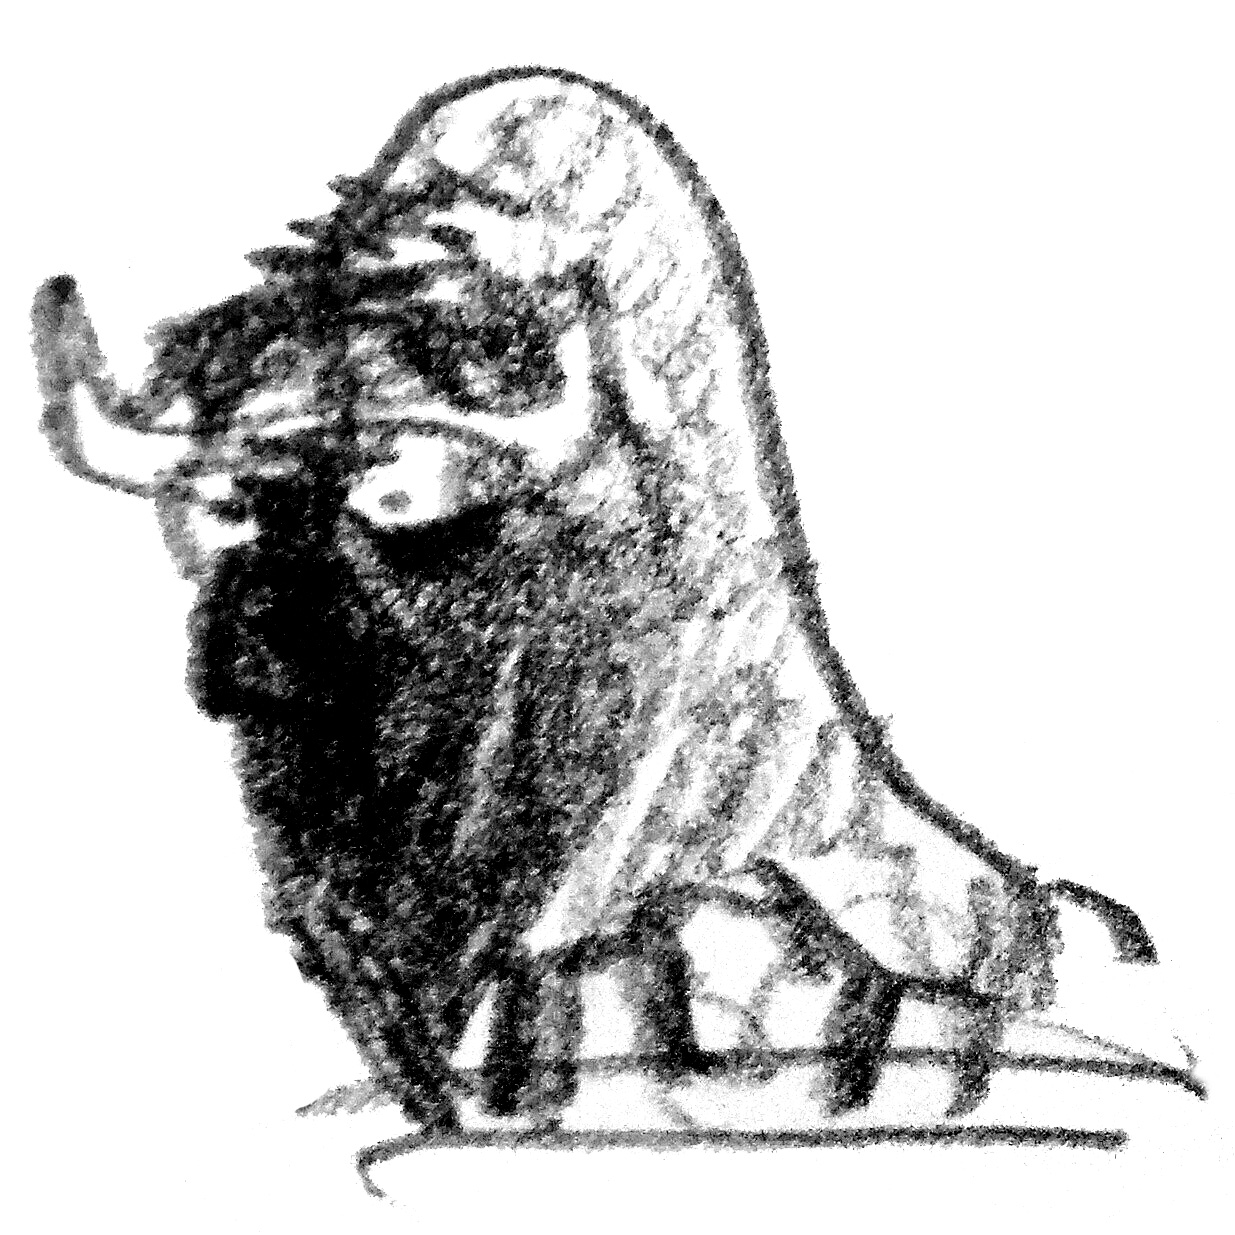
\includegraphics[height=1em]{bison/bison-qed.jpg}}}

\newcommand{\cpother}[1]{{\color{BlueGreen} #1}}
\newcommand{\cpmine}[1]{{\color{GreenYellow} #1}}

% --- my abbreviation ---------------------------------------------------------
\newcommand{\imgsrc}[1]{Image courtesy of #1}
\newcommand{\cfr}[1]{\Cf/ #1}

% --- math models -------------------------------------------------------------
\newcommand{\echoModelFreq}{\ensuremath{
    H_{ij}(f_k) = \sum_{\idxEch=0}^{\numEchs}
        \frac{\absCoeff_{ij}^r}{4 \pi \speedOfSound \tau_{ij}^r}
        \cste^{- \csti 2 \pi k \Fs \tau_{ij}^r / F}}}

\newcommand{\sumEcho}{\ensuremath{\sum_{\idxEch=0}^{\numEchs}}}
\newcommand{\echoModelTimeSimple}[1]{\ensuremath{\sumEcho \alpha_{#1}^{(r)} \delta(t - \tau_{#1}^{(r)})}}
\newcommand{\alltaus}[1]{\ensuremath{\{\tau_{#1}^{(r)}\}_{#1,r}}}
\newcommand{\allalphas}[1]{\ensuremath{\{\alpha_{#1}^{(r)}\}_{#1,r}}}

\newcommand{\icon}[1]{\raisebox{-.1\height}{\includegraphics[height=3ex]{#1}}}
\newcommand{\chaosIcon}{\icon{figures/blaster/chaos.png}}
% --- correct bad hyphenation
\hyphenation{op-tical net-works semi-conduc-tor}

% --- Algos and Methods names:
\newcommand{\mirage}{\textsc{Mirage}}
\newcommand{\separake}{\textsc{Separake}}
\newcommand{\brioche}{\textsc{Brioche}}
\newcommand{\blaster}{\textsc{Blaster}}
\newcommand{\blasterr}{\textsc{Blaster2}}
\newcommand{\lantern}{\textsc{Lantern}}
\newcommand{\dechorate}{d'\textsc{Echorate}}

%----------------
\usepackage{pgffor}
% for math stuff
\foreach \x in {a,...,z}{
  % mathbf
  \expandafter\xdef\csname bf\x \endcsname{\noexpand\ensuremath{\noexpand\mathbf{\x}}}
  % Bold symbol
  \expandafter\xdef\csname bs\x \endcsname{\noexpand\ensuremath{\noexpand\boldsymbol{\x}}}
  % Typewriter
  \expandafter\xdef\csname tt\x \endcsname{\noexpand\ensuremath{\noexpand\mathtt{\x}}}
}

\foreach \x in {A,...,Z}{
%   % Bold symbol -- bold
  \expandafter\xdef\csname bs\x \endcsname{\noexpand\ensuremath{\noexpand\boldsymbol{\x}}}
%   % mathbf -- bold
  \expandafter\xdef\csname bf\x \endcsname{\noexpand\ensuremath{\noexpand\mathbf{\x}}}
%   % mathbb -- blackboard-bold for uppercase letters and lowercase ( for sets )
  \expandafter\xdef\csname bb\x \endcsname{\noexpand\ensuremath{\noexpand\mathbb{\x}}}
%   % mathds -- ???
  \expandafter\xdef\csname ds\x \endcsname{\noexpand\ensuremath{\noexpand\mathds{\x}}}
%   % mathfrak -- gothic
  \expandafter\xdef\csname fk\x \endcsname{\noexpand\ensuremath{\noexpand\mathfrak{\x}}}
%   % mathfrak -- curly
  \expandafter\xdef\csname scr\x \endcsname{\noexpand\ensuremath{\noexpand\mathscr{\x}}}
%   % mathcal -- calligraphy
  \expandafter\xdef\csname cal\x \endcsname{\noexpand\ensuremath{\noexpand\mathcal{\x}}}
}

% --- Math Notation
% math
\newcommand{\Ii}{\ensuremath{\imath}}
% \newcommand{\cstj}{\ensuremath{\jmath}}
\newcommand{\R}{\ensuremath{\bbR}}
\newcommand{\N}{\ensuremath{\bbN}}
\newcommand{\Z}{\ensuremath{\bbZ}}
% indexing
\newcommand{\idxSrc}{\ensuremath{j}}
\newcommand{\idxMic}{\ensuremath{i}}
\newcommand{\idxEch}{\ensuremath{r}}
\newcommand{\numSrcs}{\ensuremath{J}}
\newcommand{\numMics}{\ensuremath{I}}
\newcommand{\numEchs}{\ensuremath{R}}
% geometry
\newcommand{\positionMicrophone}{\ensuremath{\underline{\bfx}}}
\newcommand{\positionSource}{\ensuremath{\underline{\bfs}}}
\newcommand{\positionSurface}{\ensuremath{\underline{\bfp}}}
\newcommand{\pos}{\ensuremath{\bfr}}
\newcommand{\coordinatePermutation}{\ensuremath{\bfR}}
\newcommand{\distMicSrc}{\ensuremath{r}}
\newcommand{\distMicMic}{\ensuremath{d}}
% signal model
\newcommand{\src}{\ensuremath{s}}
\newcommand{\mic}{\ensuremath{x}}
\newcommand{\mics}{\ensuremath{\bsx}}
\newcommand{\img}{\ensuremath{c}}
\newcommand{\imgs}{\ensuremath{\bsc}}
\newcommand{\spat}{\ensuremath{\boldsymbol{\Xi}}}
\newcommand{\master}{\ensuremath{\boldsymbol{\Upsilon}}}
\newcommand{\contRecordedSignal}{\ensuremath{x}}
\newcommand{\contMicrophoneSignal}{\contRecordedSignal}
\newcommand{\contSource}{\ensuremath{s}}
\newcommand{\contFilter}{\ensuremath{h}}
\newcommand{\contFilterHat}{\widehat{\contFilter}}
\newcommand{\contRIR}{\contFilter}
\newcommand{\contNoise}{\ensuremath{n}}
\newcommand{\disRecordedSignal}{\bfx}
\newcommand{\disFilter}{\bfh}
\newcommand{\disFilterHat}{\widehat{\disFilter}}
\newcommand{\RecordedSignalDFT}{\bfX}

% (room) acoustics
\newcommand{\speedOfSound}{\ensuremath{c}}
\newcommand{\cair}{\ensuremath{\speedOfSound_\text{air}}}
\newcommand{\temperature}{\ensuremath{T}}
\newcommand{\rhumidity}{\ensuremath{H}}
\newcommand{\forceVec}{\ensuremath{\bsF}}
\newcommand{\velocity}{\ensuremath{\bsv}}
\newcommand{\pressure}{\ensuremath{p}}
\newcommand{\Pressure}{\ensuremath{P}}
\newcommand{\flux}{\ensuremath{\bsq}}
\newcommand{\density}{\ensuremath{\rho}}
\newcommand{\densityEq}{\density_0}
\newcommand{\mass}{\ensuremath{m}}
\newcommand{\volumeUnit}{\ensuremath{\nu}}
\newcommand{\surface}{\ensuremath{S}}
\newcommand{\volume}{\ensuremath{\calV}}
\newcommand{\impedence}{\ensuremath{Z}}
\newcommand{\impedenceAir}{\ensuremath{\impedence_\text{air}}}
\newcommand{\absCoeff}{\ensuremath{\alpha}}
\newcommand{\reflCoeff}{\ensuremath{\beta}}
\newcommand{\boundariesConditions}{\ensuremath{\calB}}
\newcommand{\wavelength}{\ensuremath{\lambda}}
\newcommand{\ntuple}{\ensuremath{\bsm}}

\newcommand{\depSpaceTime}{\ensuremath{\kparen{\positionMicrophone, t}}}
\newcommand{\pressureSpaceTime}{\ensuremath{\pressure\depSpaceTime}}

% signal processing
\newcommand{\error}{\ensuremath{{\varepsilon}}}
\newcommand{\filterLength}{\ensuremath{{L}}}
\newcommand{\Ts}{\ensuremath{T_s}}
\newcommand{\Fs}{\ensuremath{F_s}}
\newcommand{\zeroVect}{\ensuremath{\mathbf{0}}}
\newcommand{\rir}{\ensuremath{h}}
\newcommand{\rirFreq}{\ensuremath{H}}
\newcommand{\rirs}{\ensuremath{\bsh}}
\newcommand{\rtf}{\ensuremath{\tilde{\rir}}}
\newcommand{\rtfs}{\ensuremath{\tilde{\rirs}}}
\newcommand{\ild}{\ensuremath{\mathtt{ILD}}}
\newcommand{\ipd}{\ensuremath{\mathtt{IPD}}}

% math vars and constant
\newcommand{\spike}[1]{\delta_{#1}}
\newcommand{\opObs}{\calA}
\newcommand{\thr}{\tau_\text{max}}
\newcommand{\algoBraire}{BLASTER}
\newcommand{\algoBsn}{BSN}
\newcommand{\algoCrocco}{IL1C}

% variable
\newcommand{\RT}{\ensuremath{\mathtt{RT}_{60}}}
\newcommand{\DRR}{\ensuremath{\mathtt{DRR}}}
\newcommand{\DER}{\ensuremath{\mathtt{DER}}}
\newcommand{\SNR}{\ensuremath{\mathtt{SNR}}}
\newcommand{\dsetValid}{$\mathbf{\mathcal{D}}^{\:\text{(valid)}}$}
\newcommand{\dsetSNR}{$\mathbf{\mathcal{D}}^{\:\SNR}$}
\newcommand{\dsetRT}{$\mathbf{\mathcal{D}}^{\:\RT}$}

% --- Other (constant)
\newcommand{\const}{\ensuremath{\text{\textit{const.}}}}

\newcommand{\idealLowPassFilter}{\phi}
\newcommand{\disRadonMeasure}{\calM(\Theta)}
\newcommand{\posDisRadonMeasure}{\calM_+(\Theta)}

% \newcommand{\m1}{\mathbf{m}_1}
% \newcommand{\m2}{\mathbf{m}_2}
% \newcommand{\s}{{\mathbf s}}
% \newcommand{\params}{\mathbf{\theta}}

% --- Quantities names

% --- Mathematical Delimiters

% % syntactically named delimiters
% \newdelimcommand{ceil}{\lceil}{\rceil}
% \newdelimcommand{floor}{\lfloor}{\rfloor}
% \newdelimcommand{angles}{\langle}{\rangle}
% \newdelimcommand{parens}{\lparen}{\rparen}
% \newdelimcommand{bracket}{[}{]}
% \newdelimcommand{braces}{\lbrace}{\rbrace}
% \newdelimcommand{verts}{\lvert}{\rvert}
% \newdelimcommand{Verts}{\lVert}{\rVert}

% % semantically named delimiters
\newcommand{\set}[1]{\kbrace{#1}}
% \newcommand{\abs}{\verts}
% \newcommand{\size}{\verts}
\newcommand{\abs}[1]{\kvbar{#1}}
\newcommand{\norm}[1]{\kvvbar{#1}}
\newcommand{\normTV}[1]{\ensuremath{\norm{#1}_{\mathtt{TV}}}}
% \newcommand{\tuple}{\angles}
% \newcommand{\iprod}{\angles}

% % Automagic `such that' for set comprehension. Inside an automagic
% % delimiter command, the vertical bar will resize appropriately
% % Example:
% %   \set{ x \in W \given x > 0 }
\newcommand{\given}{\;\mdelim\vert\;}


% --- Math operators
\DeclareMathOperator*{\fourierTrans}{\scrF}
\DeclareMathOperator*{\discreteFT}{\bfF}
\DeclareMathOperator*{\divergence}{\nabla\cdot}
\DeclareMathOperator*{\dirac}{\delta}
\newcommand{\average}{\operatornamewithlimits{average}}

% --- Mathematical operators and function
\newcommand{\conv}{\ast}
\newcommand{\diracOf}[1]{\dirac\kparen{#1}}
\DeclareMathOperator*{\phase}{\angle}
\newcommand{\phaseOf}[1]{\phase{#1}}
\newcommand{\magnitudeOf}[1]{\abs{#1}}
\newcommand{\powerOf}[1]{\abs{#1}^2}


% other definition
\newcommand{\myeq}{\mathrel{\overset{\makebox[0pt]{\mbox{\normalfont\tiny\sffamily def}}}{=}}}
\newcommand{\mathspace}{\hspace{1em}}

%%% MACROS
\newcommand{\gc}[1]{{\textcolor{green}{#1}}}
% \newcommand{\gc}[1]{{\textcolor{black}{#1}}}

\newcommand{\gccor}[2]{{\textcolor{red}{[#1 $\rightarrow$ #2]}}}
% \newcommand{\gccor}[2]{{\textcolor{black}{#2}}}

\newcommand{\gccmt}[1]{{\textcolor{blue}{[SE: #1]}}}
%\newcommand{\gccmt}[1]{}

\newcommand{\gcrm}[1]{{\textcolor{magenta}{[#1]}}}
% \newcommand{\gcrm}[1]{{\textcolor{black}{}}}

% --- Table of Contents -------------------------------------------------------
%%% TOC STYLE : check in the dissertation class
% check dissertation class
% %% MINITOC per CHAPTER
\usepackage{minitoc} % must be inserted after any modification of TOC

% --- Graphics ----------------------------------------------------------------
\usepackage{pgfplots}
\pgfplotsset{compat=1.8}
\usepgfplotslibrary{fillbetween} %for fill under curve
\usepackage{tikz}
\usetikzlibrary{calc,patterns,arrows,shapes.arrows,intersections,fadings,shadows.blur}
\usepackage[abs]{overpic}
% \usepackage[percent]{overpic} % provide \put on figures
\graphicspath{{./figures/}{./icons/}{./logos/}}
\DeclareGraphicsExtensions{.pdf,.png,.jpg}
% add pdf pages
\usepackage{pdfpages} % \includepdf[pages=-]{myfile.pdf}
\usepackage{rotating} % provide sidewaystable env
% 2 sub figures
% \usepackage{subcaption}
% \pgfplotsset{%
%     table/search path={./figures/plots/},
% }

% --- Algorithm ---------------------------------------------------------------
\newcommand\mycommfont[1]{\footnotesize\ttfamily\textbf{\textcolor{mygray}{#1}}}
\SetCommentSty{mycommfont}

% --- Bibliopgraphy -----------------------------------------------------------
\bibliography{contents/back_matter/references.bib, contents/back_matter/references_separake.bib, contents/back_matter/references_dechorate.bib}


% --- Include only ------------------------------------------------------------
% \includeonly{   % Of course this list allows many more file
% %  intro,       % should also work with files in different paths
%     chapter1_acoustics,
%     chapter2_processing,
%     chapter3_evaluation,
% %  chapter3
% }

%%%%%%%%%%%%%%%%%%%%%%%%%%%%%%%%%%%%%%%%%%%%%%%%%%%%%%%%%%%%%%%%%%%%%%%%%%%%%%%
%%%%%%%%%%%%%%%%%%%%%%%%%%%%%%%%%%DOCUMENT%%%%%%%%%%%%%%%%%%%%%%%%%%%%%%%%%%%%%
%%%%%%%%%%%%%%%%%%%%%%%%%%%%%%%%%%%%%%%%%%%%%%%%%%%%%%%%%%%%%%%%%%%%%%%%%%%%%%%

\title{Hunting Acoustic Echoes for Auditory Scene Analysis}
\author{Diego DI CARLO}
\date{\today}

\begin{document}
\frontmatter{}

% % front matter / titelei
% recto: halftitlepage / schmutztitelseite, vortitel
\thispagestyle{empty}
{
    \begin{fullwidth}
        \centering
        \hphantom{.}
        \vfill
        {\Huge
            Hunting Echoes\\
            for\\
            Auditory Scene Analysis
        }
        \vfill
        \vfill
    \end{fullwidth}
}

\clearpage{}

% verso: frontispiece / frontiszipzseite, vakatseite
% dedication
\cleardoublepage{}

% recto: titlepage / titelblatt, innentitel
\thispagestyle{empty}
{
    \calccentering{\unitlength}
    \begin{adjustwidth*}{\unitlength}{-\unitlength}
        \raggedleft{}
        {\Huge\color{Burgundy}%
        Hunting Echoes\\
        for Auditory Scene Analysis}\\[\baselineskip]
        {\LARGE%
        Dissertation Thesis}\\[0.2\textheight]
        {\huge%
        Diego \textsc{Di Carlo}}\\[\baselineskip]
        {\LARGE%
        \today}
        \vfill
        \vfill
        {\large%
        Submitted in partial fulfillment of the requirements\\
        for the degree of Doktor der Naturwissenschaften\\[\baselineskip]% (Dr.\ rer.\ nat.)\\[\baselineskip]

        to the\\[\baselineskip]

        Faculty of Mathematics\\
        at Ruhr-Universität Bochum\\[2\baselineskip]
        %Vorgelegt zur Erlangung des\\
        %Doktorgrades der Naturwissenschaften\\
        %an der Fakultät der Mathematik\\
        %der Ruhr-Universität Bochum\\[2\baselineskip]

        \begin{minipage}{0.5\textwidth}
        \begin{tabular}{lr}
            1st\hspace{4pt} Reviewer & Prof.\ Dr. Gregor Leander\\
            2nd Reviewer & Prof.\ Dr.\; Alexander May
        \end{tabular}
        \end{minipage}
        \hspace*{36pt}
        %}\hspace*{-8pt}

        %\vspace{2\baselineskip}
        %Datum der Disputation: 13.\ Dezember 2019
        \vfill
        }
        \vspace*{\baselineskip}
    \end{adjustwidth*}
}

\clearpage{}

% verso: colophon / impressum
\thispagestyle{empty}
\hphantom{.}
\vfill

\section*{Imprint}

\textit{Hunting Echoes for Audtory Scene Analysis}\\
Copyright \textcopyright{} 2020 by \theauthor{}.\\
All rights reserved. Printed in France.\\
Published by the Ruhr-Universität Bochum, Bochum, Germany.

\section*{Colophon}

This thesis was typeset using \LaTeX{} and the \texttt{memoir} documentclass.
It is based on Aaron Turon's thesis \emph{Understanding and expressing scalable concurrency}\footnote{\url{https://people.mpi-sws.org/~turon/turon-thesis.pdf}}, itself a mixture of \texttt{classicthesis}\footnote{\url{https://bitbucket.org/amiede/classicthesis/}} by Andr\'e Miede and \texttt{tufte-latex}\footnote{\url{https://github.com/Tufte-LaTeX/tufte-latex}}, based on Edward Tufte's \emph{Beautiful Evidence}.\\[0.5\baselineskip]
%
The bibliography was processed by Biblatex.
All graphics and plots are made with PGF/Ti\emph{k}Z.\\[0.5\baselineskip]
%
The body text is set 10/14pt (long primer) on a 26pc measure.
The margin text is set 8/9pt (brevier) on a 12pc measure.
Matthew Carter's \textrm{Charter} acts as both the text and display typeface.
Monospaced text uses Jim Lyles's \texttt{Bitstream Vera Mono} (\enquote{Bera Mono}).

\clearpage{}

% recto: dedication or epigraph
\thispagestyle{empty}
\vphantom{.}
\vfill
{%
    \flushright{}
    \emph{Pleasure to me is wonder—the unexplored, the unexpected, \\
    the thing that is hidden and the changeless thing\\
    that lurks behind superficial mutability.}\\
    \hfill--- Howard Phillips \textsc{Lovercraft}
}
\vfill
\vfill

% verso: blank
\clearpage{}

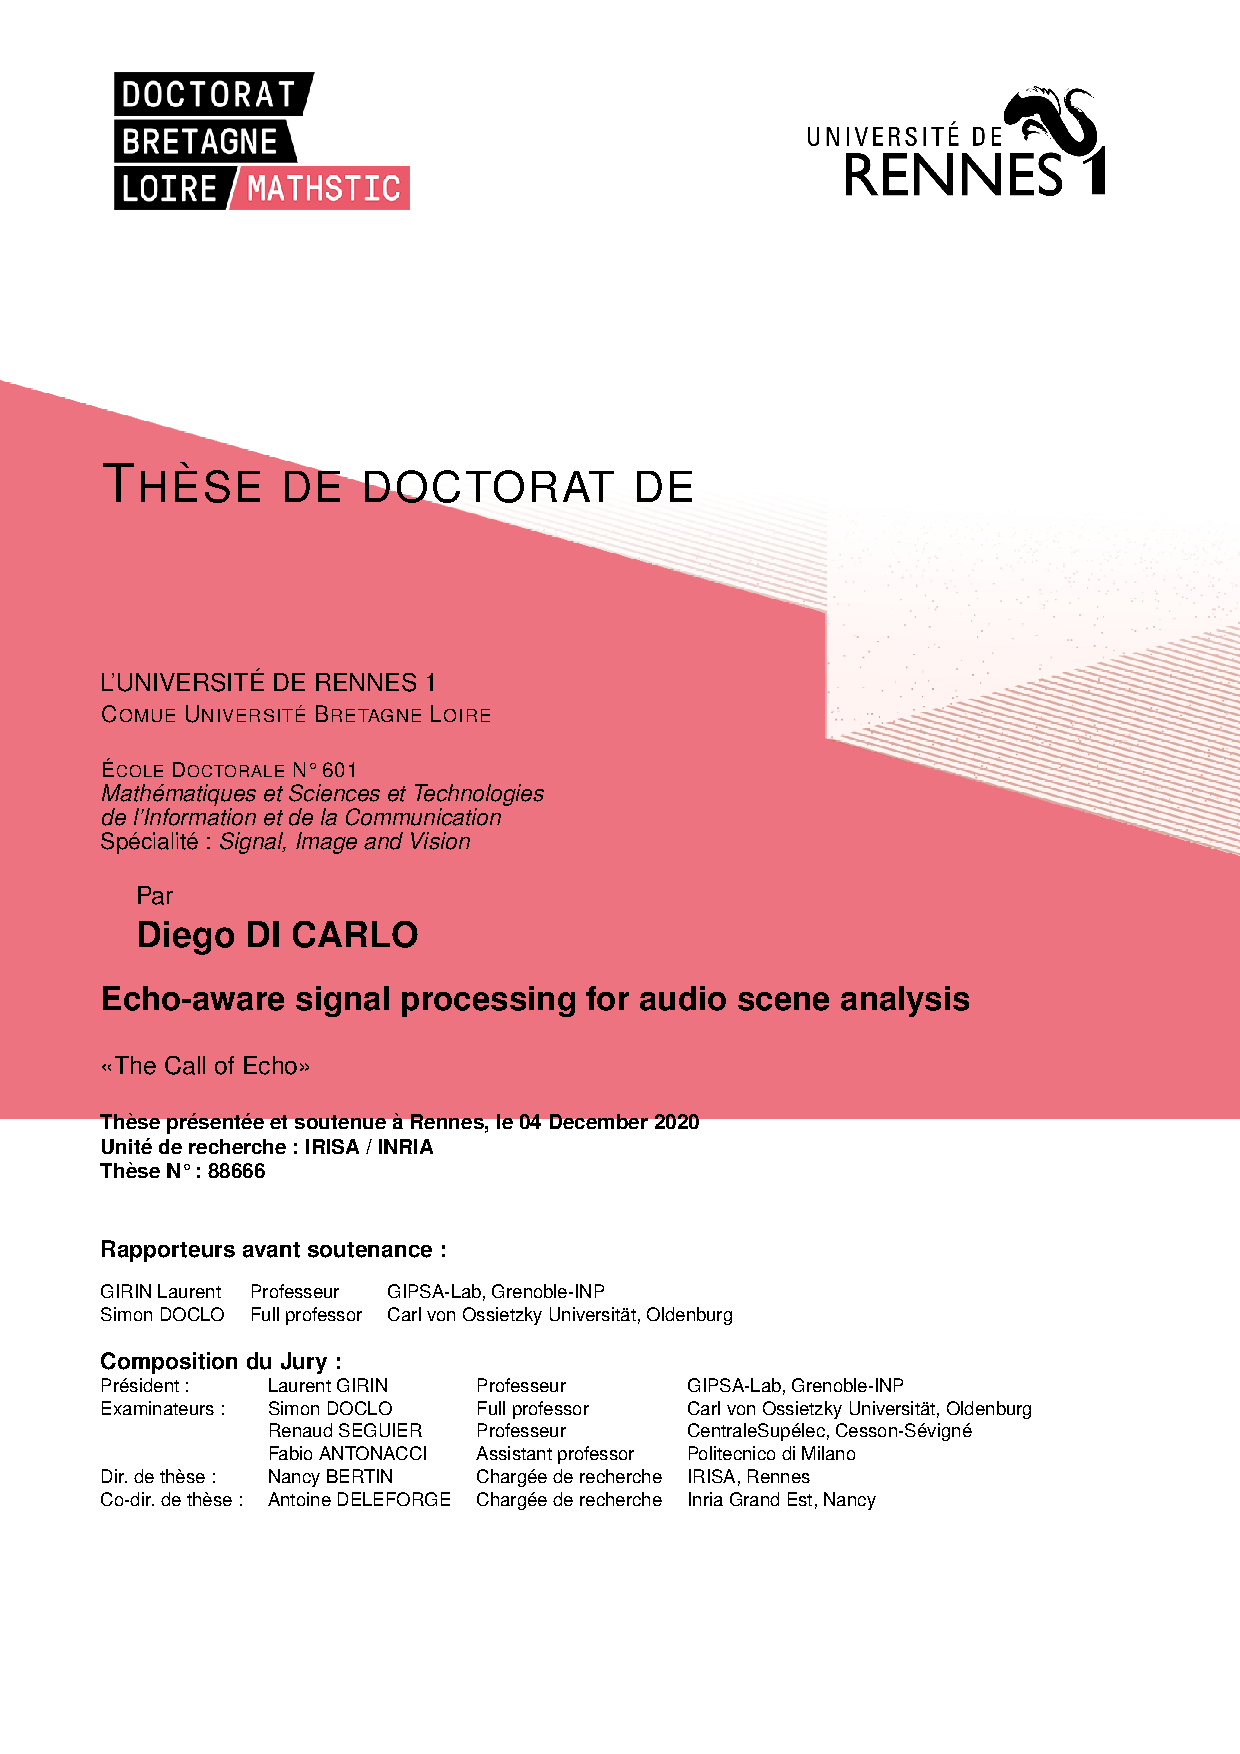
\includepdf[pages=-]{contents/front_matter/mathstic_title_page.pdf}

\chapter*{Abstract}\addcontentsline{toc}{chapter}{Abstract}

Audio\marginpar{
    \footnotesize
    \textbf{Keywords:}
    \\Acoustic echoes, acoustic echo retrieval, room impulse response estimation;
    audio scene analysis, room acoustics;
    audio source separation, room geometry estimation, spatial filtering, sound source localization;
    deep learning, continuous dictionary.
} scene analysis aims at retrieving useful information from microphone recordings.
Examples of these problems are sound source separation and sound source localization, where we are interested in estimating the content and location of multiple sources of sound in an environnement.
As humans, we perform these tasks without effort. However, for computers and robots, they are still open challenges.
One of the main limitations is that most available technologies solve audio scene analysis problems either ignoring how sound propagates in the environment or estimating it fully.

\mynewline
The central theme of this theses is acoustic echoes: the sound propagation elements bridging semantic and spatial information on sound sources.
Indeed, as repetitions of a source signal, their semantic contributions can be aggregated to enhance this signal.
Moreover, since they originate from an interaction with the environment, their paths can be backtracked and used to estimate the audio scene's geometry.
Based on these observations, recent echo-aware audio signal processing methods have been proposed.
However, two main questions arise: how to estimate acoustic echoes, and how to use their knowledge?

\mynewline
This thesis work aims at improving the current state-of-the-art for indoor audio signal processing along these two axes.
It also provides new methodologies and data to process acoustic echoes and surpass current approaches' limits.
To this end, in the first part, we present two approaches:
a novel approach based on the  continuous dictionary framework which does not rely on parameter tuning or peak picking techniques;
a deep learning model estimating the time differences of arrival of the first prominent echoes using physically-motivated regularizers.
Furthermore, we present a novel, fully annotated dataset specifically designed for acoustic echo retrieval and echo-aware applications, paving the way for future echo-aware research.

\mynewline
The second part of this thesis focuses on extending existing methods in audio scene analysis to their echo-aware forms.
The Multichannel NMF framework for audio source separation, the SRP-PHAT localization method, and the MVDR beamformer for speech enhancement are extended to in their echo-aware versions.
These applications show how a simple echo model can lead to a boost in performance.

\newthought{This thesis} highlights the difficulty of exploiting acoustic echoes to improve indoor audio processing.
As a first attempt to lay unified analytical and methodological foundations for these problems, it is hoped to serve as a starting point for promising new research in this field.
% Finally, we want to underline the difficulty related to the tasks of estimating and exploiting acoustic echoes to improve indoor audio processing.
% Therefore, this thesis consists only of a first attempting work that lays analytical foundations on how to model such problems, and it can serve as a starting point for new exciting directions.
\blankpage{}
\chapter*{Résumé en français}\addcontentsline{toc}{chapter}{Résumé en français}

% This summary presents in French an overview of the work addressed in this thesis.

% The audio scene analysis topic covers many different tasks that aim to retrieve useful information from microphone recordings.
% Examples of these problems are sound source separation and sound source localization, where we are interested in estimating a speaker's content and position.
% As humans, we perform these tasks without effort: imagine someone calling us from the other side of the room. Your typical reaction would probably turn your attention towards or even go to him/her.
% However, for computers and robots, using audio signal processing techniques, are still open challenges.

% Sounds convey semantic information (what your friends said), temporal and spatial (when he said it, where he said it).
% We can model these contributions using signals describing the sound content and room impulse response, accounting for its propagation in the space. Some audio processing methods focus on the former, ignoring or roughly describing the latter due to the challenging task of estimating it.
% Room Impulse responses embed all the elements of sound propagation, such as echoes, diffuse reflection, and reverberation.

% The central theme of this theses are acoustic echoes. These elements of sound propagation create a bridge between semantic and spatial information of sound sources. As they are repetitions and copies of the source sound, we can weigh more the target sound by integrating their contribution than other noise sources.
% As these reflections are originated by the interaction of the source sound with the environment, thanks to their arrival time, we can retrace back their paths and, thus, reconstruct the geometry of the audio scene's geometry.
% Based on these observations, audio signal processing methods started to account for these sound propagation elements to solve the audio scene analysis problem.
% Two are the main questions that arise:
% how we estimated acoustic echoes, and how we use their knowledge?

% This thesis work aims at improving the current state-of-the-art for indoor audio signal processing along these two axes.
% In particular, it provides new methodologies and data to process acoustic echoes and surpass current approaches' limits.
% Second, it extends previous classical methods for audio scene analysis in their echo-aware form.
% These two claims are elaborated in the two main parts of the thesis, which follow after an introductory one, as summarized below.

% First, we provide some preliminary definitions of the role of audio signal processing and list some fundamental problems which will be considered throughout the thesis, namely, acoustic echo retrieval, audio source separation, sound source localization, room geometry estimation.

% The~\cref{ch:acoustics} will build a first important bridge: from acoustics to audio signal processing. It first defines sound, how it propagates in the environment, and how this origins echoes.

% In~\cref{ch:processing},  we move from physic to digital signal processing where the echoes are modeled as elements of filters, called Room Impulse Responses (RIRs), operating on the source signal.
% Because processing in the native time domain is complicated, we present the Fourier representation, which facilitates both the exposure of the methods and the implementation of the algorithms.
% This chapter closes the first introductory part.

% In this second part of the thesis, we are interested in estimating early acoustic echoes from microphone recordings. Based on the models and the definition described in the first part, this part includes first a general overview of echo retrieval methods followed by the presentation of two works published at international conferences and a dataset that is about to be released.

% First, in chapter~\cref{ch:estimation}, we provide the reader with knowledge of the state-of-the-art about Acoustic Echo Retrieval, namely, on how to estimate acoustic echoes properties. After presenting the problem and the literature is review according to typical taxonomy used in signal processing. In order to provide a complete look at Acoustic Echo Retrieval, some datasets and evaluation metrics recurring in the literature and used in the following chapter are presented.

% In this second part of the thesis, we are interested in estimating early acoustic echoes from microphone recordings.
% Based on the models and the definition described in the first part, this part includes first a general overview of echo retrieval methods followed by the presentation of two works published at international conferences and a dataset that is about to be released.

% First, in chapter~\cref{ch:estimation}, we provide the reader with knowledge of the state-of-the-art about Acoustic Echo Retrieval, namely, on how to estimate acoustic echoes properties. After presenting the problem and the literature is review according to typical taxonomy used in signal processing. In order to provide a complete look at Acoustic Echo Retrieval, some datasets and evaluation metrics recurring in the literature and used in the following chapter are presented.

% The following three chapters presented three works we conducted on Acoustic Echo Estimation.

% \cref{ch:blaster} presents a novel approach for estimating echoes from a stereophonic recording of an unknown sound source such as speech.  In contrast with existing methods, it is built on the recent continuous dictionary framework and does not rely on parameter tuning or peak picking techniques.
% The method's accuracy and robustness are assessed on challenging simulated setups with varying noise and reverberation levels and are compared to two state-of-the-art methods. Experimental evaluation on synthetic data shows that comparable or slightly worse recovery rates are observed for recovering seven echoes or more. Instead, better results are obtained for a fewer number of echoes, and the off-grid nature of the approach yields generally smaller estimation errors.
% Nevertheless, this is promising since the practical advantage of knowing the timing few echoes per channel will be demonstrated in the last part of the thesis.

% In~\cref{ch:lantern}, we deploy deep learning techniques to estimate acoustic echoes properties. To the best of our knowledge, this is one of the first examples in these directions. The proposed method shares some common grounds with deep learning techniques already applied in sound source localization. We will present three different architecture which addresses the acoustic echo estimation problem with increasing order of complexity: estimating the time of arrival of the direct path and the first prominent echos; perform this estimation in a more robust way; and, finally, extend it to an increasing number of echoes.

% Finally, to conclude this second part, in~\cref{ch:dechorate}, we describe a dataset we collected, specifically designed for acoustic echo estimation. This dataset features measured multichannel room impulse response (RIRs), including annotations of early echoes and 3D positions of microphones and real and image sources under different wall configurations in a cuboid room. These data provide a new tool for benchmarking recent methods in \textit{echo-aware} audio signal processing and software utilities to easily access, manipulate, and visualize the data.

% The third and last part of the thesis concern the audio processing applications where the knowledge of early echoes may improve the performance over standard methods.
% For the occasion, we assume that echoes properties are available a priori and build our prior knowledge.
% The structure of this part follows the format of the previous one.

% An introductory chapter gathers the standard definitions and introduces the current state-of-the-art approaches for indoor audio processing under the same umbrella.
% We consider three fundamental problems: audio source separation, sound source localization, spatial filtering, and room geometry estimation.
% These problems are presented in turn with the related literature review, highlighting the current challenges.
% These particular problems will be the protagonist of the following three chapters, presented in their echo-aware form.

% In~\cref{ch:separake}, echoes are used for boosting the performance of classical Audio Source Separation methods and results from a collaboration with other colleagues, published in an international conference.
% In particular, we propose a physical interpretation of the echoes, namely, image microphones, which allow understanding better how the algorithms benefit from their knowledge.
% Our investigation considers two variants of the multichannel nonnegative matrix factorization source separation framework: one that uses only magnitudes of the transfer functions and uses the phases.
% The results show that the proposed approach beats its vanilla variant by using only a few echoes and echoes enable separation where it was considered unaffordable.

% \cref{ch:mirage} addresses the problem of audio source localization in the context of strong acoustic echoes. Using the model of image microphones presented in the previous chapter, we show that these interfering contributions can be used to change the classic way source localization performed.
% In particular, we show that in a simple scenario involving two microphones close to a reflective surface and one source, the proposed approach is able to estimate both azimuthal and elevation angles, impossible task assuming an ideal propagation, as classical approaches do.
% These results were merged into a publication, published in an international conference.
% Furthermore, the investigation is then extended to microphone arrays featuring multiple sensors and to real-world data, provided by a collaboration with the research team of Honda.

% The ~\cref{ch:dechorateapp} presents two echo-aware applications that can benefit from the dataset \dEchorate, presented in~\cref{ch:dechorate}. We exemplify the utilization of these data considering two possible audio scene analysis problems: echo-aware spatial filtering and room geometry estimation.
% In order to validate the data and show their potential, well-known state-of-the-art algorithms are used. Therefore, for each of the applications, the considered methods are contextualized and summarized.
% Numerical results confirm the value of this dataset for the audio signal processing community. The dataset and these methods will be released publicly so that external contributors will be invited to use them for developing more robust audio processing methods.

% The last chapter (\cref{ch:conclusing}) recapitulates the main results presented in this manuscript and the perspectives related to this work.
% Among them, we show how few acoustic echoes can be estimated from the only observation of microphone recordings featuring reverberant speech using either model derived from the physics of the sound propagation and deep learning models trained on acoustic simulators.
% Moreover, we demonstrate the strengths of including the knowledge of acoustic echoes in audio processing methods.
% For the aspect related to the evaluation of echo-aware methods in a real-world scenario, we advocate that freely-available benchmarking datasets are currently missing in the literature. Therefore, in the spirit of open research, we build a new dataset which will soon be released. These data are accompanied by accurate annotation and algorithmic tools for echo-aware research covering much application for audio scene analysis.

% Finally, we want to underline the difficulty related to the task of estimating and exploiting acoustic echoes to improve indoor audio processing. This thesis, therefore, consists only in a first attempting work that lays analytical foundations on how to model such problems.
% Like all the first investigations, a lot can be improved, and we hope it can serve as a starting point for new interesting, and challenging researches.
\blankpage{}

\chapter*{Acknowledgements}\addcontentsline{toc}{chapter}{Acknowledgements}

Block ciphers form, without doubt, the backbone of today's encrypted communication and are thus justifiably the workhorses of cryptography.
While efficiency of modern designs improved ever since the development of the DES and AES, the case with the corresponding security arguments differs.
The thesis at hand aims at two main points, both in the direction of improving security analysis of block ciphers.

Part~I studies a new notion for the better understanding of a special type of cryptanalysis and proposes a new block cipher instance.
This instance comes with a tight bound on any differential, to the best of our knowledge the first such block cipher.

Part~II turns to automated methods in design and analysis of block ciphers.
Our main contribution here is an algorithm to propagate subspaces through encryption rounds, together with two applications: an algorithmic security argument against a new type of cryptanalysis and an idea towards the automation of key recovery attacks.

\cleardoublepage{}

%*******************************************************
% Table of Contents
%*******************************************************
\doparttoc[n]
\tableofcontents*\addcontentsline{toc}{chapter}{Contents}
\clearpage{}

% \chapter{Glossary}*\addcontentsline{toc}{chapter}{Glossary}%
\marginpar{
    \footnotesize
    \textbf{Glossary:}
    \begin{itemize}
        \item A list of terms in a particular domain of knowledge with their definitions.
        \item From Latin \textit{glossarium} ``collection of glosses'', diminutive of \textit{glossa} ``obsolete or foreign word''.
    \end{itemize}
}
% === GLOSSARY ===
\begin{acronym}[UMLX]
    \acro{AB}{Almost Bent}
    \acro{ACT}{Autocorrelation Table}
    \acro{AES}{Advanced Encryption Standart}
    \acro{ANF}{Algebraic Normal Form}
    \acro{APN}{Almost Perfect Nonlinear}
    \acro{ASIC}{Application Specific Integrated Circuit}
    \acro{BCT}{Boomerang Connectivity Table}
    \acro{BCT}{Boomerang Connectivity Table}
    \acro{CBC}{Cipher Block Chaining}
    \acro{CCA}{Chosen Ciphertext Attack}
    \acro{CFB}{Cipher Feedback}
    \acro{CPA}{Chosen Plaintext Attack}
    \acro{CTR}{Counter}
    \acro{DDT}{Difference Distribution Table}
    \acro{DES}{Data Encryption Standart}
    \acro{DLCT}{Differential-Linear Connectivity Table}
    \acro{DP}{Differential Probability}
    \acro{ECB}{Electronic Codebook}
    \acro{EDP}{Expected Differential Probability}
    \acro{ELP}{Expected Linear Potential}
    \acro{FPGA}{Field Programmable Gate Array}
    \acro{IoT}{Internet-of-Things}
    \acro{KPA}{Known Plaintext Attack}
    \acro{LAT}{Linear Approximation Table}
    \acro{LFSR}{Linear Feedback Shift Register}
    \acro{LP}{Linear Potential}
    \acro{LUT}{Look Up Table}
    \acro{LWC}{Lightweight Crypto}
    \acro{MDS}{Maximum Distance Separable}
    \acro{MEDP}{Maximum Expected Differential Probability}
    \acro{MELP}{Maximum Expected Linear Potential}
    \acro{MILP}{Mixed Integer Linear Program}
    \acro{OFB}{Output Feedback}
    \acro{OTP}{One Time Pad}
    \acro{PRP}{Pseudo\-random Permutation}
    \acro{SLP}{Straight-Line Program}
    \acro{SPN}{Substitution Permutation Network}
    \acro{WSN}{Whitened Swap-Or-Not}

    % --- ch:intro
    \acro{CASA}{Computational Auditory Scene Analysis}
    % --- ch:acoustics
    \acro{SOTA}{State of the Art}
    \acro{GA}{Geometrical (room) acoustics}
    \acro{FEM}{Finite Element Method}
    \acro{BEM}{Boundary Element Method}
    \acro{FDTD}{Finite-Difference-Time-Domain}
    \acro{DWM}{Digital Waveguide Mesh}
    \acro{ISM}{Image Source Method}
    \acro{TOA}{Time of Arrival}
    \acro{RIR}{Room Impulse Response}
    \acro{ReIR}{Relative Impulse Response}
    \acro{FIR}{Finite Impulse Resposne}
    \acro{ATF}{Acoustic Transfer Function}
    \acro{AIR}{Acoustic Impulse Response}
    \acro{TF}{Time-Frequency}
    % --- ch:processing
    \acro{SE}{Speech Enhancement}
    \acro{SSS}{Sound Source Separation}
    \acro{SSL}{Sound Source Localization}
    \acro{RooGE}{Room Geometry Estimation}
    \acro{AER}{Acoustic Echo Retrieval}
    \acro{FT}{Fourier Transform}
    \acro{DFT}{Discrete Fourier Transform}
    \acro{DTFT}{Discrete-Time Fourier Transform}
    \acro{STFT}{Short Time Fourier Transform}
    \acro{FFT}{Fast Fourier Transform}
    \acro{RTF}{Relative Transfer Function}
    \acro{ILD}{Interchannel Level Difference}
    \acro{IPD}{Interchannel Phase Difference}
    \acro{ITD}{Interchannel Time Difference}
    \acro{TDOA}{Time Difference of Arrival}
    \acro{AWGN}{Additive White Gaussian Noise}
    % --- ch:aer
    \acro{AER}{Acoustic Echo Retrieval}
    \acro{MLS}{Minimum Length Sequence}
    \acro{ESS}{Exponential Sine Sweep}
    \acro{ML}{Maximum Likelihood}
    \acro{MUSIC}{Multiple Signal Classification}
    \acro{ESPRIT}{Estimation of Signal Parameters via Rational Invariance Techniques}
    \acro{SSL}{Sound Source Localization}
    \acro{RooGE}{Room Geometry Estimation}
    \acro{JADE}{Joint Angle and Delay Estimation}
    \acro{DOA}{Direction of Arrival}

\end{acronym}
\cleardoublepage{}
\clearpage{}

% \listofalgorithms\addcontentsline{toc}{chapter}{List of Algorithms}
% \vspace{\baselineskip}
% \clearpage{}
% %*******************************************************
% % List of Figures
% %*******************************************************
% \listoffigures*\addcontentsline{toc}{chapter}{List of Figures}
% \vspace{\baselineskip}
% \clearpage{}

% \listoftables*\addcontentsline{toc}{chapter}{List of Tables}
% \clearpage{}

\chapter*{Notations}\addcontentsline{toc}{chapter}{Notations}\label{ch:notation}

\section*{Linear Algebra}
\begin{table}[H]
    \begin{tabular}{ll}
        $x, X$     & scalars      \\
        $\bsx, \bfx$  & vectors      \\
        $x_i$   & $i$-th entry of $\bfx$ \\
        $\zeroVect_I$ & $I\times1$ vector of zeros\\
        $\ktranspose{\bfx}$   & transpose of the vector $\bfx$ \\
        $\khermitian{\bfx}$   & conjugate-transpose (Hermitian) of the vector $\bfx$ \\
        $\kRe[x]$ & real part scalar (vector) $x$ ($\bfx$) \\
        $\kIm[x]$ & imaginary part scalar (vector) $x$ ($\bfx$) \\
        $\csti$  & imaginary unit \\
        $\bbN$    & set of natural numbers \\
        $\bbR$    & set of real numbers \\
        $\bbR_{+}$  & set of real positive numbers \\
        $\bbC$      & set of complex numbers \\
    \end{tabular}
\end{table}

\section*{Common indexing}
\begin{table}[H]
    \begin{tabular}{ll}
        $i$     & microphone or channel index in $\{0, \ldots, I-1\}$      \\
        $j$     & source index in $\{0, \ldots, J-1\}$      \\
        $r$     & reflection (echo) index in $\{0, \ldots, R-1\}$      \\
        $t$     & continuous time index\\
        $n$     & discrete sample index in $\{0, \ldots, N-1\}$ \\
        $f$     & continuous frequency index in $\set{0, \ldots, T-1}$\\
        $k$     & discrete frequency index in $\{0, \ldots, F-1\}$ \\
        $l$     & discrete time-frame index in $\{0, \ldots, L-1\}$\\
        $\tau$  & continuous tap index
    \end{tabular}
\end{table}

\section*{Geometry}
\begin{table}[H]
    \begin{tabular}{ll}
        $\positionMicrophone_i$ & 3D position of the microphone $i$ recording $x_i(t)$\\
        $\positionSource_j$ & 3D position of the source $j$ emitting $s_j(t)$\\
        $\distMicMic_{ii'}$           & distance between microphone $i$ and $i'$ \\
        $\distMicSrc_{ij}$     & distance between microphone $i$ and source $j$ \\
        $r_{j}$    & distance of source $j$ \wrt/ to a reference frame \\
        $\theta_{j}$    & azimuth of source $j$ \wrt/ to a reference frame\\
        $\varphi_{j}$    & elevation of source $j$ \wrt/ to a reference frame \\
        $\vartheta_{j}$    & angle of arrival of source $j$ \wrt/ to a reference frame \\
    \end{tabular}
\end{table}

\section*{Signals}
\begin{table}[H]
    \begin{tabular}{ll}
        $\tildex(t)$    & continuous time domain signal\\
        $x[n]$          & discrete time domain signal\\
        $x_N[n]$          & discrete and finite time domain signal\\
        $\tildeX(f)$    & continuous frequency domain\\
        $X[k]$          & discrete frequency domain\\
        $X[k,l]$        & discrete time domain\\
                        &                     \\
        $x_i$     & input signal recorded at microphone $i$\\
        $\bsx$    & $I \times 1$ multichannel input signal, i.e. $\bfx = [x_0, \ldots, x_{I-1}]$ \\
        $\bsH$    & matrix of multichannel signal or filters, typically the mixing matrix ($I \times J$)\\
        $s_j$     & (target) point source signal $j$ \\
        $q_j$     & (interfering) point source signal $j$ \\
        $c_{ij}$  & spatial image source $j$ as recorded at microphone $i$\\
        $a_{ij}$  & acoustic impule response from source $j$ to microphone $i$ \\
        $h_{ij}$  & generic filter from source $j$ to microphone $i$ \\
        $n_{i}$   & (white \textbf{or} distortion) noise signal at microphone $i$\\
        $u_{i}$   & generic interfering \textbf{and} distortion noise signal at microphone $i$ \\
        $\varepsilon_{i}$   & generic noise signal due to mis- or under-modeling $i$ \\
    \end{tabular}
\end{table}

\section*{Acoustic}
\begin{table}[H]
    \begin{tabular}{ll}
        $\alpha_{r}$    & attenuation coefficient at reflection $r$\\
        $\beta_{r}$     & reflection coefficient at reflection $r$\\
        $\tau_{r}$      & time instant of the reflection $r$\\
        $\cair$         & speed of sound in air\\
        $\temperature$  & temperature\\
        $\rhumidity$    & relative humidity\\
        $\pressure$     & sound pressure\\
        $\rir_{ij}$     & Room Impulse Response from source $j$ to microphone $i$ \\
    \end{tabular}
\end{table}

\section*{Mathematical Operations}
\begin{table}[H]
    \begin{tabular}{ll}
        $\convCont$          & continuous time convolution\\
        $\convDis$       & discrete linear convolution\\
        $\convCir$       & discrete circular convolution\\
    \end{tabular}
\end{table}

% \section*{Examples}

% Simple time domain echo model:
% \begin{equation*}
%     a_i(t) = \echoModelTimeSimple{}
% \end{equation*}
\newcommand{\synopsisChAcoustics}{
    This chapter will build a first important bridge: from acoustics to audio signal processing.
    It first defines sound and how it propagates in the environment~\cref{ch:acoustics:sec:wave}, teasing out the fundamental concepts of this thesis: the echoes.~\cref{ch:acoustics:sec:reflection} and the \RIRdef/~\cref{ch:acoustics:sec:rir}.
    By assuming some approximations, the \RIR/ will be described in all its parts in relation with methods to compute them.
    Finally, in~\cref{ch:acoustics:sec:perception}, how the human auditory system perceives reverberation will be reported.
}
\newcommand{\synopsisChProcessing}{
    Let us now move from the physics to digital signal processing.
    At first in~\cref{sec:processing:model}, this chapter formalizes fundamental concepts of audio signal processing such as signal, mixtures and noise in the time domain.
    In~\cref{sec:processing:domains}, we will present the signal representation that we will use throughout the entire thesis: the \STFTdef/.
    Finally, after assuming the narrowband approximation, in~\cref{sec:processing:rirmodels} some important models for the \RIRdef/ are described.
}
\newcommand{\synopsisChEstimation}{
This chapter amis to provide the reader with knowledge of the state-of-the-art of \AERdef/.
After presenting the \AER/ problem in~\cref{sec:estimation:problem}, the chapter is divided into three main sections:
\cref{sec:estimation:taxonomy} defines the categories of methods thank to which the literature can be clustered and analyzed in detail later in~\cref{sec:estimation:sota}.
Finally, in~\cref{sec:estimation:datametrics} some datasets and evaluation metrics for \AER/ are presented.
}

\newcommand{\synopsisChBlaster}{
This chapter proposes a novel approach for \textit{off-grid} \AER/ from a stereophonic recording of an unknown sound source such as speech.
In contrast with existing methods, the proposed approach, named \BLASTERdef/.
It is built on the recent framework of \CDdef/ and it does not rely on parameter tuning nor peak picking techniques by working directly in the parameter space of interest.
The accuracy and robustness of the method are assessed on challenging simulated setups with varying noise and reverberation levels and are compared to two state-of-the-art methods.
While comparable or slightly worse recovery rates are observed for the task of recovering 7 echoes or more, better results are obtained for fewer echoes and the off-grid nature of the approach yields generally smaller estimation errors.
}

\newcommand{\synopsisChLantern}{
    This chapter
}

\newcommand{\synopsisChSeparake}{
    In this chapter echoes are used for boosting the performance of classical Audio Source Separation methods.
    At first, we describe existing methods, which typically either ignore the acoustic propagation, or attempt to estimate it fully.
    % Instead, thanks to the geometric interpretation of early echoes, we show how this gives us enough spatial diversity to get a performance boost over the anechoic case.
    Instead, this works investigate whether sound separation can benefit from the knowledge of early acoustic echoes derived from the known locations of a few \textit{image microphones}.
    The improvements are show for two variants of a method based on non-negative matrix factorization: one that uses only magnitudes of the transfer functions, and one that also uses the phases.
    The experimental part shows that the proposed approach beats its vanilla variant by using only a few echoes, and that with magnitude information only, echoes enable separation where it was previously impossible.
}

\newcommand{\synopsisChDechorate}{
    This chapter presents \dEchorate{}: a new database of measured multichannel room impulse response (RIRs) including annotations of early echoes and 3D positions of microphones, real and image sources under different wall configurations in a cuboid room.
    These data provide a tool for benchmarking recent methods in \textit{echo-aware} speech enhancement, room geometry estimation, RIR estimation, acoustic echo retrieval, microphone calibration, echo labeling and reflectors estimation.
    The database is accompanied with software utilities to easily access, manipulate and visualize the data as well as baseline methods for echo-related tasks.
}

\newcommand{\synopsisChDecharateApp}{
    This chapter presents two echo-aware applications that can benefit from the dataset \dEchorate.
    In particular, we exemplify the utilization of these data considering two possible use-cases: echo-aware speech enhancement (\cref{sec:dechorateapp:se}) and room geometry estimation (\cref{sec:dechorateapp:rooge}).
    This investigation is conducted by using state-of-the-art algorithms described and contextualized in the corresponding sections.
    In the final section, (\cref{sec:dechorateapp:conclusion}) the main results are summarized and future perspective will be presented.
}

\cleardoublepage{}

\setcounter{mtc}{9}

% === MAIN BODY ===
\mainmatter{}

% PROLOGE
\begin{fullwidth}
    \part{Prologue}
\end{fullwidth}
\parttoc[n]
\cleardoublepage{}

\chapter{Overture}\label{chap:intro}

\openepigraph{Only echoes answer me.}{Anton Chekhov, Swan Song}
\openepigraph{\textsc{Écho.} Citer ceux du Panthéon et du pont de Neuilly. }{Gustave Flaubert, Dictionnaire des idées reçues}

\section{Preamble}
Animals and humans have a remarkable ability to listen to the acoustic response of their environment.
Also known as \emph{echolocation} or \emph{bio-sonar}, it is used consciously and unconsciously to retrieve
information about the environment and objects using sound waves.
Two (of the most) striking examples are bats and whales which use it as navigation and foraging mechanisms.


\marginpar{%
    \begin{itemize}
        \item[\faYoutube] \href{https://www.youtube.com/watch?v=lLUcOFwZvyY&t=22s}{Testing The World's Longest Echo}
        \item[\faYoutube] \href{https://www.youtube.com/watch?v=px3oVGXr4mo}{What Does Sound Look Like? | SKUNK BEAR}
        \item[\faYoutube] arte
    \end{itemize}

}

Definitions of: In this thesis, an \textit{auditory scene} consists in \textit{sound sources}, \textit{microphones} deployed in a room.


\section{The Problem}\label{sec:intro:problem}
\subsection{Audio Signal Processing}
\begin{itemize}
    \item Motivation
    \item Definitions, Function, Characteristics
    \item Current challenges
\end{itemize}
\newthought{Inverse Problem}
Starting with the effects to discover the causes has concerned physicists for centuries.

While in many ways, mixtures are not different to any other audio signal, two research questions stand out prominently: • Can we obtain the sources sj from the mixture x? • Can we find the number of sources J from x? These two questions are addressed in the scientific fields of sound
source separation and source count estimation


Inverse problems appear when we want to see or examine something that we cannot access directly. What we have is an indirect measurement that contains hidden information.

An inverse problem is always a counterpart of a direct problem, as shown in the schematic diagram below. The direct problem is going from object to data, and the inverse problem is about finding the object back from the data.

The assumed few thousand taps. This model was very popular in the early stages of research [48]–[55]. Recently, interest has revived with sparse penalties which account for prior knowledge about the physical properties of AIRs, namely the facts that power concentrates in the direct path and the first early echoes [56]– [60] and that the time envelope decays exponentially [61], but these penalties have not yet been used in a BSS context.

\subsection{Echo-aware Processing}
In the everyday context, when a sound reflection is perceived distinctly is referred to as \textit{echo}.
While phenomenon can be observed clearly in outdoors environment, such in the mountains or within huge buildings,
in closed rooms it is less noticeable. In fact, echoes are usually masked by a general reverberation of the room.

\begin{itemize}
    \item Motivation
    \item Definitions, Function, Characteristics
    \item Current challenges
\end{itemize}

Auralization is the process of rendering audible, by physical or mathematical modelling, the sound field
of a source in a space, in such a way as to simulate the binaural listening experience at a given position in the modelled space

\section{Audio Inverse Problems}\label{sec:processing:inverse}
\cite{kitic2015cosparse}
\openepigraph{Their generality is of such a wide scope that onemayeven argue that solving inverse problems is what signal processing is all about}{Srdan Kiti\'c, \textit{Cosparse regularization of physics-driven inverse problems}}
\openepigraph{everything is an optimization problem}{\citeonly{watson2001nonlinear}}
\marginpar{
    \footnotesize
    One can see the paralelism with the engineering concepts: analysis and sythesis.
}
In~\cref{sec:intro:problem} we have informally defined \textit{inverse problems}, with an emphasis on inverse problems in signal processing.
An inverse problem is a type of a mathematical problem where we start with the observations and we want to estimate model parameters that produced them.
\\Inverse problems pervades all the field of science and engineering:
source localization~\cite{},
image processing~\cite{},
acoustic imaging and tomography~\cite{},
\marginpar{
    \footnotesize
    A historical example are the calculation of the Earth circunference by Eratosthenes in III century b.c.\\
    and the calculations of Adams and Le Verrier which led to the discovery of Neptune from the perturbed trajectory of Uranus.
}

A inverse problems is defined as the counterpart of a \textit{forward}\sidenote{often referred to as \textit{direct}} problem.
Without falling in and deep mathematical formalism and taxonomies which can be found in \citeonly{bal2012introduction},
we will simply consider the following informal definition:
\begin{center}
    \textit{\emph{Forward problem} starts from known input, while \emph{inverse problem} starts from known output~\cite{santamarina2005discrete}.}
\end{center}
Both these problems focus on an operation relating maps objects of interest, called \textit{parameters} or \textit{variables},
to information collected about these objects, called \textit{measurements}, \textit{data} or \textit{observation}.

For instance, in our context, the direct problem may be the estimation of the \RIR/(s) starting from the known room parameters,
and, the related inverse problem would be the estimation of such room properties from the observation of the \RIR/(s).

Formally, a forward problem is defined through a mathematical model, described by a \textit{operation} $\scrM(\cdot)$
mapping \textit{parameters} $x \in \scrX$ to the \textit{observation} (or measurement) $y \in \scrY$:
\begin{equation}\label{eq:processing:model}
    y = \scrM(x)
    .
\end{equation}
Then, the inverse problem defines a method $\kinv{\scrM}$ that ``reverts'' $\scrM$ in order to recover (estimate) $x$ form the observation of $y$.
% The operator $\scrM$ describes our best effort to construct a \textit{model} for the available data $y$.
% The choice of $\scrX$ describes our best effort to characterize the space where we believe the parameters belong.

As discussed in~\cite{bal2012introduction}, \textit{solving} the inverse problem consists in finding point(s) $x \in \scrX$ from (knowledge of) data $y \in \scrY$
such that~\cref{eq:processing:model} or an approximation of~\cref{eq:processing:model} holds.
Under this light, the operator $\scrM$ ant the choice of $\scrX$ describes our best effort to construct a \textit{model} for the data $y$ and
the space where the parameters $x$ belong, respectively.
\marginpar{
    \footnotesize
    one can already see the paralelism the the definition of the mixing process defined in~\cref{sec:intro:problem}
}

\textsc{For instance, in Case of} \textit{linear} inverse problem, and for $\scrY$ and $\scrX$ being vector spaces of dimensions $M$ and $N$ respectively,
then the forward map can be written as a linear system:
\begin{equation}\label{eq:processing:linear_forward}
    \bfy = \bfM \bfx
\end{equation}
where $\bfM$ being a matrix, namely the operator $\scrM$ becomes a matrix multiplication by $M$.
It follows that the inverse map associated to~\cref{eq:processing:linear_forward} is the application of the inverse matrix $\kinv{M}$.
% While solving a direct problem the an operator needs to be found, in solving the inverse one either the operator is known and needs
% to be $reverts$t

Typically, forward problems are considered somehow the ``easier''.
In fact, even in the observation model $\scrM$ is known perfectly, it is not always possible to find its counterpart.
This because of
\begin{itemize}
    \item presence of \textit{noise} in the measurement which are not always additive and statistically independent \wrt/ $x$.
    \item the problem is \textit{well-posed} and \textit{well-conditioned}, namely $\scrM$ needs be injective and stable.
    In other words, some information is recoverable, other is completely lost, other highly sensible to noise
    \sidenote{
        \textbf{injective} ensure the uniqueness of the solution, while \textbf{stability}
        ensure a continuity on the data.
        These are known as the Hadamard's \textit{solvability conditions}.
    }.
\end{itemize}

As we could images, many interesting and fundamental inverse problem are
\textit{ill-posed} or \textit{ill-conditioned} in general, even in the following ``simple'' ones~\cite{kitic2015cosparse}:
The solution to the deconvolution problem, where the direct inversion of the transfer function results in instabilities
at high frequency; and the solution a linear system $\bfy = \bfM \bfx$ where $\bfM$ is invertible
may lead to erroneous results and numerical instabilities.

Therefore, sometimes ones have to settle for restring the set of solution $\scrC \subset \scrX$,
where $\scrM$ is stable and injective\sidenote{This framework was originally proposed by Tikhonov.}.
Promoting solution $x \in \scrC$ is can be achieved through \textit{model priors}, namely prior knowledge about solution, which can
be classified in the following methodologies:
the usage of \textit{geometric constraints} that deterministically define the solutions; the imposition of \textit{penalization}
which ``promotes'' solution of a certain shape (\eg/ \textit{sparse}
\sidenote{\textbf{sparsity} is a fundamental concept of this thesis, better discussed in~\cref{pt:estimation}
} or \textit{smoothness});
and casting the problem in a \textit{bayesian framework} which versatilely incorporate prior and posterior density function describing the data.

\subsection{General Processing Scheme}
Digital signal processing (DSP) is the process of analyzing and modifying a signal to optimize or improve its efficiency or performance. It involves applying various mathematical and computational algorithms to analog and digital signals to produce a signal that's of higher quality than the original signal.
It is traditional in engineering to represent complex systems as a collection of simpler subsystems, with well-defined tasks, interacting with each other.
In signal processing, these subsystems roughly fall into four categories: \textit{representation}, \textit{enhancement}, \textit{estimation}, and \textit{adaptive processing}.
Many problems can be decomposed into blocks that belong to one of these categories.

\begin{description}
    \item[Representation] Objects can be represent (described) in many different way.
    Through different representations, some object \textit{information} becomes more relevant and suitable for certain tasks
    than other.
    \\Representation can be lossy or lossless, and are generally implemented through (non)linear mapping, such as change of basis or feature.
    The most famous representation is the Fourier basis.
    \\Depending on the task the representation may be invertible.
    The process of changing representation is often called: Analysis and Synthesis

    \item[Enhancement] Measurement are affected by noise and interferences which corrupt and hide relevant information, making inverse problems ill-posed and ill-conditioned.
    Therefore, signal enhancement, that is removing noise, is a necessary step.
    \\Enhancement constitute a huge dome of methods: form simple denoising by averaging of repeated measurement to
    spectral subtraction to source separation with neural network.

    \item[Estimation] Often we wish to estimate some key properties of the target signal which may be used as inputs to a different algorithm.

    \item[Adaptive processing] deals with adaptive algorithms and filters controlled by variable parameters.
    A common means to adjust those parameters according to an optimization algorithm which rely on statistical properties of the signal of interest.
    They often implement a kind of online optimization where an objective function is being minimized.
    When new data is observed, its discrepancy with the current estimate is used to produce a new estimate in a way that reduces the objective.
\end{description}

Let us give two example of practical systems that will be recurrent thought out the entire thesis.

\subsection{Selected Audio Inverse Problems}
Here follow some famous problems in the field of audio signal processing with application to speech, music and environmental audio.
Given the mixing process defined in~\cref{sec:processing:model},

% \begin{description}
%     \item[sound source separation and enhancements] as the problem of retrieving a (set of) source signal from a mixture.
%     \item[sound source localization] estimation of source location from the observation of the sound production.
%     This has sense as long as the impulse response convey space properties.
%     \item[microphones calibration] estimation of the microphone placement.
%     \item[\RIR/ estimation] estimation of the filters.
%     Blind Channel Estimation or System Identification.
%     \item[Acoustic Echoes Estimation] estimation of the filters
%     \item[dereverberation] estimation of the filters
%     \item[room geometry estimation] estimation of the room
%     \item[automatich speech recognition]
% \end{description}

\begin{table}[!h]

    \begin{fullwidthfig}
    \centering
    \small

    \begin{tabular}{p{0.33\linewidth}|p{0.66\linewidth}}
        \toprule
        Inverse Problem & \textit{Can we estimate the...} \\
        \hline
        Audio Source Separation  & the signal of the sources $s_{j}$ from the mixture $\boldsymbol{x}$? \\

        Sound Source Localization & the position $\mathbf{s}_{j} \ =\ [ x_{s_{j}} ,\ y_{s_{j}} ,\ z_{s_{j}}]$  of the source $s_{j}$ from the mixture $\boldsymbol{x}$$ $? \\

        Microphone (Array) Calibration & the position of the microphone (array) position $\mathbf{x}$ from the mixture $\boldsymbol{x}$? \\

        \RIR/ Estimation & the filter between the sources $\boldsymbol{s}_{j}$ and the mixture $\boldsymbol{x}$ from $\boldsymbol{x}$? \\

        Room Geometry Estimation & the shape of the room in which the mixture $\boldsymbol{x}$ recoding source $s_{j}$? \\
        \bottomrule
    \end{tabular}

    \end{fullwidthfig}

    \vspace{-\baselineskip}\vspace{-\baselineskip}
    \sideparmargin{outer}
    \sidepar{\vspace{\baselineskip}
        \caption{Selected audio inverse problems}
    }
    \label{tab:processing:problems}


\end{table}

\openepigraph{Everything is connected}{Douglas Adams, \textit{Dirk Gently's Holistic Detective Agency}}
\newthought{Depending on the scenario}, all these problems exhibits strong inter-connections,
namely the solution of one may be (dependent on) the solution of another.
Therefore, exploiting expertise and knowledge,
interconnect and hierarchical approaches may be built\sidenote{Machine Learing allows now for end2end approaches}:
for instance, many spatial filtering techniques used for \SE/ rely on \SSL/ blocks;
and in order to achieves \RooGE/, \AER/ must be done.


\section{My Thesis}
\subsection{Hunting Acoustic Echoes}
\subsection{Echo-aware Auditory Scene Analysis}


\section{Organization and Contributions}
\newthoughtpar{Room Acoustic meets Signal Processing}
\subparagraph{\cref{chap:acoustics}}\blindtext
\subparagraph{\cref{chap:processing}}\blindtext
\subparagraph{\cref{chap:evaluation}}\blindtext

\newthought{Hunting Acoustic Echoes}
\subparagraph{\cref{chap:estimation}}\blindtext
\subparagraph{\cref{chap:lantern}}\blindtext
\subparagraph{\cref{chap:blaster}}\blindtext
\subparagraph{\cref{chap:blasterr}}\blindtext


\newthought{Echo-aware Auditory Scene Analysis}
\subparagraph{\cref{chap:application}}\blindtext
\subparagraph{\cref{chap:separake}}\blindtext
\subparagraph{\cref{chap:mirage}}\blindtext
\subparagraph{\cref{chap:brioche}}\blindtext


Finally, the dissertation concludes with Chapter X, which summarizes
the contributions and raises several additional research questions


\section{This Thesis: Don't Panic!}
The reader will have already noticed that a large margin is left free on the right side of each page of the manuscript.
We will use it to insert comments, historical notes as well as figures and tables to complete the subject.
This graphic charter is inspired by the work of Tufte (2001) and produced using the latex tufte-latex class.
We emphasize that the presence of the clickable GitHub logo in the margin indicates the online availability of the codes.

\newthought{Quick vademecum} for the readers:
\begin{itemize}
    \item Bibliographic references are denoted as \cite{kuttruff2016room}.
    \item Figures, Tables and other floating objects as well as equations are numbered within the chapter number.
    \item Equations are referred as~\cref{eq:acoustics:green_definition}
    \item The main matter of the Thesis’s manuscript starts at page 1, until page 103.
    \item The back matter covers the list of the candidate’s publications and the bibiographic references cited along the text.
    \item Small notes on the margin might be used to easily navigate through the Example of margin note manuscript. They are meant to summarize paragraphs/blocks of text.
    \item The end of the chapter is shown by the following sign between horizontal rules.
\end{itemize}

% % %% I. Room Acoustic
% \begin{fullwidth}
%     \part{Room Acoustic meets Signal Processing}\label{pt:background}
% \end{fullwidth}
% \parttoc[n]
% \chapter{Element of Room Acoustics}\label{chap:acoustics}
\marginpar{%
    \centering
    \footnotesize
    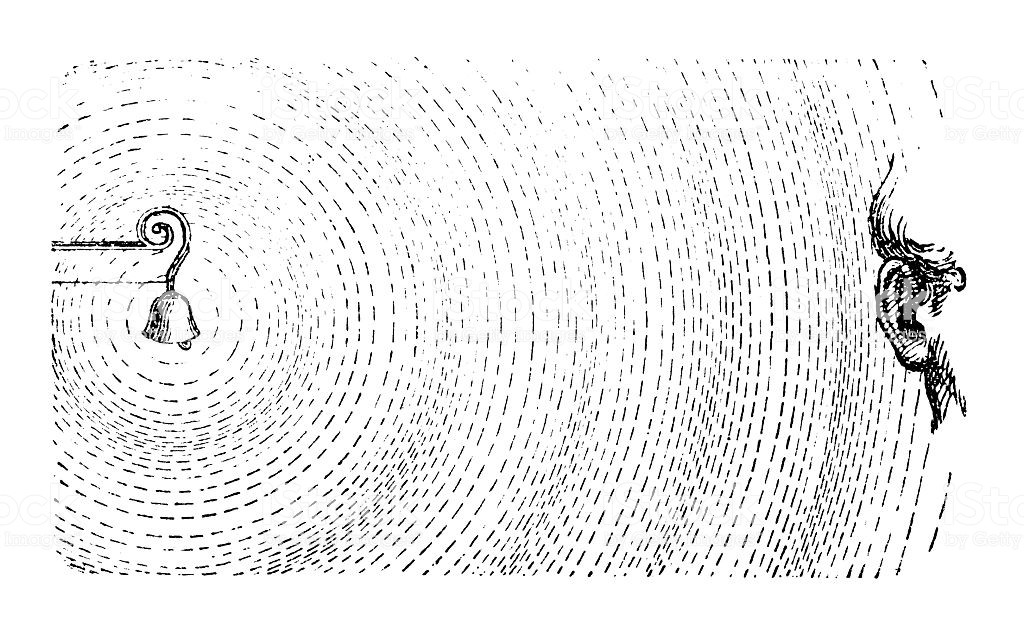
\includegraphics[width=\linewidth]{acoustics/sound_propagation.jpg}
    \label{fig:acoustics:sound}
}
\openepigraph{Sound, a certain movement of air.}{Aristotele, De Anima II.8 420b12}
\vspace{-2.5em}
\newthought{Synopsis}
This chapter will build a first important bridge: from the physics to analog signal processing.
% Acoustics explains how sounds works in environment, while room acoustic explain sound in enclosed spaces, such as living rooms, offices, concert halls and many others.
It first defines sound and how its propagation~\cref{ch:acoustics:sec:wave} connected the concept of impulse response.
Then the interaction with the environment is show~\cref{ch:acoustics:sec:reflection}, teasing out the fundamental concept of this thesis: the echoes.
By assuming some approximation, the \RIRdef/ will be defined.
Finally, a description of the way the human auditory system perceives the sound will be reported.
In particular, the influence of the first early reflection on the sound perception will be elaborated.
One of the most frequently effects produced during sound propagation in a medium is reverberation,
which is caused by physical surfaces that partly absorb and partly reflect sound waves in air. We will first examine in Sec. 4.2 the physical and perceptual background of reverberation. The knowledge gained on these aspects will enable us to study some of the most known reverberation algorithms in Sec. 4.3. Finally we will review in Sec. 4.4 more recent approaches to synthetic reverberation, that are based on feedback delay networks and waveguide meshes.
The rest of the section is reproduce the derivation of this equation, re-arranging the derivation presented in \cite{kuttruff2016room, pierce2019acoustics, marczuk2006modelling, avanzini2019sound}.

\section{Sound Wave Propagation}\label{ch:acoustics:sec:wave}
\marginpar{%
    \small
    Noun: from Middle English sownde, alteration of sowne, borrowed from Anglo-Norman sun, soun, Old French son, from accusative of Latin sonus.
}
According to common dictionaries and encyclopedias,
\begin{center}
    \textit{sound is the sensation perceived by the ear caused by the vibration of air}.
\end{center}
Sound has then two aspects: a physical one, characterized by the vibrating air particles; and a perceptive one, involving the an auditory system.
\marginpar{
    \small
    It is legit to interrogate about where is the sounds.
    % If the sounds we hear have spatial locations, they can be thought to be located either where the material sources are (distal theories), or where the hearers are (proximal theories), or somewhere in between (medial theories). It has also been denied that sounds have any spatial locations, which gives rise to a fourth class of theories, aspatial theories.
    % Proximal theories would claim that sounds are where the hearer is.
    % Medial theories—exemplified by mainstream acoustics—locate sounds in the medium between the resonating object and the hearer.
    % Distal theories consider sounds to be located at the resonating object. Finally, aspatial theories deny spatial relevance to sounds.
}
Focusing on the former phenomenon, when vibrating objects excites air, air molecules starts oscillating,
producing zones with different air densities (compressions-rarefactions)\sidenote{%
Sound needs a medium to travel: it cannot travel through a vacuum.
\\Unfortunately, there is no sound in outer space.
}.
Such vibration of molecules takes place in the direction of the excitement, with the next layer of molecules excited by the first layer.
Pushing layer by layer forward, a \textit{longitudinal wave} is created.
Under a this perspective,
\begin{center}
    \textit{sound is a longitudinal, mechanical wave}.
\end{center}
\marginpar{
    \small
    % In a longitudinal wave the particle displacement is parallel to the direction of wave propagation.
    % In a transverse wave the particle displacement is perpendicular to the direction of wave propagation.
    As opposed to mechanical vibrations in a string or (drum) membrane,
    acoustic vibrations are \textit{longitudinal} rather than \textit{transversal},
    \ie/ the air particles are displaced in the same direction of the wave propagation.
}
A \textit{wave} is a disturbance that propagates though a medium, which could be solid, liquid or gaseous.
\marginpar{%
    \centering
    \footnotesize
    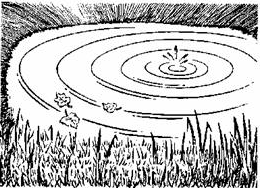
\includegraphics[width=\linewidth]{acoustics/lake.png}
    \captionof{figure}{%
    Imagine a calm pool. The surface is flat and smooth. Drop a rock into it. Kerploop. The surface is now disturbed.
    The disturbance spreads propagates, as well know waves. The medium here is the water surface.
    }
    \label{fig:acoustics:lake}
}
The propagation happens at a certain speed which depends on the physical properties of the medium, such as its density and composition.
The medium assumed through out the entire thesis is air.
Under the fair assumption of air being homogeneous and steady,
the speed of sound can be computed with the following approximated formula:
\begin{equation}
    \cair =  331.4 + 0.6\temperature + 0.0124\rhumidity \hspace{1em} [\sfrac{\si{\metre}}{\si{\second}}]
    ,
\end{equation}
where $\temperature$ is the air temperature $[\si{\celsius}]$ and $\rhumidity$ is the relative air humidity $[\%]$.
The changes in air pressure can be represented by a \textit{waveform}, which is a graphic representation of a sound.

\begin{figure}[h]
    \centering
    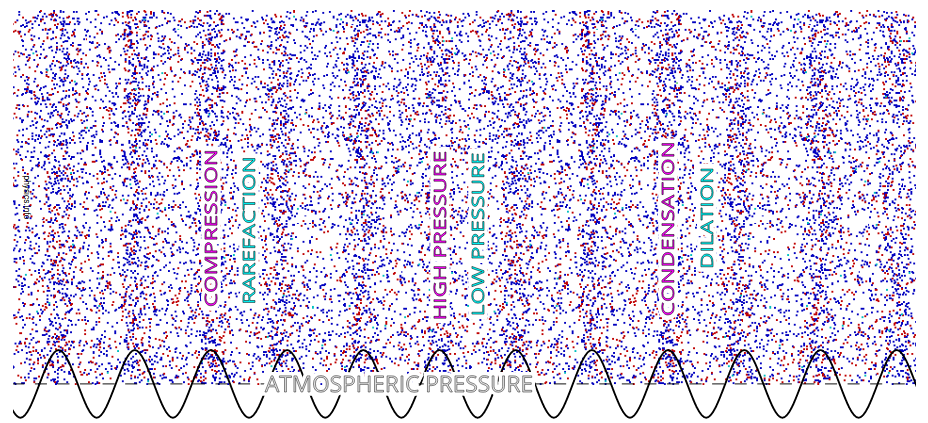
\includegraphics[width=\linewidth]{acoustics/acoustic_wave.png}
    \caption{snapshot of a longitudinal wave in air}
    \label{fig:acoustics:acoustics_wave}
\end{figure}
In general, the sound field is complex which can be decomposed as a superimposition of several waves~\cite{kuttruff2016room}.

We think at this process in the light of the classic \textit{source-medium-receiver} model of communication theory.
\begin{description}
    \item[source] is anything that emits or expends energy (waves)
    \sidenote{%
    example of sources are vibrating solids (\eg/ speakers membrane),
    rapid compression or expansion (\eg/ explosions or implosions)
    or air vortices with characteristics frequencies (\eg/ flute and whistles).
    },
    \item[medium] is the vehicle for carrying waves from one point to another, and
    \item[receiver] absorbs the such waves.
\end{description}

The behavior of acoustic waves is defined by the acoustic-wave equation.
The rest of the section is reproduce the derivation of this equation, re-arranging the derivation presented in \cite{kuttruff2016room, pierce2019acoustics, marczuk2006modelling, avanzini2019sound}.

\subsection{The Acoustic wave equation}\label{subsec:acoustics:waveq}
It is a second-order partial differential equation
\sidenote{
    In 1746, d’Alembert discovered the one-dimensional wave equation for music strings,
    and within ten years Euler discovered the three-dimensional wave equation for fluids.
} which describes the evolution of acoustic pressure $\pressure$
as function of the position $\positionMicrophone$ $[\si{\metre}]$ and time $t$ $[\si{\second}]$
\marginpar{%
    \footnotesize
    The symbol $\knabla^2 = \kpderiv[2]{}{x} + \kpderiv[2]{}{y} + \kpderiv[2]{}{z}$
    stands for the 3-dimensional \textit{Laplacian} operator.
}
\begin{equation}
    \label{eq:acoustics:wave}
    \knabla^2 \pressureSpaceTime - \frac{1}{\speedOfSound^2} \kpderiv[2]{\pressureSpaceTime}{t} = 0
    .
\end{equation}
The constant $\speedOfSound$ is the sound velocity in the medium with dimension $[\frac{\si{\metre}}{\si{\second}}]$.

Assuming the propagation of the wave in a homogeneous medium, one can obtain the equation above by combining three fundamental physical laws:
\begin{itemize}
    \item the \textit{conservation of momentum}\sidenote{In fluidodynamics, it comes with the name of the Euler's equation},
    \item the \textit{conservation of mass}, and
    \item the \textit{polytropic process relation}\sidenote{meaning that the medium is an ideal gas undergoing a reversible adiabatic process}.
\end{itemize}

In general medium are not uniform and features inhomogeneities of two types:
scalar inhomogeneities, \eg/ due to temperature variation,
and vector inhomogeneities, \eg/ due to presence of fans or air conditioning.
Although these affect the underlying assumption of the model, the effect are small in typical application of speech and audio signal processing.
Therefore they are commonly ignored.

\newthoughtpar{The Helmholtz's equation}
The wave equation~\ref{eq:acoustics:wave} is expressed in the space-time domain $\depSpaceTime$.
By applying the temporal Fourier transform, we obtain the \textit{Helmholtz equation}, \ie/
\begin{equation}
    \label{eq:acoustics:helmholtz}
    \knabla^2 P(\positionMicrophone, f) + k^2 P(\positionMicrophone, f) = 0
    ,
\end{equation}
where $k = \frac{2 \pi f}{c}$  is known as \textit{wave number} $[\si{\metre^{-1}}]$, that relates the frequency $f \; [\si{\hertz}]$ and the propagation velocity $c$.

Both the wave equation~\ref{eq:acoustics:wave} and the Helmholtz's equation~\ref{eq:acoustics:helmholtz} are source independent,
namely no source is present in the medium.
Therefore they are called \textit{homogeneous} as the right-hand term is zero.

Normally the sound field is a complex field generated by acoustics sources.
As consequence, the two equation becomes inhomogeneous as some non-zero terms needs to be added to the right-hand sides.

In presence of a sound source producing waves with distribution function $s(t, \positionMicrophone)$, the wave equation can be written
\begin{equation}
    \label{eq:acoustics:source}
    \knabla^2 \pressureSpaceTime - \frac{1}{\speedOfSound^2} \kpderiv[2]{\pressureSpaceTime}{t} = s(t, \positionMicrophone)
    .
\end{equation}
Then, the correspondent Helmholtz's equation writes
\begin{equation}
    \label{eq:acoustics:source_freq}
    \knabla^2 P(\positionMicrophone, f) + k^2 P(\positionMicrophone, f) = - S(\positionMicrophone, f)
    .
\end{equation}

For instance one can assume an infinitesimally small pulsating sphere locate at $\positionSource$ radiating constant acoustic energy at frequency $f$,
\ie/ $S(\positionMicrophone) = \delta(\positionMicrophone - \positionSource)$.
At the receiver position $\positionMicrophone \neq \positionSource$, the Helmholtz's equation writes
\begin{equation}
    \label{eq:acoustics:green_definition}
    \knabla^2 H(f, \positionMicrophone \mid \positionSource)
     + k^2 H(f, \positionMicrophone \mid \positionSource) = - \delta(\positionMicrophone - \positionSource)
    ,
\end{equation}
The function $H(f, \positionMicrophone \mid \positionSource)$ that satisfy \cref{eq:acoustics:green_definition} is the \textit{Green's function}
associated to ~\cref{eq:acoustics:helmholtz}, for which is also a solution.
\\In the next subsection, we will see that the function $H$ can be interpreted as the free-field \textit{Transfer Function}
between the source at $\positionSource$ and the receiver at $\positionMicrophone$.

\subsection{... and its solution as Green's function}
\marginpar{%
    \footnotesize
    By 1950 Green’s functions for Helmholtz’s equation were used to find the
    wave motions due to flow over a mountain  and in acoustics.
    Green’s functions for the wave equation lies with Gustav Robert Kirchhoff (1824–1887),
    who used it during his study of the three-dimensional wave equation.
    He used this solution to derive his famous \textit{Kirchhoff’s theorem}~\citeonly{duffy2015green}.
}
\textsc{The Green's Functions} are mathematical tools for solving linear differential equations with specified initial- and boundary- conditions~\cite{duffy2015green}.
They have been used to solve many fundamental equations, among which \cref{eq:acoustics:helmholtz,eq:acoustics:wave} for both free and bounded propagation.
\begin{center}
    \textit{
    They can be seen as the equivalent concept of the
    \\ \emph{impulse responses
    \sidenote{impulse response in time domain, trasfer fuction in the frequency domain.}}
    used in signal processing.}
\end{center}
Under this light the physic so-far can be rewritten in the vocabulary of the communication theory, namely \textit{input}, \textit{filter} and \textit{output}.

According to Green's method, the equations above can be solved in the frequency domain for arbitrary source as follows:
\marginpar{%
    \footnotesize
    If one ignores the space integal, one can see the close relation with a transfer function.
}
\begin{equation}
    \label{eq:acoustics:helmholz_conv}
    P(f, \positionMicrophone) = \iiint_{\volume_\contSource} H(f, \positionMicrophone \mid \positionSource) S(f, \positionSource) \kdiff\positionSource
    ,
\end{equation}
where $\volume_\contSource$ denotes the source volume,
and  $\kdiff\positionSource =  \kdiff{x_\contSource}\,\kdiff{y_\contSource}\,\kdiff{z_\contSource}$ the  differential  volume element at position $\positionSource$.
\\The requested sound pressure $\pressureSpaceTime$ can now be computed by taking the frequency-directional inverse Fourier transform of \cref{eq:acoustics:helmholz_conv}.

It can be shown \citeonly{kuttruff2016room} that the Green's function for~\cref{eq:acoustics:helmholtz,eq:acoustics:green_definition} writes
\begin{equation}
    \label{eq:acoustics:greenFreeFreq}
    H(f, \positionMicrophone \mid \positionSource) = \frac{1}{4 \pi \norm{\positionMicrophone - \positionSource}} e^{- \frac{\Ii 2 \pi f \norm{\positionMicrophone - \positionSource}}{\speedOfSound}}
\end{equation}
where $\norm{\cdot}$ denotes the Euclidean norm.
\marginpar{
    \footnotesize
    \cref{eq:acoustics:greenFreeFreq,eq:acoustics:greenFreeTime} are respectively the free-field transfer function and the impulse response.
}
By applying the inverse Fourier transform to the result above, we can write the time-domain Green's function as
\begin{equation}
    \label{eq:acoustics:greenFreeTime}
    h(t, \positionMicrophone \mid \positionSource) =
        \frac{1}{4 \pi \norm{\positionMicrophone - \positionSource}}
        \diracOf{t - \frac{\norm{\positionMicrophone - \positionSource}}{\speedOfSound}}
\end{equation}
where $\diracOf{\cdot}$ is the time-directional Dirac delta function.
\\As a consequence, the \textit{free field}, that is in open air without any obstacle, the  sound propagation
incurs a delay $\distMicSrc / c$
and an attention $1 / (4 \pi \distMicSrc)$ as function of the distance
$ \distMicSrc = \norm{\positionMicrophone - \positionSource}$ from source to the microphone.

According to \cref{eq:acoustics:greenFreeTime}, the sound propagate around a point source with a spherical pattern.
When the receiver is far enough from the source, the curvature of the \textit{wavefront} may be ignored.
The waves can be approximated as \textit{plane waves} orthogonal to the propagation direction.
This scenario depicted in \cref{fig:acoustics:planewaves} is known as \textit{far-field}.
\marginpar{%
    \centering
    \footnotesize
    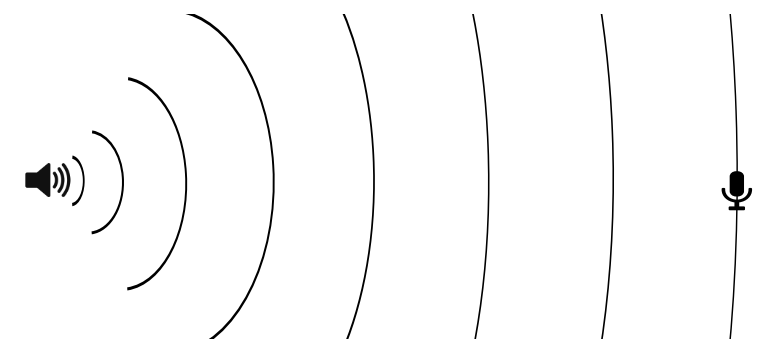
\includegraphics[width=\linewidth]{acoustics/planewaves.png}
    \captionof{figure}{%
    Visualization of the sound propagation. Since the sensor (i.e. a microphone)
    is drawn in the far field, the incoming waves can be approximated as plane waves.
    }
    \label{fig:acoustics:planewaves}
}
As opposed to, when the distance between the source and the receiver is small, the scenario is called \textit{near field}.

%%%%%%%%%%%%%%%%%%%%%%%%%%%%%%%%%%%%%%%%%%%%
\section{Acoustic Reflections}\label{ch:acoustics:sec:reflection}
The equations derived so far assumed unbounded medium, \ie/ free space: a rare scenario in everyday applications.
Real mediums are typically bounded, at least partially.
For instance in a room, the air (propagation medium) is bounded by walls, ceiling, and floor.
When sound travel outdoor, the ground acts as a boundary for one of the propagation direction.
Therefore, the sound wave does not just stop when it reaches the end of the medium or when it encounters an obstacle in its path.
Rather, a sound wave will undergo certain behaviors depending on the obstacle acoustics and geometrical properties, including
\begin{itemize}
    \item \textit{reflection} off the obstacle,
    \item \textit{diffraction} around the obstacle,
    \item and \textit{transmission} into the obstacle, causing
    \begin{itemize}
        \item \textit{refraction} though it, and
        \item \textit{dissipation} of the energy.
    \end{itemize}
\end{itemize}

\marginpar{%
    \centering
    \footnotesize
    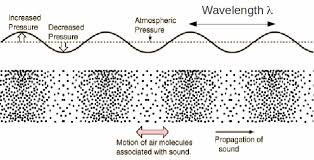
\includegraphics[width=\linewidth]{acoustics/wavelength.jpg}
    \captionof{figure}{%
        wavelength
    }
    \label{fig:acoustics:wavelength}
}
In order, reflections arise typically when a sound wave hit a large surface, like a room wall.
When the sound meets a wall edge or a slit, the wave diffracts, namely it bends around the corners of an obstacle.
The point of diffraction effectively becomes a secondary source which may interact with the first one.
\\The part of energy transmitted to the object may be absorbed and refracted.
Object are characterized by a proper acoustic resistance, called \textit{acoustic impedance}, which
describes its acoustic inertia as well as the energy dissipation.
The remaining contribution may continue to propagate causing resulting in the refraction phenomenon \sidenote{%
    This is more commonly observed when light pass thought different medium, like a prism.
}.

\textsc{When sound reflects} on an solid surface, two type of acoustic reflection can occurs: part of the sound energy
\marginpar{%
    \centering
    \footnotesize
    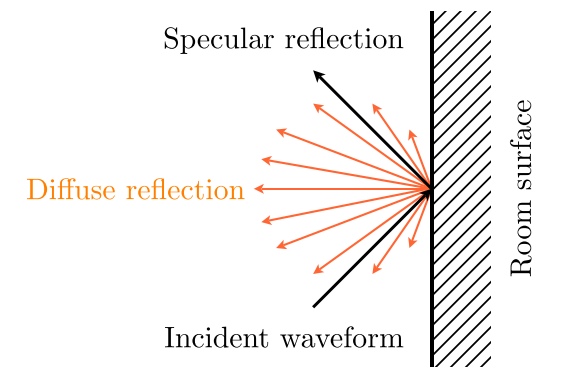
\includegraphics[width=\linewidth]{acoustics/reflection.png}
    \captionof{figure}{%
        Specular vs diffuse reflection
    }
    \label{fig:acoustics:reflection}
}
\begin{itemize}
    \item is reflected \textit{specularly}, \ie/, the angle of incidence equals the angle of reflection; and
    \item is reflected \textit{diffusely} - or \textit{scattered}, \ie/, scatter in every direction).
\end{itemize}

All the phenomena occurs with different proportions depending on the acoustics and geometrical properties of surface and the frequency content of the wave.
In acoustics, it is common to define the \textit{operating points} and different \textit{regimes}\sidenote{for instance near- vs. far-field}
according to the sound frequencies or the correspondent \textit{wavelength} $[\si{\metre}]$,
\begin{equation}
    \wavelength = \frac{2 \pi}{k} = \frac{\speedOfSound}{f} \hspace{1em} [\si{\metre}]
    ,
\end{equation}
where $f$ is the frequency of the sound wave.

\marginpar{
    \footnotesize
    \textit{Sabine had previously used ray-based acoustics in the
    early 1900s to investigate sound propagation paths using Schlieren photography.
    Their impressive visualizations show wavefronts that are augmented
    with rays that are perpendicular to the wavefronts.}
    \\---\citeauthor{savioja2015overview}
}
As depicted in~\cref{fig:acoustics:wavelength}, $\wavelength$ measures the spatial distance between two molecules in the medium having the same value of pressure.
% \marginpar{%
%     \footnotesize
%     a frequency of $\SI{1}{\kHz}$ corresponds to a wavelength of approximately $\SI{34}{\cm}$ ,
%     which is one or two orders of magnitude smaller than typical linear dimensions of rooms,
%     as well as typical distances traveled by sound waves in a room
% }.
\marginpar{
    \centering
    \footnotesize
    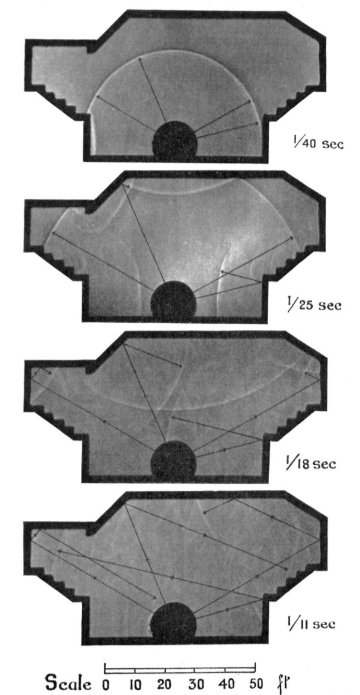
\includegraphics[trim={0 205 0 0},clip,width=\linewidth]{acoustics/sound_pulse1926.png}
    \captionof{figure}{%
        Photographs showing successive stages in the progress of a Sound Pulse in a Model Section of a Debating Chamber.
        \imgsrc{\citeonly{davis1926sound}}
    }
    \label{fig:acoustics:reflection}
}
\\Using this quantity we can identify the following three response of the objects (irregularities) of size $d$ to a plane-wave depicted in~\cref{fig:acoustics:irregularities}
\begin{figure}
    \footnotesize
    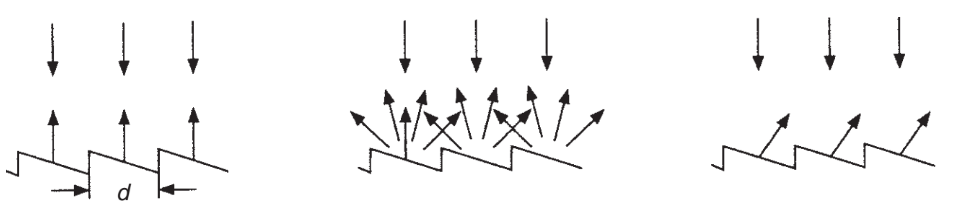
\includegraphics[width=\linewidth]{acoustics/irregularities.png}
    \captionof{figure}{%
        A reflector having irregularities on its surface with width $d$ much smaller than the sound wavelength $\wavelength$.
        Image courtesy of \citeonly{kuttruff2016room}.
    }
    \label{fig:acoustics:irregularities}
\end{figure}
\begin{itemize}
    \item $\wavelength \gg d$, the irregularities are negligible and the sound wave reflection is of specular type;
    \item $\wavelength \approx d$, the irregularities break the sound waves which is reflected towards every direction;
    \item $\wavelength \ll d$, each irregularities is a surface reflecting specularly the sound waves.
\end{itemize}

\textsc{All this presented behavior} can be described with the wave equation imposing opportune boundary conditions.
% However working with this formula might results complicated and difficult.
A simplified yet effective approach - just as in optics - is to model incoming sound waves as \textit{acoustic rays}~\citeonly{davis1926sound, krokstad1968calculating}.
A ray has well-defined direction and velocity of propagation, and conveys a total wave energy which remains constant.
This simplified description undergoes with the name of \GAdef/~\cite{savioja2015overview}, and share many fundamentals with geometrical optics.
This model will be convenient to describe and visualize the reflection behavior hereafter.

\subsection{Large smooth surfaces, absorption and echoes}
% The main focus of this section and the this whole thesis goes on \textit{specular reflections}.
Specular reflection are generated by surfaces which can be modelled as infinite flat, smooth and rigid (\ie/ stationary).
As mentioned above, this assumption is valid as long as the surface has dimension much bigger than the sound wavelength.
Here the acoustic ray is reflected according to the \textit{law of reflection}, stating that
(i) the reflected ray remains in the plane identified by the incident ray and the normal to the surface,
and (ii) the angles of the incident and reflected rays with the normal are equal.
\marginpar{%
    \centering
    \footnotesize
    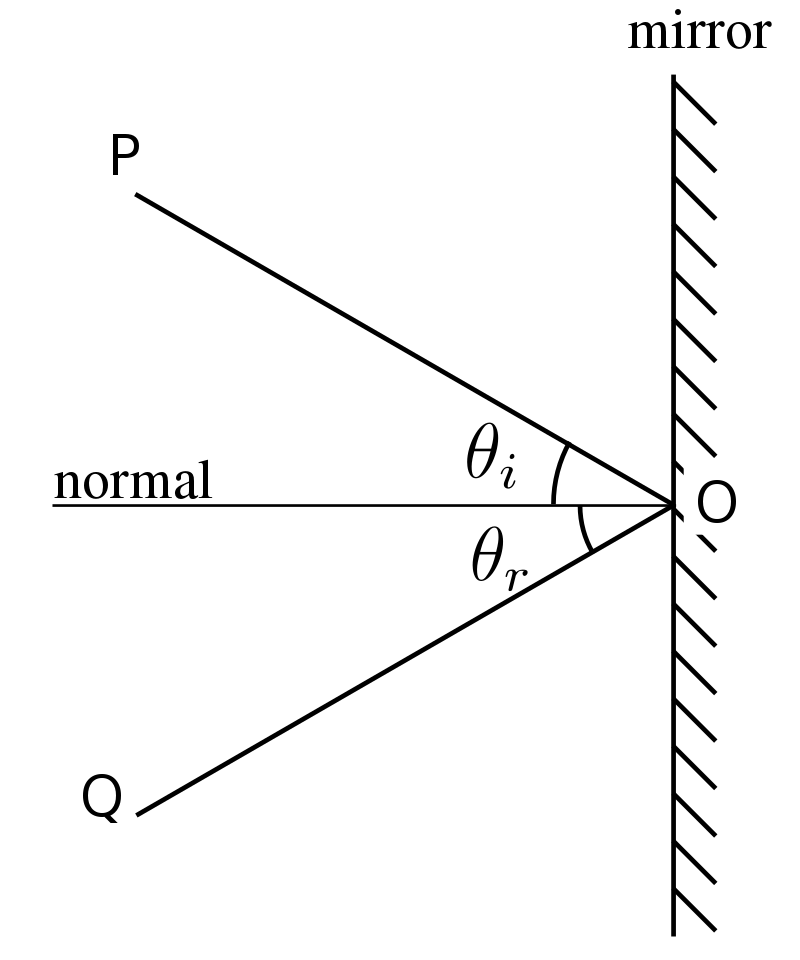
\includegraphics[width=\linewidth]{acoustics/reflection_law.png}
    \captionof{figure}{%
        Specular reflection
    }
    \label{fig:acoustics:reflection_law}
}

If the surface $\surface$ is not perfectly rigid or impenetrable, its behavior is described by the \textit{acoustic impedance}, $\impedence_\surface(f) \in \bbC$.
%\sidenote{\textbf{acoustic impendence} measures the opposition that an acoustic system presents to the acoustic pressure}.
Analytically, it is defined as relation between sound pressure and particle velocity at the boundary.
It consists of a real and imaginary part, called respectively acoustic \textit{resistance} and \textit{reactance}.
The former can be seen as the part where energy is lost, while the latter as the part where energy is stored.
% It measures the portion of energy absorbed by the surface and the incident acoustic wave.
% describes the relation between pressures of the incident arriving waveform and the reflected wave

\newthought{The reflection coefficient} $\reflCoeff$ can be derived by the acoustic impedance
for plane waves, \ie/ under assuming a far-field regime between source, receiver and surface,.
\begin{center}
    \textit{It measures the portion of energy absorbed by the surface
    \\and the incident acoustic wave.}
\end{center}
Analytically, it is defined as  \cite{kuttruff2016room,pierce2019acoustics}
\begin{equation}
    \reflCoeff(f, \theta) = \frac{\impedence_\surface(f)\cos{\theta} - \impedenceAir(f)}{\impedence_\surface(f)\cos{\theta} + \impedenceAir(f)}
    ,
\end{equation}
where $\impedence_\surface(f)$ and $\impedenceAir(f)$ are the frequency-dependent impedance of the surface and the air respectively,
and $\theta$ is the angle of incidence.

\textsc{The absorption coefficient} is typically used instead in the context of \GA/ and the audio signal processing.
It comes from following approximations~\citeonly{savioja2015overview}.
(i) The energy or intensity of the plane wave\sidenote{%
    since it is the square magnitude of the acoustic pressure, the phase information is lost.
}, is considered instead of the acoustic pressure;
(ii) dependency on the angle of incidence is relaxed in favor of the averaged quantities;
(iii) local dependency on frequencies is relaxed in favor of a frequency-independent scalar or at most a description per octave-band.
This assumption are motivated by the difficulty of measuring the acoustic impedance
and the possibility to compute an equivalent coefficient a posteriori

Therefore, it is customary to use the absorption coefficient, defined as
\begin{equation}
    \absCoeff(f) = 1 - \abs{\bar{\reflCoeff}(f)}^2
    ,
\end{equation}
where $\bar{\reflCoeff}$ is the reflection coefficient averaged over the angles $\theta$.

\marginpar{%
    \footnotesize
    The word echo derives from the Greek 'echos', litterarly ``sound''.
    In the folk story of Greek, Echo is a mountain nymph whose ability to speak was cursed:
    she only able to repeat the last words anyone spoke to her.
}\newthought{Echoes are specular reflections} which stand out in terms of energy strength or timing~\citeonly{kuttruff2016room}.
Originally this term used to indicate sound reflections which are subjectively noticeable as a separated repetition of the original sound signal.
These can be heard consciously in outdoor scenario, such as in mountain. However, they are less noticeable to the listener in close rooms.
In~\cref{ch:acoustics:subsec:rir} a proper definition of echoes will be given with respect the temporal distribution of the acoustic reflection.



\subsection{Diffusion, Scattering and Diffraction of Sound}
Real-world surfaces are not ideally flat and smooth; they are rough and uneven.
Examples of such surfaces are coffered ceilings, faceted walls, raw brick walls as well as the entire audience area of a concert hall.
When such irregularities are in same order of the sound wavelength, \textit{diffuse reflections} is observed.

In the context of \GA/, the acoustic ray associated to a plane-wave can be though as a bundle of rays traveling parallel.
When it strikes such a surface, each individual rays are bounced off irregularly, creating \textit{scattering}:
a number of new rays are created, uniformly distributed in the original half-space.
The energy carried by each of the outgoing ray is angle dependent and it
is well modeled thought the \textit{Lambert's cosine law}, originally used to describe optical diffuse reflection.

The total amount of energy of this reflection may be computed a-priori
knowing the \textit{scattering} coefficient proper of the surface material.
Alternatively, it can be derived a-posteriori with the \textit{diffuse coefficient}, namely the ratio between
the specularly reflected energy over the total reflected energy.

\textit{Diffraction waves} occurs when the sound confronts the edge of a finite surfaces, for instance around corners or through door openings.
This effect is show in~\cref{fig:acoustics:diffraction}
\marginpar{%
    \centering
    \footnotesize
    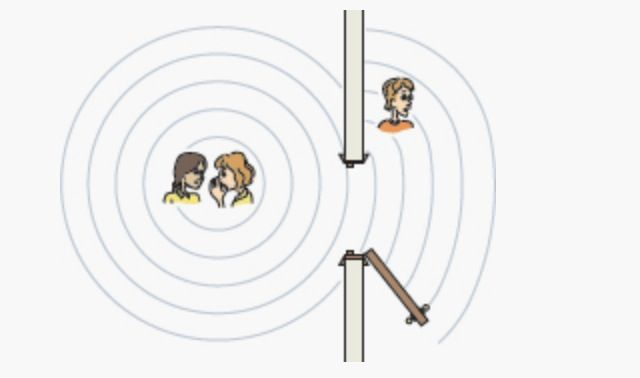
\includegraphics[width=\linewidth]{acoustics/sound_diffraction.jpg}
    \captionof{figure}{%
        Sound Diffraction effect.
    }
    \label{fig:acoustics:diffraction}
}
At first the sound wave propagates spherically from the source.
Once it reaches the reflector with apertures, the wave is diffracted, \ie/ bended, behind it.
It is interesting to note that the diffraction waves produced by the semi-infinite reflector edge
allow the area that is ``behind'' the reflector to be reached by the propagating sound.
This physical effect is exploited naturally by the human auditory system to localize sound sources.

% -----------------------------------------------------------------------------

\section{Room Acoustics and Room Impulse Response}\label{ch:acoustics:sec:rir}
Room acoustics concerns with acoustic waves propagating in air enclosed in a volumes with a set of surfaces
(walls, floors, etc.), from which an incident wave may be interact as described in \cref{ch:acoustics:sec:reflection}.
In this context, a
\begin{center}
    \textit{\emph{room} is a physical enclosure containing the medium and has boundaries limit the sound propagation.}
\end{center}

\textsc{Mathematically} the sound propagation is described by the wave equation~\eqref{eq:acoustics:wave}.
By solving it, the \AIRdef/\sidenote{\ATFdef/ in the Fourier transform of the \AIR/}
from a source to a microphone can be obtained.
In the context of room acoustics, it is commonly referred to as \RIRdef/, usually to put attention of
on the geometric relation between reflections and the geometry of the scene.
In this thesis the two terms will be used indistinctly.

\subsection{The Room Impulse Response}\label{ch:acoustics:subsec:rir}
It is a fundamental concept of this dissertation and it is where physical room acoustic
(Green's function/Solution of wave equation) and indoor audio signal processing meets.
From now on, we well adopt an signal processing perspective and
\begin{center}
\textit{The \RIR/ is a causal time-domain filter that accounts for the whole indoor sound propagation
from a source to a receiver}
\end{center}
\cref{fig:acoustics:rir} provides a schematic illustration of the shape of a \RIR/ in comparison with measured one.
\begin{figure}[h]
    \centering
    \begin{minipage}[b]{.5\textwidth}
        \centering
        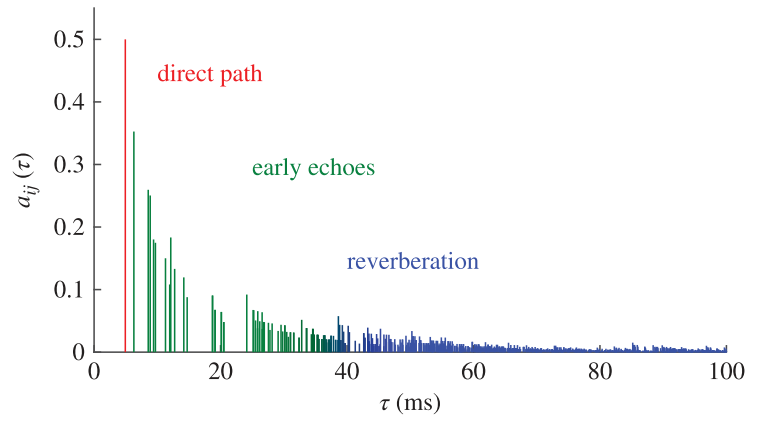
\includegraphics[width=\linewidth]{acoustics/rir_schematic.png}
    \end{minipage}%
    \begin{minipage}[b]{.5\textwidth}
        \centering
        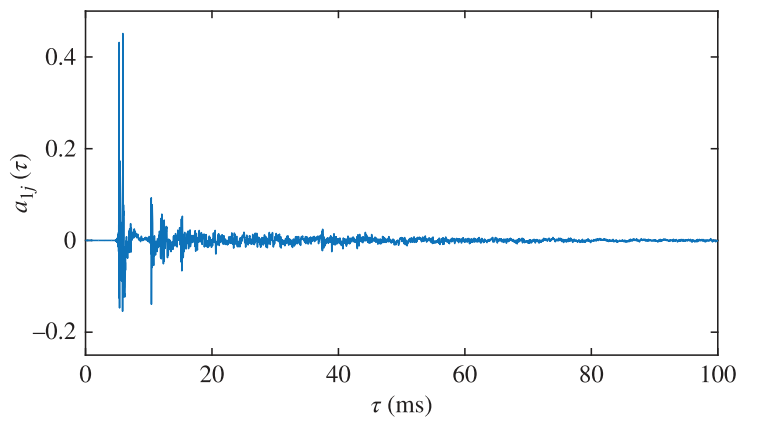
\includegraphics[width=\linewidth]{acoustics/rir_measured.png}
    \end{minipage}
    \caption{Schematic illustration of the shape of an \RIR/ and the first 100 ms of a measured one.}
    \label{fig:acoustics:rir}
\end{figure}

\RIRs/ usually exhibits common structure.
Based on the consideration in~\cref{ch:acoustics:sec:reflection},
they are commonly divided into three components \citeonly{kuttruff2016room}:

\begin{equation}\label{eq:acoustics:rir_full}
\rir(t) = h^d(t) + h^e(t) + h^l(t)
,
\end{equation}
where
\begin{description}
    \item[Direct path] $h^d(t)$ is the line-of-sight contribution of the sound wave.
    This term coincides with the spike modeled by the free-field propagation\sidenote{\cfr{The free-field Green's function, \ie/~\cref{eq:acoustics:greenFreeTime})}}.
    \item[Echoes or Early Refelction] are included in $h^e(t)$ comprising few disjoint reflections coming typically from room surfaces.
    They are usually characterized by sparsity in the time domain and greater prominence in amplitude.
    This first reflections are typically specular and are well modeled in general by the \ISM/\sidenote{\cfr{\cref{subsec:acoustics:ism}}}.
    \item[Later Reverberation] or simply \textit{reverberation} $h^l(t)$ collects many reflections occurring simultaneously.
    This part is characterized by a diffuse sound filed with exponentially decreasing energy.
\end{description}
This three components are not only ``visible'' when plotting the \RIR/ against time,
but they are characterized by different perceptual features, as explained~\cref{ch:acoustics:sec:perception}.

To conclude with, let $s(t)$ be the source signal, sound received is
\begin{equation}
    x(t) = (\rir \conv s)(t)
    ,
\end{equation}
where the symbol $\conv$ is the convolution operator.

A part for certain simple scenarios, computing \RIRs/ in closed forms is a cumbersome task.
Therefore numerical solver or approximation model are used instead.

\subsection{Simulating Room Acoustics}\label{sec:acoustics:simulators}
There are two main categories: geometric and wave-based methods~\cite{habets2006room, savioja2015overview}.
\begin{description}
    \item[wave-based] aims at solving the wave equation numerically, while
    \item[geometric] methods make some simplifying assumption about the wave propagation:
    they typically ignore the \textit{wave} behavior of the sound, choosing much lighter models such as \textit{ray}s or \textit{particle}s.
\end{description}

\newthoughtpar{Wave-based Methods}.
% description
These are iterative methods that divide the 3D bounded enclosure into a grid of interconnected nodes
--- mechanical unit with simple degree of freedoms.
For instance, the
\FEMf/ divide the space into small volume elements smaller of the sound wavelengths, while
\BEMf/ divide only the boundaries of the space are divided into surface elements.
These nodes interact with each other according to the math of the wave equation.
Unfortunately, at high frequencies, the elements must be very small, so their number increases, so the computational complexity increases.
This methods allow to create grid with denser interconnection where required.
\\The \FDTDf/ method replace the derivatives in the wave equation, with its discrete approximation, \ie/ finite differences.
The space is divided into a regular grid, where the changes of a quantity (air pressure or velocity) is computed over time at each grid point.
\DWMf/ methods are a subclass of \FDTD/ often used in acoustics problem.

\begin{figure}[t]
    \label{fig:acoustics:fdtd}
    \centerfloat
    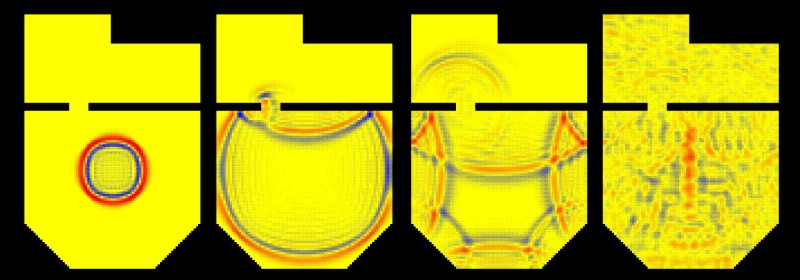
\includegraphics[width=.8\paperwidth]{acoustics/simulator_dwg.jpg}
    \caption{Simulation of Sound propagation at four consecutive timestamps using the \DWM/ technique.
    A short, sharp, impulsive sound fired into the larger of two rooms causes a circular wavefront to spread out from the sound source.
    The the wave is reflected from the walls and part of it passes through a gap into the smaller room.
    In the larger room, interference effects are clearly visible;
    in the smaller room, the sound wave has spread out into an arc, demonstrating the effects of diffraction.
    A short while after the initial event, the sound energy has spread out in a much more random and complex fashion.
}
\end{figure}

\begin{figure}[t]
    \label{fig:acoustics:fdtd}
    \centering
    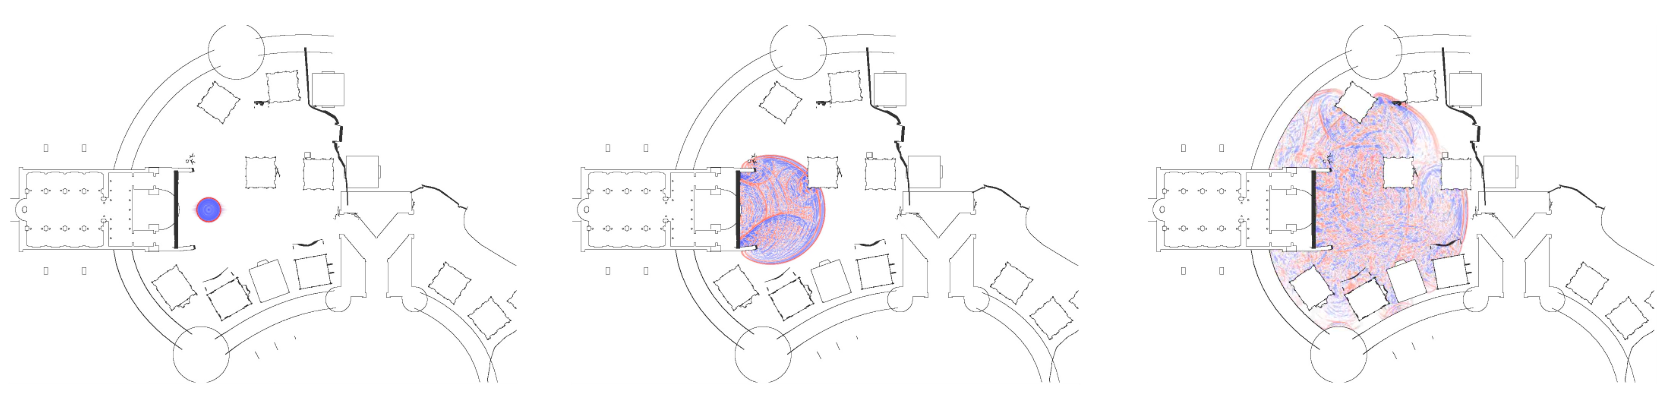
\includegraphics[width=\textwidth]{acoustics/wave-simulation_fdtd.png}
    \caption{Sound propagation at three consecutive timestamps using the \FDTD/-based \textit{Triton} simulator from Microsoft}
\end{figure}

\textsc{The main drawback of these methods} is  discretisation problem:
less dense grid may simplify too much the simulation, while denser grid increase the computational load.
Moreover, in order to achieve good simulation, their require delicate definitions of the boundaries condition and
their complex impedances, parameters not always available in the literature.
\\\textsc{On the other hand} these methods inherently account for many effects such as reflection, diffusion, diffraction and interferences.
In particular by simulating the low-frequencies components of the \RIR/, they are able to well approximate \textit{room modes}
\sidenote{
    Room modes have the effect of amplifying and attenuating specific frequencies in the \RIR/,
    and produce much of the subjective sonic ``colour'' of a room.
}
Reproducing and studying modes is of vital importance
for evaluating acoustic of rooms, such as concert hall, and recording studios or when producing musically pleasing reverbs.

Above all, \DWMf/ are usually preferred\cite{valimaki2016more}: they run directly in the time domain, requiring easier implementation;
and they exhibits a natural huge level of parallelism
\sidenote{each individual node in the grid
(in number of thousands or millions) can be updated without synchronization,
leading to an massive computational reduction}.

\newthoughtpar{Geometric metods}
\marginpar{For a detailed discussion about geometric acoustic methods, please refer to \cite{Savioja2015goemetric}}
They can be grouped into \textit{stochastic} and \textit{deterministic} approaches.
They typically compute the reflection path(s) between the source and the receivers,
assuming that the wave behaves like a particles and a ray carrying the acoustic energy around the scene.

\newthought{Stochastics} are approximate by nature.
They are based on statistical modeling of the \RIRs/ or approximation via Monte Carlo methods.
The formers writes statistical signal processing models based on prior knowledge,
such as energy envelopes and probability distribution of the \RIR/ in regions of time-frequency domain  \cite{Badeau2019common}.
The latters randomly and repeatedly subsample the problem space, recording samples which fulfil some correctness criteria, and discarding the rest.
By combining the results from multiple samples, the probability of an incorrect result is reduced, and the accuracy is increased.
Typically the trade-off between quality and speed is straightforwardly adjusted by choosing the number of samples.

The most common is the \textit{ray-tracing}\cite{Kulowski1985algorithmic} or \textit{diffuse rain}\cite{Schroeder2007fast, Heinz1993binaural, Wabniz2010}

\newthought{Ray-tracing}.
Modeling of waves as discrete particles.
Great success in the field of computer graphics for modeling reflection of light.
The assumption that rays and waves are interchangeable is good for high frequencies.
For low frequencies, where the wavelength are of the same order of the wall surface, it may leads to strong approximation error:
interferences and diffractions effects are not taken into account at these frequencies\cite{Savioja2015goemetric}.

This simulation technique models the propagation by a series of discrete rays that are traced around the room.
Each ray trajectory is reflected in a random direction every time it hits a wall and its energy is scaled according to the wall absorption, air absorption and distance attenuation).
The process of tracing a ray is continued until the ray’s energy falls below a predefined threshold.
At each reflection, the ray's energy over frequency, its time and angle of arrival are recorded in histogram, namely a
\textit{directional time-frequency-energy map} of the room’s diffuse sound field for a giver receiver location.
This map is then used as prior distribution for drawing random set of impulses which are used to form the \RIR/.

\newthought{Deterministic} methods.
the most popular is the Allen and Barkley's \ISMf/\cite{allen1979image}.
It accurate traces the exact direction and the timing of the main reflections' paths.

For a 3D shoebox with rigid walls, it is able to produce an exact solution to the wave equation.
It models only specular (perfect) reflections, ignoring diffuse and diffracted components.
For this is only approximate inexactly arbitrary enclosures and the late reflections, which is predominantly diffuse.

The naive implementation reflects the sound source against all surfaces in the scene, resulting in a set of image sources. Then, each of these image sources is itself reflected against all surfaces
For these reasons, the image-source method is only suitable for early reflections, and is generally combined with a stochastic method to find the late part of an impulse response
For higher order of reflection (\~20), the algorithmic complexity explodes becomes impractical.
For these reasons, the image-source method is only suitable for early reflections, and is generally combined with a stochastic method to find the late part of an impulse response (IR).

\newthought{Hybrid Methods}
As discussed above, the image-source method is accurate for early reflections, but slow for longer responses.
The ray tracing method is by nature an approximation, but produces acceptable responses for diffuse field.
The waveguide method models physical phenomena better than the geometric methods, but is expensive at high frequencies.
This limitation corresponds into three regions in the Time-Frequency representation of the \RIR/.
As depicted in~\cref{fig:acoustics:rir_regions},
\begin{itemize}
    \item in the time domain, a transition can be identified between the early vs. late reflection, corresponding to the validity of the deterministic vs. stochastic models;
    \item and in the frequency domain, between geometric and wave-based modeling.
\end{itemize}

By combining all three models, accurate broadband impulse responses can be created,
but for a much lower computational cost than would be possible with any individual method.
However, this is possible provided that the time- and frequency-domain
\textit{crossover point} are respected and the level of each component is scaled accordingly.

\marginpar{%
    \centering
    \footnotesize
    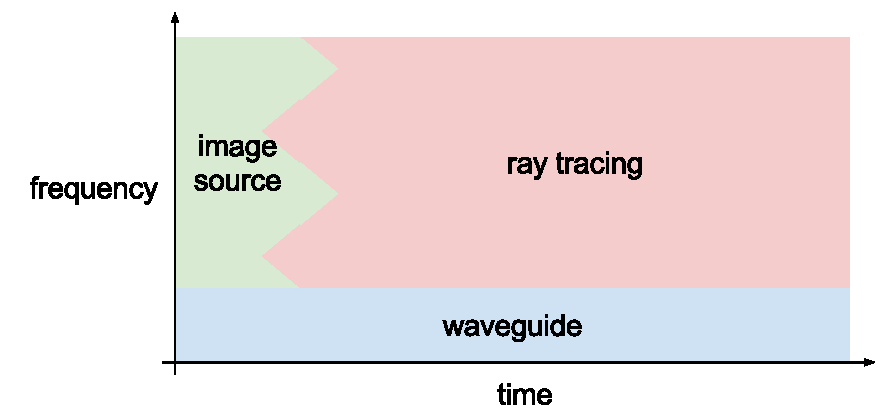
\includegraphics[width=\linewidth]{acoustics/rir_regions.pdf}
    \captionof{figure}{%
    Time-Frequency profile of reverberation Adapted from \cite{Badeau2019common, Wayverb}.
    }
    \label{fig:acoustics:rir_regions}
}

The crossover point in the time domain is called \textit{transition time} or \textit{mixing time}.
It identifies the moment after which reflections are so frequent that they form a continuum and, because the sound is partially absorbed by the room surfaces at every reflection, the sound level decays exponentially over time \cite{Badeau2019common}
This point define the cross-fade between the deterministic and the stochastic process.
Notice, that the latter will record both specular and diffuse reflections.

The crossover point in the frequency domain is called \textit{Schroeder's frequency}, splitting the
spectrum of the \RIR/ into a region with a few isolated modes and one where they can be threated as a
continuous random process, called respectively the \textit{resonant} and \textit{even} behaviors.
This point define the cross-fade between the geometrical and wave-based model.

Each simulator has its own way to compute and implement this crossover points.

\subsection{The Method of Images and the Image Source Model}\label{subsec:acoustics:ism}

The \textit{Method of Images} is a mathematical tool for solving certain class of differential equations subjected to boundary conditions.
By assuming the presence of a ``mirrored'' source, certain boundary condition are verified greatly facilitating the solution of the original problem.
This methods is widely used in many fields of physics, and interestingly with specific application to Green's functions.
Its application to acoustic was originally proposed by Allen and Berkley in \cite{allen1979image} and it is know as the \ISMf/.
Now it is probably the most used technique for \RIR/ simulation due its conceptual simplicity and its flexibility.

The \ISM/ is based on purely specular reflection and it assumes that the sound energy travels around a scene in “rays”.

In the appendix of \cite{allen1979image}, the authors also proved that this method produce a close solution to the one the Helmholtz's equation.
The image solution of a rectangular enclosure
rapidly approaches an exact solution of the wave equation as the walls of the room become rigid.

\newthought{Locally, the Image Source} defines the interaction of the propagating sound with the reflectors.
It is based on the observation that when a ray is reflected, it spawns a secondary source “behind” the boundary surface.
This additional source is located on a line perpendicular to the wall, at the same distance from it as the original source, as if the original source has been “mirrored” in the surface.
In this way, the each wavefront that arrives to the receiver from each reflection off the walls as the direct path received from an equivalent (or image) source.

Assumption:
\begin{itemize}
    \item sound source and receiver as points in a rectangular cavity
    \item purely specular reflection paths between a source and a receiver
    \item This process is simplified by assuming that sound propagates only along straight lines or rays
    \item Rays are perfectly reflected at boundaries
\end{itemize}

When a rigid wall is present, it represents a boundary condition to the wave equation, namely to have zero normal velocity vector.
Assuming a lossless reflection, \ie/ $\absCoeff = 0$, a way to satisfy the boundary condition is to assume
an additional sound source, called the \textit{image source}, placed symmetrically to the main source on the far side of the wall.

Moreover, as discussed in~\cref{ch:acoustics:sec:reflection}, such a surface generates specular reflection.

The model is depicted in~\cref{fig:acoustics:image_model}.
A sound source is located in $\positionSource$ near a reflecting wall.
At the receiver position $\positionMicrophone$ two signals arrives: the one coming directly from $\positionSource$

A ray which is reflected from several boundaries is represented by a “higher-order” image-source,
which has been mirrored in each of those boundaries\cite{Kuttruff}. In this way, the

All sources, original and image, emit the same impulsive source signal at the same time. The total impulse response (i.e. sound pressure against time) is found by summing the signals from each source, delayed and attenuated appropriately depending on the distance between that source and the receiver, which is equivalent to the length of the specular reflection path. The frequency response of the signal from each image source will additionally be modified depending on the characteristics of each boundary in which that source was reflected.

In the real world, not all energy is perfectly reflected at a boundary.
Some energy will be randomly diffused in non-specular directions.
The image-source model is not capable of modelling this phenomenon, though this is not particularly problematic.
Consider that, once scattered, sound energy cannot become un-scattered.
The conversion from incoming energy to scattered energy is unidirectional, so repeated reflections cause the ratio of scattered to specular energy to increase monotonically.
Kuttruff shows that, though the earliest reflections may be largely specular, after a few reflections the large majority of sound energy becomes diffuse [2, p. 126].
This suggests that the image model should be used only for very early reflections, where most energy is not scattered, and a secondary model used to compute late, diffuse reflections.
In Wayverb, the image model is used for early reflections, and stochastic ray-tracing is used for the diffuse tail.
The combination of the two models is described in the Hybrid Model section.

%%%%%%%%%%%%%%%%%%%%%%%%%%%%%%%%%%%%%%%%%%%%y
\section{Perception and Some Acoustic Parameters}\label{ch:acoustics:sec:perception}
In the previous sections we have analyzed reverberation from a purely physical point of view.
However in many applications it is important to correlate physical measurements to subjective and perceptual acoustical qualities.
This will be important in order to define evaluation scenarios later in this thesis.
\sidenote{
    \footnotesize
    \textbf{\textit{Cite Sacks about perception}}
}
\subsection{The Perception of the \RIR/ elements}
It is commonly accepted that the \RIR/ components defined in~\cref{ch:acoustics:subsec:rir} play rather separate roles in the perception of sound propagation.

\newthought{The Direct Path} is the delayed and attenuated version of source signal itself.
It coincides with the free-field sound propagation and, as we will see in~\cref{chap:mirage}, it reveals the direction of the source.

\newthought{Early Reflections and Echoes} are reflections which are by nature highly correlated with to the direct sound.
They convey a sense of geometry which modify the general perception of the sound:
\begin{description}
    \item[The Precedence Effect] occurs when two correlated sounds are perceived as a single auditory event~\cite{wallach1973precedence}.
    This happens usually when they reach the listener with a delay within $\SI{5}{\ms}$ to $\SI{40}{\ms}$.
    However, the perceived spatial location carried by the first-arriving sound is preserved suppress the perceived location of the lagging sound.
    This allows human to accurately localize the direction of the main source, even in presence of its strong reflections.
    \item[The Comb Filter Effect] indicates the change in timbre of the perceived sound, named \textit{coloration}.
    This happens when multiples reflections arrive with periodic patterns and some constructive or destructive interferes may arise.
    Such phenomena can be well modeled with a comb filter \cite{barron1971subjective}..
    \item[Apparent Source Width] is the audible impression of a spatially extended sound source~\cite{griesinger1997psychoacoustics}.
    By the presence of early reflection, the perceived energy increases, providing the impression that a source sounds larger than its optical size.
    \item[Distance and Depth Perception] provides to the listener cues about the source location.
    While the former refers to the spatial range, the latter relates the source to the auditory scene as a whole~\cite{kearney2012distance}.
    A fundamental cue for distance perception is the \textit{direct-to-reverberant ratio} ($\DRR$)\sidenote{\cfr~\cref{ch:acoustics:subsec:drr}},
    \ie/ the ratio between the direct path ration and the remain portion of the \RIR/.
    Regarding the depth perception, early reflection are the main responsible.
    In the context of virtual reality, correct modeling of these quantities is essentials in order to maintain a coherent depth impression~\cite{kearney2012distance}.
\end{description}

\newthought{The Late Reverberation} in room acoustics is indicative of the size the environment and the materials within~\cite{valimaki2016more}.
It provides the \textit{listener envelopment}, \ie/ the degree of immersion in the sound field~\cite{griesinger1997psychoacoustics}.
This portion of the \RIR/ is mainly characterized by the sound diffusion, which depend on the surfaces roughness.

\subsection{Mixing time}
Perceptually, it define the instant when the reverberation cannot be distinguished from that of any other position of the listener in the room.
Analytically,  the
\begin{center}
    \textit{\emph{mixing time} is the instant that divides the early reflections from the late reverberation in a RIR},
\end{center}
And it is represented in Equation 2.47 by the symbol Tm.
Due to this, it is an parameters important also in the context of \RIRs/ synthesis as it defines cross-over point for room acoustics simulator using hybrid methods~\citeonly{savioja2015overview}\sidenote{\cfr~\cref{sec:acoustics:simulators}}.

\subsection{Reverberation Time}
The \textit{reverberation time} measures the time that takes the sound to ``fade away'' after it ceases.
In order to quantify it, acoustics and in audio signal processing use the \textit{Reverberation Time at 60 dB}, \ie/
\begin{center}
    \textit{the $\RT$, the time after which the sound energy relatively dropped by 60 dB.}
\end{center}
It depends on the size and absorption level of the room (including obstacles), but not on the position of specific position of the source and the receiver.
Real measurements of \RIRs/ are affected by noise.
As a consequence, it is not always possible to consider a dynamic range of 60 dB,
\ie/ the energy gap between the direct path and the ground noise level.
In this case, the $\RT$ value must be approximated with other methods.
A practical approach is presented in~\cref{ap:rir:sec:rt60}.

By knowing the room geometry and the surfaces acoustics profiles,
it is possible to use the empirical \textit{Sabine's equation}:
\begin{equation}
    \RT
    \approx 0.161 \frac{V_{\text{TOT}}}{\sum_l \absCoeff_l S_l} \hspace{1em} [\si{\second}]
    ,
\end{equation}
where $V_{\text{TOT}}$ is the total volume of the room $[\si{\metre^3}]$ and $\absCoeff_l$ and $S_l$ are the
absorption coefficient and the area $[\si{\metre^2}]$  of the $l$-th surface.

\subsection{Direct-to-Reverberant ratio and Critical Distance}\label{ch:acoustics:subsec:drr}
\begin{center}
    \textit{The \emph{direct-to-reverberant ratio} ($\DRR$) quantifies the power of direct against indirect sound~\cite{zahorik2002direct}.}
\end{center}
It varies with the size and the absorption of the room, but also with the distance between the source and the receiver according to the curves
depicted in~\cref{fig:acoustics:drr}
\marginpar{%
    \centering
    \footnotesize
    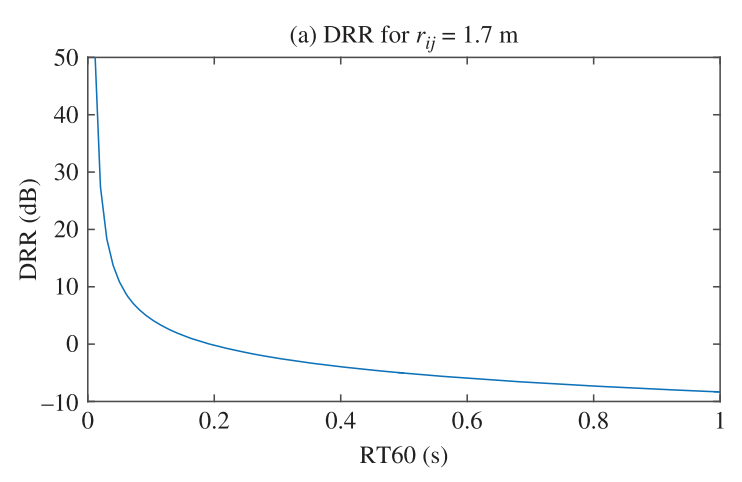
\includegraphics[width=\linewidth]{acoustics/drr_rt60.png}
    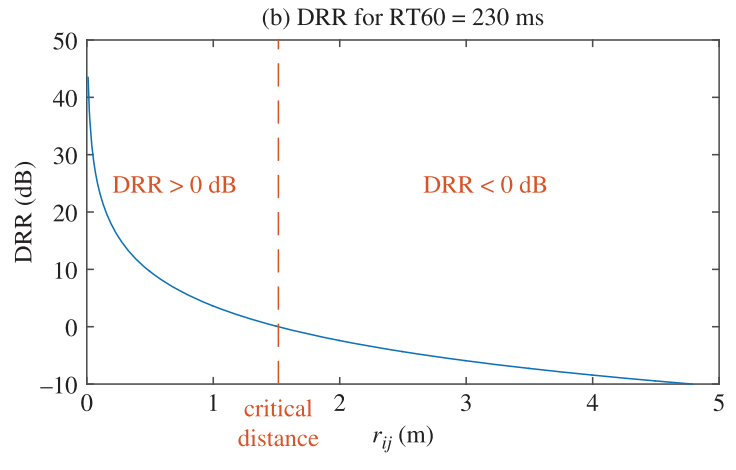
\includegraphics[width=\linewidth]{acoustics/ddr_dist.png}
    \captionof{figure}{%
        DRR as a function of the RT60 and the source distance rij based on Eyring’s formula (Gustafsson et al., 2003).
        These curves assume that there is no obstacle between the source and the microphone, so that the direct path exists.
        The room dimensions are the same as in Figure 3.1.
    }
    \label{fig:acoustics:drr}
}
% A proper analytical definition will be provided in the next chapter.
% % The $\DRR$ at the mth microphone in each microphone configuration was calculated using the method
% % \begin{equation}
% %     \DRR_\idxMic = 10 \log_{10}{\frac{
% %         \sum_{n=-\infty}^{\infty} \kparen{h^d_{ij}(n)}^2}%
% %         {\sum_{n=-\infty}^{\infty} \kparen{h^e_{ij(n)}}^2}}
% %         = 10 \log_{10}{\frac{
% %             \sum_{n=-\infty}^{\infty} \kparen{h^d_{ij}(n)}^2}%
% %             {\sum_{n=-\infty}^{\infty} \kparen{h^e_{ij}(n)}^2}}
% % \end{equation}
The distance beyond which the power of indirect sound becomes larger than that of direct sound is called the \textit{critical distance}.

These quantities represent an important parameter to assert the robustness of audio signal processing methods,
since they basically measure the validity of the free-field assumption.

% Similarly, one can define the \textit{direct-to-early ratio} ($\DER$), which is the power of direct sound divided by the remaining power in the first ??c samples (defined above),
% quantifies the modification of the power spectrum of the signal induced by early echoes.
%  It is low when the microphone and/or the source is close to an obstacle such as a table or a window, and higher otherwise.
%  The DRR and the direct-to-early ratio are not systematically reported when describing experiments in the literature,
%   yet they are as important as the RT60 to characterize multichannel mixtures

% \chapter{Signal Processing and Audio Inverse Problem}\label{chap:processing}


\section{Signal Model}
This section is about the signal model


\subsection{Multichannel Mixing Process}

\subsection{Time-Frequency Analysis and Synthesis}

\subsection{Artificial Mixtures}

\subsection{Impulse Response Models}
\newthoughtpar{Acoustic and Room Impulse Response}

\newthoughtpar{Acoustic and Room Transfer Functions}

\newthoughtpar{Steering Vectors}

\newthoughtpar{Relative Transfer Functions}

\newthoughtpar{Full-Rank Covariance Models}

%%%%%%%%%%%%%%%%%%%%%%%%%%%%%%%%
\section{Audio Inverse Problems}
\newthoughtpar{Forward vs Inverse Problem}

\subsection{General Processing Scheme}
General Processing Pipeline

\subsection{Some Audio Inverse Problems}
\begin{enumerate}
    \item sound source separation and enhancements
    \item sound source localization
    \item microphones calibration
    \item channel estimation
    \item room geometry estimation
    \item acoustic echo estimation
\end{enumerate}
\newthoughtpar{Evaluation}

%%%%%%%%%%%%%%%%%%%%%%%%%%%%%%%%
\section{Taxonomy through dichotomies}
%% acoustics %%
\newthoughtpar{Single-Channel vs. Multichannel}
\newthoughtpar{Point vs. Diffuse Sources}
\newthoughtpar{Directonal vs. Onmidirectional Recordings}
\newthoughtpar{Diffuse vs. Measurements Noise}
%% processing %%
\newthoughtpar{Natural vs. Artificial Mixtures}
%% pipeline %%
\newthoughtpar{Problem vs. Model}
\newthoughtpar{Synthesis vs. Abstaction}
%% problems %%
\newthoughtpar{Separation vs. Enhancement}
%% models %%
\newthoughtpar{end2end vs. 2step}
end2end: from data to (feature to) target
\\2-step: (from data to features) + features to target

\newthoughtpar{Knowledge-based vs. Learning-based}
\begin{itemize}
    \item Bottom-up vs Top-down information processing
    \item Knowledge-based: specialized signal processing and mathematical algorithms informed by knowledge;
    \item Learning-based: machine learning usually trained in supervised fashion.
\end{itemize}

\newthoughtpar{Supervised vs. Unsupervised}
\newthoughtpar{Machine Learning vs. Deep Learning}

% % II. Estimation
% \begin{fullwidth}
% \part{Acoustic Echo Retrieval}\label{pt:estimation}
% \end{fullwidth}
% \parttoc[n]
% \chapter{Acoustic Echo Retrieval}\label{chap:estimation}
\openepigraph{Signal, a function that conveys information about a phenomenon.
$[\dots]$ Consider an acoustic wave, which can convey acoustic or music information.}{R. Priemer, \textit{Introductory Signal Processing}}
\vspace{-2.5em}
\newthought{Synopsis}  blabla

\section{Problem Formulation}
The \AERdef/ problem consists in estimating the echoes' timings (or delays) $\kbrace{\tau_r}$ and attenuations (or gains) $\kbrace{\alpha_r}$.
In this context the echoes are considered the early reflections component of the \RIR/, modeled as
\begin{equation}
    \echoModelFreq
    .
\end{equation}
The term \AER/ is not an established name for such problem and depending on the field of research and the prior knowledge available, it can be referred to with different name.
In fact \AER/ can be seen as general case of Time of Arrivals Estimation or a instance of Acoustic Channel Estimation and Shaping, and Spike Retrieval and Onset Detection.
As opposed to \AER/, the task of Time of Arrivals Estimation, is only focused in estimating the echos' timings $\kbrace{\tau_r}$.
The only knowledge $\kbrace{\tau_r}$ is sufficient for typical application of related to Sound Source Localization and Room Geometry Reconstruction.
Moreover knowing $\kbrace{\tau_r}$, the attenuations $\kbrace{\alpha_r}$ can be estimated in a subsequent phase using closed-from equations~\citeonly{condat2015cadzow}.
Time of Arrivals Estimation is sometimes called Time Delays Estimation, when the origin of time is taken \wrt/ the first \TOA/ and not when sound emission.
\AER/ may be confused with Time Delay Estimation.
\AER/ may be confused with Acoustic Echo Cancellation which refers to the problem of estimating and removing...

\section{Taxonomy on \AER/ methods}

In general, we can identify four main categories which differ on whether the transmitted signal is know or not and on whether the estimation of the \RIR/.

\dichotomy{Active vs. passive approaches}.
When the input/transmitted source signal is known, then the scenario is said \textit{active}.
This type of approaches uses one or more loudspeaker to probe the environment and one or more microphones to record the propagated probe sound.
This type of methods falls into the big categories of \textit{deconvolution problem} since a ``clean'' reference signal is used to deconvolve the observed one.
Two are the main advantages of these approaches. First, this methods can be used in single-microphone scenario.
Second, with proper probe signal, a good estimation of the \RIR/ can be achieved.
Instead, passive or blind approaches are source agnostic.
To decouple environment from source signal, they leverage either on prior knowledge on the source signal or by comparing the signals received at two (or more) spatially-separated microphones.

\dichotomy{RIR-agnostic vs. RIR-based approches}.
As opposed to \textit{direct}, \textit{2-step} methods estimate the echoes' properties after estimating the (full or partial) \RIR/(s).
By modeling the early part of the \RIR/ as collection of Dirac, solving the \AER/ problem can be seen as solving two subsequent tasks:
\RIR/ estimation followed by echoes extraction.
The former can be seen as an instance of Channel Estimation problems, while the latter as a spike retrieval, pick picking or onset detection.

The latter is more challenging since, in general settings, theoretical ambiguities make this problem unsolvable~\citeonly{xu1995least, subramaniam1996cepstrum, tong1998multichannel}.
\\Instead of estimating the full acoustic impulse response, other methods estimate it partially using assumptions derived by the application.
It is the case of Impulse Response Shaping or Shortening.
In context of room acoustics, they aim to reduce the late reverberations allowing some early reflections which are perceptually useful~\citeonly{betlehem2012efficient}.
\\Direct methods instead try to surpass the challenging task of estimating the full \RIR/ and tuning peak-picking methods, and set-up an end-to-end framework.
May extract other information.

\newthought{Channel Equalization or Inverse Filtering}, is a particular case of channel estimation.
Here the goal is to estimate an equalization filter, which is the inverse of the channel impulse response, rather than the estimation of the channel impulse response itself.
This equalization filter is then applied to the received signal in order to extract the transmitted one\sidenote{\textit{Beamforming} or \textit{Spatial Filtering} can be seen as in this sense}.
In general estimating the equalization filter can be easier or more difficult than estimate the direct filter~\sidenote{If the channel impulse response is assumed to be minimum phase, the problem becomes trivial.}.
\citeonly{neely1979invertibility}, shows that even if the \RIR/ is perfectly known, its direct inversion is not straightforward.
Several techniques were investigated to alleviate an exhaustive review of Room Response Equalization can be found in~\citeonly{cecchi2018room}.

\newthought{Channel Shaping} is another approach similar to the one of channel equalization \citeonly{krishnan2015robust, vairetti2017scalable}.

Given the above definition, we can now review so \AER/ methods presented in the literature.

\section{Literature Review}

\subsection{Active and RIR-based method}
In this categories falls all the methods that first attempt for a ``good'' estimation of \RIRs/ for which the transmitted signal is known.
The echoes are identified and peaks in the estimated \RIRs/ and ad-hoc techniques are used to identify them.

\newthought{The \RIR/ Estimation step} is typically modeled as a deconvolution problem whose performances depends on the type of transmitted signal.
When the transmitted signal is arbitrary, several methods were developed to measure real \RIRs/.
Since the \RIR/ identifies the room response to a perfect impulse, one can measured by producing an impulse sound, \eg/ finger snap, a clap, piercing a ballon, or a gun shot.
Even though this methods are still used in acoustic measurement, they show clear limitation in term of reproducibly and safety.
Moreover a perfect impulse is difficult to approximate.
Instead, modern computational technique are used, involving speaker and microphone and computing the deconvolution (or cross-correlation) between an known emitted signal and the recorded output.
\\The \MLSdef/ technique was first proposed by Schroeder~\citeonly{schroeder1979integrated} and it is based on the excitation of the acoustical space by a periodic pseudo-random signal, called \MLS/.
The RIR is then calculated by circular cross-correlation between the measured output and the original \MLS/ signal.
This method was further improved in order to achieve better \RIR/ estimation in~\citeonly{dunn1993distortion,aoshima1981computer}.
Unfortunately this technique introduces several distortion artifacts which yield to spurious peaks and components in the estimation and it is sensible to the harmonic distortion introduced by the playback device, \eg/ the loudspeakers.
\\To overcome this issue, the \ESSdef/ technique introduced by Farina~\citeonly{farina2000simultaneous,farina2007advancements}.
The probe signal is the \ESS/ signal, \aka/ \textit{chirp signal}, which benefit of the following properties:
the signal span a certain frequency range; it is self-orthogonal, namely it compress into Dirac's impulse during autocorrelation; and its Fourier inverse is known in closed form.
The last property allows the user not to record and invert the probe signal.
The reader can find a review of the presented techniques in~\citeonly{szoke2019building}
\sidenote{This technique has many other propreties. On can refer to the Farina's tutorial~\cite{farina2007advancements} and this Python tutorial} %\href{https://medium.com/@baranov.mv/how-i-was-listening-to-a-sine-sweep-all-day-long-294c374995f6}}.

\mynewline
Sometimes the transmitted signal is known, but one of the above technique cannot be used.
In this scenario, \RIR/ estimation problem needs to be addressed as a more general deconvolution problem, typically solved through optimization methods~\citeonly{lin2006bayesian}.
This approaches are well studied and can be solved using standard Linear Least Squares with closed-form solution.
However, in case of narrowband signal (\eg/ speech or music) or low SNR, these problems become ill-conditioned and prior knowledge about the \RIR/ bay improve the estimation~\citeonly{boooh}.

\newthoughtpar{Echo Retrieval from RIR}
As discussed through~\cref{pt:background}, acoustic echoes can be identified as peaks in the early part of the \RIR/.
In general, such peak are not necessarily positive, thus to better visualize the \textit{echogram}\citeonly{kuttruff2016room}, namely $\rir = \magnitudeOf{\rir}$, or the energy envelop~\citeonly{schroeder1979integrated} are used instead%
\sidenote{The energy envelope typically computed as the magnitude of the analytic signal computed with the Hilbert transform.}.
Provided a good estimation of it, this peaks location and amplitudes could be extracted manually by experts.
However, even in ideal scenario, the automation of this process and the correct identification such quantities are not straightforward tasks.
As showed in \citeonly{tukuljac2018mulan}, since the arrival time of each reflection is not necessarily multiple of the sampling grid, their true location (and amplitudes) are blurred by spurious peaks.
Moreover the harmonic distortion due to the non-ideal source-receiver coupling can creates spurious spikes as well.
This issue which is referred to as \textit{basis mismatch} in the \textit{compressed sensing} community reveals the strong limitation of simple \RIR/ peak-pinking.
Although it can be alleviated by increasing the sampling frequency, it is bound to occurs in practice.
And small errors of echoes timing estimation yield to significant differences in echo-based application~\cite{defrance2008finding}.
\\The existing methods can be dichotomized into three broad categories: on-gird and off-grid approaches.
The methods belonging to the former group are the most used in practice but advance technique are used to coupe with the above mentioned issue.
~\citeonly{kuster2008reliability, crocco2017uncalibrated, remaggi2016acoustic, defrance2008detecting, bello2005tutorial, cheng2016attack, defrance2008detecting, annibale2012geometric, kelly2014detecting, usher2010improved}.
The most straightforward way is to deploy iterative and adaptive thresholding algorithm on the followed by robust and manually tuned peak finders ~\citeonly{kuster2008reliability, crocco2017uncalibrated}.
In the work~\citeonly{remaggi2016acoustic}, based on a algorithm presented in\citeonly{naylor2006estimation}, peaks are clustered according to changes in the phase slope.
Similar techniques are used in the field of music onset detection, where edge-detection wavelet filters~\citeonly{bello2005tutorial} or the attach-decay pattern~\citeonly{cheng2016attack} are used to detect event onset.
Other methods consist in peaks are selected considering the \RIR/ Kurtosis In~\citeonly{usher2010improved}.
\\By noticing that the reflection in the \RIRs/ exhibit similar shape of the direct path, the author of~\citeonly{defrance2008detecting} first proposed the use of Matching Pursuit to identified such shapes.
Here the direct sound part was used as an atom in a matching pursuit algorithm.
Unfortunately, in its pure form, matching pursuit is unsuitable for \RIRs/ because of the non-stationary nature of the reflection affected by frequency dependent characteristic of the room absorption material.
In order to improve the detection, \citeonly{kelly2014detecting} extents this approach employing Dynamic Time Warping to account for the non-uniform compression, dilation and concurrency of the early reflection.
Nevertheless, the idea of exploiting the direct path component to isolate the source-receiver coupling and thus identified first prominent reflection through deconvolution was used in~\citeonly{annibale2012geometric}.
This is known also as matching filter or direct-path compensation.
\\Alternatives approaches, detect the echo timings in other signal representation.
In \citeonly{vesa2010segmentation}  the echoes are localized in the time frequency domain using the cross-wavelet transform based on the early work~\citeonly{guillemain1996characterization, loutridis2005decomposition}.
Curiously the recent works~\citeonly{ristic2013detection,pavlovic2016multifractal} uses (multi-)fractal analysis to detect echoes in the time-frequency domain.

\mynewline
All the above mentioned works aims at detecting echoes on the sampling grid.
In order to coupe with the pathological issues of this approach, off-grid framework can be used, \eg/~\citeonly{condat2013robust}.
This approach can be related to other classical \ML/ estimation problem, which consist in selecting the model which is most likely to explain the observed noisy data.
In this categories fall other classical spectral estimation technique, \eg/ \MUSIC/~\citeonly{loutridis2005decomposition}, \ESPRIT/~\citeonly{roy1986esprit}, which are fast but statistically suboptimal.
The method presented in \citeonly{condat2013robust} focuses on the general problem of estimating a finite stream of Dirac pulses from uniform, noisy, lowpass-filtered samples.
This problem can be reformulated as a matrix denoising problem, from which the echoes location and amplitudes can be retrieved in closed-from.
Although this method reach statistical optimality in \ML/ sense, the exact knowledge of number of Diracs needs to be known in advance.
If this number is unknown or approximated, huge errors in the estimation are observed.
This consist in a huge drawbacks since a priori the exact number of echoes is difficult to know and false-positive spikes are present even in clear \RIRs/.

\mynewline
That have being said, \AER/ is far from trivial and solved even on clean \RIR/ estimate.
It is crucial to note that, for every TOA estimator, a practical trade off exists between the number of missed TOAs and the number of spurious TOAs wrongly selected.
This trade-off is only partially dependent by the SNR since, also for clean received signals, many factors can provide spurious peaks.
For instance, side lobes due to finite signal bandwidth, echo distortions due to frequency dependent attenuations and coalescing peaks due to close TOAs can affect peak estimation.
This fact is often a source of unavoidable outliers that make the robustness of subsequent steps in room estimation a delicate and very important issue.
A way to overcome this issues is to overestimate the echoes in the \RIR/ by including some false-positive observation and further prune them.

\newthought{Peak Disambiguation}
\textit{Echo labeling} or \textit{\TOA/ Disambiguation} is the task of assign acoustic echoes to different image source or reflectors.
Many methods are been proposed in the context of \SSL/~\citeonly{scheuing2006disambiguation, zannini2010improved}, microphone calibration~\cite{parhizkar2014single,salvati2016sound}
and \RooGE/~\citeonly{filos2011robust, antonacci2012inference, dokmanic2013acoustic, crocco2014towards, jager2016room, el2017time}.
In the context of \SSL/, the disambiguation is typically performed in the \TDOAs/ which are makes them more prone to error since higher precision is required\sidenote{%
For instance, at $\SI{48}{kHz}$ a \TDOA/ from the same wavefront between a sensor pair $\SI{40}{cm}$ apart and a source $\SI{2.6}{m}$ away, takes a very small value of $\SI{4.46}{\samples}}.



\begin{itemize}
    \item \citeonly{el2017time} root paper
    \begin{itemize}
        \item \citeonly{dokmanic2013acoustic}
        \item \citeonly{antonacci2012inference, filos2011robust}
        \item \citeonly{jager2016room} using graph
        \item For SSL as described in el2017time \citeonly{scheuing2006disambiguation, zannini2010improved}
    \end{itemize}
    \item \citeonly{crocco2014towards} root paper
    \item \citeonly{antonacci2012inference}
    \item \citeonly{salvati2016sound,parhizkar2014single}
\end{itemize}


\subsection{Active and RIR-agnostic method}
EM and DOA estimation \citeonly{jensen2019method, saqib2020estimation} root paper

using autocorrelation / acoustic cameras
\citeonly{chen2006time} for review Typically the time-difference-of-arrival (TDOA) of the direct path is estimated with the aim to localize a speaker or an interfering sound source.
\citeonly{crocco2014towards}
\citeonly{o2010automatic} and used later in \citeonly{o2008imaging}
autocorrelation \citeonly{al2019early}


\subsection{Passive and RIR-based method}
FIR BSI SIMO

The root in blind channel identification can be found is~\citeonly{sato1975method}
Since then, many algorithms have been proposed
Since it was recognized that the problem can be solved in the light of only SOS[2], the focus ofthe blind channel identification research has shifted to SOS methods, behind which, the motiva- tion is the potential for fast convergence. There is a rich literature on SOS blind channel identification. Many batch methods have had good success to some extent, such as the subspace (SS) algorithm [3], the cross relation (CR) algorithm [4], [5], the least squares component normalization (LSCN) algorithm [6], the linear prediction based subspace (LP-SS) algorithm [7], and the two-step maximum likelihood (TSML) algorithm
see ~\citeonly{tong1998multichannel} for a review.
\begin{itemize}
    \item subspace method: The key idea is that the channel (or part of the channel) vector is in a one- dimensional subspace of either the observation statistics or a block of noiseless observations.
    These methods, which are often referred to as subspace algorithms, have the attractive property that the channel estimates can often be obtained in a closed form from optimizing a quadratic cost function
    Pro: closed-from identification.
    Cons: as they rely on the property that the channel lies in a unique direction (subspace), they may not be robust against modeling errors.
    especially when the channel matrix is close to being singular.
    The second disadvantage is that they are often more computationally expensive.
    \item maximum likelihood method y, unlike subspace based approaches, the ML methods usually cannot be obtained in closed form.
\end{itemize}

root papers \citeonly{tukuljac2018mulan}
here multiple passive sensors.
To the best of the authors’ knowledge, all existing methods in blind channel identification rely on the discrete-time model
Blind Channel Estimation~\citeonly{xu1995least, tong1998multichannel}
\begin{itemize}
    \item Subspace methods
    \item Cross Relation methods
    \item Sparsity based cross-relation
    \item Maximum likelihood
\end{itemize}

BCE for RIR estimation. root paper \citeonly{crocco2016estimation}
\citeonly{tong1994blind,lin2007blind,lin2008blind,kowalczyk2013blind,crocco2015room,crocco2016estimation}
\begin{itemize}
    \item introduction of the cross relation~\citeonly{tong1994blind}. SIMO can be formulated as a eigenvalue problem - least square minimization
    \item anchor constrain and non negative~\citeonly{lin2007blind}
    \item bayesian learning for lambda~\citeonly{lin2008blind}
    \item spit Bergam methods~\citeonly{kowalczyk2013blind}. which is known to be robust to back- ground noise.
    \item iterative weighted l1 constrain~\citeonly{crocco2015room} and improved in~\citeonly{crocco2016estimation}.
    to better balance sparsity penalty and sparsity constraints.
    \item Kalman \citeonly{qi2019broadband}
\end{itemize}

BSI for RIR, root paper ~\citeonly{qi2019broadband}
\begin{itemize}
    \item Subspace mathods
    \item Linear Prediction Coding
    \item Cross Relation
    \item RTF with oversampling~\citeonly{koldovsky2015sparse}
\end{itemize}

BCE for RIR estimation, root paper \citeonly{kowalczyk2013blind}
\begin{itemize}
    \item SIMO-BSI which exploits spatial differences between multiple microphone signals, has received significant attention as it does not require any assumption about the source signal and can be formulated as an adaptive algorithm~\citeonly{huang2003class}
    \item in \citeonly{chen2006time} to outperform crosscorrelation-based techniques, such as generalized crosscorrelation (GCC), for source localization in noisy and reverberant environments. At the cost of complexity.
\end{itemize}

Under this perspective, \RTF/ estimation techniques can be used.
As mentioned in~\cref{subsec:processing:rtf}, the \RTF/ can be
RTF estimation in the special case $h_i = 1$
In particular scenarios, when microphone is close to one source, the RIR at another microphone RTF estimation methods can be used~\citeonly{koldovsky2015spatial}.

limitation of this methods:

% Although they rely on sparsity-enforcing regularizers, the filters are strictly-speaking non- sparse in practice, due to the sinc kernel (Fig. 1). This general bottle-neck in compressed sensing has been referred to as basis mismatch and was notably studied in [28]. In particular, the true peaks of the filters do not correspond to the true echoes (Fig. 1), even for N to inf. Though, most existing methods rely on peak-picking [18, 5].
\begin{itemize}
    \item For the same reason, these methods are fundamentally on-grid, namely, they can only output echo locations which are integer multiple of the sampling period 1/Fs. This pre- vents subsample resolution, which may be important in applications such as room shape reconstruction from audio signals [3].
    \item These methods strongly rely on the knowledge of the length L of the filters. However, due to the sinc kernel (Sec. 2.1.1), the true filters are always infinite.
    \item The dimension of the search space isML-1, which is much larger in practice than the actual number 2MK of unknown variables. This makes the methods computationally demanding and sometimes intractable for large filter lengths (typically in the tens of thousands for acoustic
\end{itemize}

After it, peak picking

\subsection{Passive and RIR-agnostic method}
Note that the real channel is not perfectly non-negative since the Dirac pulses, corresponding to the walls reflections, typically fall off the grid of samples resulting in sinc functions. Despite this slight mismatch between theoretical assumptions and real data, the position of the estimated peaks reproduces the positions of the ground truth peaks with remarkable precision.
This are also off-grid methods
\begin{itemize}
    \item MULAN \citeonly{tukuljac2018mulan}
    \item Blaster \citeonly{di2020blaster}
    \item Audio cameras - beamforming~\citeonly{sun2011joint}
\end{itemize}

% Approaches
% \begin{itemize}
%     \item assuming ideal propagation
%     \begin{description}
%         \item[M=2, Cross-correlation approaches]
%         \item[M=2, Generalized Cross-correlation approaches]
%         \item[M=2, LMS-type adaptive]
%         \item[Sensor Fusion] SRP-PHAT
%     \end{description}
%     \item assuming reverberant path
%     \begin{description}
%         \item[Adaptive Eigenvalue decomposition]
%     \end{description}
% \end{itemize}

% Is the transmitted signal known?
% \begin{description}
%     \item[Yes] Active Channel Estimation
%     \begin{itemize}
%         \item Deconvolution followed by Peak Picking methods
%         \begin{description}
%             \item[Deconvolution]
%             \begin{itemize}
%                 \item Regression and Deconvolution
%                 \item Informed Deconvolution (Sparsity)
%                 \item RTF estimation in the special case $h_i = 1$
%                 \item RIR estimation \citeonly{Farina}
%                 \item cross correlation
%             \end{itemize}
%             \item[Peak Picking]
%             \begin{itemize}
%                 \item Iterative Thresholding (Crocco)
%                 \item Condat - Sinc Denoising
%                 \item Defrance - Matching Pursuit
%                 \item Remmagi, Naylor
%                 \item Onset detection
%                 \item Kurtosis
%                 \item Autocorrelation
%                 \item Matched filter / Direct Path compensation
%                 \item Geometry-based
%                 \item DTW - Kelly
%                 \item Multifractals analysis
%                 \item Time-Frequency representation (Wavelet) - Vesa and Lokki
%             \end{itemize}
%         \end{description}
%         \item Jesper Jensen
%         \begin{itemize}
%             \item EM and DOA
%             \item \cite{crocco2014towards}
%             \item Active Acoustic Cameras
%             \item autocorrelation \citeonly{al2019early}
%         \end{itemize}
%     \end{itemize}
%     \item[No]. Do we have prior Knowledge?
%     \begin{description}
%         \item[Yes] Statistics methods
%             \item 2nd order
%             \item ML
%             \item leglaive
%         \item[No] Is it on grid? Does it estimate the full channel? Require peak picking?
%             \begin{description}
%                 \item[Yes] On grid Blind Method
%                     \begin{itemize}
%                     \item subspace method
%                     \item cross-relation methods
%                     \end{itemize}
%                 \item[No]
%                 \begin{itemize}
%                     \item MULAN
%                     \item Blaster
%                     \item Audio camera
%                 \end{itemize}
%             \end{description}
%     \end{description}
% \end{description}

\section{Data and Evaluation}

\subsection{Datasets}
Syntethic RIRs

Real RIRs

\subsection{Metrics}
The metrics used in \AER/ depend on the application and the methods used to estimate the echoes.
It following that two types of metrics can be identified.

\newthoughtpar{BCE metrics}
For application related to channel estimation, \eg/ speech enhancement, typically both echoes timing and amplitudes are required.

\newthoughtpar{Information Retrival Metrics}
aoeu

% \section{as (sparse) \RIR/ estimation}
% \begin{itemize}
%     \item[def] estimation of the whole channel acoustic channel
%     \item[methods] Signal know \vs/ unknown. statistical methods \vs/ blind method
% \end{itemize}

% \subsection{Other echo-related parameters estimation}
% \newthought{\TDOA/ estimation}
% \begin{itemize}
%     \item[def] estimation of the the difference of the direct path
%     \item[methods] Cross-correlation
% \end{itemize}

% \newthought{Echo Density Estimation}

% \newthought{$\RT$ and $\DRR$ estimation}

% \section{Acoustic Echo Estimation is}

% \begin{itemize}
%     \item Acoustic Echo Retrieval definition
%     \item Acoustic Echo Retrieval scope and placement in the signal processing pipeline
%     \item Acoustic Echo Retrieval characteristic
% \end{itemize}

% \section{Echoes in the Time, Frequency and Cepstral domains}
% \begin{itemize}
%     \item Time domain processing
%     \item Frequency domain processing
%     \item Correlation processing
%     \item Cepstral processing
% \end{itemize}


% \section{Related Works}
% \subsection{Active vs. Passive echoes estimation}

% \subsection{Knowledge-based vs. Data-driven}
% \begin{itemize}
%     \item Knowledge-driven (Physic-driven)
%     \begin{itemize}
%         \item Channel (RIR) estimation and Echoes pruning - Crooco and Dokmanic
%         \item TDOA estimation (multipath) - Benesty
%         \item Spikes Retrieval - Condat
%     \end{itemize}
%     \item Data-driven
%     \begin{itemize}
%         \item GLLiM
%         \item Deep Leaning echo estimation
%     \end{itemize}
% \end{itemize}

% \subsection{end-2-end vs 2-steps approaches}

% AER\\
% eRTF + AER

% Pruning methods

% \section{Related Works}

% \subsection{AER as a RIR Estimation problem}
% \todo{summarize Crocco's presentation}

% TX signal: known vs. not known
% \\TX signal not known: statistical methods and blind methods

% \subsection{AER as a Spike Estimation problem}


% \subsection{Virtually-supervised and Data Augmentation}


% \section{Data and Metrics}
% \subsection{Spike-based metrics}
% \chapter{\library{Blaster}: Knowledge-driven Acoustic Echo Retrieval}\label{ch:blaster}
\openepigraph{
    My beautiful astronaut//
    With an impulsive world//
    A twisted scientist!}{Venetian Snares, \textit{1000 Years}}

\vspace{-2.5em}
\newthought{Synopsis} \marginpar{%
\footnotesize
\textbf{Keywords:} Blind Channel Identification, Super Resolution, Sparsity, Acoustic Impulse Response.
\\\textbf{Resources:}
\begin{itemize}
    \item \href{https://doi.org/10.1109/ICASSP40776.2020.9054647}{Paper}
    \item \href{https://gitlab.inria.fr/panama-team/blaster}{Code}
    \item \href{https://hal.archives-ouvertes.fr/hal-02469901}{Open-access paper with supplementary material}
    \item \href{https://sigport.org/documents/blaster-grid-method-blind-and-regularized-acoustic-echoes-retrieval}{Slides}
    \item \href{https://youtu.be/rPaqZJIfpKo}{Presentation}
\end{itemize}
} \synopsisChBlaster

\mynewline
The material presented in this chapter was previously published in~\cite{di2020blaster} and results from a collaboration with my colleague Clement Elvira whose domain of expertise is in the \CDdef/ framework, while my expertise lies in the audio and acoustic signal processing and modeling aspects.
The section dedicated on the presentation of the \CD/ framework applied to \AER/ is extracted from the related publication and it is written with the help of my colleague.
Here we briefly commented and expanded it and some attention is paid in highlighting the motivation behind it.
Finally, this chapter recalls the main findings of the paper, while bringing additional insights in the existing models for \AER/.

\section{Introduction}
\label{sec:blaster:intro}
% %Striking introducing sentence
% As deeply discussed so far, the temporal structure of the \RIRdef/ plays a central role in room acoustics and audio signal processing.
% % First echo is noise
% It is the result of multiple (indirect) sound propagation paths due to specular and diffuse reflections on the room's surfaces, leading to reverberation~\citeonly{Wang2011}.
% In such conditions, the perceived sound quality is often considered degraded and it is common to observe a detrimental decrease of performance as reverberation increases for applications such as speech recognition~\citeonly{Yoshoka2012} or music information retrieval~\citeonly{Barthet2010}.
% % or music virtual reality~\citeonly{DeMan2017}. %to observe a detrimental decrease of performances with reverberation. as well as music virtual reality~\citeonly{DeMan2017}.

% % Second echo is information
% On the other hand, RIRs contain very rich geometrical information about the acoustic scene.
% %which is independent from the source signal itself.
% %In contrast with well-consolidated methods,
% Recent \textit{echo-aware} works have shown that the knowledge of the timing of early reflections may boost performance in many audio signal processing applications,
% from dereverberation~\citeonly{Wu2006,Lin2008} to sound localization~\citeonly{ribeiro2010,DiCarlo2019} and separation~\citeonly{Dokmanic2015a, Scheibler2017}.
% Moreover, it allows joint estimation of the receivers' positions~\citeonly{Salvati2016}, the reflective surfaces~\citeonly{Antonacci2012} and consequently the geometry of the room~\citeonly{Dokmanic2013, crocco2017uncalibrated}.
% % or acoustic impedance of surfaces~\citeonly{Antonello2014, Bertin2016}.
% % beamforming \citeonly{dokmanic2015raking},
% % such as for speech enhancement \citeonly{Wu2006}, source localization \citeonly{ribeiro2010}, source separation \citeonly{Scheibler2017} and dereverberation \citeonly{Lin2009}
% % which are common pre-processing steps for many applications \citeonly{Gannot2017}

% \AERdef/ consists in estimating the properties of the early (strong) acoustic reflections only in multi-path environments, and sometimes referred to as time delay estimation~\citeonly{chen2006time}.
Let us recall from~\cref{ch:estimation} some knowledge-based methods addressing \AER/.
Some existing methods rely on a known source signal~\citeonly{park2017compressive,jensen2019method}.
In contrast, when multiple receivers attend an unknown single source, \AER/ can be seen as an instance of \SIMOdef/ \BCEdef/ problem, \ie/ estimating the filters entailing an unknown input and an observed output of a system.
A common approach for solving \AER/ in the context of \SIMO/-\BCE/ is to first blindly estimate a discrete version of the acoustic channels using the so-called cross-relation identity~\citeonly{xu1995least, crocco2016estimation}.
The location of the echoes are then chosen among the strongest peaks with ad-hoc peak-picking techniques.
Such methods are generally \emph{on-grid} in the sense that the estimation relies on a fixed grid of time samples and \textit{a priori} chosen filter lengths.
However, in practice, the true timings of echoes rarely match the sampling grid, thus leading to pathological issues called basis-mismatch in the field of compressed sensing.
To circumvent this issue, the authors of~\citeonly{tukuljac2018mulan} proposed to leverage the framework of finite-rate-of-innovation sampling to make one step towards off-grid approaches.
Despite promising results in the absence of noise and with synthetic data, the quality of the estimation highly relies on the choice of a good initialization point.

\mynewline
Of particular interest in the proposed approach is the recently proposed framework of \CDdef/~\citeonly{candes2014towards}.
By formulating an inverse problem as the recovery of a discrete measure over some parameter space, \CD/ has allowed to overcome imaging device limitations in many applications such as super-resolution~\citeonly{candes2014towards} or PALM/STORM imaging~\citeonly{denoyelle2019sliding}.
In this work, we formulate the problem of \AER/ for stereophonic mixtures, \ie/ using only one microphone pair, within the framework of continuous dictionaries.
The resulting optimization problem is convex and thus not prone to spurious minimizers.
The proposed method is coined \emph{\BLASTERdef/} and requires no parameter tuning.
The method is compared to state-of-the art on-grid approaches under various noise and reverberation levels using simulated data.


\section{Signal model}
We consider here the common setup of stereophonic mixtures, that is 2-channel microphone recordings.
Using the notation presented~\cref{ch:processing}, the continuous-time signal recorded at microphone $\idxMic\in\{1,2\}$ reads
\begin{equation}
    \label{eq:blaster:recordedSignal}
    \tilde{\mic}_i(t) = (\tilde{\src} \convCont \tilde{\flt}_i^\star)(t) + \tilde{\nse}_i(t)
\end{equation}
where $\convCont$ denotes the (continuous) convolution operator, $\tilde{n}_i$ models some additive noise in the measurement process and $\tilde{\flt}_i^\star$ denotes the \RIRdef/.
In the remainder of this chapter, the superscript $\star$ refers to the requested \ac{RIR}.
Assuming the echo model, the \acp{RIR} read
\begin{equation}
    \label{eq:blaster:def_filter_star}
    \tilde{\flt}_i^\star(t) = \sum_{\idxEch=0}^{\numEchs_i} \alpha_i^{(r)} \delta(t - \tau_i^{(r)}) + \tilde{\varepsilon}_i(t)
\end{equation}
where $\numEchs_i$ is the (unknown) number of echoes.
\\In the noiseless case, that is when $\tilde{\nse}_i = 0$ for $i\in\{1,2\}$, we have the cross-relation identity
\begin{equation} \label{eq:blaster:cross-relation}
    \tilde{\mic}_1 \convCont \tilde{\flt}_2^\star = \tilde{\mic}_2 \convCont \tilde{\flt}_1^\star
\end{equation}
by commutativity of the convolution operator.
\\However, in practice, only sampled versions of the two recorded signals are available.
More precisely, we consider the measurement model introduced in~\cref{ch:processing}:
the incoming signal undergoes a (ideal) low-pass filter $\lowpassfilter$ with frequency support $\kintervcc{\sfrac{-\Fs}{2}}{\sfrac{\Fs}{2}}$ before being regularly sampled at the rate $\Fs$.
We denote $\disRecordedSignal_1,\disRecordedSignal_2\in\bbR^{2N}$ the two vectors of $2N$ (consecutive) samples and $i\in\{1, 2\}$ by
\begin{equation}
    \label{eq:blaster:measurement-process}
    \disRecordedSignal_i[n] =
    \kparen{\idealLowPassFilter \convDis \contRecordedSignal}\kparen{\frac{n}{\Fs}}
    \qquad
    \forall n \in\{0, \dots, 2N-1\}
    .
\end{equation}

\section{Background on on-grid blind channel estimation}\label{sec:blaster:background}
We now select and elaborate more on some of the methods mentioned in~\cref{subsec:estimation:bce} concerning optimization approaches for \FIR/-\SIMO/-\BCE/.
Therefore, the following methods operate on discrete-time signal, which are denoted without the tilde according to the notation presented in~\cref{ch:processing}.
Starting from the identity \cref{eq:blaster:cross-relation}, the common \SIMO/-\BCE/ cross-relation framework aims to compute $\contFilter_1, \contFilter_2$ solving the following problem in the discrete-time domain~\citeonly{lin2007blind}:
\begin{equation}
    \label{eq:blaster:xrel_toepl}
    \disFilterHat_1, \disFilterHat_2
    =
    \kargmin_{\disFilter_1, \disFilter_2}
    \;
    \tfrac{1}{2}
    \kvvbar{
        \scrT(\disRecordedSignal_1) \disFilter_2
        -
        \scrT(\disRecordedSignal_2) \disFilter_1
    }_2^2
    +
    \lambda
    \kvvbar{
        \bfh
    }_1
\end{equation}
where
\begin{itemize}
    \item  $\disRecordedSignal_i$ and $\disFilter_i$ are the discrete, sampled version of $\contRecordedSignal_i, \contFilter_i$ respectively,
    \item $\scrT(\disRecordedSignal_i)$ is the $(2N+L-1) \times L$ Toeplitz matrix (built as shown in~\cref{fig:blaster:toeplitz})\marginpar{
        \centering
        \resizebox{\linewidth}{!}{
            

\tikzset{every picture/.style={line width=0.75pt}} %set default line width to 0.75pt

\begin{tikzpicture}[x=0.75pt,y=0.75pt,yscale=-1,xscale=1]
%uncomment if require: \path (0,300); %set diagram left start at 0, and has height of 300

%Shape: Rectangle [id:dp9681290386895156]
\draw   (190,80) -- (280,80) -- (280,120) -- (190,120) -- cycle ;
%Shape: Rectangle [id:dp4105274901835]
\draw  [fill={rgb, 255:red, 208; green, 2; blue, 27 }  ,fill opacity=1 ] (190,30) -- (200,30) -- (200,40) -- (190,40) -- cycle ;
%Shape: Rectangle [id:dp07108913371302106]
\draw  [fill={rgb, 255:red, 245; green, 166; blue, 35 }  ,fill opacity=1 ] (200,30) -- (210,30) -- (210,40) -- (200,40) -- cycle ;
%Shape: Rectangle [id:dp27992457661326675]
\draw  [fill={rgb, 255:red, 248; green, 231; blue, 28 }  ,fill opacity=1 ] (210,30) -- (220,30) -- (220,40) -- (210,40) -- cycle ;
%Shape: Rectangle [id:dp22621399339540804]
\draw  [fill={rgb, 255:red, 74; green, 144; blue, 226 }  ,fill opacity=1 ] (220,30) -- (230,30) -- (230,40) -- (220,40) -- cycle ;
%Shape: Rectangle [id:dp8143232980428775]
\draw  [fill={rgb, 255:red, 80; green, 227; blue, 194 }  ,fill opacity=1 ] (230,30) -- (240,30) -- (240,40) -- (230,40) -- cycle ;
%Shape: Rectangle [id:dp3194122969586535]
\draw  [fill={rgb, 255:red, 184; green, 233; blue, 134 }  ,fill opacity=1 ] (240,30) -- (250,30) -- (250,40) -- (240,40) -- cycle ;
%Straight Lines [id:da5684493017647214]
\draw    (193,20) -- (247,20) ;
\draw [shift={(250,20)}, rotate = 180] [fill={rgb, 255:red, 0; green, 0; blue, 0 }  ][line width=0.08]  [draw opacity=0] (3.57,-1.72) -- (0,0) -- (3.57,1.72) -- cycle    ;
\draw [shift={(190,20)}, rotate = 0] [fill={rgb, 255:red, 0; green, 0; blue, 0 }  ][line width=0.08]  [draw opacity=0] (3.57,-1.72) -- (0,0) -- (3.57,1.72) -- cycle    ;
%Straight Lines [id:da9066793447166841]
\draw    (290,83) -- (290,117) ;
\draw [shift={(290,120)}, rotate = 270] [fill={rgb, 255:red, 0; green, 0; blue, 0 }  ][line width=0.08]  [draw opacity=0] (3.57,-1.72) -- (0,0) -- (3.57,1.72) -- cycle    ;
\draw [shift={(290,80)}, rotate = 90] [fill={rgb, 255:red, 0; green, 0; blue, 0 }  ][line width=0.08]  [draw opacity=0] (3.57,-1.72) -- (0,0) -- (3.57,1.72) -- cycle    ;
%Shape: Rectangle [id:dp8376347441359862]
\draw  [fill={rgb, 255:red, 208; green, 2; blue, 27 }  ,fill opacity=1 ] (250,90) -- (240,90) -- (240,80) -- (250,80) -- cycle ;
%Shape: Rectangle [id:dp7117636003093408]
\draw  [fill={rgb, 255:red, 245; green, 166; blue, 35 }  ,fill opacity=1 ] (240,90) -- (230,90) -- (230,80) -- (240,80) -- cycle ;
%Shape: Rectangle [id:dp4138379160748573]
\draw  [fill={rgb, 255:red, 248; green, 231; blue, 28 }  ,fill opacity=1 ] (230,90) -- (220,90) -- (220,80) -- (230,80) -- cycle ;
%Shape: Rectangle [id:dp3999938091654833]
\draw  [fill={rgb, 255:red, 74; green, 144; blue, 226 }  ,fill opacity=1 ] (220,90) -- (210,90) -- (210,80) -- (220,80) -- cycle ;
%Shape: Rectangle [id:dp9277683628608865]
\draw  [fill={rgb, 255:red, 80; green, 227; blue, 194 }  ,fill opacity=1 ] (210,90) -- (200,90) -- (200,80) -- (210,80) -- cycle ;
%Shape: Rectangle [id:dp38590620029972567]
\draw  [fill={rgb, 255:red, 184; green, 233; blue, 134 }  ,fill opacity=1 ] (200,90) -- (190,90) -- (190,80) -- (200,80) -- cycle ;

%Straight Lines [id:da7133925241736656]
\draw    (193,70) -- (277,70) ;
\draw [shift={(280,70)}, rotate = 180] [fill={rgb, 255:red, 0; green, 0; blue, 0 }  ][line width=0.08]  [draw opacity=0] (3.57,-1.72) -- (0,0) -- (3.57,1.72) -- cycle    ;
\draw [shift={(190,70)}, rotate = 0] [fill={rgb, 255:red, 0; green, 0; blue, 0 }  ][line width=0.08]  [draw opacity=0] (3.57,-1.72) -- (0,0) -- (3.57,1.72) -- cycle    ;
%Shape: Rectangle [id:dp49856978345829306]
\draw  [fill={rgb, 255:red, 208; green, 2; blue, 27 }  ,fill opacity=1 ] (260,100) -- (250,100) -- (250,90) -- (260,90) -- cycle ;
%Shape: Rectangle [id:dp3235825725633823]
\draw  [fill={rgb, 255:red, 245; green, 166; blue, 35 }  ,fill opacity=1 ] (250,100) -- (240,100) -- (240,90) -- (250,90) -- cycle ;
%Shape: Rectangle [id:dp31123598821243614]
\draw  [fill={rgb, 255:red, 248; green, 231; blue, 28 }  ,fill opacity=1 ] (240,100) -- (230,100) -- (230,90) -- (240,90) -- cycle ;
%Shape: Rectangle [id:dp11900662558381525]
\draw  [fill={rgb, 255:red, 74; green, 144; blue, 226 }  ,fill opacity=1 ] (230,100) -- (220,100) -- (220,90) -- (230,90) -- cycle ;
%Shape: Rectangle [id:dp5949312347675072]
\draw  [fill={rgb, 255:red, 80; green, 227; blue, 194 }  ,fill opacity=1 ] (220,100) -- (210,100) -- (210,90) -- (220,90) -- cycle ;
%Shape: Rectangle [id:dp4169331213844353]
\draw  [fill={rgb, 255:red, 184; green, 233; blue, 134 }  ,fill opacity=1 ] (210,100) -- (200,100) -- (200,90) -- (210,90) -- cycle ;

%Shape: Rectangle [id:dp6629627557025272]
\draw  [fill={rgb, 255:red, 208; green, 2; blue, 27 }  ,fill opacity=1 ] (270,110) -- (260,110) -- (260,100) -- (270,100) -- cycle ;
%Shape: Rectangle [id:dp31604732616257436]
\draw  [fill={rgb, 255:red, 245; green, 166; blue, 35 }  ,fill opacity=1 ] (260,110) -- (250,110) -- (250,100) -- (260,100) -- cycle ;
%Shape: Rectangle [id:dp09107227856524347]
\draw  [fill={rgb, 255:red, 248; green, 231; blue, 28 }  ,fill opacity=1 ] (250,110) -- (240,110) -- (240,100) -- (250,100) -- cycle ;
%Shape: Rectangle [id:dp7267681930473228]
\draw  [fill={rgb, 255:red, 74; green, 144; blue, 226 }  ,fill opacity=1 ] (240,110) -- (230,110) -- (230,100) -- (240,100) -- cycle ;
%Shape: Rectangle [id:dp29680219911700556]
\draw  [fill={rgb, 255:red, 80; green, 227; blue, 194 }  ,fill opacity=1 ] (230,110) -- (220,110) -- (220,100) -- (230,100) -- cycle ;
%Shape: Rectangle [id:dp12926304976478886]
\draw  [fill={rgb, 255:red, 184; green, 233; blue, 134 }  ,fill opacity=1 ] (220,110) -- (210,110) -- (210,100) -- (220,100) -- cycle ;

%Shape: Rectangle [id:dp11163148873105677]
\draw  [fill={rgb, 255:red, 208; green, 2; blue, 27 }  ,fill opacity=1 ] (280,120) -- (270,120) -- (270,110) -- (280,110) -- cycle ;
%Shape: Rectangle [id:dp3773220154233181]
\draw  [fill={rgb, 255:red, 245; green, 166; blue, 35 }  ,fill opacity=1 ] (270,120) -- (260,120) -- (260,110) -- (270,110) -- cycle ;
%Shape: Rectangle [id:dp21547184217790727]
\draw  [fill={rgb, 255:red, 248; green, 231; blue, 28 }  ,fill opacity=1 ] (260,120) -- (250,120) -- (250,110) -- (260,110) -- cycle ;
%Shape: Rectangle [id:dp30710052799291054]
\draw  [fill={rgb, 255:red, 74; green, 144; blue, 226 }  ,fill opacity=1 ] (250,120) -- (240,120) -- (240,110) -- (250,110) -- cycle ;
%Shape: Rectangle [id:dp8950222427502034]
\draw  [fill={rgb, 255:red, 80; green, 227; blue, 194 }  ,fill opacity=1 ] (240,120) -- (230,120) -- (230,110) -- (240,110) -- cycle ;
%Shape: Rectangle [id:dp01705103269779118]
\draw  [fill={rgb, 255:red, 184; green, 233; blue, 134 }  ,fill opacity=1 ] (230,120) -- (220,120) -- (220,110) -- (230,110) -- cycle ;


% Text Node
\draw (167,25.4) node [anchor=north west][inner sep=0.75pt]  [font=\footnotesize]  {$x_{i}$};
% Text Node
\draw (146,95.4) node [anchor=north west][inner sep=0.75pt]  [font=\footnotesize]  {$\scrT( x_{i})$};
% Text Node
\draw (214,11.4) node [anchor=north west][inner sep=0.75pt]  [font=\tiny]  {$2N$};
% Text Node
\draw (291,97.4) node [anchor=north west][inner sep=0.75pt]  [font=\tiny]  {$L$};
% Text Node
\draw (215.5,61.4) node [anchor=north west][inner sep=0.75pt]  [font=\tiny]  {$2N+L-1$};


\end{tikzpicture}

            }
            \captionof{figure}{Graphical representation of the construction of $\scrT(x_i)$ from $x_i$}
            \label{fig:blaster:toeplitz}
            }
    associated to a convolution where $2N$ and $L$ respectively denote the microphone and filter signal lengths,
    \item $\bfh = \klist{h_1^\intercal, h_2^\intercal}$ is the concatenation of the two vectorized discrete filters,
    \item and the $\ell_1$ regularization term is used to enforce sparsity in the estimation, which is consistent with the ``train of impulses'' model for the early part of \acp{RIR} (but not for the tail).
\end{itemize}
This type of problem can be seen as an instance of \LASSO/ problem~\citeonly{tibshirani1996regression}, written in the form:
\begin{equation}\label{eq:blaster:lasso}
    \kargmin_{u} \tfrac{1}{2} \kvvbar{v - Au}_2^2 + \lambda\kvvbar{u}_1
    .
\end{equation}
This type of well-known optimization problem are convex and, despite the non-differentiability of the $\ell_1$-norm, they can be easily tackled by standard optimization tool.
Later, in this section, we show how to express~\cref{eq:blaster:xrel_toepl} as a standard \LASSO/ problem.

\mynewline
The accuracy of estimated \acp{RIR} has been subsequently improved using a priori knowledge on the filters.
In particular, the authors of~\citeonly{lin2007blind} have proposed to use non-negativity constraints to increase robustness to noise and avoid trivial solution.
Therefore, let us define a more general formulation for~\cref{eq:blaster:xrel_toepl}, as follows
\begin{equation}\label{eq:blaster:sota}
    \disFilterHat_1, \disFilterHat_2
    =
    \kargmin_{\disFilter_1, \disFilter_2}
    \;
    \scrJ(\disFilter_1, \disFilter_2) + \scrP(\disFilter_1, \disFilter_2)
    \;\text{s.t.}\;
    \scrC(\disFilter_1, \disFilter_2)
\end{equation}
where $\scrJ(\disFilter_1, \disFilter_2) = \tfrac{1}{2} \kvvbar{\scrT(\disRecordedSignal_1) \disFilter_2 - \scrT(\disRecordedSignal_2) \disFilter_1}_2^2$ is the cost function to optimize.
$\scrP(\disFilter_1, \disFilter_2)$ and $\scrC(\disFilter_1, \disFilter_2)$ are respectively a regularization term used to promote sparse solutions and a constrained set.
Thanks to this formulation, current state-of-the-art approaches can be summarized as in the~\cref{tab:blaster:sota}.

\begin{table}[!h]

    \begin{fullwidth}
        \centering
        \small
        
\begin{tabular}{l|c|c|l}
\toprule
Reference & $ \scrP(h_1,h_2)$ & $ \scrC(h_1,h_2)$ & Note \\
\midrule
\citeonly{tong1994blind}
& \xmark
& $\norm{\mathbf{h}}_2^2 = 1$
& It can be solved as smallest-eigenvalue problem\\

\citeonly{kowalczyk2013blind}
& $ \lambda \norm{\mathbf{h}}_1$
& $\norm{\mathbf{h}}_2^2 = 1$
& Non convex due to the quadratic constraint.\\

\citeonly{lin2008blind}
& $ \lambda \norm{\mathbf{h}}_1$
& $ \abs{h_1[0]} = 1$
& Bayesian framework for learning optimal $\lambda$\\

\citeonly{lin2007blind}
& $ \lambda \norm{\mathbf{h}}_1$
& $ h_1[0] = 1, \mathbf{h} \geq 0$
& \\

\citeonly{aissa2008blind}
&
&
& \\

\citeonly{crocco2016estimation}
& $ \lambda \norm{\mathbf{h}}_1$
& $ h_1[0] = 1, \mathbf{h} \geq 0$
& \\

\bottomrule
\end{tabular}

        \caption{Some state-of-the-art penalties and constraints used in~\cref{eq:blaster:sota}.}
        \label{tab:blaster:sota}
    \end{fullwidth}
\end{table}

\mynewline
The constraint $\disFilter_i[0]=1$ is called an \textit{anchor constraint} and it is used to replace the $\ell_2$-norm while keeping the problem convex.
The non-negativity $\bfh \geq 0$ constraint may not be satisfied due to effects such as measurement process, the filtering in the propagation media or the imperfect frequency response of a microphone.
However, when those effects are common to both channels, they can be viewed as distortions to a common source.
Therefore, the non-negativity assumption seems reasonable for real acoustic environments.
Nevertheless, applications concerning \RooGE/ require just the recovery of lower order reflections, i.e. the sparse portion of the \RIR/.
Likewise works in speech enhancement have proven to work under such assumption, thus proving the effectiveness of this approach, such as in~\citeonly{lin2008blind, yu2011multi}.

\mynewline
On a similar scheme, in~\citeonly{kowalczyk2013blind},~\cref{eq:blaster:xrel_toepl} is solved using an adaptive time-frequency-domain approach while~\citeonly{aissa2008blind} proposes to use the $\ell_p$-norm instead of the $\ell_1$-norm.
Choosing $p < 1$, sparsity is enforced, however the problem become non-convex and ad-hoc optimization technique was proposed.
A successful approach has been presented recently by the authors of~\citeonly{crocco2016estimation}, where the anchor constraint is replaced by an \textit{iterative weighted} $\ell_1$ equality constraint, \ie/, such that at each iteration $z$, $\ktranspose{\bfp^{(z)}}\bfh^{(z)} = 1$.\sidenote{
    Note that when $\bfp^{(z)} = \onesVect$, the constraint returns to the $\ell_1$ penalty.}
In particular, the method is initialized using the solution of \citeonly{lin2007blind} and iterated enforcing sparsity using the solution of the previous problem, that is $\bfp^{(z)} = \hat{\bfh}^{(z-1)}$.
The reader can find a comprehensive review of these methods in~\citeonly{crocco2015room,crocco2016estimation}.

\newthought{The limitation of the discrete-time methods} described above are the followings:
\begin{itemize}
    \item \textit{Basis mismatch}:\marginpar{%
        \centering
        \footnotesize
        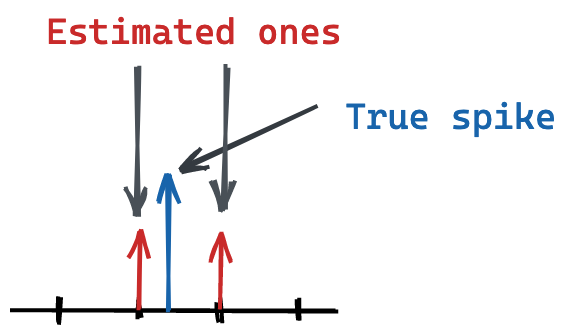
\includegraphics[trim={0 0 0 0},clip,width=\linewidth]{blaster/bodyguard.png}
        \captionof{figure}{%
            Schematics of the \textit{bodyguard effect} affecting on-grid approaches.
            This is true only if $\flt$ is non-negative.
        }
        \label{fig:blaster:bodyguard}
    } As explained in~\cref{subsec:estimation:bce}, the filter are not sparse in practice due to the \textit{basis mismatch}.
    This implies that the peaks of the filter do not necessarily correspond to the true echoes and lead to followings drawbacks.
    As these methods operates fundamentally \textit{on-grid}, they return echoes' timings which are integer multiples of the inverse of $\Fs$.
    \item \textit{Bodyguard effect}.
    In addition to affecting the \AER/ performance, on-grid methods may converge slowly to suboptimal solutions.
    In fact, as shown in~\cref{fig:blaster:bodyguard}, instead of estimating the positive peaks at its true location, two smaller ``bodyguard'' peaks are estimated around it instead.
    The estimation procedure may stop at this point returning two wrong peaks.
    Having smaller coefficients, these peaks may not be selected by the subsequent peak picking technique.
    Alternatively, the optimization procedure may continue, alternating tuning the weights of the two ``bodyguards'', without converging to a solution.
    \item \textit{Computational bottleneck}.
    A way to cope with the above limitations is to increase the $\Fs$.
    However this results into a memory and computational bottleneck as several huge (Toeplitz) matrices need to be built, one for each pair of microphones.
    In addition, this leads to the risk that the optimization problem becomes ill-conditioned.
\end{itemize}

\mynewline
In the following section we will present a novel approach that aims at addressing the above limitations.
It is based on a framework proposed for solving \ac{LASSO} problems for continuous variables, hence the name \ac{CD}.
Before, let us show how to express the on-grid \BCE/ problem proposed by~\citeonly{lin2008blind} (See \cref{tab:blaster:sota}) as a standard \LASSO/ problem.

\subsection{From cross-relation to LASSO}
Integrating the sparse penalty and the constraints proposed in \cref{eq:blaster:sota},
the \BSNdef/ problem proposed reads
\begin{equation}\label{eq:blaster:bsn}
    \disFilterHat_1, \disFilterHat_2
    =
    \kargmin_{\disFilter_1, \disFilter_2}
    \;
    \tfrac{1}{2}
    \kvvbar{
        \scrT(\disRecordedSignal_1) \disFilter_2
        -
        \scrT(\disRecordedSignal_2) \disFilter_1
    }_2^2
    + \lambda\kvvbar{\bfh}_1
    \;\text{s.t.}\;
    \begin{cases}
        \bfh \geq 0\\
        h_1[0] = 1
    \end{cases}
    .
\end{equation}
This cross-relation based optimization problem can be rewritten in the \LASSO/ formulation of~\cref{eq:blaster:lasso} as
\begin{equation*}
    u
    =
    \kargmin_{u}
    \;
    \tfrac{1}{2}
    \kvvbar{ v - B u }_2^2
    + \lambda\kvvbar{u}_1
    \quad\text{s.t.}\quad
    u \geq 0
    ,
\end{equation*}
where
\begin{equation*}
    v = T_2e_1,
    \quad
    u =
    \begin{pmatrix}
        h_1[1:] \\
        h_2
    \end{pmatrix},
    \quad
    A =
    \begin{pmatrix}
        -T_2[:, 1:] & T_1
    \end{pmatrix}
    ,
\end{equation*}
where $T_i = \scrT(x_i)$.
Here we used the light, yet common, Python notation for indexing the matrices and vectors.
The matrix $A$ is typically called \textit{dictionary}.


\section{Proposed approach}

The cross-relation identity~\cref{eq:blaster:cross-relation} ensures that the relation
\begin{equation}
    \idealLowPassFilter
    \ast \contRecordedSignal_1
    \ast  \contFilter_2^\star
    =
    \idealLowPassFilter
    \ast \contRecordedSignal_2
    \ast  \contFilter_1^\star
\end{equation}
holds even during the introduced measurement process, hence
\begin{equation}
    \label{eq:blaster:cross-relation-identity-fourier}
    \fourierTrans(\idealLowPassFilter\ast\contRecordedSignal_1) \cdot \fourierTrans \contFilter_2^\star
    =
    \fourierTrans(\idealLowPassFilter\ast\contRecordedSignal_2) \cdot \fourierTrans \contFilter_1^\star
\end{equation}
where $\fourierTrans$ denotes the \FTdef/ described in~\cref{sec:processing:domains}.
\\In contrast with \SIMO/-\BCE/ methods that operates in the time domain, here we propose to use~\cref{eq:blaster:cross-relation-identity-fourier} in a penalized least-square problem.
Such a formulation in the Fourier domain may even be considered as more convenient since the convolution operator is no longer involved.
While the \FT/ of $\contFilter_i^\star$ can be expressed in closed-form (see~\cref{eq:blaster:closed-form-TF-dirac-N} below), the \FT/ of $\idealLowPassFilter\ast\contRecordedSignal_i$ is not available due to the measurement process.
To circumvent this issue, we consider the \DFTdef/ of $\contRecordedSignal_i$:
\begin{equation}
    \label{eq:blaster:approx-TF}
    \fourierTrans(\idealLowPassFilter\ast\contRecordedSignal_i)
    %(\tfrac{f}{F_s})
    \kparen{\tfrac{k}{2N}F_s}
    =
    X_i[k]
\end{equation}
for all integers  $k \in \{0, \ldots, N\}$, where
\begin{equation}
    \label{eq:blaster:dft-Xi}
    \RecordedSignalDFT_i[k] = \sum_{n=0}^{2N-1}
    \disRecordedSignal_i[n]
    \cste^{-\csti2\pi \tfrac{kn}{2N}}
\end{equation}
is the \DFT/ of the real vector $\contRecordedSignal_i$ as defined in~\cref{eq:processing:dft} for positive frequencies only.

\mynewline
Let us define $\paramVec{\tau}$ the following parametric vector of complex exponential
\begin{equation}
    \label{eq:blaster:closed-form-TF-dirac-N}
    \paramVec{\tau} \eqdef
    \left(\cste^{-\csti2\pi\tfrac{k}{2N}F_s \tau}\right)_{0 \leq k \leq N}
    \in\bbC^{N+1}
    ,
\end{equation}
where we consider only the $N$ positive frequencies due to the Hermitian symmetry of the signal spectra in this application.
Then, the Fourier-domain cross-relation of~\cref{eq:blaster:cross-relation-identity-fourier} evaluated at $f = \frac{k}{2N}F_s$ where $k \in \{0,\ldots, N\}$
reads

\begin{equation}
    \label{eq:blaster:cross-relation-approx}
    \sum_{r=0}^{R_2-1} \alpha_2^{(r)} \RecordedSignalDFT_1 \odot \paramVec{\tau_{2}^{(r)}}
    =
    \sum_{r=0}^{R_1-1} \alpha_1^{(r)} \RecordedSignalDFT_2 \odot \paramVec{\tau_{1}^{(r)}}
\end{equation}
where $\odot$ denotes the component-wise Hadamard product.

\mynewline
With the above notation, in the following subsection we will present the \ac{CD} framework for \AER/.
This section is written with the help of the colleague Clement Elvira, co-author of a publication based on this work.

\subsection{Echo localization with continuous dictionaries}
By interpreting the \FT/ of a Dirac as a parametric \textit{atom}, we propose to cast the problem of \RIR/ estimation into the framework of \CD/.
To this aim, let the so-called \emph{parameter set} be
\begin{equation}
    \label{eq:blaster:parameter-set}
    \Theta \eqdef \kintervcc{0}{T} \times \kbrace{1, 2}
    ,
\end{equation}
where $T$ is the length (in time) of the filter.
Then, the two desired filters  $\contFilter_1^\star$, $\contFilter_2^\star$ given by~\cref{eq:blaster:def_filter_star} can be uniquely represented by the following discrete measure over $\Theta$
\begin{equation}
    \label{eq:blaster:representation_filter_measure}
    \mu^\star = \sum_{i=1}^{2} \sum_{r=0}^{R_{i}-1} \alpha_{i}^{(r)} \delta_{(\tau^{(r)}, i)}.
\end{equation}
where $\delta_{(\tau^{(r)}, i)}$ denotes the Dirac measure which is different from the Dirac function used when modeling the \acp{RIR}.
The need of defining a measure over the parameter set $\Theta$ makes easier the parametrization of the problem in the context of \CD/.
For instance, it is possible to better define operations which are used in the algorithms and in the literature to solve this type of problems.
\\Moreover, the rationale behind~\cref{eq:blaster:parameter-set} and~\cref{eq:blaster:representation_filter_measure} is as follows.
A couple of filters is now represented by a single stream of Diracs, where we have considered an augmented variable $i$ indicating to which filter the spike belongs.
For instance, a Dirac measure at $(\tau, 1)$ indicates that the filter 1 contains a Dirac at $\tau$.

\mynewline
The set $\posDisRadonMeasure$ of all unsigned and discrete Radon measures over $\Theta$ (\ie/, the set of all couples of  filters) is equipped with the total-variation norm (TV-norm) $\normTV{\mu}$
\sidenote{See~\citeonly{rudin1987real} for a rigorous construction of measures set and the TV-norm.}.
We now define the \emph{linear} observation operator $\kfuncdef{\opObs}{\posDisRadonMeasure}{\bbC^{N+1}}$, which is such that
\begin{equation}
    \opObs\delta_{(\tau, i)}
    =
    \begin{cases}
        - \RecordedSignalDFT_1 \odot \paramVec{\tau}  &\text{ if } i=1 \\
        + \RecordedSignalDFT_2 \odot \paramVec{\tau}  &\text{ if } i=2.
    \end{cases}
    \qquad \forall(\tau,i)\in\Theta.
\end{equation}

\mynewline
Therefore, by the linearity of the observation operator $\opObs$, the relation~\cref{eq:blaster:cross-relation-approx} can be rewritten as
\begin{equation}
    \label{eq:blaster:cross-relation-measure}
    \opObs\mu^\star = \zeroVect_{N+1}
    ,
\end{equation}
where $\zeroVect_{N+1}$ is a $N+1$-length vector of zeros.
\\Before continuing our exposition, we note that the anchor constraint can be written in a more convenient way.
Indeed, the constraint $\mu(\{(0, 1)\})=1$ ensures the existence of a Dirac at $0$ in the filter $1$.
Then, the targeted filter reads
\begin{equation}
    \mu^\star = \delta_{(0, 1)} + \bar{\mu}^\star
\end{equation}
where $\bar{\mu}^\star$ is a (finite) discrete measure verifying  $\bar{\mu}^\star\kparen{\{(0, 1)\}} = 0$.
\\Denoting $y\eqdef-\opObs\delta_{(0, 1)}\in\bbC^{N+1}$, the relation~\cref{eq:blaster:cross-relation-measure} becomes
\begin{equation}
    \label{eq:blaster:cross-relation-measure-and-obs}
    \opObs\bar{\mu}^\star = y
    .
\end{equation}
For the sake of clarity, we use these conventions hereafter and omit the bar over $\mu$.
Now, following~\citeonly{de2012exact,candes2014towards}, one can expect to recover the desired filter $\mu^\star$ by solving
\begin{equation}
    \stepcounter{equation}
    \tag{\theequation-$\calP^0_\mathtt{TV}$}
    \label{eq:blaster:TV-BP}
    \widehat{\mu}
    =
    \kargmin_{\posDisRadonMeasure}
    \;
    \normTV{
        \mu
    }
    \quad
    \text{s.t.}
    \quad
    \begin{cases}
        \opObs\mu
        = y \\
        \mu(\{(0, 1)\}) = 0.
    \end{cases}
\end{equation}
Note that~\eqref{eq:blaster:TV-BP} has to be interpreted as a natural extension of the well-known \emph{basis pursuit} problem to the continuous setting.
Indeed, for \emph{any} finite discrete measure $\mu = \sum_{r=0}^{R-1} \alpha^{(r)}\delta_{(\tau^{(r)}, i)}$, the TV-norm of $\mu$ returns to the $\ell_1$-norm of the coefficients, \ie/, $\kvvbar{\mu}_{\mathtt{TV}} = \sum_{\idxEch=0}^{\numEchs-1} \kvbar{\alpha^{(r)}}$.

\mynewline
Finally,~\cref{eq:blaster:cross-relation-measure-and-obs} can be exploited to take into account noise during the measurement process (\ie/,  $n_i\neq0$ in~\cref{eq:blaster:recordedSignal}), as well as approximation errors  (see~\cref{eq:blaster:approx-TF}-\cref{eq:blaster:cross-relation-approx}).
In that case, the first equality constraint in~\eqref{eq:blaster:TV-BP} is relaxed, leading to the so-called \BLASSO/ problem
\begin{equation}
    \stepcounter{equation}
    \tag{\theequation-$\calP^\lambda_\mathtt{TV}$}
    \label{eq:blaster:TV-BLASSO}
    \begin{split}
    \widehat{\mu}
    =
    \kargmin_{\mu \in\posDisRadonMeasure}
    \;
    \tfrac{1}{2} \kvvbar{
        y - \opObs\mu
    }_2^2
    +
    \lambda\normTV{
        \mu
    }
    \quad
    \text{s.t.}
    \quad
    \mu(\{(0, 1)\}) = 0
    .
    \end{split}
\end{equation}
We emphasize that although continuous Radon measures may potentially be admissible, the minimizers of~\cref{eq:blaster:TV-BLASSO} are \emph{guaranteed} to be streams of Dirac\textit{s}~\citeonly[Theorem~4.2]{bredies2020sparsity}.
In addition, although problem~\cref{eq:blaster:TV-BLASSO} seems to depend on some regularization parameter $\lambda$, we describe in~\cref{sec:blaster:lambda} a procedure to automatically tune it to recover a desired number of spikes.
Finally, note that the problem in~\cref{eq:blaster:TV-BLASSO} is convex with linear constraints over the parameter set $\Theta$.
Therefore, theoretically, the problem can be solved exactly.
However, optimizing over the infinite-dimensional space of measures is not possible, and hence non-convex optimization with respect to the measures \textit{parameters} is performed instead.
% However, in practice, optimization over space of measures, still complicated because many steps can only be done up to a prescribed precision.
% 1) you define atome function (14) without the dirac measure
% ex: a: tau -> a(tau)
% 2) you define the desired filter as \sum_{c_{i, r}} a(\tau_{i, r})
% 3) The How?
% 4) existing work of antoine and Helena
% fix the number of echoes
% say c_1... \tau_1... = \argmin someting
% frawback complicated, non convex and so
% 5) idea: rephrease is a convex formulation
% -> convenient framework is set of measurexs of theta
% Convex in the measure
% theoretically, we have algorithm to solve the  problkem exactly
% But in practice, optimization over space of measures, still complicated
% because many steps can only be done up to a prescribedf precision
% (unkike classical convex optimization)
% step 7 and 15

\subsection{From LASSO to BLASSO}
In order to better understand the proposed approach based on the \BLASSO/ algorithm, we can present it in light of the \LASSO/ formulation.
\begin{gather*}
    \kargmin_u \tfrac{1}{2} \kvvbar{v - A u}_2^2 + \lambda \kvvbar{u}_1 \;\text{s.t.}\; u \geq 0\\
    \downarrow\\
    \kargmin_u \tfrac{1}{2} \kvvbar{y - \opObs\mu}_2^2 + \lambda \normTV{\mu} \;\text{s.t.}\; \mu \in\posDisRadonMeasure\\
\end{gather*}
Now, some parallelism can be envisioned:
\begin{itemize}
    \item\textit{From dictionary to operator}:
    The matrix $A$ is typically referred to as \textit{dictionaries}.
    Then selecting the $l$-th column of the dictionaries, \ie/ $Ae_l$, means selecting an echo at location $l$-th \wrt/ the vector $u = \bfh[1:]$.
    In the context of \CD/, the dictionary is translated into the operator $\opObs$ thanks to the closed-form of the atom based on the Fourier theory.
    Therefore, $\opObs(\delta_\tau)$ can be seen as the selection of an echo at location $\tau \in [0, T]$~ms.
    \item\textit{Solution}:
    The \LASSO/-like approach promotes a solution $u = \bfh[1:]$ which is sparse and non-negative vector.
    In the \BLASSO/, this is translated assuming the channels being spare non-negative measures, \ie/, $\mu = \sum_r \alpha^{(r)} \delta(t - \tau^{(r)})$.
    \item\textit{Sparsity}: while in the initial case, the sparsity is enforced by the $\ell_1$-norm, in the second case it is pursued with the TV-norm.
    \item\textit{Solver}: the former optimization problem can be solved with standard \LASSO/ solvers, while for the latter a gradient-descent algorithm is used.
\end{itemize}

\marginpar{
    \vspace{-35\baselineskip}
    \centering
    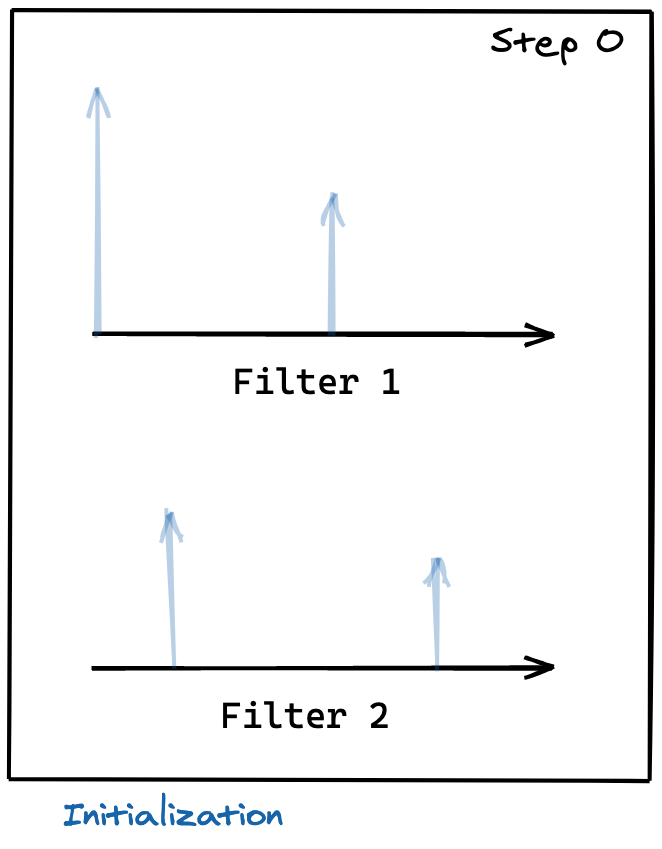
\includegraphics[width=0.5\linewidth]{blaster/echo0.png}\\
    $\downarrow$\\
    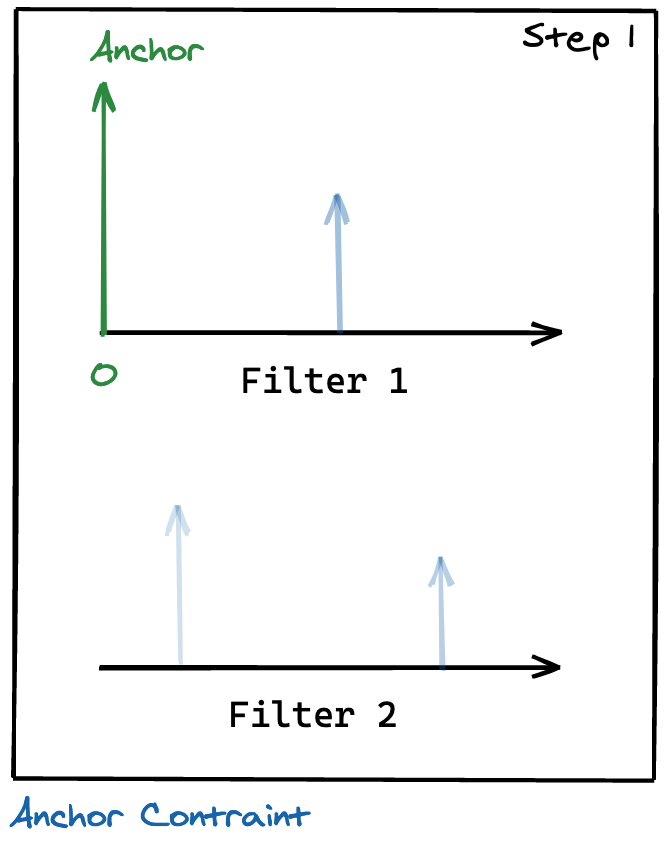
\includegraphics[width=0.5\linewidth]{blaster/echo1.png}\\
    $\downarrow$\\
    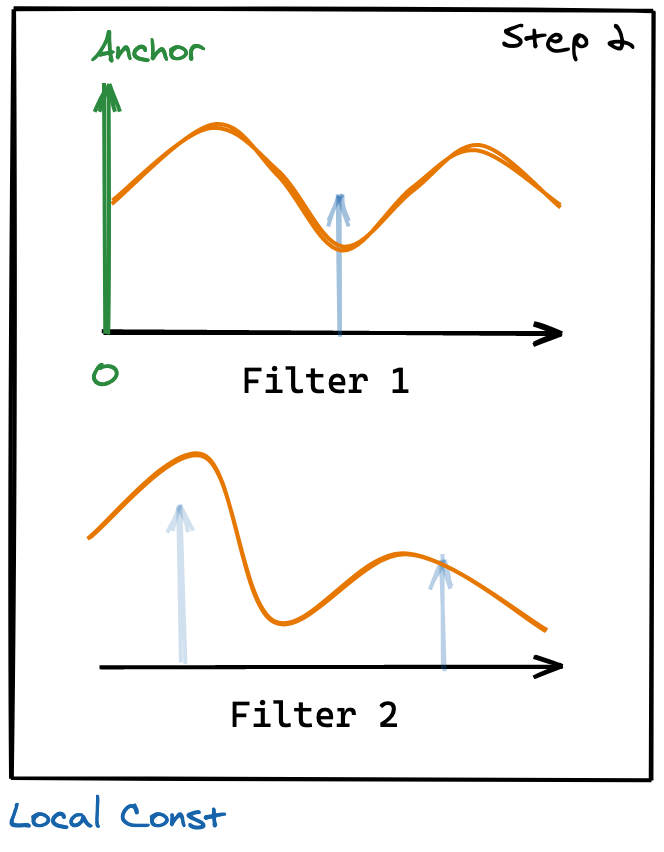
\includegraphics[width=0.5\linewidth]{blaster/echo2.png}\\
    $\downarrow$\\
    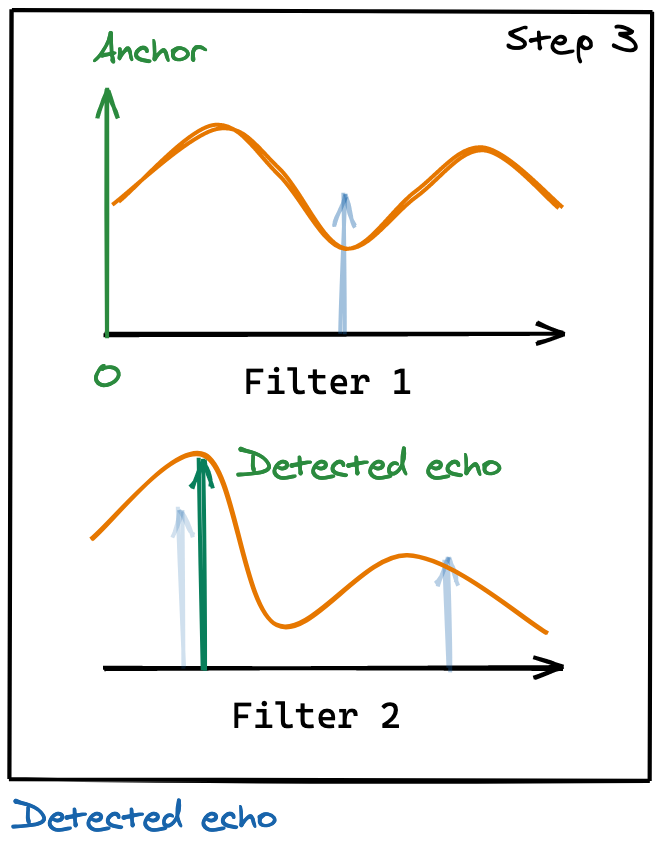
\includegraphics[width=0.5\linewidth]{blaster/echo3.png}\\
    $\downarrow$\\
    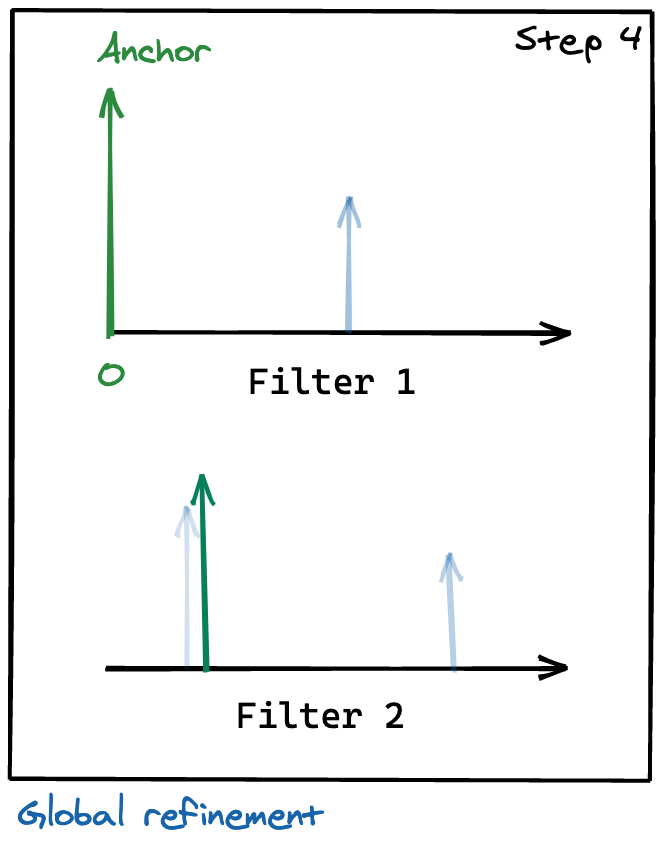
\includegraphics[width=0.5\linewidth]{blaster/echo4.png}\\
    $\downarrow$\\
    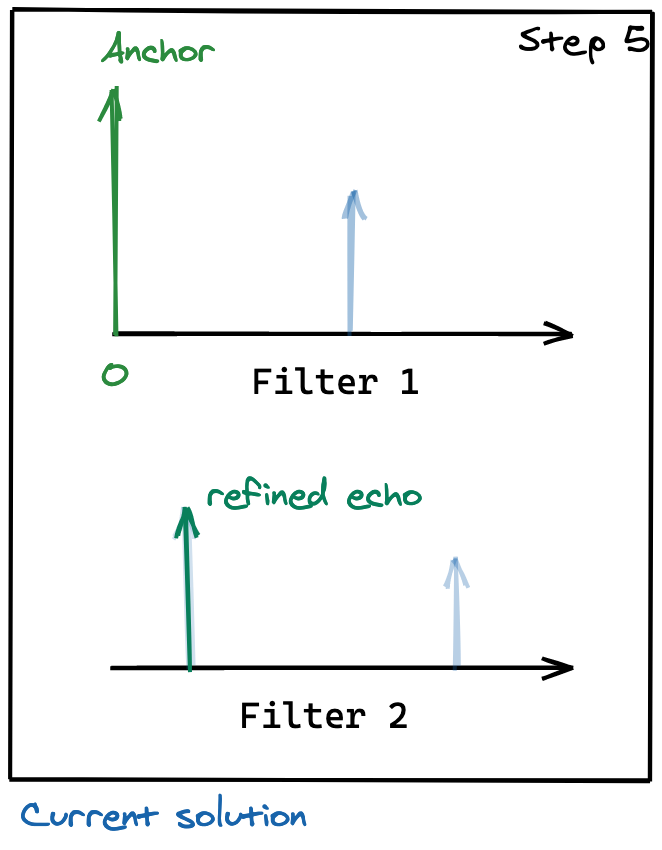
\includegraphics[width=0.5\linewidth]{blaster/echo5.png}
    \captionof{figure}{
        Illustration of the sliding Frank-Wolfe algorithm proposed in~\citeonly{denoyelle2019sliding} in \BLASTER/.
    }
    \label{fig:blaster:sfw}

}

\subsection{The resulting algorithm}
The algorithm used to solve~\cref{eq:blaster:TV-BLASSO} is an of instance the sliding Frank-Wolfe algorithm proposed in~\citeonly{denoyelle2019sliding} to solve~\cref{eq:blaster:TV-BLASSO}.
Detailed descriptions of the steps of the algorithm are given in~\citeonly[Supplementary Material]{di2020blaster}.
In a nutshell, the algorithm iterates over the following steps until a condition on the cost function is met.
\begin{enumerate}
    \item \textit{Anchor constraint}.
    At first the anchor constraint in added arbitrarily on one of the two filters. This is used to initialize the two filters.
    \item \textit{\textit{Local} cost based on Cross-relation}.
    For both the filters, a local cost-function derived from the cross-relation for both the filters is computed.
    At this step either the initialization or a previously found solution is used.
    \item \textit{Find the maximizer}.
    A new candidate echo's location is found as maximizer among the two local cost functions of the previous step.
    \item \textit{Update the amplitudes}.
    By solving a non-negative \LASSO/ problem, all the echo's amplitude coefficients estimated until this point are updated.
    \item \textit{Joint refinement}.
    The position and the coefficient of the current solution are jointly refined to ease numeric resolution using the original cost function.
    \item \textit{Current solution and repeat}.
    The algorithm stops as soon as an iterate satisfies the first order optimality condition associated to the convex problem.
    Otherwise, the algorithm iterates from step 2. using the current solution as input.
\end{enumerate}
These steps are illustrated in~\cref{fig:blaster:sfw}.
% \begin{figure}[h]
%     \begin{fullwidth}
%     \centering
%     \subfloat[echo0][Anchor]{
%         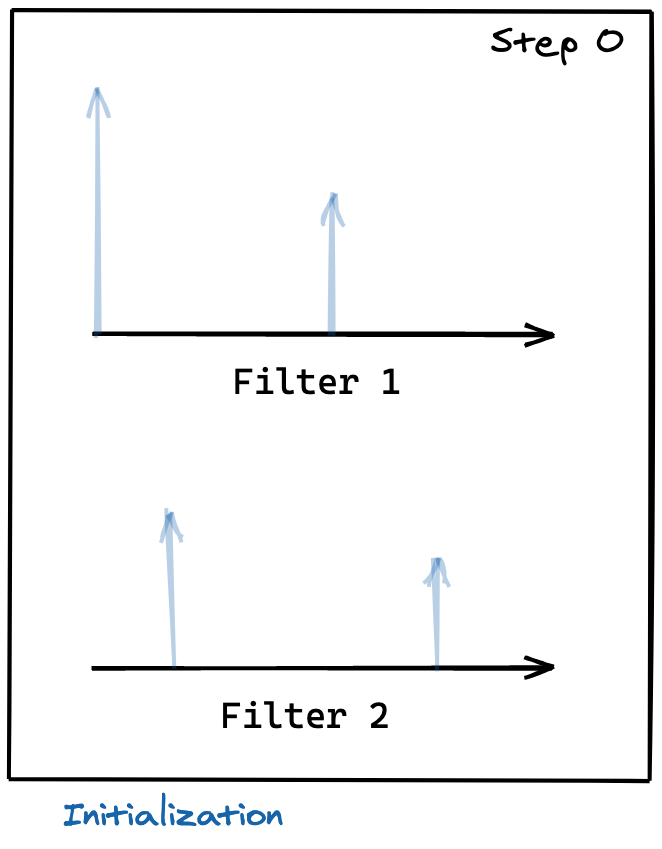
\includegraphics[width=0.13\linewidth]{blaster/echo0.png}
%         \label{fig:blaster:echo0}}
%     \hfill
%     \subfloat[echo1][Local evaluation]{
%         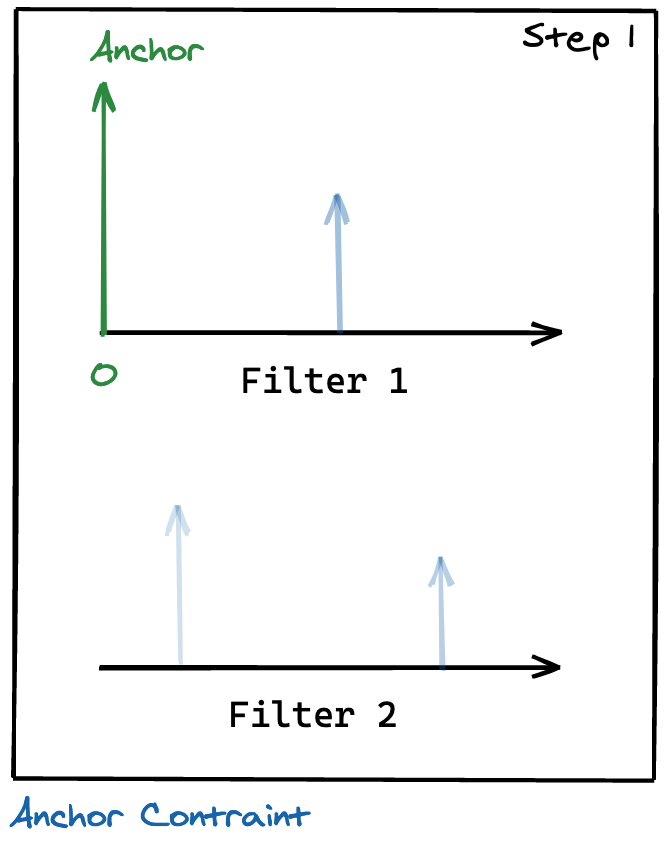
\includegraphics[width=0.13\linewidth]{blaster/echo1.png}
%         \label{fig:blaster:echo1}}
%     \hfill
%     \subfloat[echo2][Maximizer]{
%         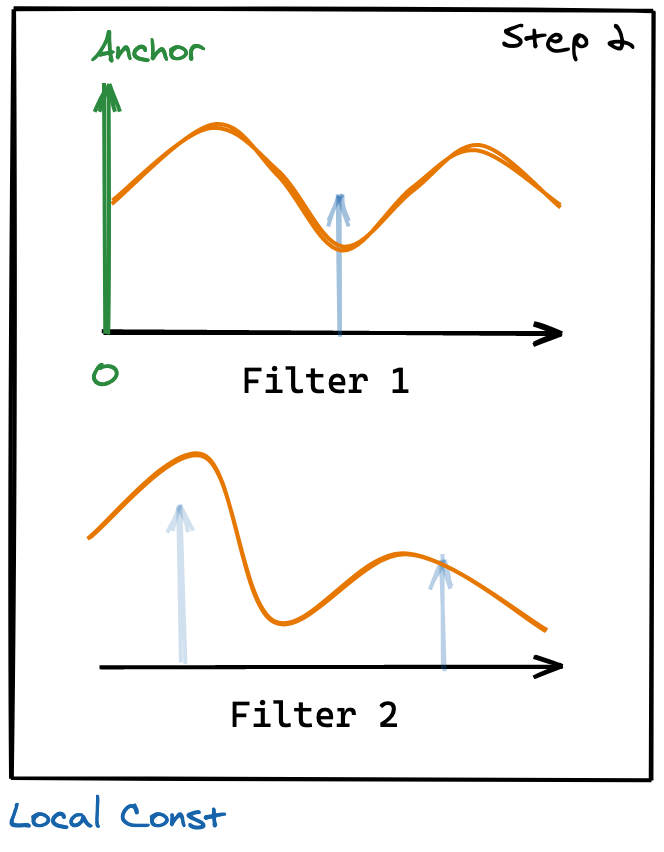
\includegraphics[width=0.13\linewidth]{blaster/echo2.png}
%         \label{fig:blaster:echo2}}
%     \\
%     \subfloat[echo3][Update echoes' amplitudes]{
%         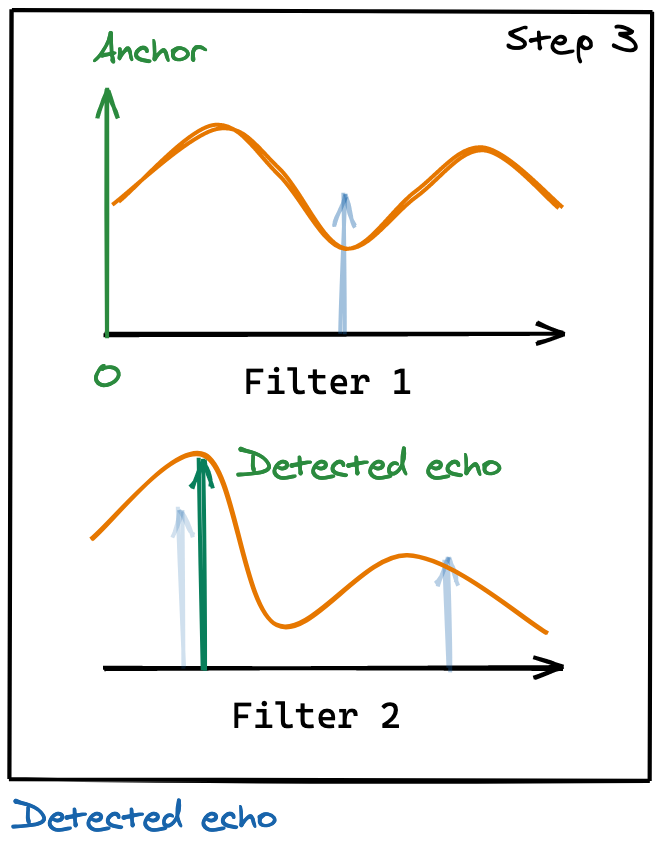
\includegraphics[width=0.13\linewidth]{blaster/echo3.png}
%         \label{fig:blaster:echo3}}
%     \hfill
%     \subfloat[echo4][Joint refinement]{
%         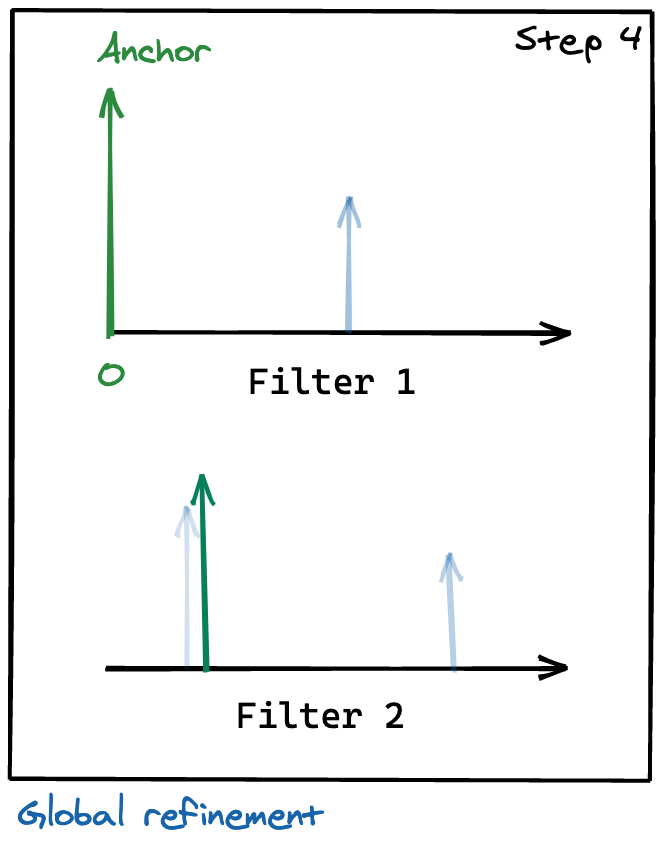
\includegraphics[width=0.13\linewidth]{blaster/echo4.png}
%         \label{fig:blaster:echo4}}
%     \hfill
%     \subfloat[echo5][Current solution]{
%         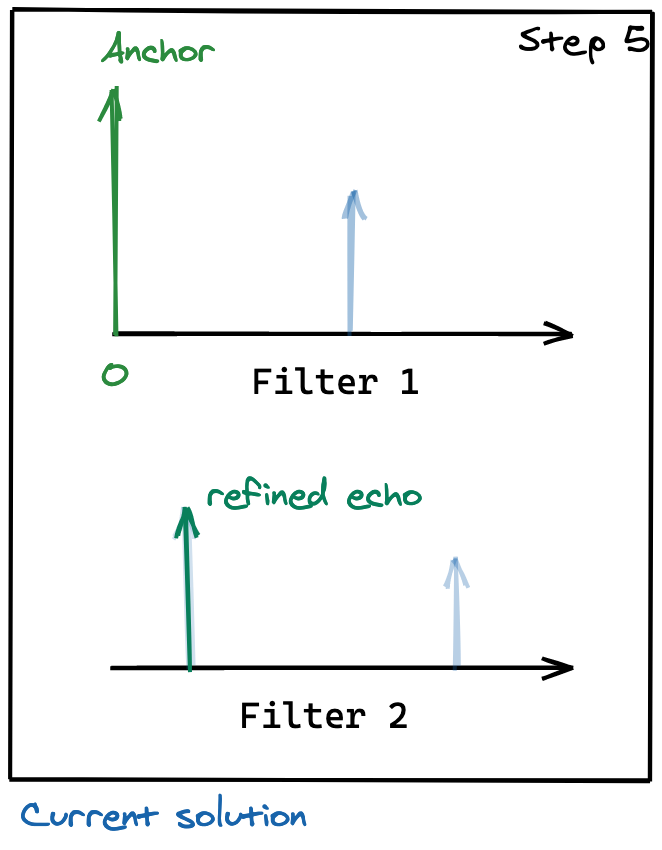
\includegraphics[width=0.13\linewidth]{blaster/echo5.png}
%         \label{fig:blaster:echo5}}
%     \hfill
%     \end{fullwidth}
% \end{figure}

\subsection{Homotopic path for $\lambda$ estimation}\label{sec:blaster:lambda}
Existing works, as well as the proposed one, rely on of the regularization parameter $\lambda$ to weight the sparsity penalty.
However, this becomes an hyperparameter that needs to be carefully tuned according to the input data.
Instead, we propose to compute a \textit{path of solutions} to automatically estimate it in~\cref{eq:blaster:TV-BLASSO}.
In the context of sparse optimization this technique is also referred to as \textit{homotopic path}.
More precisely, let $\lambda_{\max}$ be the smallest value of $\lambda$ such that the null measure is the solution to~\cref{eq:blaster:TV-BLASSO}.
It can be shown that $\lambda_{\max}$ is upper bounded by $\max_{\theta\in\Theta} \kvbar{y^\intercal\opObs\delta_\theta}$.
Starting from $z=1$ and the empty filter, we consider a sequential implementation where the solution of~\cref{eq:blaster:TV-BLASSO} is computed for $\lambda^{(z)}= 10^{-0.05z}\lambda_{\max}$ until the desired number of spikes is found in each channel when incrementing $z$.
For each $\lambda^{(z)}$, we search for a solution of~\cref{eq:blaster:TV-BLASSO} with the solution obtained for $\lambda^{(z-1)}$ as a warm start.

\section{Experiments}\label{sec:blaster:exp}
The proposed method (\BLASTER/) is compared against the non-negative $\ell_1$-norm method (\algoBsn) of~\citeonly{lin2007blind} and the iterative $\ell_1$-norm approach (\algoCrocco) described in~\citeonly{crocco2016estimation}.\sidenote{
    Reference implementations for \algoCrocco{} and \algoBsn{} were kindly provided by the authors of~\citeonly{crocco2016estimation}.
}
The problem is formulated as estimating the time locations of the first $\numEchs=7$ strongest components of the RIRs for 2 microphones listening to a single sound source in a shoebox room. It corresponds to the challenging task of estimating first-order early reflections.
The robustness of the methods is tested against different levels of noise (SNR) and reverberation time (\RT{}).

\mynewline
The quality of AER estimation is assessed in terms of precision\sidenote{
    Since only $K$ time locations are considered in both the ground truth and the estimation, precision and recall are equal.}
in percentage as in the literature of onset detection~\citeonly{bock2012evaluating} and the \RMSEtxt/ in samples.
Both metrics evaluate only the \textit{matched} peaks, where a \textit{match} is defined as being within a small window $\thr$ of a reference delay.
These two metrics are similar to the ones used in~\citeonly{crocco2015room}.

\mynewline
For this purpose we created three synthetic datasets of $1000$ observations each, which are summarized in~\cref{tab:blaster:datasets}.
\begin{table}[ht]
    \begin{sidecaption}[]{
        Summary of the dataset used for evaluation. \epsdice[black]{3} and \epsdice{5} stands for randomly sampled from a continuous and discrete set of values, respectively, with uniform law.
    }[tab:blaster:datasets]
    \centering
    \small
    \begin{tabular}[t]{lccc}
    \toprule
    Dataset      & Signals & SNR [dB] &  $\RT{}$ [s]\\
    \midrule
    \dsetValid     & broadband noise & \epsdice[black]{3} & \epsdice[black]{3}\\
    \dsetSNR       & broadband noise, speech  &\epsdice{5} & $400$ ms\\
    \dsetRT        & broadband noise, speech  &$20$ dB  & \epsdice{5}\\
    \bottomrule
\end{tabular}
    \end{sidecaption}
\end{table}
\\\dsetValid{} is used for tuning the hyperparameter $\lambda$ and the peak-picking parameters for \algoCrocco{} and \algoBsn{} using \RT{} and SNR randomly drawn from $\mathcal{U}[0, 1]$ (sec) and $\mathcal{U}[0, 20]$ (dB) respectively; \dsetSNR{} features SNR value uniformly sampled in $[0, 6, 14, 20, \infty]$ while the \RT{} is kept fixed to $400$ ms; akin the \dsetRT{} is built sampling \RT{} value uniformly in $[200, 400, 600, 800, 1000]$ ms keeping SNR to 20 dB.
Moreover, while for \dsetValid{} broadband signals (white noise) are used as the source, for \dsetSNR{} and \dsetRT{} speech utterances from the TIMIT dataset~\citeonly{garofolo1993timit} are also included.
The signal duration is kept fixed to 1 s with sampling frequency $\Fs = 16$ kHz.
For a given \RT{} value and room with random dimensions, a unique absorption coefficient is assigned to all surfaces based on Sabine's formula (\cref{eq:processing:sabine}).
Then, the two microphones and the source are randomly positioned inside the room.
The parameters of the audio scene are then passed as input to the \pyroomacoustics{} simulator~\citeonly{scheibler2018pyroomacoustics}, which returns the corresponding \acp{RIR} as well as the \textit{off-grid} echo delays and attenuation coefficients computed with the \ISMdef/~\citeonly{allen1979image}.
Note that when generating the data, no samples have been pruned to match any minimal separation condition.
To generate the microphone signals, an over-sampled version of the source signal is convolved with ideal \acp{RIR} at high frequency ($\Fs=1024$ kHz) made up of on-grid Dirac\textit{s}.
The results are later resampled to meet the original $\Fs$ and Gaussian white noise is added to meet the given SNR value.

\mynewline
Finally, as described throughout~\cref{ch:estimation}, \algoCrocco{} and \algoBsn{} uses tuned peak picking step to identity the echoes.
Here the same peak picking technique provided with reference implementation of these methods was used and tuned on a small validation set.


\newthought{Quantitative results} are reported in ~\cref{fig:error_precision_snr_rt}, ~\cref{fig:error_precision_kecho} and ~\cref{tab:error_precision_thr}.
Here, for both RMSE and precision and for both broadband and speech signal, the metrics are displayed against the dataset parameters.
We observe that \algoBsn{} performs worst in all tested conditions, possibly due to its strong reliance on the peak picking step.
For $\numEchs=7$ or higher, \algoBraire{} yields similar or slightly worse performance than \algoCrocco{} for the considered noise and reverberation levels, with decreasing performance for both as these levels increase.
Using speech rather than broadband signals also yields worse results for all methods.
However, the echo timing RMSE is significantly smaller using \algoBraire{} due to its off-grid advantage.
We also note that \algoBraire{} significantly outperforms \algoCrocco{} on the task of recovering $\numEchs=2$ echoes.
As showed in Tab.~\ref{tab:error_precision_thr}, in mild conditions ($\RT = 200$~ms, $\mathtt{SNR} = 20$~dB), up to 68\% of echoes can be retrieved by \algoBraire{} with errors lower than a quarter of sample in that case.
This is promising since the practical advantage of knowing the timings of two echoes per channel has been demonstrated in~\citeonly{di2019mirage} (See~\cref{ch:mirage}), and in~\citeonly{scheibler2018separake} (See~\cref{ch:separake}).

\begin{figure}[ht]
    \centering
    \begin{fullwidth}
        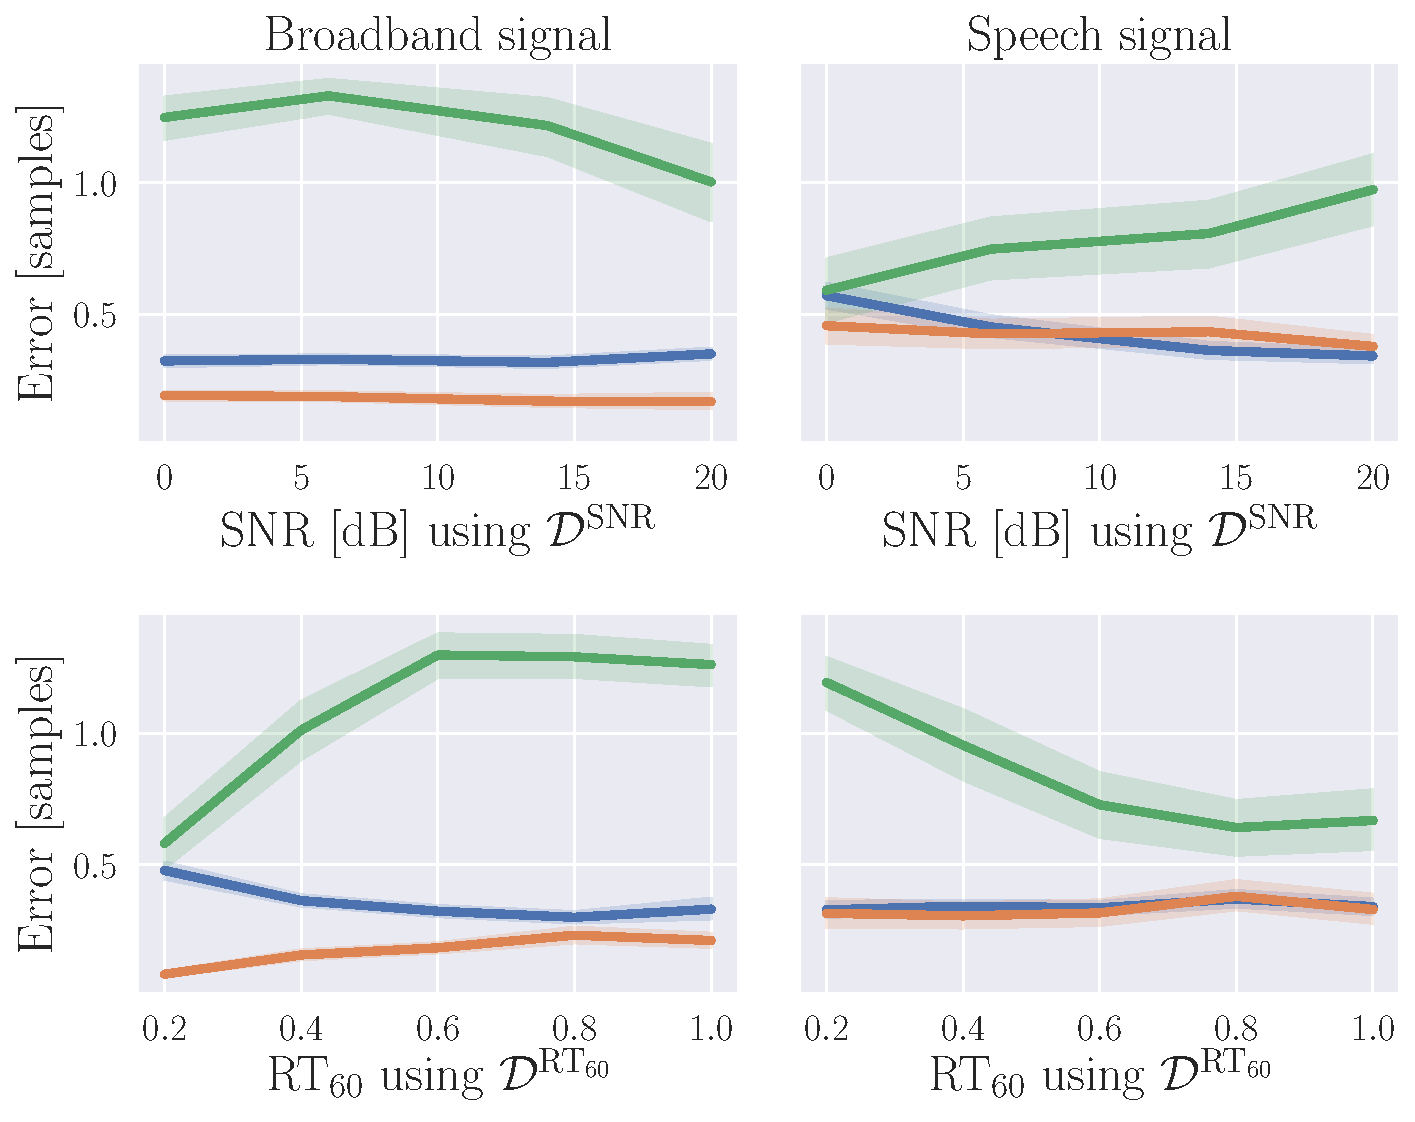
\includegraphics[width=.49\textwidth]{figures/blaster/e_k-7_thr-2_bns_crocco_blaster.pdf}
        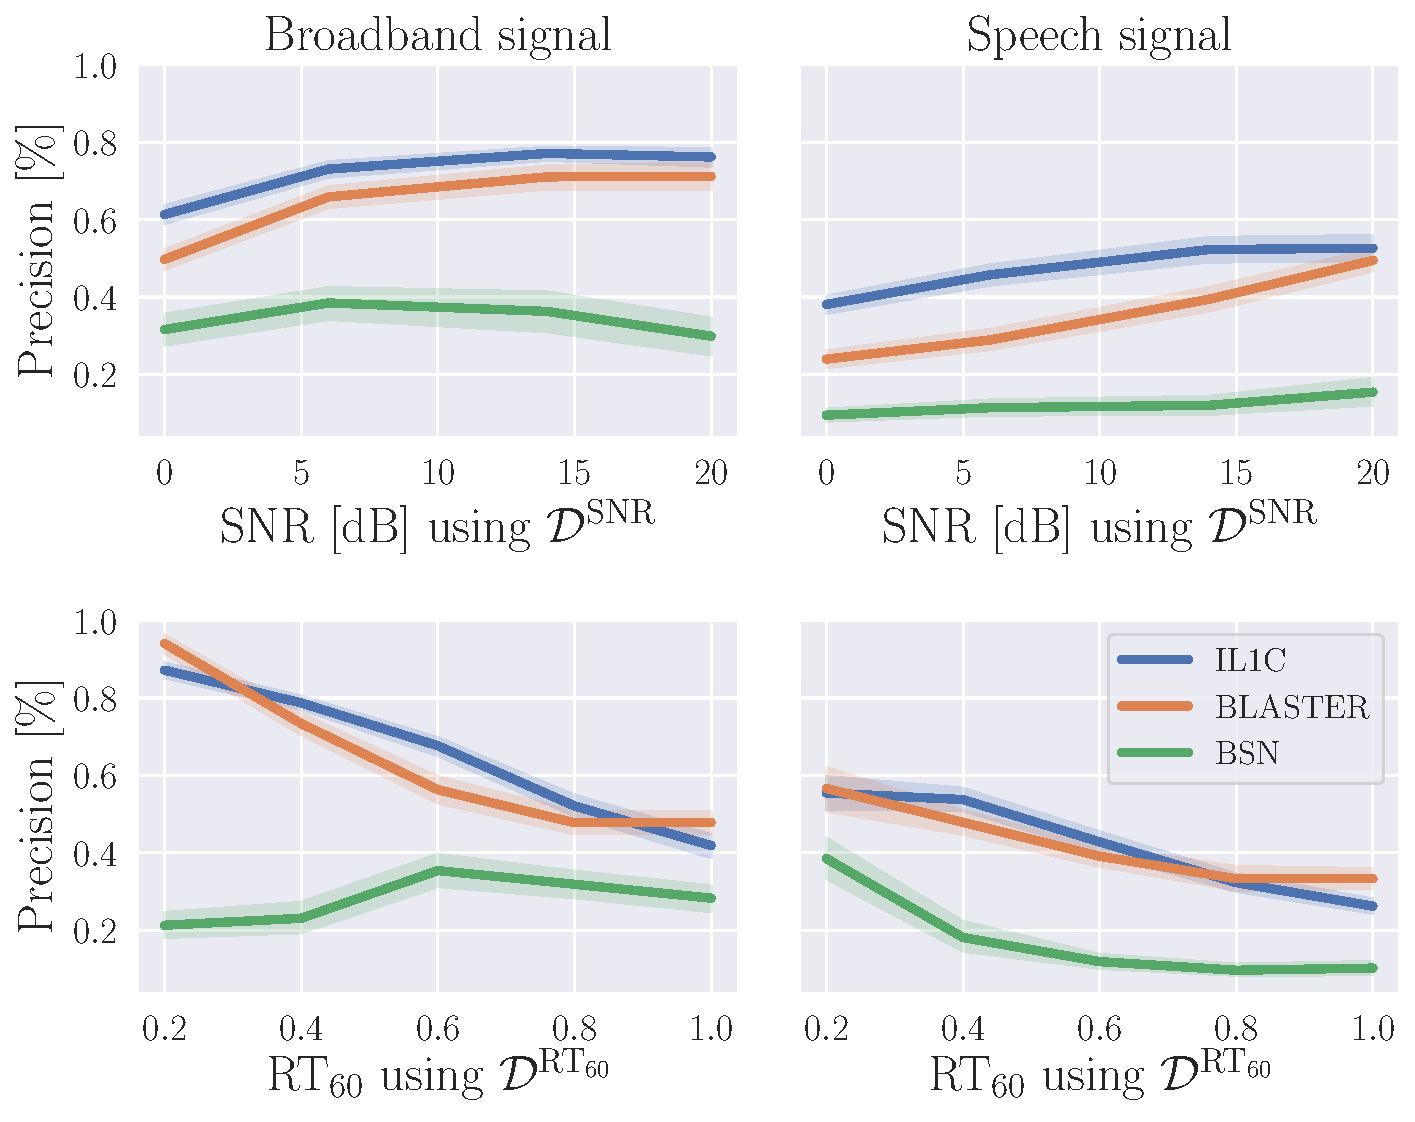
\includegraphics[width=.49\textwidth]{figures/blaster/p_k-7_thr-2_bns_crocco_blaster.pdf}
        \caption{%
            \label{fig:error_precision_snr_rt}
            Mean error (left) and precision (right) versus SNR level (top) and \RT{} level (bottom) using broadband and speech signals for the task of recovering $\numEchs=7$ echoes. A threshold of $\tau_{\textrm{max}}=2$ samples is used to compute the precision.
            Error bands denotes 95\% confidence intervals.
        }

    \end{fullwidth}
\end{figure}

\begin{table}[ht]
    \begin{sidecaption}[]{
        Precision for different threshold $\thr$ in samples for the recovery of $R = 2$ and $7$ echoes, $\RT = 200$~ms and $\SNR = 20$~dB.
    }[tab:error_precision_thr]
    \centering
    \footnotesize
    %\begin{table}[t]
    {
        \centering
        \begin{tabular}{lccccc|ccccc}
        \toprule
               & \multicolumn{10}{c}{Precision [\%]}	\\
               \cline{2-11}
               & \multicolumn{5}{c|}{R = 2 echoes} & \multicolumn{5}{c}{R = 7 echoes} \\
               %
               \hline
               %
    $\thr$ & $0.5$ & $1$ & $2$ & $3$ & $10$ & $0.5$ & $1$ & $2$ & $3$ & $10$ \\ \hline
    BSN &  8 &           9 &          27 &          46 &           62 &           5 &           8 &          38 &          54 &  {73}  \\
    IL1C &           51 &          55 &          55 &          56 &           58 &          42 &          53 &          55 &          56 &         58 \\
    BLASTER & \textbf{68}  & \textbf{73}  & \textbf{74}  & \textbf{75}  & \textbf{75}   &{46}  &          53 &  {56}& {57} &         61 \\
    \bottomrule
    \end{tabular}
    }
    %\end{table*}


    % %\begin{table*}[t]
    % {
    %     \centering
    %     \scriptsize
    %     \begin{tabular}{lcccccccccc|ccccc|ccccc}
    %     \toprule
    %            & \multicolumn{10}{c|}{Error [samples]}                                                                                               & \multicolumn{10}{c}{Precision [\%]}                                                                           \\ \cline{2-21}
    %            & \multicolumn{5}{c|}{K = 2 echoes}                                           & \multicolumn{5}{c|}{K = 7 echoes}                     & \multicolumn{5}{c|}{K = 2 echoes}                     & \multicolumn{5}{c}{K = 7 echoes}                     \\ \hline
    % $\thr$ & $0.5$ & $1$ & $2$ & $3$ & \multicolumn{1}{c|}{$10$} & $0.5$ & $1$ & $2$ & $3$ & $10$ & $0.5$ & $1$ & $2$ & $3$ & $10$ & $0.5$ & $1$ & $2$ & $3$ & $10$ \\ \hline
    % \algoBsn &  \textbf{0.01} &\textbf{0.05}&        1.07 &        1.53 &\multicolumn{1}{c|}{2.85}         &\textbf{0.05}&        0.24 &        1.19 &        1.53 &         3.09 &           8 &           9 &          27 &          46 &           62 &           5 &           8 &          38 &          54 & \textbf{73}  \\
    % \algoCrocco &        0.20 &        0.23 &        0.24 &        0.26 &\multicolumn{1}{c|}{0.40}         &        0.20 &        0.28 &        0.33 &\textbf{0.37}&\textbf{0.83} &          51 &          55 &          55 &          56 &           58 &          42 &          53 &          55 &          56 &         58 \\
    % \algoBraire &        0.06 &        0.10 &\textbf{0.14}&\textbf{0.20}&\multicolumn{1}{c|}{\textbf{0.34}}&        0.13 &\textbf{0.20}&\textbf{0.32}&        0.42 &         1.48 &\textbf{68}  &\textbf{73}  &\textbf{74}  &\textbf{75}  &\textbf{75}   &\textbf{46}  &          53 &  \textbf{56}& \textbf{57} &         61 \\
    % \bottomrule
    % \end{tabular}
    % }
    %\end{table}
    \end{sidecaption}
\end{table}

\begin{figure}[t!]
    \begin{sidecaption}[]{
        Precision versus number of echoes $R$ to be retrieved for broadband (left) and speech (right) signals with \RT{} = $400$ ms and SNR = 20 dB.
        Error bands denotes 95\% confidence intervals.
    }[fig:error_precision_kecho]
    \centering
    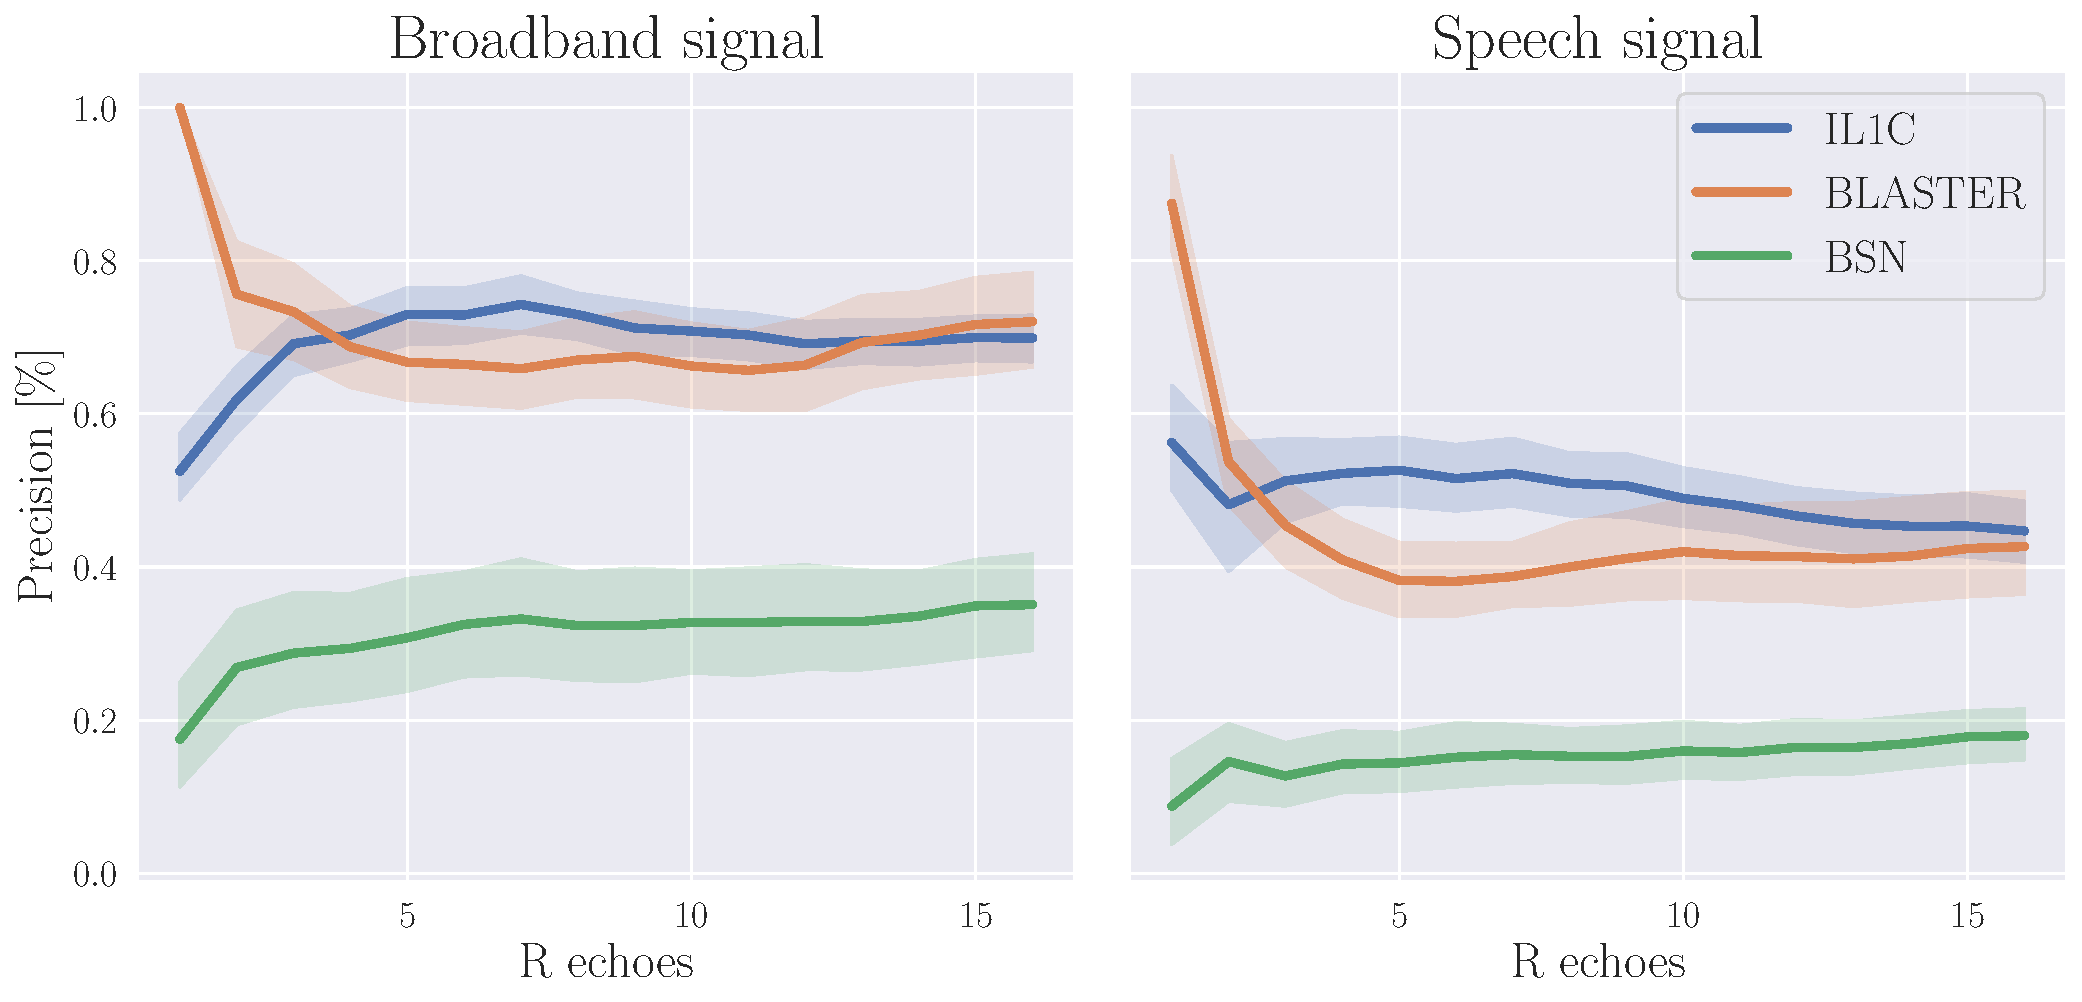
\includegraphics[width=\linewidth]{figures/blaster/p_k-7_thr-2_bns_crocco_blaster-peak_withRechoes.pdf}
    \end{sidecaption}
\end{figure}

\section{Conclusion}
In this chapter we presented a novel knowledge-driven blind, off-grid echo retrieval method, based on the framework of continuous dictionaries.
The particular ``knowledge'' we used is the echo model for the early part of the \acp{RIR}.
The main motivation behind this approach is to overcome the pathological limitation of classical methods for \ac{BCE}, discussed in the previous chapter.
Despite an heavy mathematical formulation, it can seen as as the continuous extension of a \LASSO/ problem used for addressing \ac{BCE}.
Comparisons with state-of-the-art approaches on various noise and reverberation conditions show that this method performs best when the number of echoes to retrieve is small.
Future works will include many exciting directions, such as:
\begin{itemize}
    \item extending the framework to multichannel recordings using the Multichannel cross-relation, as already envisioned by the related works~\citeonly{crocco2015room,lin2008blind};
    \item compare this approach with other off-grid \AER/ methods  ~\citeonly[Chapter 6]{peic2020sparse};
    \item adapt this approach to deal with \ReTF/ which allow for source-independent acoustic features (See~\cref{ch:dechorateapp});
    \item use deep learning approaches to estimate the level of sparsity (\aka/ number of the most relevant echoes) in the \acp{RIR};
    \item validate the approach on real-world recordings, such as the one provided by the \ac{DECHORATE} dataset (See~\cref{ch:dechorate}).\qed
\end{itemize}
% \chapter{\library{Lantern}: Data-driven Acoustic Echo Retrieval}\label{ch:lantern}

\marginpar{%
    \footnotesize
    \textbf{Keywords:} Acoustic Echo Retrieval, TDOA Estimation, Supervised Learning, Deep Learning, Robust Regression.
    \\\textbf{Resources:}
    \begin{itemize}
        \item \href{https://ieeexplore.ieee.org/document/8683534}{ICASSP2018 Paper}
        \item \href{https://github.com/Chutlhu/MIRAGE}{Code}
        \item \href{https://sigport.org/documents/mirage-2d-sound-source-localization-using-microphone-pair-augmentation-echoes}{ICASSP2018 Poster}
    \end{itemize}
}
\newthought{Synopsis} \synopsisChLantern

\mynewline
This chapter is structured in two sections: one devotes to present a quick overview deep learning model and how to train them, and one discusses their application to echo estimation.
The material concerning the first section are a personal digestion of material available in standard machine learning text book, such as~\citeonly{bishop2006pattern,goodfellow2016deep},
and audio related ones~\citeonly{vincent2018audio,muller2015fundamentals}.
We mention the recent comprehensive work of~\citeonly{purwins2019deep} on deep learning for general audio signal processing.
In the second section present part of the previously published work~\cite{di2019mirage} and of a technical report~\cite{di2019honda}.

\section{Introduction}
Recently \acfp{DNN} have capture the attention of many research field, due to recent advances that allow for faster implementation and training, and considerable performance improvement.
Therefore, \acp{DNN}s have been widely used in many domains.
They belong to the class of \textit{supervised} learning or \textit{data-driven} models, where the training step is performed on labeled data, namely input-output pairs.
The inclusion of these models in audio signal processing tasks has meant a considerable improvement in the performance, in particular audio and music source separation, speech enhancement, source localization (see  the related sections in~\cref{ch:application}).
\\Moreover, respect to traditional machine learning methods, the use of deep learning models presents other advantages.
They are flexible and adaptable across tasks; for instance, \acf{CNN}-based models from Computer Vision can be adapted for audio source separation (\eg/,~\citeonly{xiao2016deep, sainath2017multichannel, perotin2018crnn}), and for source localization(\eg/, ~\citeonly{chakrabarty2017broadband,vesperini2018localizing,nguyen2018autonomous,salvati2018exploiting}).
Furthermore, \acp{DNN}s reduce --- even remove --- the step of designing hand-crafted feature, by including the feature learning as part of the learning process.
\\Other
\marginpar{
    \itshape\footnotesize
    As part of a first investigation in this thesis work, the \acf{GLLiM} framework was considered for echo estimation.
    In fact, this thesis initially as a natural following up of the work~\citeonly{gaultier2017vast}.
    Then, we oriented our attention towards \ac{DNN} models which gave already satisfactory results.
    The highly non-linear nature of the mapping between echoes' properties and acoustic features which collides with the locally-linear assumption behind \ac{GLLiM}.
    Nevertheless, we recognize other benefits of the \ac{GLLiM} framework which cannot be found in \ac{DNN}-based approach.
    For instance, the ability of considering input missing data or including prior statistical information in the model.
} supervised learning methods have been proposed in the literature of audio processing, such as \ac{GMM}-based frameworks~\citeonly{laufer2013relative,deleforge2015acoustic,gaultier2017vast}.
This frameworks allows to build power models based on probabilistic prior knowledge and are compete with \ac{DNN} models in case of small training dataset.
However they ofter require strong assumption of the nature of the mapping between input-output pairs, such as (local-)linearity or independency between the variables.

\mynewline
The use of supervised learning models (not only the \ac{DNN}), presents some disadvantages.
One of the most relevant ones is their dependence on annotated data.
This is important bottleneck in audio signal processing task, because collecting and annotating comprehensive real-wold acoustic data is not trivial, since it requires proper tools, expertise and time.
In order to overcome this issue, a standard approach nowadays is to used training data generated by acoustic simulators.
We will refer to this approach as \textit{virtually supervised learning} and it provides a great versatility, for instance:
\begin{itemize}
    \item many different acoustic condition can be include in the training data,\\\eg/, different \acf{RT$_{60}$} and \acf{SNR} levels;
    \item a precise (up to computer precision) annotation of the data come directly,\\\eg/ spatial, temporal information of the audio scene events;
    \item and finally, the data can be potentially re-used for different application,\\\eg/, localization, separation, diarization, \etc/;
\end{itemize}
Therefore, the simulators provide a direct mapping for the parameters of interest to synthetic observations, which learning-based models aim to invert.
Besides, the solutions obtained in a data-driven fashion suffer from bias depending on the dataset used and may not be able to generalize to real-world scenario.
Interestingly, the work in~\citeonly{nguyen2018autonomous} discusses an automatic approach for collecting, annotating data automatically as a pre-calibration step.
However, this approach is possible only with certain technology (the authors programmed a humanoid robot equipped with a binaural hearing system that build a training set automatically).

\mynewline
The following sections gives a quick overview of relevant models used in our work with the intention of motivating the use for echo estimation.
The review includes basic theory behind neural networks and deep learning, optimization and loss functions, as well as the aspects related to training on
acoustic simulators.

\section{Deep Learning Model}

\subsection{Multi-layer perceptions}\label{subsec:lantern:mlp}
\acf{MLP} are simple and basic modules of \ac{DNN} and are also known as \textit{fully-connected} or \textit{dense layers}.
They consist of a sequence of layer, each of which defined by an affine transformation followed by a non-linearity function:
\begin{equation*}
    \bfy = f(\bfW \bfx + \bfb)
    ,
\end{equation*}
where
\newcommand{\Din}{\ensuremath{D_{\text{in}}}}
\newcommand{\Dout}{\ensuremath{D_{\text{out}}}}
\begin{itemize}
    \item $\bfx\in\bbR^{\Din}$ is the input,
    \item $\bfy\in\bbR^{\Dout}$ is the output,
    \item and $\bfb\in\bbR^{\Dout}$ and $\bfW\in\bbR^{\Dout \times \Din}$ are the \textit{bias vector} and the \textit{weight matrix}, respectively.
\end{itemize}
The function $f(\cdot)$ is a non-linear \textit{activation} function, which allows the model to learn non-linear structures.
Models built with these layers are typically used to map input to a representation space where problems (\eg/, classification and regression) can be addressed more easily.
The main drawback of these simple models is that are not invariant to scaled or shifted input.
Since in audio data, gain, temporal and frequency variations are common, they not suitable.
Nevertheless, \acp{MLP} are used in combination with other type of layers, such as \acfp{CNN}, \acfp{RNN}.

\newthought{Non-linear activation functions} are one of the key feature of \acp{DNN}.
Thanks to these, the model are able to achieve more \textit{expressive power} with respect to linear models~\citeonly{goodfellow2016deep}.
Without these functions, it can be shown that composition of affine transformations, is equivalent to a single affine transformation.
Therefore, the activation functions make the model capable to accounts for more complex relationships between the input and the output than an affine transformation.
Typical examples of these function are, for instance, hyperbolic tangent, the Sigmoid function, and \acf{ReLU}.

\subsection{Convolutional neural networks}\label{subsec:lantern:cnn}
The \ac{CNN} consists in convolutional layers that have been introduced to overcome some limitations of the simple linear ones.
In a nutshell, the consists of learnable kernel functions that are convolved with their input.
Therefore, they are characterized by
\begin{itemize}
    \item shift-invariance property, and can be used to reduce the model complexity since the same kernel can be used at different input location;
    \item the ability to detect local structures at different level of abstraction in the network (see~\cref{fig:lantern:features}).
\end{itemize}
Using a Python-like notation, a 2D-dimensional convolutional layer is defined by the following equation:
\begin{equation*}
    \bfY[:,:,k] = f( \sum_{i=0}^{I-1} \bfW[:,:,i,k] \convDis \bfX[:,:,i] + \bfb[:,:,k])
    ,
\end{equation*}
where
\begin{itemize}
    \item $\bfX_k\in\bbR^{F \times T \times I}$ and $\bfY_c\in\bbR^{A \times B \times K}$ are input and output tensors of dimension, respectively.
    \item $i\in\klist{0,I}$ denotes the channel dimensions;\sidenote{
        In \ac{DNN} community is common refer the input dimensions as channels.
        Based on the application, such channel \textit{do not necessarily} corresponds to the channel of microphone recordings.
    }
    \item $k\in\klist{0,K}$ denotes output;
    \item the tensors $\bfW$ and $\bfb$ denotes the weight and bias tensors, respectively;
    \item $f$ is an activation function;
    \item and, $\convDis$ denotes discrete convolution;
\end{itemize}
\ac{CNN} can be designed for either 1D or 2D convolution, or combination of them.
In general, in audio 1D convolution layer are used to process the time-domain or frequency-domain input, whereas the 2D convolutional layer are used for time-frequency representation, such as spectrograms.
The output of a convolutional layer consist of a collection local convolution operation which are typically referred to as \textit{feature map}.
It is common to use \ac{CNN} architectures combining multiple convolutional layers with \textit{pooling layers} in between.
Pooling layers are used to down-sample the features map.
Beside of reducing the model complexity (\ie/, number of free-parameters), pooling layer subsequently reduce the size of the data as the model goes ``deeper''.
In this way deeper layers can integrate larger extents of the data and extract spatial (in the sense of the input dimensions) features at higher scale.
The typical pooling operator are the \textit{max-pooling} and \text{mean-pooling} which samples non-overlapping patches by keeping the biggest and the average value in the region, respectively.

\subsection{Hybrid architectures}
As mentioned earlier, modern \ac{DNN} architectures consist of combination of different type of layers.
For instance, \acp{CNN} are used to overcome the lack of shift and scale invariance the \ac{MLP} suffers and allows to extract spatial features.
In contrast, \acp{MLP} offers a simple mapping from big-dimensional space to smaller ones, suitable for classification and regression problems.
Therefore hybrid architecture are now the standard for deep learning models.

\subsection{Learning and optimization}
\newcommand{\params}{\ensuremath{\boldsymbol{\theta}}}
Per se, the \ac{DNN} models consists of thousands of parameters $\params$.
In order to learn to preform a specific task, such as regression or classification, they need to be optimized.
To optimize the parameters $\params$, a variants of gradient descent algorithm is usually implemented.
A \textit{loss function} $\calL_{\params}(\hat{\bfY},\bfY)$ measure the difference between the predicted values $\hat{\bfY}$ and the desired on $\bfY$.
The optimization processes then iteratively update the parameters $\params$ so the loss function is minimized, that is
\begin{equation*}
    \params \gets \params - \eta \knabla_{\params} \calL_{\params}(\hat{\bfY},\bfY)
    ,
\end{equation*}
where $\eta$ is referred to as \textit{learning rate} and accounts for how much to update the $\params$ at each iteration.
Due to the compositive structure of the \ac{DNN}, the gradient $\knabla_{\params} \calL_{\params}(\hat{\bfY},\bfY)$ is compute via the chain rule, using the \textit{back propagation} algorithm.
\\The \textit{Stochastic Gradient Descent} is a variant of the gradient descent algorithm which has become the standard for training \acp{DNN} today.
It was introduced to solve computational and memory load issues due to large training since it approximate the gradient at each step on a mini-bach of data samples.
\\Another common practice in the optimization of \acp{DNN} is to use \textit{early stopping} criteria.
This allows to stop the training upon some condition on the loss function, for instance, when it is not improving after certain amount of iterations.
Finally, the early stopping can be computed on different metric then the one used for optimizing the network's parameters.
As the loss function requires to be differentiable, some metrics cannot be directly optimized, but their performances can be determined a posteriori on a \textit{validation set} and used to avoid overfitting.

\section{Learning-based Acoustic Echo Retrieval}
As a first step, we will use \ac{DNN} to estimate the timings of the first and strongest echo from stereophonic recordings, \ie/ $\numEchs=1$.
In order to disambiguate this reflection from the other, we consider a simplified scenario: close-surface scenario, shown in~\cref{fig:lantern:scene}.
\marginpar{%
    \centering
    \footnotesize
    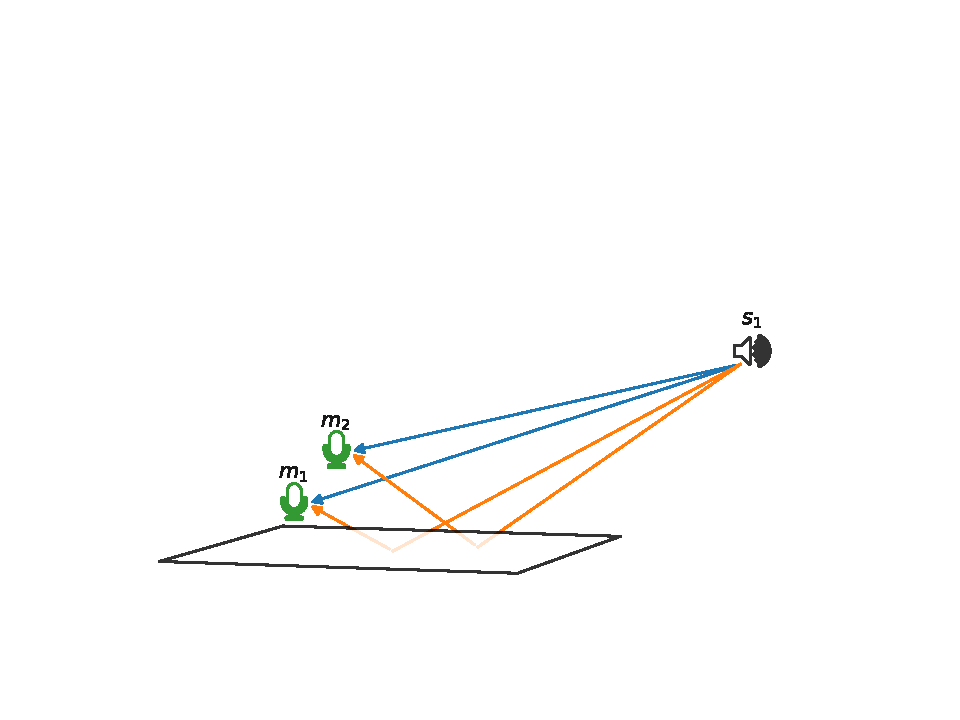
\includegraphics[trim={50 70 50 150},clip,width=\linewidth]{mirage/scene.pdf}
    \captionof{figure}{%
        Typical setup with one source source recorded by two microphones.
        The illustration shows direct sound path (blue lines) and resulting first-order echoes (orange lines).}
    \label{fig:lantern:scene}
}.
This is motivated by the application to \acf{SSL} that will be discussed in~\cref{ch:mirage}.
The reason why we consider only microphone-pair is that this approach can be generalize later to microphone array.
In fact, by considering all the pairs, it is possible to aggregate all their estimation in a second step using the knowledge about the array geometry.
Such an approach can be referred to the \ac{SRP-PHAT}~\citeonly{dibiase2001robust} algorithm used is \ac{SSL}.
In the remaining part of this chapter, we will discuss how to achieve robust first-echo estimation and how it could be generalized to multiple echoes.

\subsection{Simple Case: $\numEchs = 1$}
Our approach is to train a \ac{DNN} on a dataset simulating the considered close-surface scenario.
Under this assumption and the \acf{STFT} signal model presented in~\cref{eq:processing:stft}, we can consider the following simplified model for the \acfp{RTF},
\begin{equation}\label{eq:mirage:rir}
    \FLT_\idxMic[k] = \sum_{\idxEch=0}^{\numEchs=1}  \; \alpha_\idxMic^{(\idxEch)}[k] \; \cste^{- \csti 2 \pi f_k \tau_\idxMic^{(\idxEch)}} \; + \; \varepsilon_\idxMic[k],
\end{equation}
where $\tau_\idxMic^{(\idxEch)}$ and $\alpha_\idxMic^{(\idxEch)}[k]$ are the echoes's time of arrival and amplitude, respectively.
The $f_k$ denotes $k$-th frequency bin and the error term $\varepsilon_i[k]$ collects later echoes, the reverberation tail, diffusion, and noise.

\mynewline
We model the \AER/ problem as multi-target regression problem, namely the output on the model are multiple real-valued parameters.
Following the approaches suggested in~\citeonly{deleforge2015acoustic,gaultier2017vast}, we consider the instantaneous \acf{ILD} and the \ac{IPD} (see~\cref{eq:mirage:features} as input features.
As discussed in~\cref{subsec:processing:steering}, the \ac{ILD} and \ac{IPD} can be estimated from the \STFT/ of the microphone signals, such as,
\begin{equation} \label{eq:mirage:features}
\begin{cases}
    \ild[k]  =& \tfrac{1}{T} \sum_{l=1}^T \log{\abs{\frac{\MIC_2[k,l]}{\MIC_1[k,l]}}}, \\
    \ipd[k]  =& \tfrac{1}{T} \sum_{l=1}^T \frac{\MIC_2k,l]/ \abs{\MIC_2[k,l]}}{ \MIC_2k,l] / \abs{\MIC_1[k,l]}},\\
\end{cases}
\end{equation}
where $\MIC_i[k,l]$ is the \ac{STFT} of the $i$-th microphone.
\\More precisely, the input of the network is
\begin{equation*}
    \xi = \klist{ \ild, \kRe\set{\ipd}, \kIm\set{\ipd}}
    ,
\end{equation*}
namely the concatenation of the above features for all the frequencies.
Here $\kRe\set{\cdot}$ and $\kIm\set{\cdot}$ denote real and imaginary part operators, respectively.
Note that for the \ac{IPD}, the frequency $k=0$ is discarded because it is constant for every observation.

\mynewline
Initial investigation shown that learning directly the echoes arrival time and their amplitude yield huge estimation error, probable to the complexity of the task.
Motivated by the application in \ac{SSL} discussed in~\cref{ch:mirage}, we consider only the \acfp{TDOA} between the direct path propagation.
\begin{align}
    \tau_\mathtt{TDOA}  &= \tfrac{1}{c} \norm{\positionMicrophone_2 - \positionSource} - \tfrac{1}{c} \norm{\positionMicrophone_1 - \positionSource} = \tau_2^{(0)} - \tau_1^{(0)} \quad[\text{s}],\\
    \tau_\mathtt{iTDOA} &= \tfrac{1}{c} \norm{\mathring{\positionMicrophone}_2 - \positionSource} - \tfrac{1}{c} \norm{\mathring{\positionMicrophone}_1 - \positionSource} = \tau_2^{(1)} - \tau_1^{(1)} \quad[\text{s}],\\
    \tau_{\mathtt{TDOE},1}  &= \tfrac{1}{c} \norm{\mathring{\positionMicrophone}_1 - \positionSource} - \tfrac{1}{c} \norm{\positionMicrophone_1 - \positionSource} = \tau_1^{(1)} - \tau_1^{(0)} \quad[\text{s}],
\end{align}
where $\mathring{\positionMicrophone}_i$ denotes the position of the image of the microphone at position $\positionMicrophone_i$ with respect to the reflector.
Note that $\tau_{\mathtt{TDOE},2} = \tau_\mathtt{iTDOA} + \tau_{\mathtt{TDOE}, 1} - \tau_\mathtt{TDOA}$.
These three quantities are directly connected to \RIRs/, as illustrated in~\cref{fig:lantern:rirs_tdoa}\marginpar{%
\centering
\footnotesize
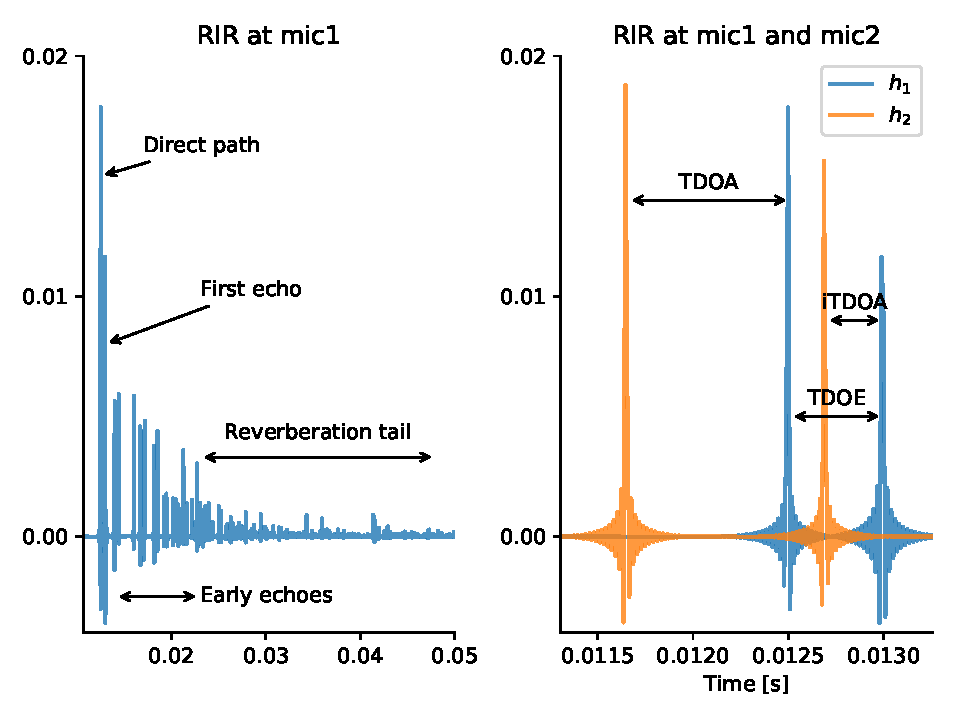
\includegraphics[trim={82mm 0 0 0},clip,width=\linewidth,height=7cm]{mirage/rirs.pdf}
\captionof{figure}{%
    Superposition of two \acp{RIR} and visualization of time difference of arrival between direct paths (\ac{TDOA}), first echoes (\ac{iTDOA}) and direct path and first echo (\ac{TDOE}).}
\label{fig:lantern:rirs_tdoa}
}. Let $V = \klist{\tau_{\mathtt{TDOA}}, \tau_{\mathtt{iTDOA}}, \tau_{\mathtt{TDOE},1}}\in\mathbb{R}^3$ be the vector of the parameters of interest
and $\calV = \set{\mathtt{TDOA}, \mathtt{iTDOA}, \mathtt{TDOE}_1}$ the set of corresponding labels.

\mynewline
In general, the mapping between $V$ and the proposed feature is not unique.
In particular, this happen when $\tau_2^{(\idxEch)} = \tau_1^{(\idxEch)}$ for $\idxEch=\set{0,1}$.
In order to avoid this, we preventively pruned all the entries with $| \tau_2^{(\idxEch)} - \tau_1^{(\idxEch)} | < 10^{-6}$ for $\idxEch=\set{0,1}$ from the dataset.


\newthought{As first investigation}, we used a simple \ac{MLP} architecture described in~\cref{subsec:lantern:mlp}.
This model consists of a $D$-dimensional input layer, a 3-dimensional output layer, and 3 fully connected hidden layers with respective input sizes $500$, $300$ and $50$.
\ac{ReLU} activation functions are used except at the output layer, and each hidden layer has a dropout probability $p_\text{do} = 0.3$ to prevent overfitting.
\\We use the mean square error loss function for training, that is,
\begin{equation}\label{eq:lantern:mlploss}
    \calL_\theta(V, \hat{V)} = \frac{1}{|\calV|} \sum_{b\in\calB} \sum_{v\in\calV} \powerOf{\tau_{v, b} - \hat{\tau}_{v, b}}
\end{equation}
where $e$ indexes one of \ac{TDOA} in $\calV$, $b$ indexes of an observation in the mini-batch $\calB$, and $\theta$ are the model parameters.

\mynewline
The \acf{nRMSE} is taken as validation metric\sidenote{
    The ac{nRMSE} takes values between $0$ (perfect fit) and $\infty$ (bad fit).
    If it is equal to $1$, then the prediction is no better than a constant.
    It is typically chosen because it is more robust to outliers than \ac{RMSE}.
} for assessing the quality of the estimation $\hat{V}$.
The network is manually tuned on a validation set to find the best combination of number of hidden layers, their sizes and $p_\text{do}$.

\mynewline{For training and validation} of the \ac{MLP} we generate many random, shoe-box room configurations using the software presented in \citeonly{schimmel2009fast}.
This software implements both the \acf{ISM} for simulating reflections and a ray-tracing algorithm for diffusion.
Room widths are uniformly drawn at random in $[3, 9]$ m, heights in $[2, 4]$ m.
Random source and microphones positions are used, respecting the close-surface scenario.\sidenote{
    A rejection-sampling strategies was used to approximate uniform distributions.
}
In particular, the microphones are at most 30~cm from the close-surface, placed 10~cm from each other,
and the absorption coefficients of the other walls are uniformly sampled in $(0.5, 1)$ and the one of the close-surface is in $(0, 0.5)$.
The same realistic diffusion profile \citeonly{gaultier2017vast} is used for all surfaces.
Around $90,000$ audio scenes are generated this way, yielding a \ac{RT$_{60}$} between $20$ ms and $250$ ms.
\\The \acp{RIR} are convolved with 1 sec of white-noise (wn) with no additional noise.
All signals and \acp{RIR} are sampled at $16$ kHz.
The \ac{STFT} is performed on $1024$ point with $50\%$ overlap.
Finally the features are computed as in~\eqref{eq:mirage:features} yielding a vector of size $D = 1534$ for each observation.
\\While we validate the \ac{MLP} on a portion of the dataset in a \textit{holdout} fashion, the test is conducted on 200 new \acp{RIR} convolved with both wn and speech (sp) utterances.
This set is generated similarly to the training and validation sets.
Moreover the test recordings are perturbed by external white noise at 10~dB \acf{SNR} (wn+n, sp+n).
The speech signals are normalized speech utterances of various lengths (from $1$ s to $6$ s), randomly selected from the TIMIT corpus.
% A free and open-source Matlab implementation of SRP-PHAT\footnote{\url{http://bass-db.gforge.inria.fr/bss_locate/}} is used to aggregate local angular spectra obtained from the DNN's output.
% The same toolbox is used for the implementation of SPR-PHAT with GCC-PHAT. For the latter method only real pairs are used.
% A sphere sampling with $\ang{0.5}$ resolution and coordinates $\theta \in [-179, 180]$ and $\phi \in [0, 90]$ is used for the DOA search.

\newthoughtpar{Experimental results}
To check the validity of \ac{TDOA} estimation with the \ac{MLP}, it is compared to a baseline algorithm \acf{GCC-PHAT} (see~\cref{subsec:mirage:1D-SSL}).
\ac{GCC-PHAT} is popular method for estimating \ac{TDOA} between two microphone recordings.
It is known to achieve good performance in case of broadband source signal and some robustness to noise level.
However, it was shown that as soon as the acoustic condition become challenging due to strong early echoes, high reverberation level and noise, the method performances decrease~\citeonly{chen2006time}.

\begin{table}[ht!]
    \begin{sidecaption}[Echo estimation with MIRAGE results]{%
        Normalize root mean squared error for TDOA estimation
    }[tab:lantern:tdoas-aoa]
    \centering
    \footnotesize
    \small
    \begin{tabular*}{\linewidth}{@{\extracolsep{\fill}}lcl|cccc@{}}
    \toprule
    &            &         &          & nRMSE           &\\
    &            & Input   &    \ac{TDOA}  	&   \ac{iTDOA} 		 &     \ac{TDOE}   	&\\
    \midrule
    & MIRAGE      &   wn    & 0.18    & 0.28  & 0.25 	& \\
    & MIRAGE      &   wn+n  & 0.68    & 0.69  & 0.89 	& \\
    & MIRAGE      &   sp    & 0.31    & 0.34  & 0.56    & \\
    & MIRAGE      &   sp+n  & 0.99    & 0.98  & 1.48 	& \\
    & GCC-PHAT    &   wn    & 0.21    & -     & -		& \\
    & GCC-PHAT    &   wn+n  & 0.68    & -     & -		& \\
    & GCC-PHAT    &   sp 	& 0.32    & -     & -		& \\
    & GCC-PHAT    &   sp+n  & 1.38    & -     & -		& \\
    \bottomrule
    \end{tabular*}
    \end{sidecaption}
\end{table}

\mynewline
\ac{TDOA} estimation errors using the proposed approach and \ac{GCC-PHAT} are presented in~\cref{tab:lantern:tdoas-aoa}.
Training a \ac{MPL} to estimate \acp{TDOA} brings similar performances as \ac{GCC-PHAT} in terms of nRMSE.
However, the estimation of \ac{iTDOA} and \ac{TDOE} seems to be a harder task for the such a simple \ac{MPL} model.
When some external noise is added, performance of both methods degrades.
This is a well-know and expected behavior for \ac{GCC-PHAT} and it suggests that noise should be considered also in the training phase. When
Nevertheless, our results confirm the possibility of retrieving early echoes from only two-microphone recordings.

\subsection{Robust learning-based TDOA estimation}
The above model was proposed in the our published work~\citeonly{di2019mirage}.
Later, more recent \ac{DNN} models were investigated, such as the \ac{CNN} proposed in \citeonly{nguyen2018autonomous} and similar to the one used in \citeonly{chakrabarty2017broadband} for the task of \ac{SSL}.

\begin{figure}[h]
    \begin{sidecaption}[CNN]{
        Architecture of the proposed deep neural network. Input and output dimensions for each stage are reported. The first dimension is the batch size $B = 200$.
    }[fig:lantern:cnn]
    \centering
    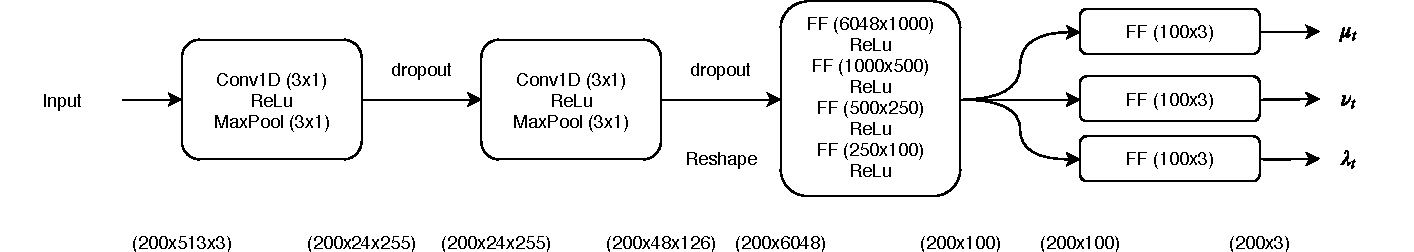
\includegraphics[width=\linewidth]{mirage/cnn.pdf}
    \end{sidecaption}
\end{figure}

\mynewline
As shown in~\cref{fig:lantern:cnn}, the architecture consists of two convolutional modules made of a one-dimensional convolutional layer (1DConv) followed by max-pooling along the frequencies, followed by \ac{ReLU} activation function and batch-normalization.
The second part consists of a cascade of fully connected feed-forward (FF) layers.
In order to perform 1D-convolution ond the right dimension, we re-arranged the input so that the each of features $\klist{ \ild, \kRe\set{\ipd}, \kIm\set{\ipd}}$ is considered as channel for the 1DConv.
After each layer a dropout probability $p_\text{do} = 0.3$ is applied.

\mynewline
In the \ac{MLP} model presented above in the previous section, the output consisted only in the \acp{TDOA} $V$.
However, to build a local angular spectrum, suitable for the \ac{SRP-PHAT}-like algorithm, both means and variances are needed.
Rather than identify these variances with the prediction errors, we explicitly modify the \ac{CNN} model to estimated them\sidenote{
    This idea is similar to the one proposed by Bishop in \ac{MDN} in \citeonly{bishop1994mixture}
    where the output of a neural network parametrizes a Gaussian mixture model.
}.
The main idea behind this design choice is that the learning model can assess its prediction quality.
This approach can be related to existing (Bayesian) data-fusion frameworks, but this direction wav not considered in this work.
\newcommand{\setTDOA}{\ensuremath{\set{\mathtt{TDOA}, \mathtt{iTDOA}, \mathtt{TDOE}}}}
\\To this end, we modify the output of the network to output mean and variances, namely
$V_{\calN} = \set{\mu_{\tau_t}, \sigma^2_{\tau_t}}$
for $t = \setTDOA$.
Moreover, we assume that conditional probability of observing the one of the \ac{TDOA} $\tau_t$ for $t \in \setTDOA$ given the observation $\xi$ in the batch $\Xi$, follows a Gaussian distribution, namely
\begin{equation}
    p(\tau_t \mid  \Xi ; \theta) \sim \calN\kparen{\mu_{\tau_t}(\xi_b;\theta), \sigma^2_{\tau_t}(\xi_b;\theta)}
\end{equation}
where the variance
and the the training loss function
 of~\cref{eq:mirage:mlploss}
\begin{equation}\label{subsec:mirage:mlpcost}
    \calL(V, \hat{V)} = \frac{1}{3} \sum_{b}  \powerOf{\tau_{\mathtt{TDOA}, b} - \hat{\tau}_{\mathtt{TDOA}, b}}
                                            + \powerOf{\tau_{\mathtt{iTDOA}, b} - \hat{\tau}_{\mathtt{iTDOA}, b}}
                                            + \powerOf{\tau_{\mathtt{TDOE}, b} - \hat{\tau}_{\mathtt{TDOE}, b}}
\end{equation}


\newthought{The proposed novel loss function} is the negative Student-T log-likelihood, which is implemented as follows:

\begin{equation}
\begin{split}
\mathcal{L}(\Theta) =& \sum_{x \in B} \sum_{t \in V}\ \dfrac{1}{2} \log (\nu_t\pi_t)
                        + \dfrac{1}{2} \log(\lambda_t^2)
                        - \log  \Gamma \left( \dfrac{\nu_t+1}{2} \right)\\
                    &    + \log  \Gamma \left( \dfrac{\nu_t}{2} \right)
                        + \dfrac{\nu_t+1}{2}
                        \log \left( 1  + \dfrac{\norm{\mu_t, x_i)}}{\nu_t \lambda_t^2} \right)\\
\end{split}
\end{equation}

where $\Theta$ are the CNN parameters and $\Gamma$ is the Gamma function. The summation over $i$ corresponds to the sum among of all the sample $x$ of the batch $B$. and the summation over $t$ corresponds to the sum among the three quantities in V (TDOA, iTDOA, TDOE). It follows that for each each input the network will return the parameters of 3 Student-T distribution ($\mu_t, \nu_t, \lambda_t$) for each variable $t = { \text{TDOA}, \text{iTDOA}, \text{TDOE} }$. Hereafter we denote with $V_{\mathcal{ST}}$ the set of the 9 network outputs.
We use the Adam optimizer ant the normalized root mean square error (nRMSE) is taken as validation metric (see Section~\ref{subsec:eval_synth_tdoa}). The network is manually tuned on a validation set to find the best combination of number of hidden layers and their sizes
Once an estimate $\hat{V_\mathcal{ST}}$ of the parameters of the 3 distribution is returned by the CNN, they are converted to synthetic local angular spectra and passed to an SRP-PHAT method together with the relative positions of true and image microphones which are assumed known. We call this algorithm MIRAGE. The synthetic local angular spectra consist of Student-t distribution with parameters $\mu, \nu$ and $\lambda$.
and $V \in \mathbb{R}^3$ as output parameters.


We use a simple fully-connected DNN architecture consisting of a $D$-dimensional input layer,
a $3$-dimensional output layer, and 3 fully connected hidden layers with respective input
sizes $500$, $300$ and $50$. Rectified linear unit (ReLU)
activation functions are used except at the output layer,
and each hidden layer has a dropout probability $p_\text{do} = 0.3$.
We use the mean square error loss function for training and the Adam optimizer \cite{kingma2014adam}.
The normalized root mean square error (nRMSE) is taken as validation
metric\footnote{The nRMSE takes values between $0$ (perfect fit) and $\infty$ (bad fit).
If it is equal to $1$, then the prediction is no better than a constant.}.
The network is manually tuned on a validation set to find the best combination of number of hidden layers, their sizes and $p_\text{do}$.
Once time delay estimates $\hat{V}$ are returned by the DNN, they are converted to synthetic
local angular spectra and passed to $\Psi_\text{SRP}$ (See Sec. \cref{subsec:mirage:2D-SSL})
together with the relative positions of true and image microphones which are assumed known.
We call this algorithm MIRAGE. The synthetic local angular spectra consist of Gaussians
centered at $\hat{V}$ and with variances equal to the prediction errors made by
the DNN on the validation set.

For training and validation, the RIRs are convolved with 1 sec of white-noise with additional noise with SNR in $(0,20)$ dB.
All signals and RIRs are sampled at $16$ kHz. The STFT is performed on $1024$ point with $50\%$ overlap. Finally the features are computed as in~\eqref{eq:features} yielding a vector of size $D = 1534$ for each observation.
While we validate the CNN on a portion of the dataset in a \textit{holdout} fashion, the test is conducted on 200 new RIRs convolved with both speech utterances.
This set is generated similarly to the training and validation sets. Moreover the recordings are perturbed by external white noise as in the training set. The speech signals are normalized speech utterances of various lengths (from $1$ s to $6$ s), randomly selected from the TIMIT corpus.
A re-implement version of SRP-PHAT is used to aggregate local angular spectra obtained from the DNN's output and as a baseline.
 However the original MATLAB code for SRP-PHAT can be found at \url{http://bass-db.gforge.inria.fr/bss_locate/}. A sphere sampling with $1$ degree resolution and coordinates $\theta \in [-179, 180]$ and $\phi \in [0, 90]$ degrees is used for the DOA search.


\section{Conclusion and perspective}

\newthought{Towards the case $\numEchs > 2$}

\newthought{Better features: \RTF/}

\newthought{Better architecture: Physical-based learning and unfolding}


% \begin{table}[ht!]
%     \begin{sidecaption}[Echo estimation with MIRAGE results]{%
%         Normalize root mean squared error for TDOA estimation and mean angular error in ${}^\circ$ (with accuracies ($\%$))
%         for AOA estimation with $\ang{10}$ and $\ang{20}$ angular tolerance.
%     }[tab:mirage:tdoas-aoa]
%     \centering
%     \footnotesize
%     %\scriptsize
%     \begin{tabular}{cl|ccc|cc}
%     \toprule
%                 &         &          & nRMSE        &                   &\multicolumn{2}{c}{ACCURACY}  \\
%                 & Input   &    \scriptsize{TDOA}  	&   \scriptsize{iTDOA} 		 &     \scriptsize{TDOE} 		 & $\theta<\ang{10}$ &  $\theta<\ang{20}$ \\
%     \midrule
%     MIRAGE      &   wn    & 0.18    & 0.28  & 0.25 	& 4.10 (77)	& 5.97 (97) \\
%     MIRAGE      &   wn+n  & 0.68    & 0.69  & 0.89 	& 5.00 (26)	& 9.89 (54) \\
%     MIRAGE      &   sp    & 0.31    & 0.34  & 0.56  & 4.83 (63)	& 7.26 (82) \\
%     MIRAGE      &   sp+n  & 0.99    & 0.98  & 1.48 	& 4.60 (16)	& 9.88 (35) \\
%     GCC-PHAT    &   wn    & 0.21    & -     & -		& 4.22 (81) & 6.19 (97) \\
%     GCC-PHAT    &   wn+n  & 0.68    & -     & -		& 4.03 (65) & 5.34 (83) \\
%     GCC-PHAT    &   sp 	  & 0.32    & -     & -		& 4.08 (82) & 5.34 (97) \\
%     GCC-PHAT    &   sp+n  & 1.38    & -     & -		& 4.70 (19) & 8.38 (32) \\
%     \bottomrule
%     \end{tabular}
%     \end{sidecaption}
% \end{table}
% \chapter{\library{dEchorate}: Datasets for Acoustic Echo Estimation}\label{ch:dechorate}

\openepigraph{Once you've been alone\\
And everybody knows\\
Work begins alone}{Strapping Young Lad, \textit{Monument}}


\vspace{-2.5em}
\newthought{Synopsis} \marginpar{%
\footnotesize
\textbf{Keywords:} Room impulse response, early reflection, acoustic echoes, audio database, microphone arrays.
\\\textbf{Resources:}
\begin{itemize}
    \item \href{https://github.com/Chutlhu/DechorateDB}{Code repository}
    \item \href{https://github.com/Chutlhu/DechorateDB}{Dataset data}
\end{itemize}
} \synopsisChDechorate


\mynewline
The material presented in the chapter is the result of a work done while visiting prof. Sharon Gannot and ing. Pinchas Tandeitnik at the Bar'Ilan University, Israel.
The work described here, together with its continuation described in~\cref{ch:dechorateapp} will be submitted as a journal article to the EURASIP special edition \textit{Data-driven Audio Signal Processing: Methods and Apps}.


\section{Introduction}\label{sec:dechorate:intro}
As discussed~\cref{sec:estimation:datasets}, many \acp{RIR} datasets are available online.
However, most of them are specifically designed for applications either to \acf{SE} or to \acf{RooGE}.
The main common drawback of these datasets in that they can not be easily used for other tasks than the one which they were designed for.
In particular, \SE/-oriented datasets lack of a proper annotation of echoes in the \acp{RIR} or the absolute position of objects inside the room.
Conversely, datasets for \RooGE/ typically features design choices which are not suitable for many \SE/ application, involving the positioning of microphone(s) and source(s).
\dEchorate{} was designed to fill this gap: a fully calibrated multichannel \ac{RIR} database with accurate annotation of the geometry and echoes in different configurations of a cuboid rooms with varying wall acoustic profiles.
The database currently features 1800 annotated \acp{RIR} obtained from 6 arrays of 5 microphones each, 6 sound sources in 10 different acoustic conditions.
All the measurements were realized in the acoustic lab at Bar-Ilan university following a consolidated protocol previously established for the realization of two other multichannel \acp{RIR} databases:
the \href{http://www.eng.biu.ac.il/~gannot/RIR_DATABASE/}{BIU's Impulse Response Database\ExternalLink} \citeonly{Hadad2014multichannel} gathering \acp{RIR} of different reverberation levels sensed by uniform linear arrays (ULAs);
and \href{https://asap.ite.tul.cz/downloads/MIRaGe/}{\library{MIRaGE}\ExternalLink}~\citeonly{cmejla2019mirage} providing a set of measurements of a source placed on a dense position grid.
\dEchorate{} is designed for \acf{AER} with linear arrays, and is more generally aimed at analyzing and benchmarking RooGE and echo-aware signal processing methods on real data.
In particular, it can be used to assess robustness against the number of reflectors, the reverberation time, additive spatially-diffuse noise and non-ideal frequency and directive characteristics of microphone-source pairs and surfaces in a controlled way.
Due to the amount of data and recording conditions, it could also be used to train machine learning models or as a reference to improve \ac{RIR} simulators.
The database is accompanied with a Python toolbox that can be used to process and visualize the data, to perform analysis or to annotate new datasets.

\begin{figure}[t]
    \begin{fullwidth}
        \centering
        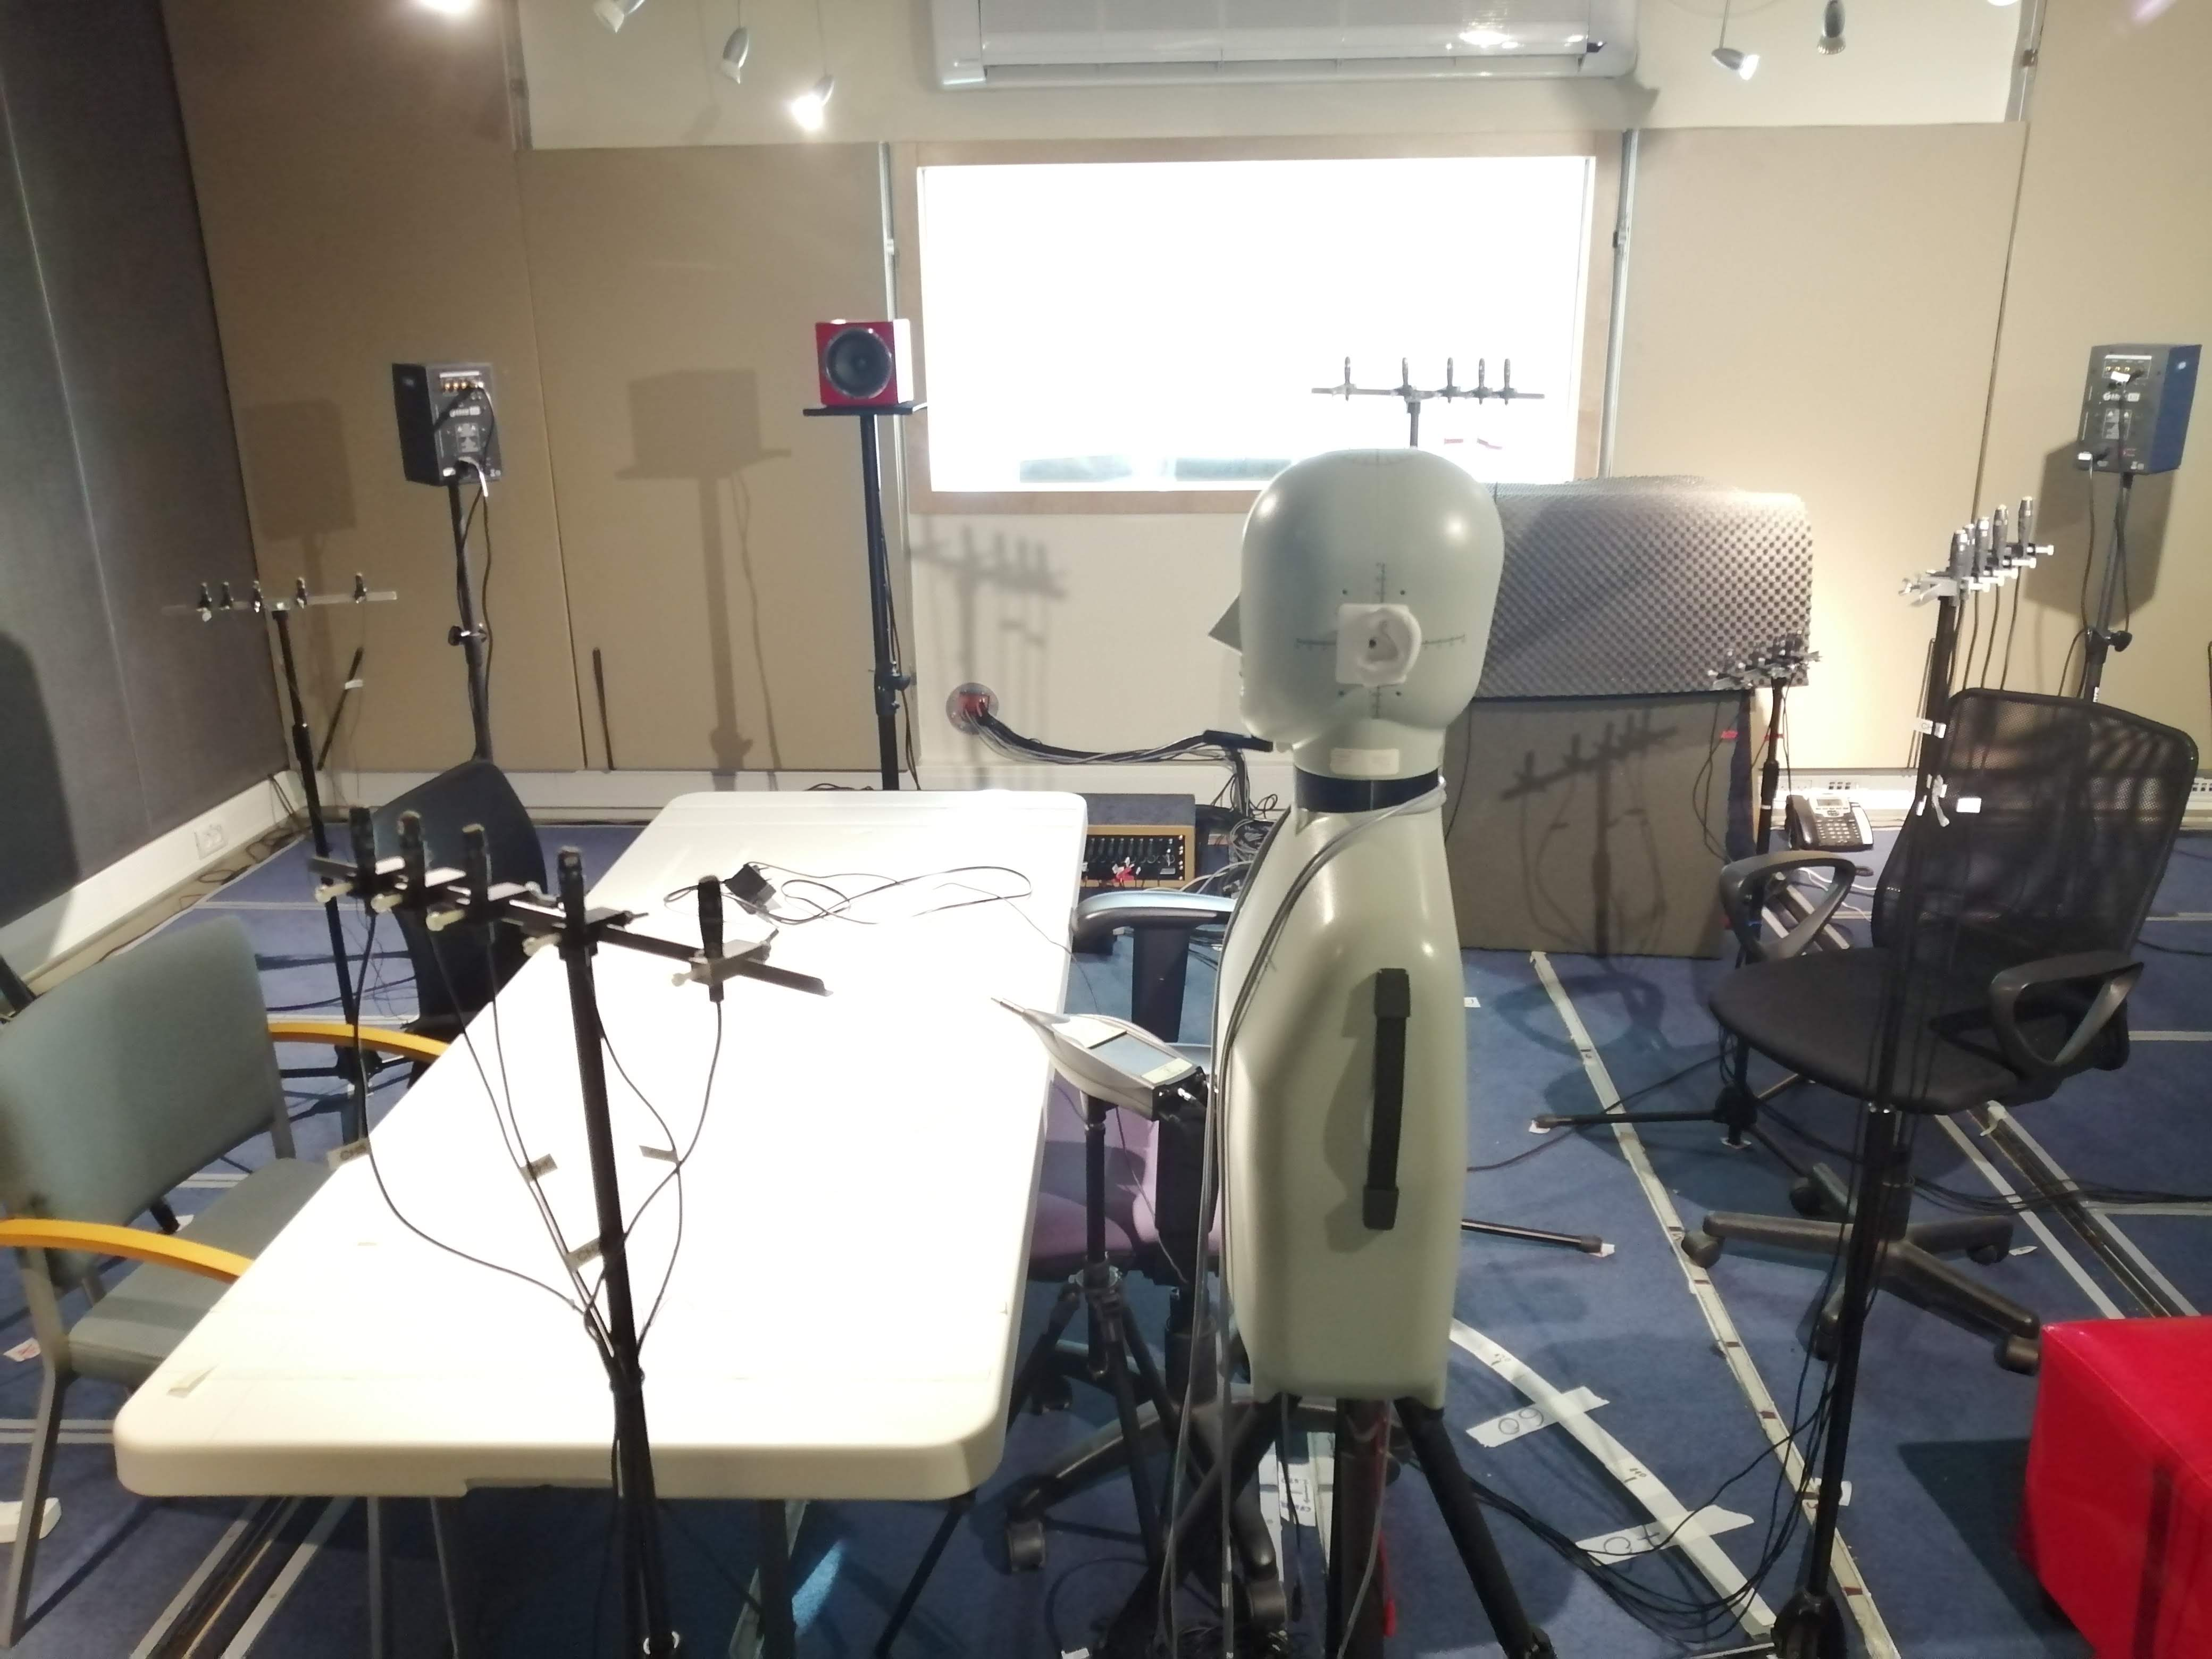
\includegraphics[trim={0 0 0 10em},clip,width=\linewidth]{dechorate/fornitures.jpg}
        \caption{Broad-view picture of the acoustic lab at Bar-Ilan university.}
        \label{fig:dechorate:room}
    \end{fullwidth}
\end{figure}


\section{Database realization}
\subsection{Recording setup}
The recording setup is situated in a cuboid room with dimension 6~m $\times$ 6~m $\times$ 2.4~m.
The 6 facets of the room (walls, ceiling, floor) are covered by acoustic panels allowing controllable reverberation time ($\RT$).
We placed $4$ directional loudspeakers (direct sources) facing the center of the room and $30$ microphones mounted on 6 non-uniform linear arrays (nULA) of 5 sensors each.
An additional channel is used for the loop-back signal, which serves to compute the time of emission and detect errors.
Each loudspeaker and each array was positioned close to one of the walls in such a way that the nature of the strongest echo can be easily identified.
Moreover, their positioning was chosen to cover a wide distribution of source-to-receiver distances, hence, a wide range of direct-to-reverberant ratios (\ac{DRR}).
Further, $2$ more loudspeakers were positioned pointing towards the walls (indirect sources).
This was done to study the case of early reflections being stronger than the direct-path.
Each linear microphone array consists of 5 microphones with non-uniform inter-microphone spacings of $[4, 5, 7.5, 10]$~cm\sidenote{
    \scriptsize\ie/
    $[-12.25, -8.25, $ $-3.25, 3.25, 13.25]$ cm w.r.t the barycenter}.
Each array is steered towards a different vertical edge of the room for calibration and reproducibility purposes.


\begin{table}[h]
    \begin{sidecaption}[]{
        Technical specification of the measurements equipment used in the recordings.
        }[tab:dechorate:room_equipment]
        \centering
        \small
        \begin{table}[]
    \centering
    \small
    \begin{tabular}{ll}
        \toprule
         Loudspeakers   & (directional, direct) $4 \times$ Avanton\\
                        & (directional, indirect) $2 \times$ Avanton\\
                        & (omnidirectional) $1 \times$ B\&G\\
                        & (babble noise) $4 \times$ 6301bx Fostex\\
         \hline
         Microphones    & $30 \times$ AKG CK32\\
         Array          & $6 \times$ nULA (5 mics each, handcrafted)\\
         \hline
         A/D Converter  & ANDIAMO.MC\\
         \hline
         Indoor Positioning & Marvelmind Starter Set HW v4.9\\
         \bottomrule
    \end{tabular}
    \caption{Measurements equipment.}
    \label{tab:room_equipment}
\end{table}
    \end{sidecaption}
\end{table}

\begin{figure}[b]
    \begin{sidecaption}[]{
        Illustration of the recording setup - top view.
        }[fig:dechorate:2D]
        \centering
        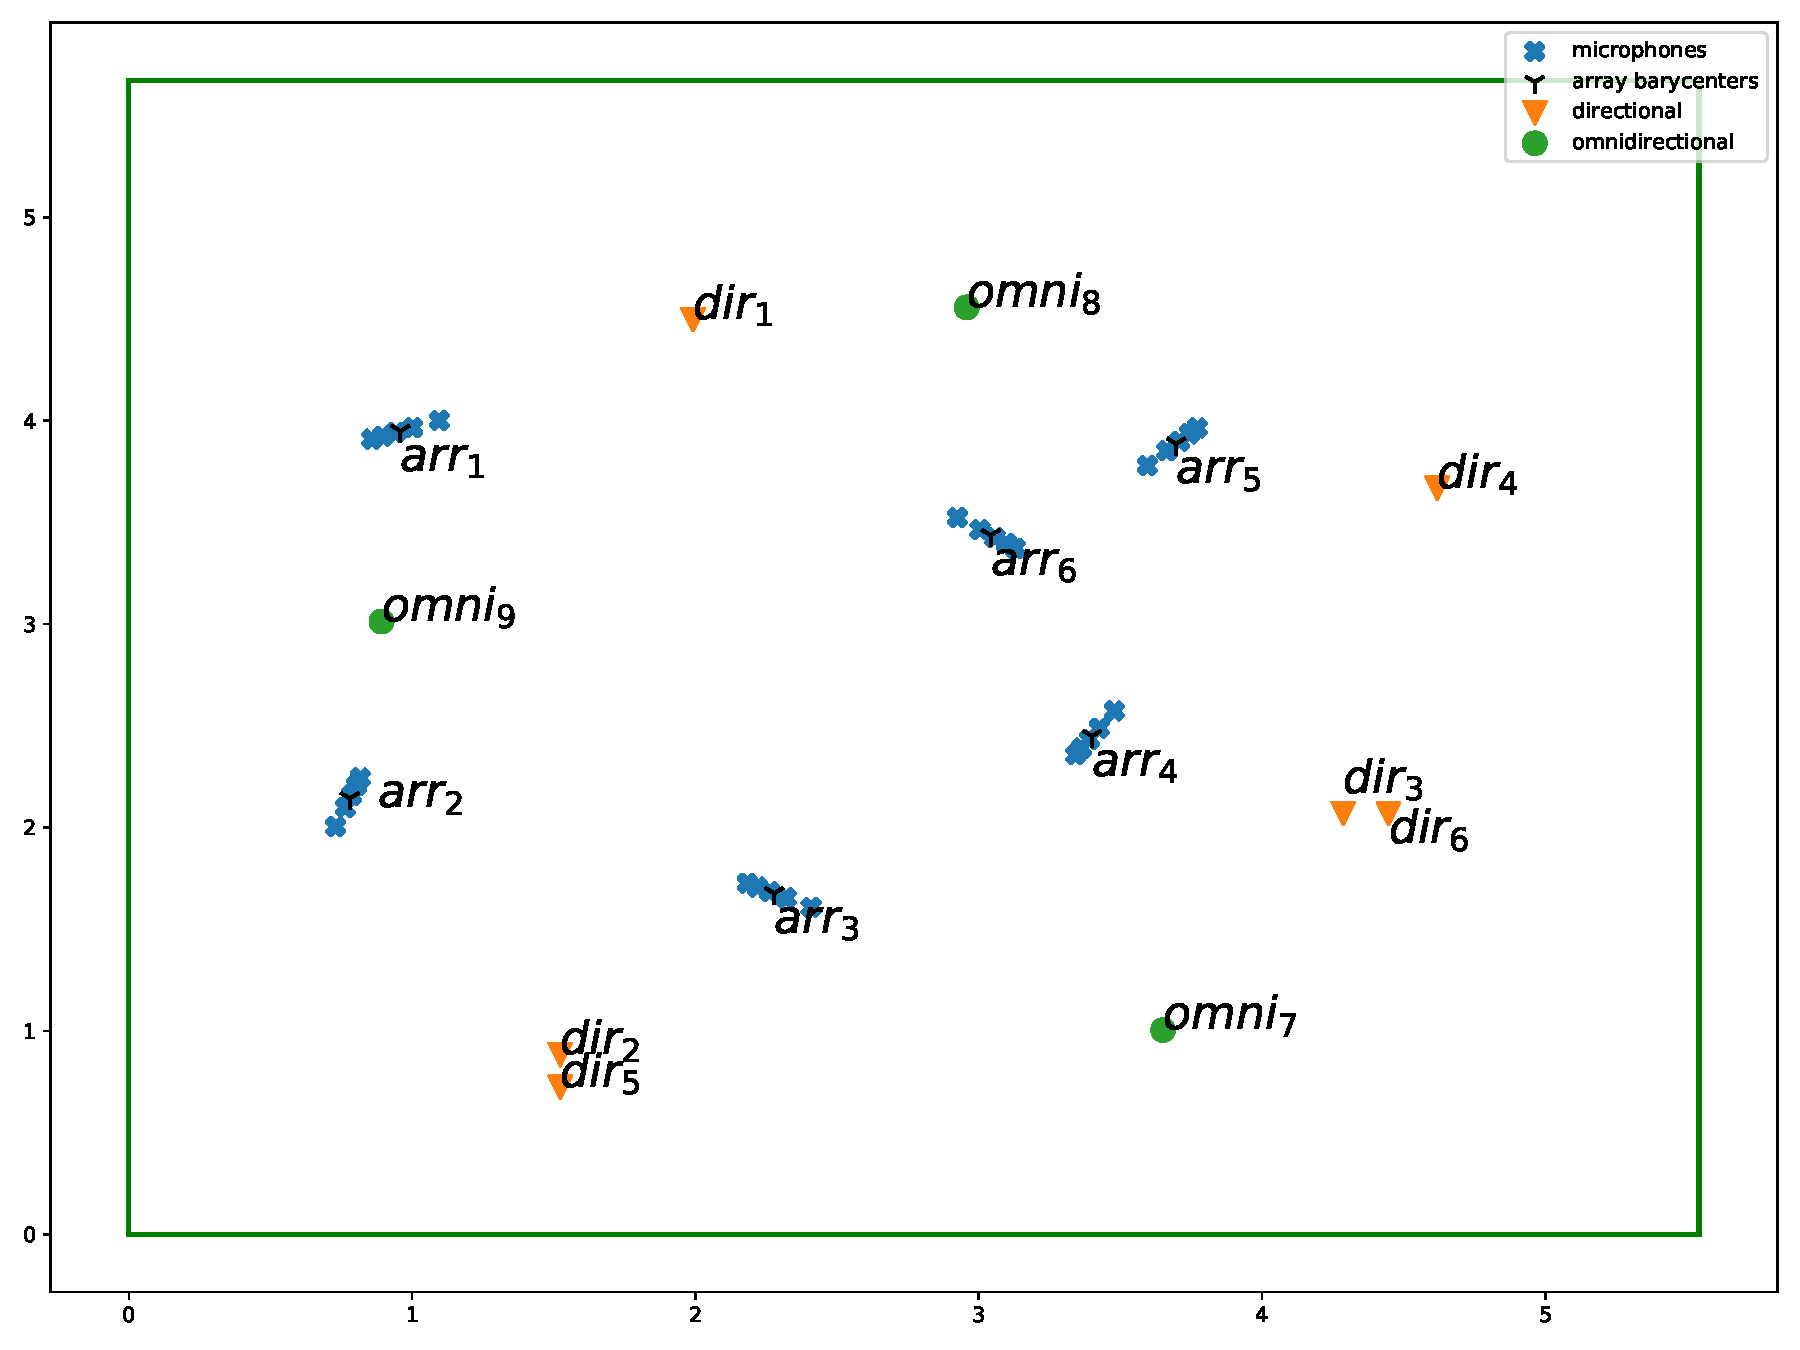
\includegraphics[width=0.8\linewidth]{figures/dechorate/positioning2D_xy.pdf}
    \end{sidecaption}
\end{figure}

\begin{figure}[t]
    \begin{fullwidth}
    \centering
    \subfloat[mu_spkr][Overall setup]{
        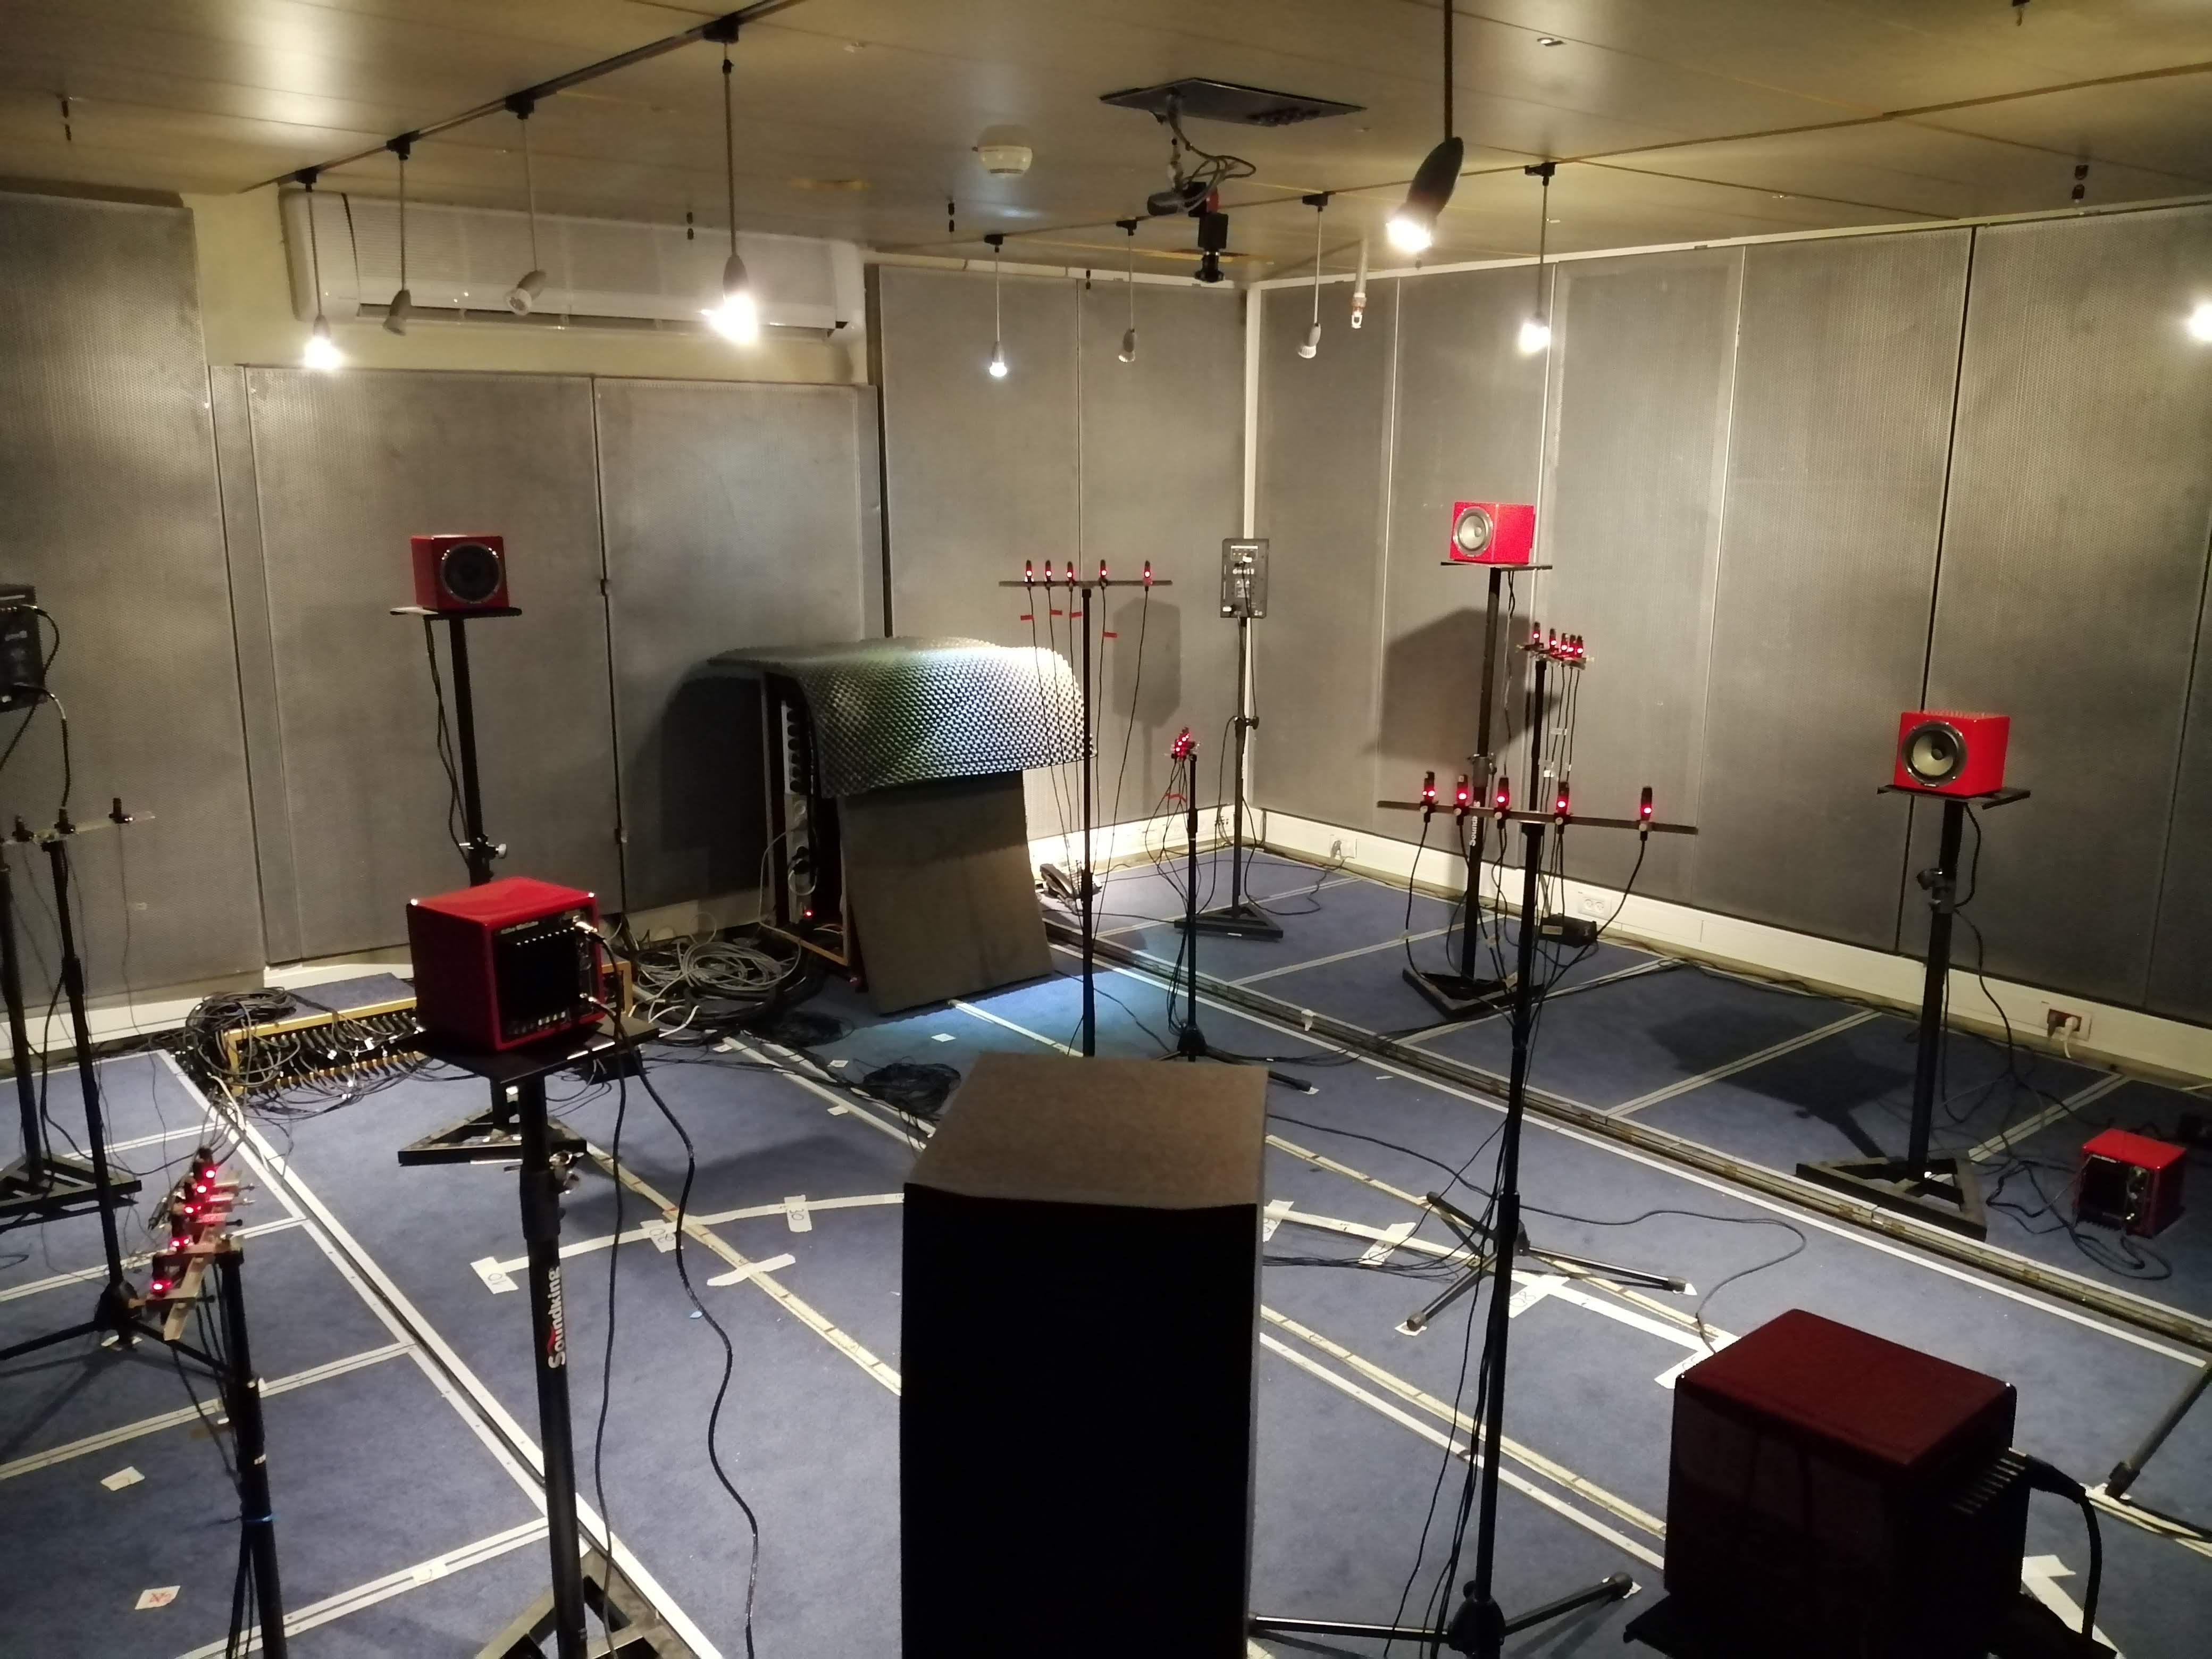
\includegraphics[width=0.325\textwidth]{figures/dechorate/recording_setup}}
    %
    \subfloat[mu_spkr][Microphone array]{
        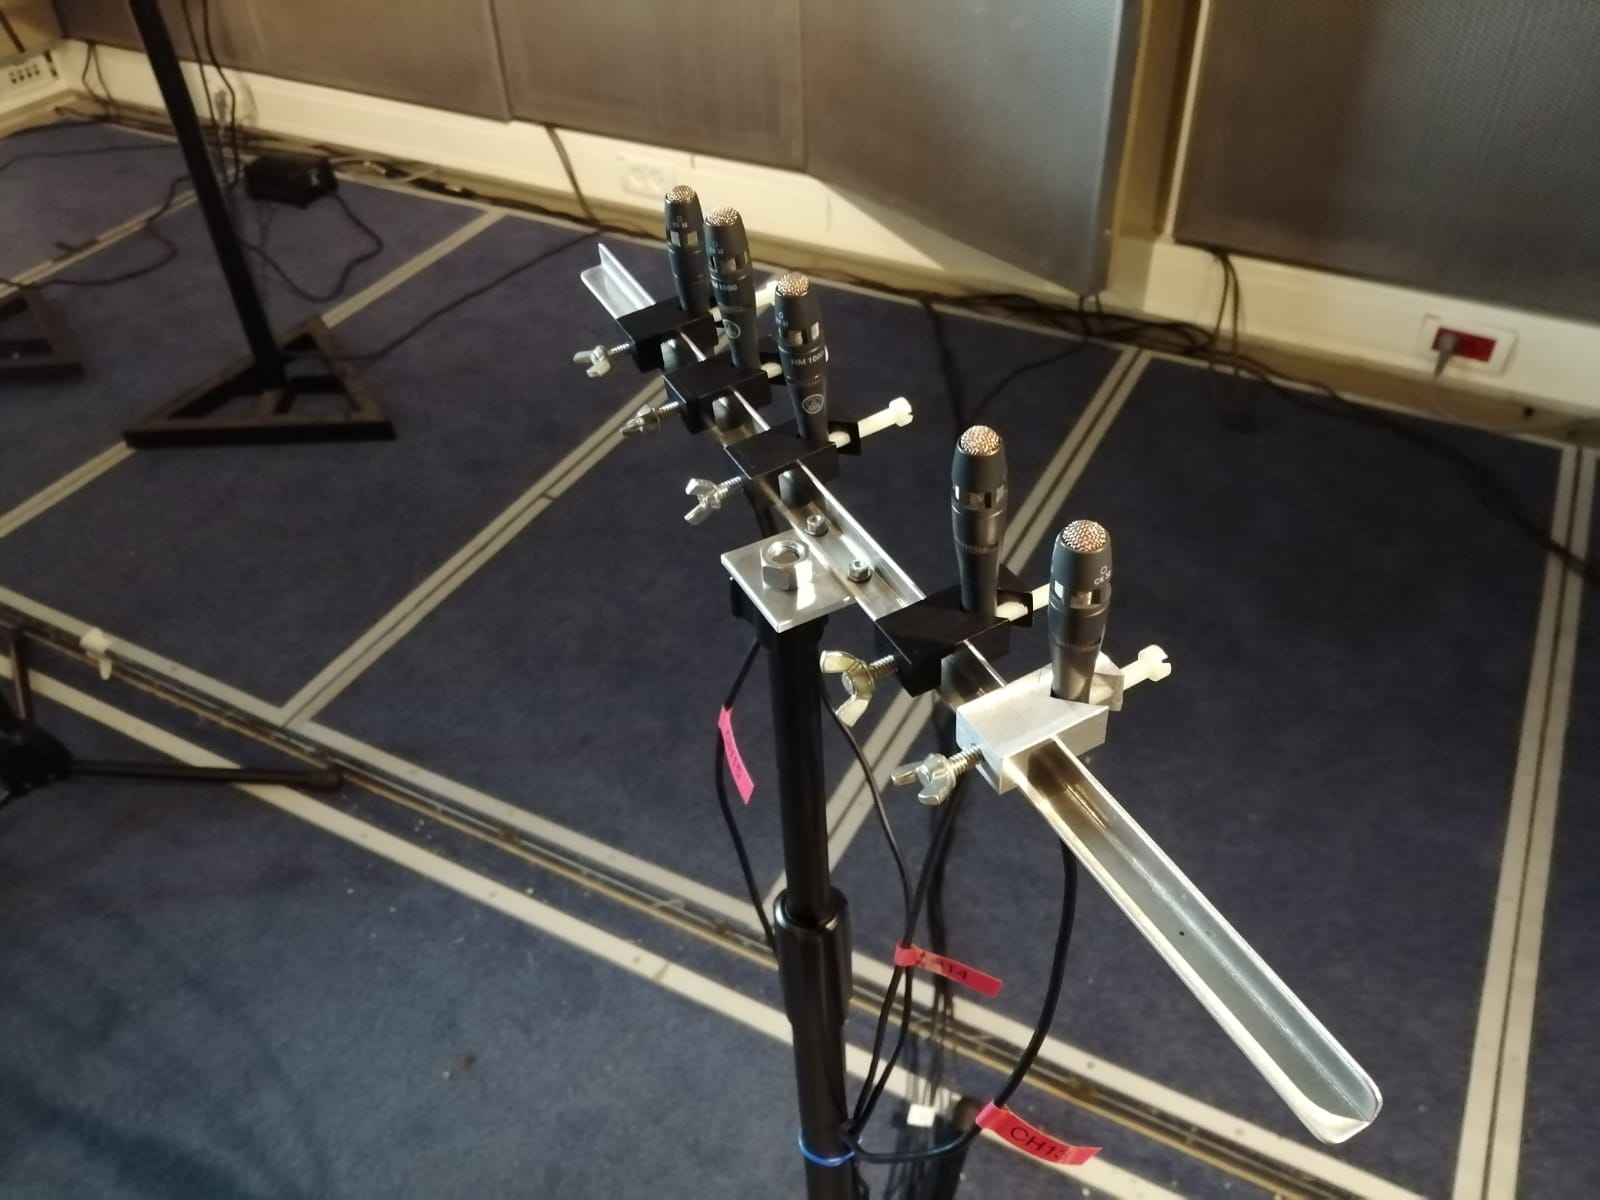
\includegraphics[width=0.325\textwidth]{figures/dechorate/mic}}
    %
    \subfloat[mu_univ][Revolving panels]{
            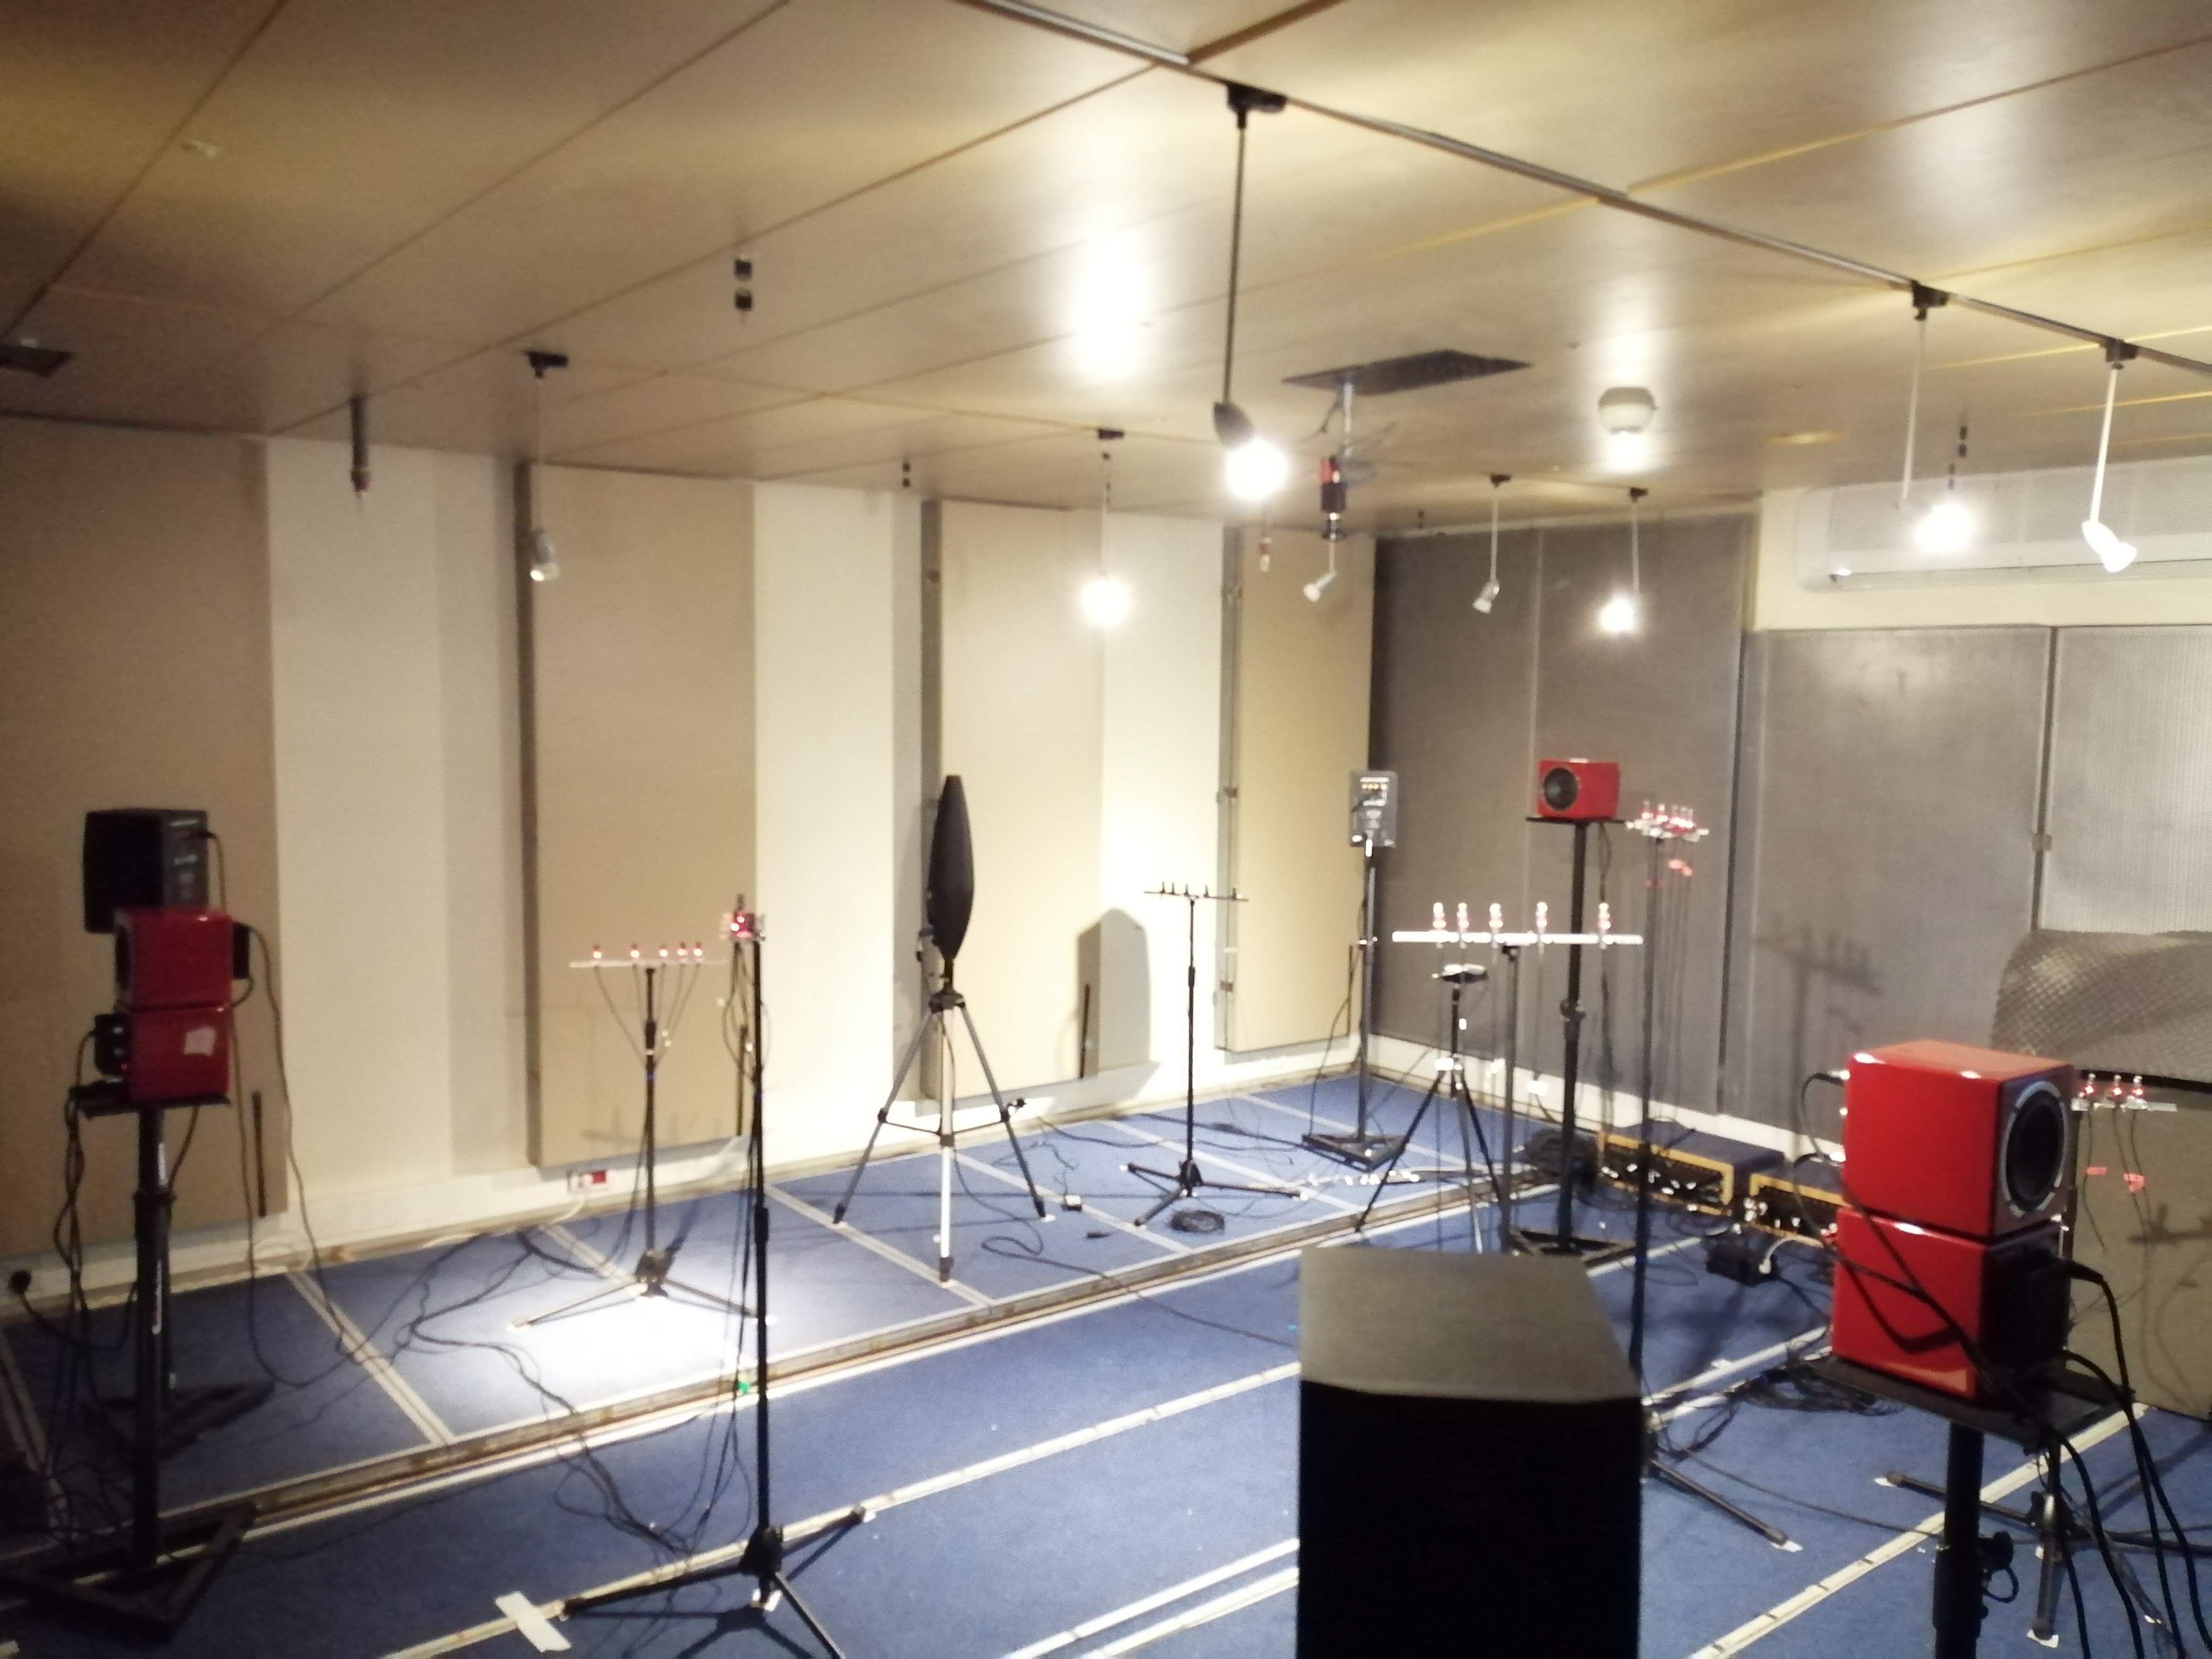
\includegraphics[width=0.325\textwidth]{figures/dechorate/panels}}
    \label{fig:dechorate:setup}
    \caption{Picture of the acoustic lab. From left to right: the overall setup, one microphone array, the setup with revolved panels.}
    \end{fullwidth}
\end{figure}

\subsection{Measurements}
The main feature of this room is the capability to change the acoustic profile of each of its facet by flipping double-sided panels with one reflective and one absorbing face.
This allows to achieve precise values of $\RT$ that range from 0.1 to almost 1~second.
In this dataset the panels of the floor were kept always absorbent.

\mynewline
Two types of sessions were considered, namely, \textit{one-hot} and \textit{incremental}.
For the first type, a single facet was placed in reflective mode while all the others were kept absorbent.
For the second type, starting from fully-absorbent mode, facets were progressively switched to reflective mode one after the other until all but the floor were reflective, as shown in Table \ref{tab:dechorate:wallcoding}.

\mynewline
The dataset features an extra recording session.
For this session, office furnitures were positioned in the room to simulate a typical meeting room with chairs and tables (See~\cref{fig:dechorate:room}).
Theses recordings will be used in future works for asserting the robustness of echo-aware methods in a more realistic scenario?.

\begin{table}[h]
    \begin{sidecaption}[]{
        Surface coding in the dataset: each binary digit indicates if the surface is absorbent ($\mathtt{0}$, \xmark ) or reflective ($\mathtt{1}$, \cmark).
        }[tab:dechorate:wallcoding]
        \centering
        \small
        \begin{tabular}{cc|cccccc}
\toprule
& Surfaces:                 & Floor                 & Ceiling               & West                  & South                 & East                  & North                 \\ \hline
\multicolumn{1}{c}{\multirow{5}{*}{\rotatebox{90}{one-hot}}} & $\mathtt{000000}$                   & \xmark & \xmark & \xmark & \xmark & \xmark & \xmark \\
& $\mathtt{010000}$                    & \xmark & \cmark & \xmark & \xmark & \xmark & \xmark \\
& $\mathtt{001000}$                    & \xmark & \xmark & \cmark & \xmark & \xmark & \xmark \\
& \multicolumn{1}{c|}{$\dots$}  & \multicolumn{6}{c}{$\dots$} \\
& $\mathtt{000001}$                    & \xmark & \xmark & \xmark & \xmark & \xmark & \cmark \\
\multicolumn{1}{c}{\multirow{4}{*}{\rotatebox{90}{incremental}}} & $\mathtt{011000}$                    & \xmark & \cmark & \cmark & \xmark & \xmark & \xmark \\
& $\mathtt{011100}$                    & \xmark & \cmark & \cmark & \cmark & \xmark & \xmark \\
& \multicolumn{1}{c|}{$\dots$} & \multicolumn{6}{c}{$\dots$}  \\
& $\mathtt{011111}$                    & \xmark & \cmark & \cmark & \cmark & \cmark & \cmark \\
\bottomrule
\end{tabular}


    \end{sidecaption}
\end{table}


\mynewline
For each room configuration and loudspeaker, three different excitation signals were played and recorded in sequence: chirps, white noise and speech utterances.
The former consists in a repetition of 3 \acf{ESS} signals of duration 10~seconds and frequency range from 100 Hz to 14~kHz interspersed with 2~seconds of silence.
Such frequency range was chosen to match the characteristics of the loudspeakers.
To prevent rapid phase changes and ``popping'' effects, the signals were linearly faded in and out over 0.2~seconds with a Tuckey taper window\sidenote{
    The code to generate the reference signals and to process them is available togheter with the data.
    Such code is based on the \href{https://github.com/maj4e/pyrirtool}{\library{pyrirtool}\ExternalLink} Python library.
}.
Secondly, 10~seconds bursts of white noise and 3 anechoic speech utterances from the \WSJ/ dataset \citeonly{Paul1992design} were reproduced in the room.
Through all the recordings, at least 40~dB of sound dynamic range was asserted and a room temperature of $\ang{24} \pm \ang{0.5}$ and humidity of 80\% were registered.
Moreover, 1~minute of \textit{room tone} (silence) and 4~minutes of diffuse babble noise were recorded for each session.
The latter was simulated by transmitting different chunks of the same single-channel babble noise recording from additional loudspeakers facing the four corners of the room.

\mynewline
All the microphone signals were synchronously acquired and digitally converted to 48 kHz with 32 bits/sample using the equipment listed in Table~\ref{tab:dechorate:room_equipment}. The polarity of each microphone was registered by clapping a book in the middle of the room.

\section{Dataset annotation}\label{sec:annotation}
\acp{RIR} are estimated with the ESS technique \citeonly{farina2007advancements} at 48 kHz:
the signal of a microphone recording an \ESS/ source is deconvolved by division in the frequency domain.
Notice that the \ac{FT} of the \ESS/ signal is available in closed form and we used its \ac{DFT} approximation.

\subsection{RIRs annotation}
The objective of this database is to feature off-grid annotations in the ``geometrical space'', namely microphone, wall and source positions, \textit{fully consistent} with annotations in the ``signal space'', namely the echo timings within the \acp{RIR}.
This results is achieved as follows:
\begin{enumerate}[label=(\roman*)]
    \item \label{it:decharate:ips} First, the ground-truth position of array and source centres are acquired via a Beacon indoor positioning system ($\bIPS$).
    This system consists in 4 stationary bases positioned at the corners of the ceiling and a movable probe used for measurements which can be located within errors of $\pm2$~cm.
    The elements of this system are shown in~\cref{fig:dechorate:bips}.
    \marginpar{
        \centering
        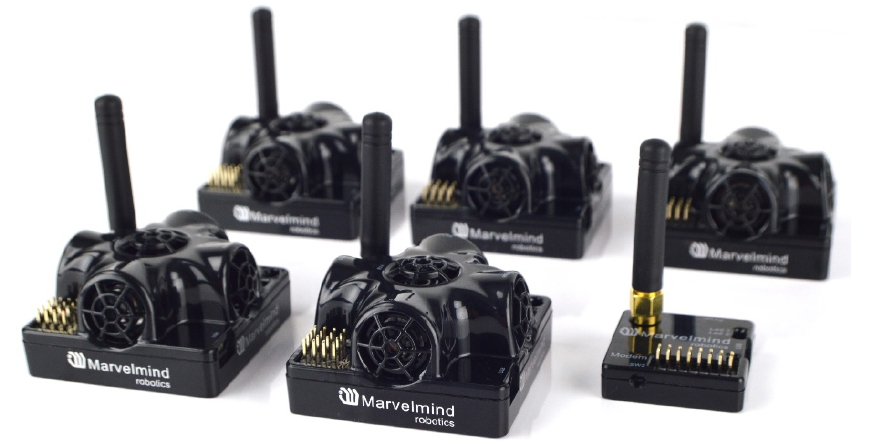
\includegraphics[width=\linewidth]{dechorate/IPSbeacon.jpg}
        \captionof{figure}{
            Picture of the Beacon indoor positioning system used for measuring array and loudspeaker 3D position.
        }
        \label{fig:dechorate:bips}
    }
    \item \label{it:decharate:not} The estimated \acp{RIR} are superimposed on synthetic \acp{RIR} computed with the \acf{ISM} from the geometry obtained in the previous step.
    A Python GUI\sidenote{This GUI is available in the dataset package.} (showed in~\cref{fig:dechorate:labelling_tools}), was used to manually tune a peak finder and label the echoes corresponding to found peaks, that is, annotate their positions and their corresponding image source position and wall label..

    \item \label{it:decharate:mds} By solving a simple \acf{MDS} problem \citeonly{dokmanic2015relax,crocco2016estimation, Plinge2016acoustic}, refined microphone and source positions were computed.
    The non-convexity of the problem was alleviated by using a good initialization (obtained at the previous step), by the high SNR of the measurements and, later, by including the additional image sources in the formulation.
    The prior information about the arrays' structures reduced the number of variables of the problem, leaving the 3D positions of the sources and of the arrays' barycenters in addition to the the arrays' tilt on the azimuthal plane.

    \item \label{it:decharate:lat} By employing a multilateration algorithm \citeonly{Beck2008ExactProblems}, where the positions of one microphone per array serve as anchors and the \TOAs/ are converted into distances, it was possible to localize image sources along side with the real sources.
    This step will be further discussed in~\cref{ch:dechorateapp}.
\end{enumerate}
Knowing the geometry of the recording room, we were able to manually label the echoes by iterating through steps \ref{it:decharate:not}, \ref{it:decharate:mds} and \ref{it:decharate:lat}.

\newthought{The final geometrical and signal annotation} was chosen as a compromise between the $\bIPS$ measurements and the \ac{MDS} output.
While the former ones are noisy but consistent with the scene's geometry, the latter ones matches the \TOAs/ but not necessarily the physical world.
In particular, geometrical ambiguities such as global rotation, translation and up-down flips were observed.
Instead of manually correcting this error, we modified the original problem from using only the direct path distances ($\dMDS$) to considering the  image sources' \TOA/ of the ceiling as well in the cost function ($\dcMDS$).
Table~\ref{tab:dechorate:res_mds} shows numerically the \textit{mismatch} (in cm) between the geometric space (defined by the $\bIPS$ measurements) and the signal space (the one defined by the echo timings, converted in cm).
To better quantify it, we introduce here a \textit{goodness of match} (GoM) metric: it measures the fraction of (first-order) echo timings annotated in the \acp{RIR} matching the annotation produced by the geometry within a threshold.
Including the ceiling information, $\dcMDS$ produces a geometrical configuration which has a small mismatch (0.41~cm in average) in both the signal \textit{and} geometric spaces with $98.1\%$ of matching first order echoes within a 1~ms threshold.
Nevertheless, it is interesting to see that the $\bIPS$ measurements produce a good but less precise annotation.

\begin{table}[]
    \begin{sidecaption}[]{
        Mismatch between geometric measurements and signal measurements in terms of maximum (Max.), average (Avg.) and standard deviation (Std) of absolute mismatch in centimeters. The \textit{goodness of match} (GoM) between the signal and geometrical measurements is reported as fraction of matching echo timing for different threshold in milliseconds.
        }[tab:dechorate:res_mds]
        \centering
        \small
        \begin{tabular}{lllll}
\toprule
& Metrics        & $\bIPS$               & $\dMDS$          & $\dcMDS$          \\
\midrule
\multicolumn{1}{c}{\multirow{2}{*}{\rotatebox{90}{\footnotesize Geom.}}}
&   Max.             & -            & $6.1$         & $1.07$        \\
&   Avg.$\pm$Std.    & -            & $1.8\pm1.4$    & $0.39\pm0.2$  \\
% \rule{0pt}{0.1em}\\
\midrule
\multicolumn{1}{c}{\multirow{2}{*}{\rotatebox{90}{\footnotesize Signal}}}
&   Max.          & $5.86$         & $1.20$         & $1.86$       \\
&   Avg.$\pm$Std. & $1.85\pm 1.5$  & $0.16\pm0.2$   & $0.41\pm0.3$ \\
% \rule{0pt}{0.1em}\\
\midrule
\multicolumn{1}{c}{\multirow{3}{*}{\rotatebox{90}{\footnotesize Mismatch}}}
&  GoM (1.0 ms)   & $97.9 \%$      & $93.4 \%$      & $98.1 \%$ \\
&  GoM (0.1 ms)   & $26.6 \%$      & $44.8 \%$      & $53.1 \%$ \\
&  GoM (0.05 ms)  & $12.5 \%$      & $14.4 \%$      & $30.2 \%$ \\
\bottomrule
\end{tabular}

    \end{sidecaption}
\end{table}

\subsection{Other tools for RIRs annotation}
Finally, we want to mention that the following tools and techniques were found helpful in annotating the echoes.

\newthought{The \library{skyline} visualization} consists in presenting multiple \acp{RIR} as an image, such that the wavefronts corresponding to echoes can be highlighted \citeonly{Baba2018b}.
More precisely, it is the visualization of the $L \times N$ matrix $\mathbf{H}$ created by stacking column-wise $N$ normalized echograms\sidenote{
    The echogram is defined either as the absolute value or as the squared value of the \ac{RIR}.
}, that is $\mathbf{H}_{l, n} =\bar{\eta}_{n}(l) = \kvbar{h_{n}(l)}/\max{\kvbar{h_{n}(l)}}$, where $l = 0, \dots, L-1$ is  the sample index and $n$ is an arbitrary indexing of all the microphones for a fixed room configuration.
4 \ac{RIR} \library{skyline}s for 4 directional sources for the full reflective scenario are shown in Figure~\ref{fig:dechorate:skyline}, stacked horizontally, preserving the order of microphones within the arrays.
The reader can notice several clusters of 5 adjacent bins of similar color (intensity) corresponding to the arrivals at the array's sensors.
Thanks to the usage of linear arrays, this visualization allowed us to identify both \TOAs/ and their labeling.

\begin{figure}[h]
    \begin{sidecaption}[]{
        Detail of the GUI used to manually annotate the \acp{RIR}.
        For a given source and microphone,
        a) and b) shows 2 \RIRs/ for 2 different room walls configuration (blue and orange) before and after the direct path deconvolution respectively.
        c) shows the results of the peak finder for one of the deconvolved RIRs, and d) is a zoom on the \ac{RIR} \library{skyline} (See \cref{fig:dechorate:skyline}).
        }[fig:dechorate:labelling_tools]
    \centering
    \small
    \begin{overpic}[width=\linewidth]{figures/dechorate/labeling_tool.pdf}
        \put (2,   195) {\footnotesize a)}
        \put (160, 195) {\footnotesize b)}
        \put (2,   95)  {\footnotesize c)}
        \put (160, 95)  {\footnotesize d)}
    \end{overpic}
    \end{sidecaption}
    \label{}
\end{figure}


\begin{figure}
    \begin{sidecaption}[]{
        \ac{RIR} \texttt{Skyline} annotated with observed peaks ($\times$) together with their geometrically-expected position ($\circ{}$) computed with the \library{Pyroomacoustic} simulator.
        As specified in the legend, different colors are used to indicate the room facets responsible for the reflection: direct path ($\mathtt{d}$), ceiling ($\mathtt{c}$), floor ($\mathtt{f}$), west wall ($\mathtt{w}$), $\dots$, north wall ($\mathtt{n}$).
    }[fig:dechorate:skyline]
    \centering
    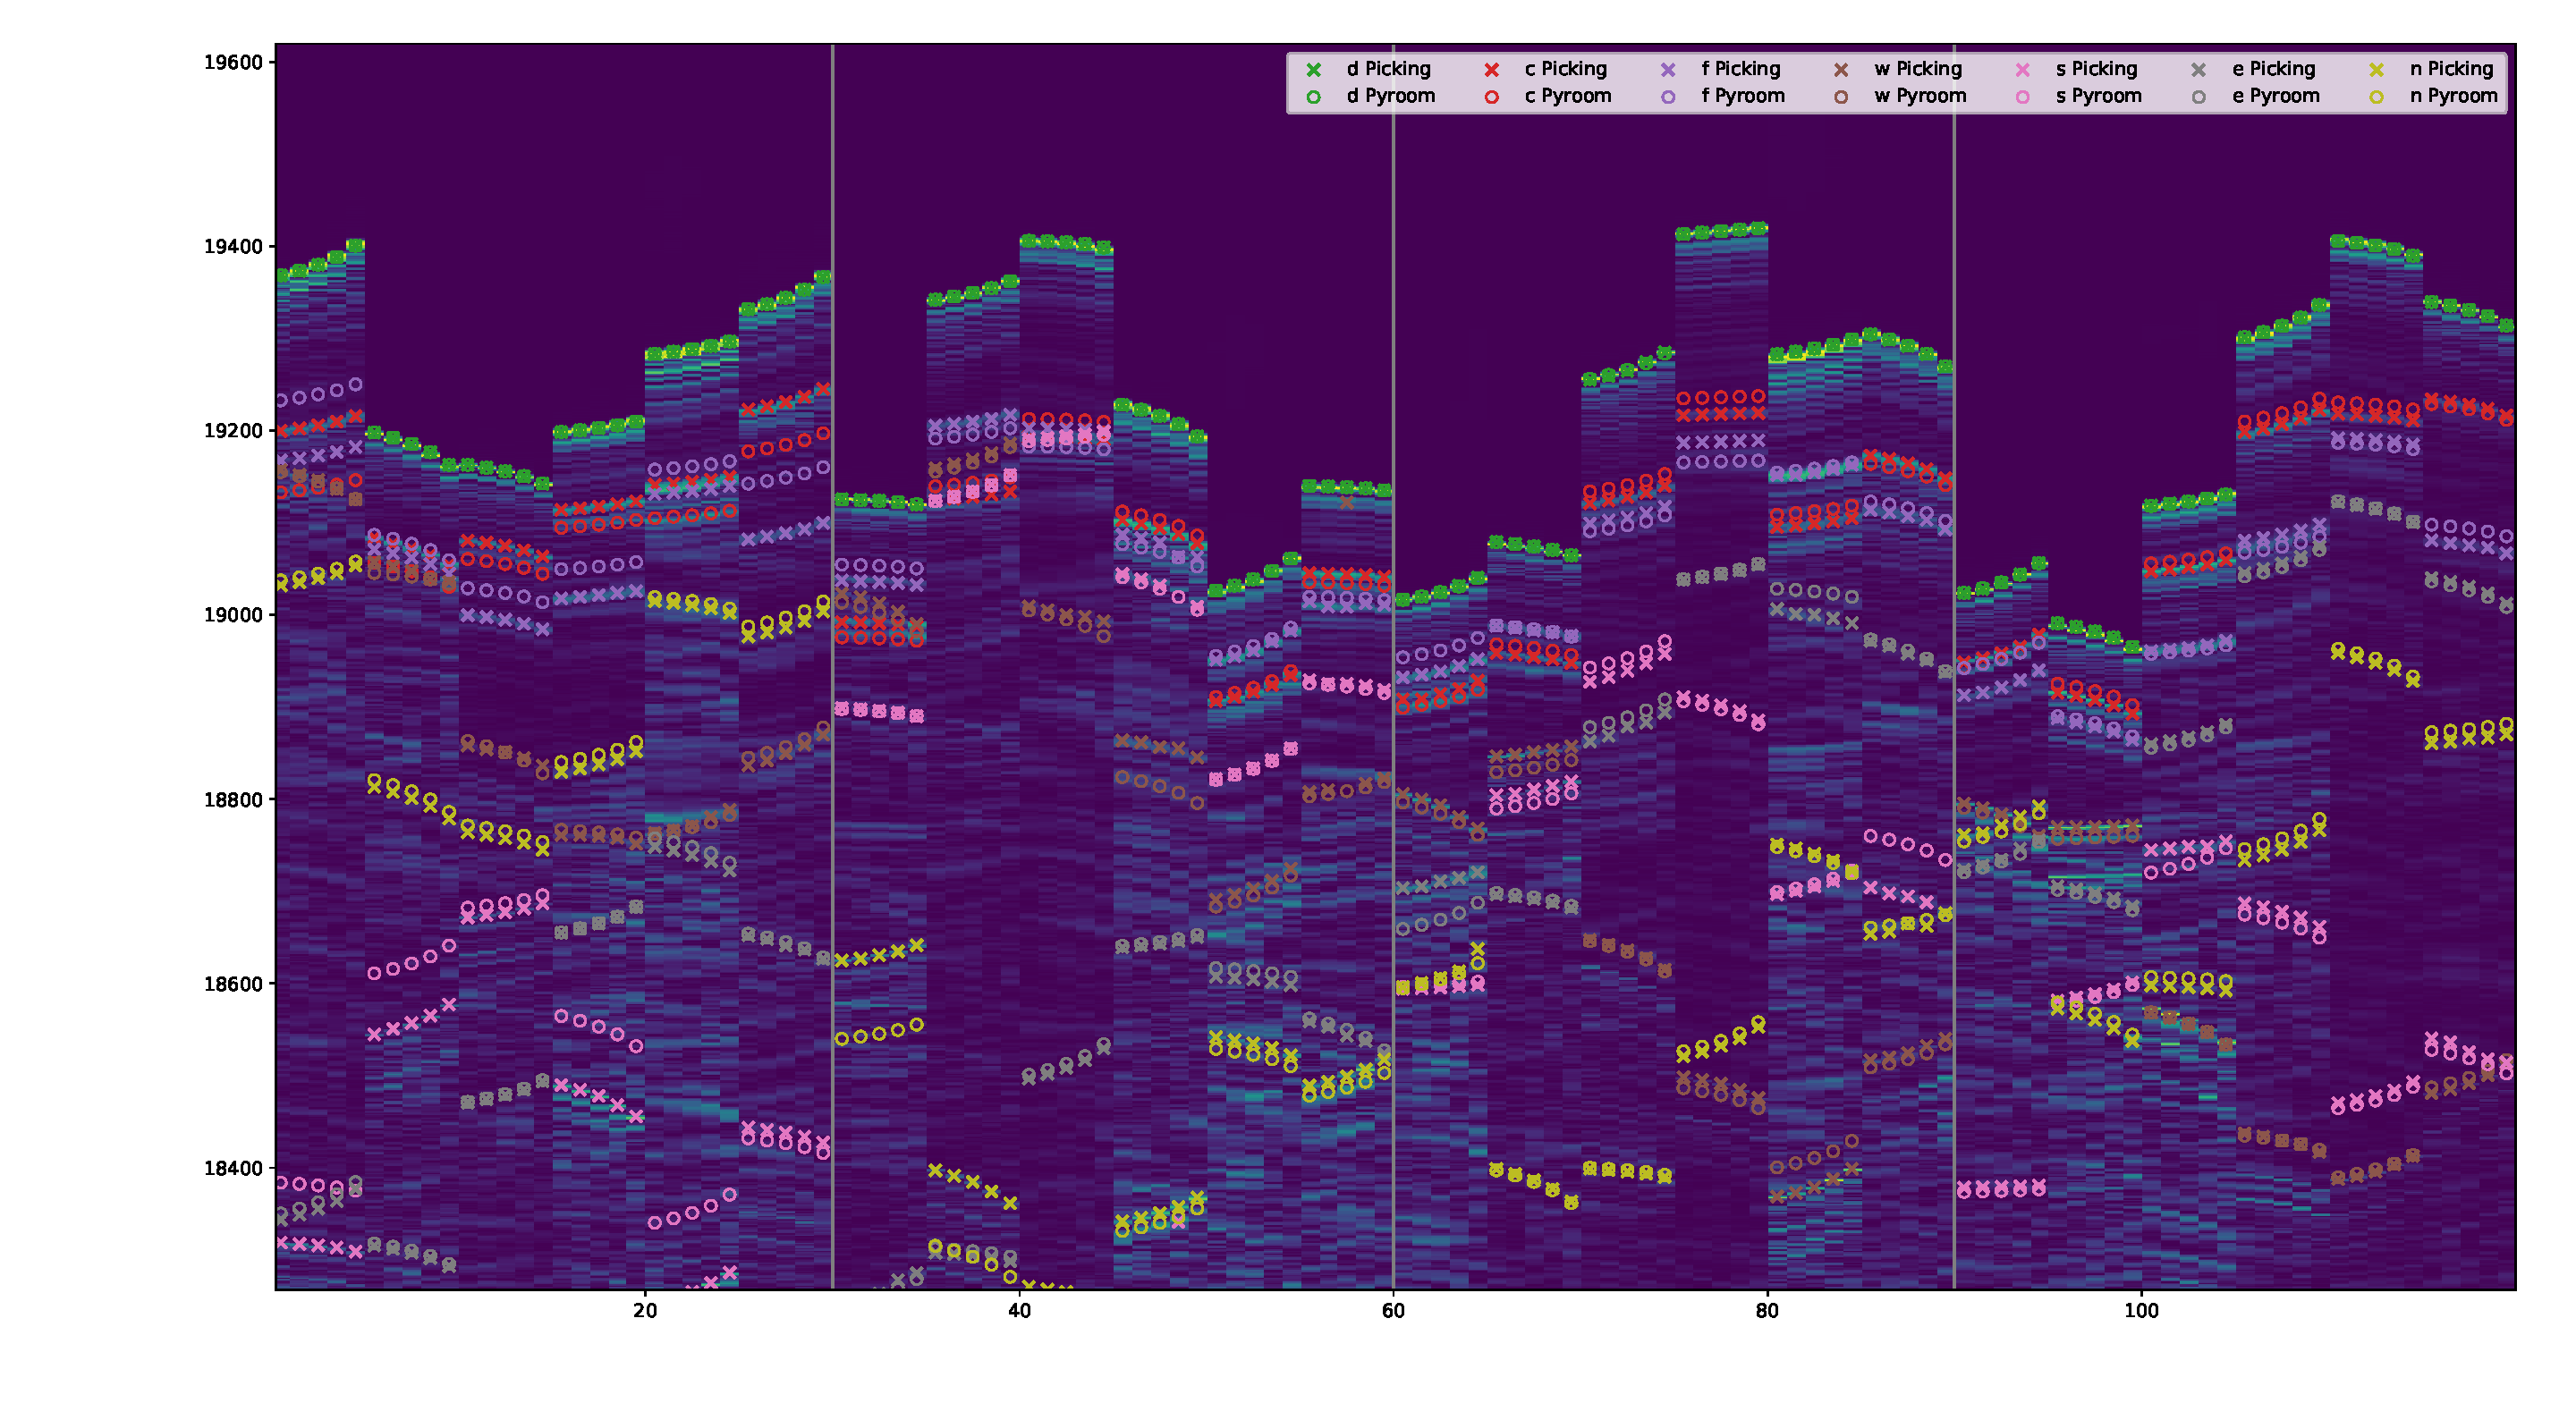
\includegraphics[trim={15em 15em 2em 0},clip,width=\linewidth]{figures/dechorate/rir_skyline_final_mod4paper.pdf}
    \end{sidecaption}
\end{figure}

\newthought{Direct path deconvolution/equalization} was used to compensate the frequency response of the source loudspeaker and microphone \citeonly{antonacci2012inference, Eaton2016estimation}.
In particular, the direct path of the RIR was manually isolated and used as an equalization filter to enhance early reflections from their superimposition and from background noise before proceed with peak picking.
Each \ac{RIR} was equalized with its relative direct path.
As depicted in Figure~\ref{fig:dechorate:labelling_tools}, in some situation this process was necessary for correctly identifying the underlying \TOAs/' peaks.

\newthought{Different wall configurations} for the same geometry influenced the peaks' predominance in the \ac{RIR}, hence facilitating its echo annotation.
An example of \acp{RIR} corresponding to 2 different surface configurations is shown in~\cref{fig:dechorate:labelling_tools}: the reader can notice how the peak predominance changes for the different configurations.

\newthought{An interpolation-based peak finder}\sidenote{
    In this work, peaks are found using the Python \href{https://bitbucket.org/lucashnegri/peakutils/}{\library{peakutils}\ExternalLink} library.
} was used on equalized echograms $\bar{\eta}_{n}(l)$ to provide an initial guess on the peak positions.

\subsection{Limitations of current annotation}
As stated in \citeonly{defrance2008finding}, we want to emphasize that annotating the correct \TOAs/ of echoes and even the direct path in ``clean'' real \acp{RIR} is far from straightforward.
The peaks can be blurred out by the loudspeaker characteristics or the concurrency of multiple reflections.
However as showed in~\cref{fig:dechorate:skyline}, the proposed annotation was found to be sufficiently consistent both in the geometric and in the echo space.
Thus, no further refinement was done.
This database can be used as a first basis to develop better \AER/ methods which could be used to iteratively improve the annotation, for instance including  2$^\text{nd}$ order reflections.

\section{The \library{dEchorate} package}
The dataset comes with both data and code to parse and process it.
The data are presented in 2 modalities: the \texttt{raw} data, that is, the collection of recorded wave files, are organized in folders and can be retrieved by querying a simple database table; the \texttt{processed} data, which comprise the estimated \acp{RIR} and the geometrical and signal annotations, are organized in tensors directly importable in Matlab or Python (\textit{e.g.} all the \acp{RIR} are stored in a tensor of dimension $L \times I \times J \times D$, respectively corresponding to the RIR length in samples, the number of microphones, of sources and of room configurations).
\\Together with the data a Python package is available on the same website.
This includes wrappers, GUI, examples as well as the code to reproduce this study.
In particular, all the scripts used for estimating the \acp{RIR} and annotating them are available and can be used to further improve and enrich the annotation or as baselines for future works.

\begin{figure}
    \begin{sidecaption}[]{
            Sample view of the database table to retrieve the raw wave file and its attributes.
        }[fig:dechorate:dataset]
        \centering
        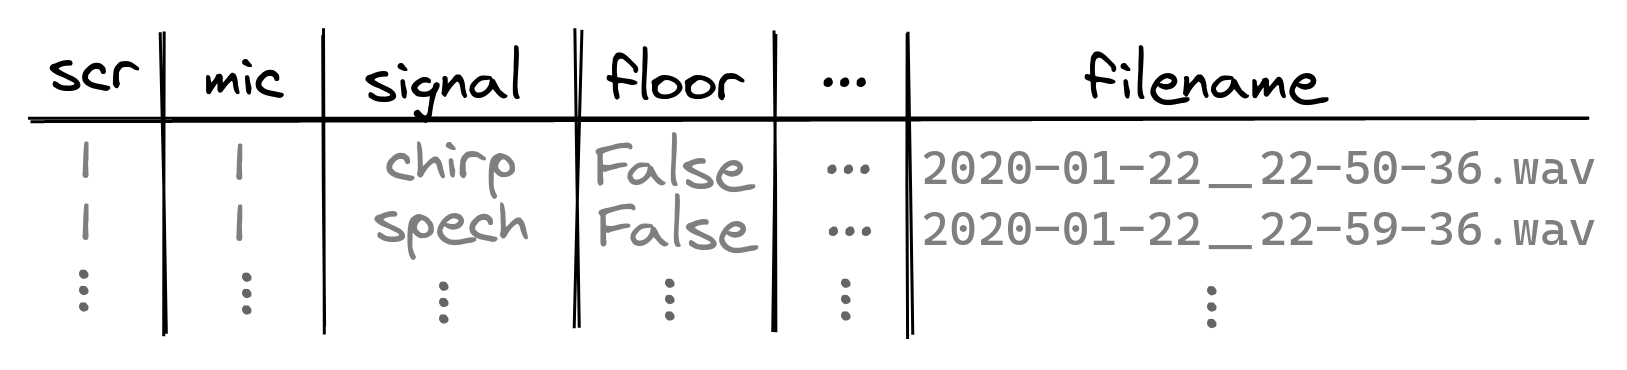
\includegraphics[width=\linewidth]{figures/dechorate/database.png}
    \end{sidecaption}
\end{figure}

\conclusion{This work} introduced a new database of \RIRdef/ featuring accurate annotation of early echoes and microphone positions.
These data can be used to test methods in the room geometry estimation pipeline and in echo-aware audio signal processing.
We will show some application in \SE/ and \RooGE/ in~\cref{ch:dechorateapp}.
\\Future works will explore different directions. By such as making this dataset freely available to the audio signal processing community, we hope to foster research in AER and echo-aware to improve the performance of existing methods on real data.
Moreover, the dataset could be updated by including more robust annotations derived from more advanced algorithms for calibration and \AER/.
\qed

% %% III. Application
% \begin{fullwidth}
%     \part{Echo-aware Application}\label{pt:application}
% \end{fullwidth}
% \parttoc[n]
\chapter{Audio Scene Analysis meets Signal Processing}\label{ch:application}

\newthought{Synopsis} \synopsisChApplication

\mynewline
Here, we present some audio scene analysis problems that will be later discussed in their echo-aware extension.
Following the last part's structure, this introductory chapter gathers the common knowledge shared across the following ones.
Here we make a strong transition: we assume the echo properties are known a priori, so that the our focus is on the benefit of their knowledge.
The literature for each of them is reviewed, but since it is vast and spans diverse scientific research decades, we do not aim to cover it entirely.
Moreover, since the following chapters are dedicated to each of these problems under the echo-aware perspective, this specific literature is not considered here.
\\The material presented here results from the personal synthesis of concepts and references available in the literature.
Furthermore, some definitions are digested from classical textbooks already used for this thesis, such as~\citeonly{vincent2018audio}.

\section{Audio Scene Analysis Problems}\label{sec:application:scenario}
As mentioned in the first chapter, audio scene analysis aims to extract relevant information in the audio scene.
Different types of information are estimated or inferred by solving specific problems.
Despite their diversity, most of these problems can be defined with a common model.

\subsection{Common scenario and model}
Let there be a meeting room with well-defined geometry.
In it, $\numSrcs$ sound sources are located at determined positions, such as some speakers chatting while standing in the room, as in~\cref{fig:estimation:audioscene}.
As an indoor scenario, all the elements of reverberation (in particular echoes) are present.
Diffuse background noise is present as well, for instance, due to the air conditioner or car traffic outside.
This whole audio scene is recorded by a device featuring a microphone array of $\numMics$ sensors.
Furthermore we assume a static far field scenario and we model each $\idxSrc$ sources and $\idxMic$ microphone as well-defined points with coordinate $\positionSource$ and $\positionMicrophone$, respectively.
This is a reasonable assumption in the context of table-top devices, such as smart home devices.
\begin{figure}[]
    \begin{sidecaption}[Audio Scene]{%
        Illustration of an indoor audio scene recorded by three microphones.
        The microphone signals capture the reverberant mixture of several sound sources such as speech, music (guitar) and background diffuse noise (an air conditioner).
    }[fig:estimation:audioscene]
    \centering
    \resizebox{\linewidth}{!}{

\tikzset{every picture/.style={line width=0.75pt}} %set default line width to 0.75pt

\begin{tikzpicture}[x=0.75pt,y=0.75pt,yscale=-1,xscale=1]
%uncomment if require: \path (0,300); %set diagram left start at 0, and has height of 300

%Shape: Circle [id:dp37372160479593475]
\draw  [color={rgb, 255:red, 155; green, 155; blue, 155 }  ,draw opacity=0.76 ][line width=4.5]  (160,196) .. controls (160,184.95) and (168.95,176) .. (180,176) .. controls (191.05,176) and (200,184.95) .. (200,196) .. controls (200,207.05) and (191.05,216) .. (180,216) .. controls (168.95,216) and (160,207.05) .. (160,196) -- cycle ;
%Shape: Circle [id:dp6742469135937114]
\draw  [color={rgb, 255:red, 155; green, 155; blue, 155 }  ,draw opacity=0.76 ][line width=4.5]  (150,196) .. controls (150,179.43) and (163.43,166) .. (180,166) .. controls (196.57,166) and (210,179.43) .. (210,196) .. controls (210,212.57) and (196.57,226) .. (180,226) .. controls (163.43,226) and (150,212.57) .. (150,196) -- cycle ;
%Shape: Circle [id:dp6304501410818584]
\draw   (160,196) .. controls (160,184.95) and (168.95,176) .. (180,176) .. controls (191.05,176) and (200,184.95) .. (200,196) .. controls (200,207.05) and (191.05,216) .. (180,216) .. controls (168.95,216) and (160,207.05) .. (160,196) -- cycle ;
%Shape: Circle [id:dp6073489332662667]
\draw   (150,196) .. controls (150,179.43) and (163.43,166) .. (180,166) .. controls (196.57,166) and (210,179.43) .. (210,196) .. controls (210,212.57) and (196.57,226) .. (180,226) .. controls (163.43,226) and (150,212.57) .. (150,196) -- cycle ;
%Shape: Rectangle [id:dp5920548385374533]
\draw  [draw opacity=0][fill={rgb, 255:red, 255; green, 255; blue, 255 }  ,fill opacity=1 ] (130,230) -- (210,230) -- (210,250) -- (130,250) -- cycle ;
%Image [id:dp7339517530204356]
\draw (480,120) node  {
\includegraphics[width=10pt]{figures/acoustics/iconfinder_microphone_1608550.pdf}};
%Image [id:dp7608229391866312]
\draw (480,80) node  {
\includegraphics[width=10pt]{figures/acoustics/iconfinder_microphone_1608550.pdf}};
%Image [id:dp9664249278995992]
\draw (480,160) node  {\includegraphics[width=10pt]{figures/acoustics/iconfinder_microphone_1608550.pdf}};
%Straight Lines [id:da6875965508418059]
\draw [color={rgb, 255:red, 245; green, 166; blue, 35 }  ,draw opacity=1 ]   (180,120) -- (467.03,80.41) ;
\draw [shift={(470,80)}, rotate = 532.15] [fill={rgb, 255:red, 245; green, 166; blue, 35 }  ,fill opacity=1 ][line width=0.08]  [draw opacity=0] (5.36,-2.57) -- (0,0) -- (5.36,2.57) -- cycle    ;
%Straight Lines [id:da21480429926103284]
\draw [color={rgb, 255:red, 245; green, 166; blue, 35 }  ,draw opacity=1 ]   (180,120) -- (467,120) ;
\draw [shift={(470,120)}, rotate = 180] [fill={rgb, 255:red, 245; green, 166; blue, 35 }  ,fill opacity=1 ][line width=0.08]  [draw opacity=0] (5.36,-2.57) -- (0,0) -- (5.36,2.57) -- cycle    ;
%Straight Lines [id:da6245847985271135]
\draw [color={rgb, 255:red, 245; green, 166; blue, 35 }  ,draw opacity=1 ]   (180,120) -- (467.03,159.59) ;
\draw [shift={(470,160)}, rotate = 187.85] [fill={rgb, 255:red, 245; green, 166; blue, 35 }  ,fill opacity=1 ][line width=0.08]  [draw opacity=0] (5.36,-2.57) -- (0,0) -- (5.36,2.57) -- cycle    ;
%Straight Lines [id:da7309183869115244]
\draw [color={rgb, 255:red, 0; green, 0; blue, 0 }  ,draw opacity=0.2 ] [dash pattern={on 4.5pt off 4.5pt}]  (220,80) -- (310,50) -- (467.05,79.45) ;
\draw [shift={(470,80)}, rotate = 190.62] [fill={rgb, 255:red, 0; green, 0; blue, 0 }  ,fill opacity=0.2 ][line width=0.08]  [draw opacity=0] (5.36,-2.57) -- (0,0) -- (5.36,2.57) -- cycle    ;
%Shape: Rectangle [id:dp15733721403583467]
\draw   (100,50) -- (560,50) -- (560,230) -- (100,230) -- cycle ;
%Straight Lines [id:da2249329781545223]
\draw [color={rgb, 255:red, 0; green, 0; blue, 0 }  ,draw opacity=0.6 ] [dash pattern={on 0.75pt off 0.75pt}]  (212.39,171.35) .. controls (213.1,169.1) and (214.58,168.33) .. (216.83,169.04) .. controls (219.08,169.75) and (220.55,168.98) .. (221.26,166.73) .. controls (221.97,164.48) and (223.44,163.71) .. (225.69,164.42) .. controls (227.94,165.13) and (229.42,164.36) .. (230.13,162.11) .. controls (230.84,159.86) and (232.31,159.09) .. (234.56,159.8) .. controls (236.81,160.5) and (238.28,159.73) .. (238.99,157.48) .. controls (239.7,155.23) and (241.18,154.46) .. (243.43,155.17) .. controls (245.68,155.88) and (247.15,155.11) .. (247.86,152.86) -- (249.44,152.04) -- (256.53,148.34) ;
\draw [shift={(259.19,146.95)}, rotate = 512.46] [fill={rgb, 255:red, 0; green, 0; blue, 0 }  ,fill opacity=0.6 ][line width=0.08]  [draw opacity=0] (5.36,-2.57) -- (0,0) -- (5.36,2.57) -- cycle    ;
%Straight Lines [id:da46872311549917245]
\draw [color={rgb, 255:red, 0; green, 0; blue, 0 }  ,draw opacity=0.6 ] [dash pattern={on 0.75pt off 0.75pt}]  (218.39,184.95) .. controls (219.88,183.12) and (221.54,182.95) .. (223.37,184.44) .. controls (225.2,185.93) and (226.86,185.75) .. (228.34,183.92) .. controls (229.82,182.09) and (231.48,181.91) .. (233.31,183.4) .. controls (235.14,184.89) and (236.8,184.71) .. (238.29,182.88) .. controls (239.78,181.05) and (241.43,180.88) .. (243.26,182.37) .. controls (245.09,183.86) and (246.75,183.68) .. (248.23,181.85) .. controls (249.72,180.02) and (251.38,179.84) .. (253.21,181.33) -- (257.45,180.89) -- (265.41,180.06) ;
\draw [shift={(268.39,179.75)}, rotate = 534.06] [fill={rgb, 255:red, 0; green, 0; blue, 0 }  ,fill opacity=0.6 ][line width=0.08]  [draw opacity=0] (5.36,-2.57) -- (0,0) -- (5.36,2.57) -- cycle    ;
%Straight Lines [id:da41740100207513164]
\draw [color={rgb, 255:red, 0; green, 0; blue, 0 }  ,draw opacity=0.6 ] [dash pattern={on 0.75pt off 0.75pt}]  (213.99,175.35) .. controls (214.96,173.2) and (216.52,172.61) .. (218.67,173.57) .. controls (220.82,174.54) and (222.38,173.94) .. (223.34,171.79) .. controls (224.3,169.64) and (225.86,169.04) .. (228.01,170.01) .. controls (230.16,170.98) and (231.72,170.38) .. (232.68,168.23) .. controls (233.65,166.08) and (235.21,165.48) .. (237.36,166.45) .. controls (239.51,167.42) and (241.07,166.82) .. (242.03,164.67) .. controls (242.99,162.52) and (244.55,161.92) .. (246.7,162.89) .. controls (248.85,163.86) and (250.41,163.26) .. (251.37,161.11) -- (254.11,160.07) -- (261.59,157.22) ;
\draw [shift={(264.39,156.15)}, rotate = 519.15] [fill={rgb, 255:red, 0; green, 0; blue, 0 }  ,fill opacity=0.6 ][line width=0.08]  [draw opacity=0] (5.36,-2.57) -- (0,0) -- (5.36,2.57) -- cycle    ;
%Straight Lines [id:da11925314169744539]
\draw [color={rgb, 255:red, 0; green, 0; blue, 0 }  ,draw opacity=0.6 ] [dash pattern={on 0.75pt off 0.75pt}]  (215.99,180.15) .. controls (217.24,178.16) and (218.87,177.78) .. (220.87,179.03) .. controls (222.87,180.28) and (224.49,179.91) .. (225.74,177.91) .. controls (226.99,175.91) and (228.61,175.54) .. (230.61,176.79) .. controls (232.61,178.04) and (234.23,177.67) .. (235.48,175.67) .. controls (236.73,173.67) and (238.36,173.3) .. (240.36,174.55) .. controls (242.36,175.8) and (243.98,175.42) .. (245.23,173.42) .. controls (246.48,171.42) and (248.1,171.05) .. (250.1,172.3) .. controls (252.1,173.55) and (253.72,173.18) .. (254.97,171.18) -- (255.67,171.02) -- (263.47,169.23) ;
\draw [shift={(266.39,168.55)}, rotate = 527.04] [fill={rgb, 255:red, 0; green, 0; blue, 0 }  ,fill opacity=0.6 ][line width=0.08]  [draw opacity=0] (5.36,-2.57) -- (0,0) -- (5.36,2.57) -- cycle    ;
%Straight Lines [id:da12240342341771249]
\draw [color={rgb, 255:red, 208; green, 2; blue, 27 }  ,draw opacity=1 ] [dash pattern={on 0.75pt off 0.75pt}]  (510,150) .. controls (509.26,152.24) and (507.77,152.99) .. (505.53,152.24) .. controls (503.3,151.49) and (501.81,152.24) .. (501.06,154.47) -- (499.84,155.08) -- (492.68,158.66) ;
\draw [shift={(490,160)}, rotate = 333.43] [fill={rgb, 255:red, 208; green, 2; blue, 27 }  ,fill opacity=1 ][line width=0.08]  [draw opacity=0] (5.36,-2.57) -- (0,0) -- (5.36,2.57) -- cycle    ;
%Straight Lines [id:da5418102098206483]
\draw [color={rgb, 255:red, 208; green, 2; blue, 27 }  ,draw opacity=1 ] [dash pattern={on 0.75pt off 0.75pt}]  (510,110) .. controls (509.26,112.24) and (507.77,112.99) .. (505.53,112.24) .. controls (503.3,111.49) and (501.81,112.24) .. (501.06,114.47) -- (499.84,115.08) -- (492.68,118.66) ;
\draw [shift={(490,120)}, rotate = 333.43] [fill={rgb, 255:red, 208; green, 2; blue, 27 }  ,fill opacity=1 ][line width=0.08]  [draw opacity=0] (5.36,-2.57) -- (0,0) -- (5.36,2.57) -- cycle    ;
%Straight Lines [id:da2263274179236877]
\draw [color={rgb, 255:red, 208; green, 2; blue, 27 }  ,draw opacity=1 ] [dash pattern={on 0.75pt off 0.75pt}]  (510,60) .. controls (509.26,62.24) and (507.77,62.99) .. (505.53,62.24) .. controls (503.3,61.49) and (501.81,62.24) .. (501.06,64.47) -- (499.84,65.08) -- (492.68,68.66) ;
\draw [shift={(490,70)}, rotate = 333.43] [fill={rgb, 255:red, 208; green, 2; blue, 27 }  ,fill opacity=1 ][line width=0.08]  [draw opacity=0] (5.36,-2.57) -- (0,0) -- (5.36,2.57) -- cycle    ;
%Straight Lines [id:da6407483239165986]
\draw [color={rgb, 255:red, 0; green, 0; blue, 0 }  ,draw opacity=0.2 ] [dash pattern={on 4.5pt off 4.5pt}]  (220,80) -- (350,230) -- (468.13,82.34) ;
\draw [shift={(470,80)}, rotate = 488.66] [fill={rgb, 255:red, 0; green, 0; blue, 0 }  ,fill opacity=0.2 ][line width=0.08]  [draw opacity=0] (5.36,-2.57) -- (0,0) -- (5.36,2.57) -- cycle    ;
%Straight Lines [id:da5328192505993826]
\draw [color={rgb, 255:red, 0; green, 0; blue, 0 }  ,draw opacity=0.2 ] [dash pattern={on 4.5pt off 4.5pt}]  (220,80) -- (330,50) -- (467.32,118.66) ;
\draw [shift={(470,120)}, rotate = 206.57] [fill={rgb, 255:red, 0; green, 0; blue, 0 }  ,fill opacity=0.2 ][line width=0.08]  [draw opacity=0] (5.36,-2.57) -- (0,0) -- (5.36,2.57) -- cycle    ;
%Straight Lines [id:da8377831024194228]
\draw [color={rgb, 255:red, 0; green, 0; blue, 0 }  ,draw opacity=0.2 ] [dash pattern={on 4.5pt off 4.5pt}]  (220,80) -- (370,230) -- (468.34,82.5) ;
\draw [shift={(470,80)}, rotate = 483.69] [fill={rgb, 255:red, 0; green, 0; blue, 0 }  ,fill opacity=0.2 ][line width=0.08]  [draw opacity=0] (5.36,-2.57) -- (0,0) -- (5.36,2.57) -- cycle    ;
%Straight Lines [id:da38697516677735044]
\draw [color={rgb, 255:red, 0; green, 0; blue, 0 }  ,draw opacity=0.2 ] [dash pattern={on 4.5pt off 4.5pt}]  (220,80) -- (400,230) -- (467.88,162.12) ;
\draw [shift={(470,160)}, rotate = 495] [fill={rgb, 255:red, 0; green, 0; blue, 0 }  ,fill opacity=0.2 ][line width=0.08]  [draw opacity=0] (5.36,-2.57) -- (0,0) -- (5.36,2.57) -- cycle    ;
%Image [id:dp4512377721787463]
\draw (200,80) node  {\includegraphics[width=30pt]{figures/speech.pdf}};
%Image [id:dp11655856762581418]
\draw (160,120) node  {\includegraphics[width=45pt]{figures/guitar.pdf}};
%Straight Lines [id:da6506133051173556]
\draw [color={rgb, 255:red, 0; green, 0; blue, 0 }  ,draw opacity=0.6 ] [dash pattern={on 0.75pt off 0.75pt}]  (218.06,191.95) .. controls (219.65,190.21) and (221.31,190.13) .. (223.05,191.72) .. controls (224.8,193.31) and (226.46,193.23) .. (228.05,191.48) .. controls (229.64,189.74) and (231.3,189.66) .. (233.04,191.25) .. controls (234.78,192.84) and (236.45,192.76) .. (238.04,191.02) .. controls (239.62,189.27) and (241.28,189.19) .. (243.03,190.78) .. controls (244.77,192.37) and (246.44,192.29) .. (248.03,190.55) .. controls (249.61,188.8) and (251.27,188.72) .. (253.02,190.31) -- (257.45,190.1) -- (265.44,189.73) ;
\draw [shift={(268.43,189.59)}, rotate = 537.31] [fill={rgb, 255:red, 0; green, 0; blue, 0 }  ,fill opacity=0.6 ][line width=0.08]  [draw opacity=0] (5.36,-2.57) -- (0,0) -- (5.36,2.57) -- cycle    ;
%Straight Lines [id:da9912250072749541]
\draw [color={rgb, 255:red, 245; green, 166; blue, 35 }  ,draw opacity=0.3 ] [dash pattern={on 4.5pt off 4.5pt}]  (180,120) -- (290,230) -- (467.7,81.92) ;
\draw [shift={(470,80)}, rotate = 500.19] [fill={rgb, 255:red, 245; green, 166; blue, 35 }  ,fill opacity=0.3 ][line width=0.08]  [draw opacity=0] (5.36,-2.57) -- (0,0) -- (5.36,2.57) -- cycle    ;
%Straight Lines [id:da842755271595558]
\draw [color={rgb, 255:red, 245; green, 166; blue, 35 }  ,draw opacity=0.3 ] [dash pattern={on 4.5pt off 4.5pt}]  (180,120) -- (310,230) -- (467.53,121.7) ;
\draw [shift={(470,120)}, rotate = 505.49] [fill={rgb, 255:red, 245; green, 166; blue, 35 }  ,fill opacity=0.3 ][line width=0.08]  [draw opacity=0] (5.36,-2.57) -- (0,0) -- (5.36,2.57) -- cycle    ;
%Straight Lines [id:da565897385867932]
\draw [color={rgb, 255:red, 245; green, 166; blue, 35 }  ,draw opacity=0.3 ] [dash pattern={on 4.5pt off 4.5pt}]  (180,120) -- (340,230) -- (467.36,161.42) ;
\draw [shift={(470,160)}, rotate = 511.7] [fill={rgb, 255:red, 245; green, 166; blue, 35 }  ,fill opacity=0.3 ][line width=0.08]  [draw opacity=0] (5.36,-2.57) -- (0,0) -- (5.36,2.57) -- cycle    ;
%Straight Lines [id:da016277657003535784]
\draw [color={rgb, 255:red, 0; green, 0; blue, 0 }  ,draw opacity=0.6 ] [dash pattern={on 0.75pt off 0.75pt}]  (215.77,214.66) .. controls (218.07,214.14) and (219.48,215.03) .. (219.99,217.33) .. controls (220.51,219.63) and (221.92,220.52) .. (224.22,220.01) .. controls (226.52,219.49) and (227.93,220.38) .. (228.44,222.68) .. controls (228.95,224.98) and (230.36,225.87) .. (232.66,225.35) .. controls (234.96,224.84) and (236.37,225.73) .. (236.89,228.03) -- (240,230) -- (240,230) .. controls (240.17,227.65) and (241.44,226.56) .. (243.79,226.74) .. controls (246.14,226.92) and (247.41,225.83) .. (247.58,223.48) .. controls (247.76,221.13) and (249.03,220.04) .. (251.38,220.22) .. controls (253.73,220.4) and (255,219.31) .. (255.17,216.96) .. controls (255.34,214.61) and (256.61,213.52) .. (258.96,213.7) -- (260.76,212.16) -- (266.82,206.94) ;
\draw [shift={(269.1,204.99)}, rotate = 499.32] [fill={rgb, 255:red, 0; green, 0; blue, 0 }  ,fill opacity=0.6 ][line width=0.08]  [draw opacity=0] (5.36,-2.57) -- (0,0) -- (5.36,2.57) -- cycle    ;
%Straight Lines [id:da9867855512078149]
\draw [color={rgb, 255:red, 0; green, 0; blue, 0 }  ,draw opacity=0.6 ] [dash pattern={on 0.75pt off 0.75pt}]  (218.1,207.99) .. controls (220.42,207.56) and (221.79,208.51) .. (222.22,210.83) .. controls (222.64,213.15) and (224.01,214.1) .. (226.33,213.67) .. controls (228.65,213.24) and (230.02,214.19) .. (230.45,216.51) .. controls (230.87,218.83) and (232.24,219.78) .. (234.56,219.35) .. controls (236.88,218.92) and (238.25,219.87) .. (238.68,222.19) .. controls (239.1,224.51) and (240.47,225.46) .. (242.79,225.03) .. controls (245.11,224.6) and (246.48,225.55) .. (246.91,227.87) -- (250,230) -- (250,230) .. controls (250.29,227.66) and (251.6,226.63) .. (253.94,226.92) .. controls (256.28,227.21) and (257.59,226.18) .. (257.88,223.84) .. controls (258.17,221.5) and (259.48,220.48) .. (261.82,220.77) .. controls (264.16,221.06) and (265.47,220.03) .. (265.76,217.69) -- (266.1,217.43) -- (272.4,212.5) ;
\draw [shift={(274.77,210.66)}, rotate = 502.01] [fill={rgb, 255:red, 0; green, 0; blue, 0 }  ,fill opacity=0.6 ][line width=0.08]  [draw opacity=0] (5.36,-2.57) -- (0,0) -- (5.36,2.57) -- cycle    ;
%Straight Lines [id:da5055644084768178]
\draw [color={rgb, 255:red, 0; green, 0; blue, 0 }  ,draw opacity=0.6 ] [dash pattern={on 0.75pt off 0.75pt}]  (210,220.33) .. controls (212.23,219.59) and (213.72,220.34) .. (214.47,222.57) .. controls (215.21,224.81) and (216.7,225.56) .. (218.94,224.81) .. controls (221.17,224.06) and (222.67,224.81) .. (223.42,227.04) .. controls (224.16,229.28) and (225.65,230.03) .. (227.89,229.28) -- (230,230.33) -- (230,230.33) .. controls (230.17,227.98) and (231.44,226.9) .. (233.79,227.07) .. controls (236.14,227.25) and (237.41,226.16) .. (237.58,223.81) .. controls (237.75,221.46) and (239.02,220.37) .. (241.37,220.55) .. controls (243.72,220.73) and (244.99,219.64) .. (245.16,217.29) .. controls (245.33,214.94) and (246.6,213.85) .. (248.95,214.03) .. controls (251.3,214.21) and (252.57,213.12) .. (252.74,210.77) -- (255.76,208.16) -- (261.83,202.95) ;
\draw [shift={(264.1,200.99)}, rotate = 499.29] [fill={rgb, 255:red, 0; green, 0; blue, 0 }  ,fill opacity=0.6 ][line width=0.08]  [draw opacity=0] (5.36,-2.57) -- (0,0) -- (5.36,2.57) -- cycle    ;
%Straight Lines [id:da5832987622194876]
\draw [color={rgb, 255:red, 0; green, 0; blue, 0 }  ,draw opacity=0.2 ] [dash pattern={on 4.5pt off 4.5pt}]  (220,80) -- (350,50) -- (467.79,157.97) ;
\draw [shift={(470,160)}, rotate = 222.51] [fill={rgb, 255:red, 0; green, 0; blue, 0 }  ,fill opacity=0.2 ][line width=0.08]  [draw opacity=0] (5.36,-2.57) -- (0,0) -- (5.36,2.57) -- cycle    ;
%Straight Lines [id:da5008400993643431]
\draw [color={rgb, 255:red, 245; green, 166; blue, 35 }  ,draw opacity=0.3 ] [dash pattern={on 4.5pt off 4.5pt}]  (180,120) -- (350,50) -- (467.79,157.97) ;
\draw [shift={(470,160)}, rotate = 222.51] [fill={rgb, 255:red, 245; green, 166; blue, 35 }  ,fill opacity=0.3 ][line width=0.08]  [draw opacity=0] (5.36,-2.57) -- (0,0) -- (5.36,2.57) -- cycle    ;
%Straight Lines [id:da2480092091139493]
\draw [color={rgb, 255:red, 245; green, 166; blue, 35 }  ,draw opacity=0.3 ] [dash pattern={on 4.5pt off 4.5pt}]  (180,120) -- (370,50) -- (467.54,118.28) ;
\draw [shift={(470,120)}, rotate = 214.99] [fill={rgb, 255:red, 245; green, 166; blue, 35 }  ,fill opacity=0.3 ][line width=0.08]  [draw opacity=0] (5.36,-2.57) -- (0,0) -- (5.36,2.57) -- cycle    ;
%Straight Lines [id:da98913951227942]
\draw [color={rgb, 255:red, 245; green, 166; blue, 35 }  ,draw opacity=0.3 ] [dash pattern={on 4.5pt off 4.5pt}]  (180,120) -- (400,50) -- (467.24,78.82) ;
\draw [shift={(470,80)}, rotate = 203.2] [fill={rgb, 255:red, 245; green, 166; blue, 35 }  ,fill opacity=0.3 ][line width=0.08]  [draw opacity=0] (5.36,-2.57) -- (0,0) -- (5.36,2.57) -- cycle    ;
%Straight Lines [id:da7940761686938484]
\draw [color={rgb, 255:red, 74; green, 74; blue, 74 }  ,draw opacity=1 ]   (220,80) -- (467,80) ;
\draw [shift={(470,80)}, rotate = 180] [fill={rgb, 255:red, 74; green, 74; blue, 74 }  ,fill opacity=1 ][line width=0.08]  [draw opacity=0] (5.36,-2.57) -- (0,0) -- (5.36,2.57) -- cycle    ;
%Straight Lines [id:da03582329188397548]
\draw [color={rgb, 255:red, 74; green, 74; blue, 74 }  ,draw opacity=1 ]   (220,80) -- (467.04,119.53) ;
\draw [shift={(470,120)}, rotate = 189.09] [fill={rgb, 255:red, 74; green, 74; blue, 74 }  ,fill opacity=1 ][line width=0.08]  [draw opacity=0] (5.36,-2.57) -- (0,0) -- (5.36,2.57) -- cycle    ;
%Straight Lines [id:da5309831276841109]
\draw [color={rgb, 255:red, 74; green, 74; blue, 74 }  ,draw opacity=1 ]   (220,80) -- (467.14,159.09) ;
\draw [shift={(470,160)}, rotate = 197.74] [fill={rgb, 255:red, 74; green, 74; blue, 74 }  ,fill opacity=1 ][line width=0.08]  [draw opacity=0] (5.36,-2.57) -- (0,0) -- (5.36,2.57) -- cycle    ;
%Image [id:dp7579313396430111]
\draw (180,196) node  {\includegraphics[width=18.75pt]{figures/ac.pdf}};
%Straight Lines [id:da14142044437195245]
\draw    (480,90) -- (577,90) ;
\draw [shift={(580,90)}, rotate = 180] [fill={rgb, 255:red, 0; green, 0; blue, 0 }  ][line width=0.08]  [draw opacity=0] (7.14,-3.43) -- (0,0) -- (7.14,3.43) -- (4.74,0) -- cycle    ;
%Straight Lines [id:da0847611097781068]
\draw    (480,130) -- (577,130) ;
\draw [shift={(580,130)}, rotate = 180] [fill={rgb, 255:red, 0; green, 0; blue, 0 }  ][line width=0.08]  [draw opacity=0] (7.14,-3.43) -- (0,0) -- (7.14,3.43) -- (4.74,0) -- cycle    ;
%Straight Lines [id:da009579756930902739]
\draw    (480,170) -- (577,170) ;
\draw [shift={(580,170)}, rotate = 180] [fill={rgb, 255:red, 0; green, 0; blue, 0 }  ][line width=0.08]  [draw opacity=0] (7.14,-3.43) -- (0,0) -- (7.14,3.43) -- (4.74,0) -- cycle    ;

% Text Node
\draw (467,95.4) node [anchor=north west][inner sep=0.75pt]  [font=\footnotesize]  {$\positionMicrophone_{1}$};
% Text Node
\draw (467,135.4) node [anchor=north west][inner sep=0.75pt]  [font=\footnotesize]  {$\positionMicrophone_{2}$};
% Text Node
\draw (467,175.4) node [anchor=north west][inner sep=0.75pt]  [font=\footnotesize]  {$\positionMicrophone_{3}$};
% Text Node
\draw (577,76.4) node [anchor=north west][inner sep=0.75pt]  [font=\footnotesize]  {$\mic_{1}$};
% Text Node
\draw (577,116.4) node [anchor=north west][inner sep=0.75pt]  [font=\footnotesize]  {$\mic_{2}$};
% Text Node
\draw (577,156.4) node [anchor=north west][inner sep=0.75pt]  [font=\footnotesize]  {$\mic_{3}$};
% Text Node
\draw (221,65.4) node [anchor=north west][inner sep=0.75pt]  [font=\footnotesize]  {$\src_{1}$};
% Text Node
\draw (204,101.4) node [anchor=north west][inner sep=0.75pt]  [font=\footnotesize]  {$\positionSource_{1}$};
% Text Node
\draw (171,117.4) node [anchor=north west][inner sep=0.75pt]  [font=\footnotesize,color={rgb, 255:red, 245; green, 166; blue, 35 }  ,opacity=1 ]  {$\src_{2}$};
% Text Node
\draw (151,149.4) node [anchor=north west][inner sep=0.75pt]  [font=\footnotesize,color={rgb, 255:red, 245; green, 166; blue, 35 }  ,opacity=1 ]  {$\positionSource_{2}$};
% Text Node
\draw (201,160.4) node [anchor=north west][inner sep=0.75pt]  [font=\footnotesize,color={rgb, 255:red, 128; green, 128; blue, 128 }  ,opacity=1 ]  {$\nse$};


\end{tikzpicture}
}
    \end{sidecaption}
\end{figure}
Recalling the (discrete) time-domain signal model already discussed in~\cref{subsec:processing:mixing}, the signal recorded at the $\idxMic$-th microphones reads
\begin{equation}
    \label{eq:application:mix}
    \mic_\idxMic[n] = \sum_{\idxSrc = 1}^{\numSrcs}
        \kparen{\flt_{\idxMicSrc}( \positionMicrophone_{\idxMic}  | \positionSource_{\idxSrc}) \convDis \src_{\idxSrc}} [n] + \nse_\idxMic[n]
    ,
\end{equation}
or alternatively, using the source spatial image signals,
\begin{equation}
    \label{eq:application:mix_img}
    \begin{aligned}
        \img_{\idxMicSrc}[n]  &= \kparen{\flt_{\idxMicSrc}( \positionMicrophone_{\idxMic}  | \positionSource_{\idxSrc}) \convDis \src_{\idxSrc}}[n]
        \mic_\idxMic[n]     &= \sum_{\idxSrc = 1}^{\numSrcs} \img_{\idxMicSrc}[n] + \nse_\idxMic[n],\\
        .
    \end{aligned}
\end{equation}
Note that the filter $\flt_{\idxMicSrc}(\positionMicrophone_{\idxMic} | \positionSource_{\idxSrc})$ denotes the \RIR/ where we intentionally highlight the dependencies on geometry,
namely, accounting for the whole sound propagation for the source position $\positionSource_{\idxSrc}$ to the microphone position $\positionMicrophone_{\idxMic}$.
In fact, as discussed throughout~\cref{pt:background}, we can decouple the information of indoor microphone natural recordings into two orthogonal contributions:
the \RIRs/ (thus the mixing matrix) accounting for only the sound propagation, and the source signals describes only the semantic content.

\newcommand{\setMicSignals}{\ensuremath{\set{\mic_{\idxMic}}_\idxMic}}
\newcommand{\setSrcSignals}{\ensuremath{\set{\src_{\idxSrc}}_\idxSrc}}
\newcommand{\setSrcPositions}{\ensuremath{\set{\positionSource_{\idxSrc}}_\idxSrc}}
\newcommand{\setFltSignals}{\ensuremath{\set{\flt_{\idxMicSrc}(\positionMicrophone_{\idxMic} | \positionSource_{\idxSrc})}_{\idxMicSrc}}}


\subsection{Problem formulation}
The Audio Scene Analysis Problems presented already in the introductory chapter (See~\cref{sec:intro:scene}) can now be extended and rewritten in terms of the above notation.
Furthermore, we will consider here the only ones directly addressed in this thesis: room impulse response estimation, audio source separation, Spatial filtering, sound source localization, and room geometry estimation.

\begin{table}[!h]

    \begin{fullwidth}
    \centering
    \small
    \renewcommand{\arraystretch}{1.3}

    \begin{tabular*}{\linewidth}{@{\extracolsep{\fill}}lllll@{}}
    \toprule
    Audio scene analysis problems & \textit{from the mixtures $\setMicSignals$, can we estimate...}  & Chapter\\
    \midrule

    Audio Source Separation     & \begin{tabular}[c]{@{}l@{}}the source signals $\setSrcSignals$ and\\ \hspace{1em} the filters $\setFltSignals$?\end{tabular}   & \cref{ch:separake}\\

    Spatial filtering           & \begin{tabular}[c]{@{}l@{}}the source signals $\setSrcSignals$,\\ \hspace{1em} knowing the filters $\setFltSignals$?\end{tabular} & \cref{ch:decharateapp}~\cref{sec:dechorateapp:se}\\

    Sound Source Localization   & the source positions $\setSrcPositions$?                              & \cref{ch:mirage}\\

    Room Geometry Estimation    & the shape of the room?                                                & \cref{ch:decharateapp}~\cref{sec:dechorateapp:rooge}\\
    \bottomrule
\end{tabular*}


% Channel (or \RIR/) Estimation            & the filters $\setFltSignals$ ?                            & \cref{pt:estimation}\\

% Acoustic Echo Retrieval     & the early echoes' timings and gain accounted in $\setFltSignals$ ?     & \cref{pt:estimation}\\

% \RIR/ measurement           & the filters $\setFltSignals$, knowing $\setSrcSignals$ ?               & \cref{ch:dechorate}\\
% Speech Enhancement          & the signal of the $\idxSrc$-th target source $\src_{\idxSrc}$?        & \cref{ch:decharateapp}\\

    % \hline

    \caption{List of audio scene analysis problems considered in this thesis accompanied by their mathematical description.}
    \label{tab:application:problems}

    \end{fullwidth}

\end{table}

\mynewline
As introduced in~\cref{sec:estimation:problem}, these problems can be said either \textit{informed} or \textit{blind} and the related scenario \textit{active} or \textit{passive}.
These two dichotomies emphasize the amount of prior knowledge available for solving them.
As opposed to the active scenario, where the source signal is known, transmitted, and available, the passive one considers only the microphone measurements.
For instance, when addressing the active echo estimation problem or \RIR/ measurement, the exact time of emission of the source signal is known, as well as the source signal itself.
\\The second dichotomy refers to the possibility of exploiting prior knowledge to solve the problem more easily.
This information may derive from annotations and meta-data.
In the community of audio source separation, the following definitions were proposed in~\citeonly{vincent2014blind}:
as opposed to informed problems, for solving the blind ones, absolutely no information is given about the source signal or the mixing process.
In between, there are \textit{semi-blind} or \textit{guided} problems:
here general information is available, such as on the nature of the source signal (speech, music, environmental sounds),
microphone position, recording scenario (indoor, outdoor, professional music), mixing process, \etc/.
In some books and works other categories of problems are defined, such as \emph{weakly-guided}, \emph{strongly-guided}.
Here we do not consider these distinctions.

\mynewline
In the considered echo-aware applications, the echoes properties build our prior knowledge on the problem.
Therefore, according to the above taxonomy, the addressed problems are necessarily guided.
In general and unless specified, this is the only knowledge we will assume to have.
Based on this, we will now review some classical works for solving the above problems.


\newthought{In the following sections} we will present the general overview of the literature related to the problems considered in this thesis: multichannel audio source separation, Spatial filtering, and sound source localization.
We will limit the discussion to the most relevant techniques adopted nowadays with respect to the acoustic propagation modeling.
Later in the thesis, dedicated sections on echo-aware method to address these problems will be provided in each related chapter.
Since room geometry estimation is mainly based on echo estimation and labeling discussed in~\cref{subsec:estimation:active_rir}, its description is postponed to~\cref{sec:dechorateapp:rooge}.


\section{Overview on multichannel Sound Source Separation}\label{sec:application:separation}
Multichannel audio source separation refers to the process of extracting acoustic signals from multichannel mixtures featuring targets, interfering, and noisy sounds.
In psychoacoustics, this problem is known as \textit{the cocktail party problem}~\citeonly{cherry1953cocktail}, referring to the human ability to focus on a particular stimulus in a audio scene.
This problem has interested mainly in two research fields in the audio signal processing community: speech and music processing.
Both share many methods, which are accordingly modified, taking into account scenarios and applications.
\marginpar{
    \footnotesize\itshape
    Many other methods have been proposed in the literature.
    The reader can refer to \citeonly{vincent2018audio, makino2018audio}
}
In the context of the multichannel speech recordings, some of the most successful and popular methods used nowadays
include Spatial filtering, \TF/ masking, and end-to-end regression.
In this thesis, we deliberately distinguish between the Spatial filtering, which will be discussed in the following subsection, and \TF/ masking.
\\\TF/ masking relies on \TF/ diversity of the sources and processes each mixture channel separately.
In a nutshell, it involves computing the \acp{STFT} of the mixture channels, multiplying them by masks containing gains between 0 and 1.
One of the most popular masking rules is adaptive Wiener filtering.
For each time-frequency bin, the \acp{STFT} of the estimated source spatial images $\IMG_{\idxMicSrc}$ of the $\idxSrc$-th source at the $\idxMic$ microphone, writes
\begin{equation}
        \hat{\IMG}_{\idxMicSrc} = \underbrace{\frac{\powerOf{\IMG_{\idxMicSrc}}}
                                        {\sum_{\idxSrc=0}^\numSrcs \powerOf{\IMG_{\idxMicSrc}}}}
                                        _{\text{Wiener filter}} \; \MIC_\idxMic
\end{equation}
where $\MIC_\idxMic$ is the \STFT/ of the microphone channel. Here the \TF/ bin is omitted for clarity.
\\In order to be computed, the Wiener filter requires estimating all the source spatial images, or equivalently, the mixing filters and the source signals.
Therefore, this approach has been generalized in several ways to account for both these unknowns.
In these thesis we stress the difference between source separation and Spatial filtering.
In the former, all the source signals and mixing filters are indispensable to weigh each of the \TF/ bins of the microphone channel's \STFT/.
As opposed to, in the latter problem, the ``masks'', that is the spatial filters, are estimate only based the mixing filters and noise statistics.
In multichannel recordings, a clear overlap exist between the two problems, and some techniques can be used reciprocally.
Furthermore the related research trends are now converging under the same umbrella of the so-called \textit{speech enhancement}.
The work~\citeonly{gannot2017consolidated} provide an unified framework merging source separation and Spatial filtering.
Nevertheless, we will treat them as separated problems.

\mynewline
Moreover, the benefit of the \TF/ masking approach is that the masks can be estimated in various ways.
For instance, clustering and classification techniques~\citeonly{rickard2007duet} can be used to assign each \TF/-bin to each of the sources.
Recently learning-based methods have been used in this sense on the same task~\citeonly{hershey2016deep,wang2018multi}.
Alternatively, deep learning techniques can used to directly estimated the sources' \TF/, as done in one of the reference implementation~\citeonly{stoter2019open}.
The work of \citeonly{nugraha2016multichannel}, instead, uses a deep learning model build by unfolding the the popular Multichannel \ac{NMF} source separation framework of~\citeonly{ozerov2010multichannel, sawada2013multichannel}.

\mynewline
The Gaussian-based Multichannel \ac{NMF}~\citeonly{ozerov2010multichannel} is one of the most successful framework for source separation using \TF/ masks.
It combines the \ac{NMF} and narrowband spatial model (discussed in ~\cref{subsec:processing:model:stft}) and deploys optimization-based framework for estimating both the mixing matrix and the sources.
One of the main advantage of this approach is that it allows to easily incorporated prior knowledge on the problem.
Thanks to the narrowband approximation (\cref{eq:processing:narrow}), spatial and semantic content are orthogonal and can be treated disjointedly.
This opens to many possibilities, such as, using pre-trained dictionaries to model source content~\citeonly{schmidt2006single, smaragdis2009sparse}, or using proper model for the mixing filters, such as \RIRs/, steering vectors, \ReTFs/, \etc/.

\mynewline
However, it has been shown that even with oracle \TF/~\citeonly{luo2019conv}, the estimation is still affected by artifacts.
This limitation affects all the approaches operating in the \TF/ domain.
To overcome this, end-to-deep deep learning models~\citeonly{luo2019conv, tzinis2020sudo} were developed and now hold the record in source separation.
These models work directly in the time domain: both input and output are time-domain waveforms.
This approach has prove to reach good separation quality, especially in terms of perceived sounds at the listener.
Nevertheless, all deep learning methods rely on trained black-box models for which is hard to inject prior knowledge.
Instead, Multichannel NMF-based frameworks accounts for this freedom.

\subsection{Multichannel NMF source separation}
Multichannel NMF source separation methods can be grouped according to how they model sound propagation of the mixing process:
\begin{itemize}
    \item those that simply ignore it \citeonly{le2015deep};
    \item (\textit{free field propagation}) those that assume a single anechoic path \citeonly{rickard2007duet, nesta2012convolutive} ;
    \item (\textit{reverberant propagation}) those that model the \RTFs/ entirely \citeonly{ozerov2010multichannel, duong2010under, li2019expectation};
    \item (\textit{reverberant propagation}) and those that attempt to separately estimate the contribution of the early echoes and the contribution of the late tail \citeonly{leglaive2015multichannel}.
\end{itemize}
Therefore, these existing approaches either ignore sound propagation or aim at estimating it fully, which affect the quality of the separation.
In the first case, strong echoes and reverberant constitute a low bound in the separation capability.
In fact, these elements of the sound propagation blur and spread the energy of the source source over multiple \TF/ bins, for which the assignation is harder.
When computing the \TF/ masking operation, these bins may introduce strong artifacts.
In the second case, the algorithm need to estimated more parameters with consequences in complexity and estimation accuracy.

\newthought{Echo-aware source separation methods} have been introduced as a possible solution to overcome some of these limitations,.
More details will be given in~\cref{ch:separake}, where a new method for speech source separation based on the Multichannel \NMF/ framework and echoes is described.

\section{Overview on Spatial filtering}\label{sec:application:filtering}\marginpar{
    \footnotesize\itshape
    For a comprehensive review on Spatial filtering methods, the reader can refer to the book~\citeonly{VanTrees2004Optimum}.
}
Spatial filtering aim at the enhancement of a desired signal while suppressing the background noise and/or interfering signals.
It is a large and active research field that has interested the signal processing and telecommunication communities since several decades.
It has produced an vast literature including several reference books dedicated to the topic.
For more details in this direction, the reader can refers to, e.g., the book~\citeonly{VanTrees2004Optimum}.
In audio, this topic was been extensively review in the context of speech enhancement in a recent publication~\citeonly{gannot2017consolidated}\sidenote{
    The content of this work has been extended in the book~\citeonly{vincent2018audio}.
}

\mynewline
In Spatial filtering, the \RIRs/ (and related models, \eg/, \RTFs/, steering vectors or \ReTFs/) play a central role.
Intuitively, giving the mixing model in~\cref{eq:application:mix}, the enhancement of a target source can be achieved by merely denoising the recordings and filtering by the inverting \RIRs/.
However, this is not always possible as the inversion of the \RIRs/ is not a straightforward operation.
The work in~\citeonly{neely1979invertibility} discuss explicitly the issues of inverting \RIRs/.
Later, several techniques were investigated, which are sometimes referred to as Room Response \textit{Equalization}~\citeonly{cecchi2018room}.
% First, there is a fundamental trade-off between denoising and filtering capabilities, which are related to the number of degree of freedom imposed by the number of microphones available~\citeonly{VanTrees2004Optimum}
% They can be exhausted by imposing unit- and null-gain directions constraints


\subsection{Beamforming}
Beamforming is one of the most famous techniques used in Spatial filtering.
One of the most famous beamformer is the \ac{DS}.
The intuitive idea behind it is to sum the microphone channels constructively by compensating the time delays between the sound source and the spatially separated microphones.
Thus, the target source signal is enhanced, while noise, interferences, and reverberation being suppressed.
\cref{fig:application:ds} illustrate this ideas.
Later, this idea has been extended to Frequency and Time-Frequency processing with direct modeling of the noise sources.
More formally, beamformers design mathematical \textit{optimization criterion}, namely objective function, defining the desired shape of the estimated signal and return a filter to be applied to the microphone recordings.
For instance, one may want to keep a unit gain towards the desired sound source's direction while minimizing the sounds from all the other directions.
The literature on beamformers spans in two directions: different optimization criteria and how to estimate the parameters required by their computation.
We will now elaborate the two directions in turn.
\begin{figure}
    \begin{sidecaption}[]{
        Illustration of the \ac{DS} Beamforming in the time-domain applied to a pulse source signal.
        The delays of the recorded signals at each microphone are compensated.
        By summing the shifted signals, the source signal is enhanced.
        Image courtesy of Robin Scheibler, author of ~\citeonly{scheibler2015raking}.
    }[fig:application:ds]
        \centering
        \includegraphics[width=\linewidth]{application/ds.png}
    \end{sidecaption}
\end{figure}

\newthought{Many beamformers criteria} have been proposed.
Among all, some of the most famous are the \DStxt/, the \MVDRtxt/~\citeonly{capon1969high}, the \MaxSNRtxt/~\citeonly{cox1987robust}, the \MaxSINRtxt/~\citeonly{van1988beamforming}, and the \LCMVtxt/~\citeonly{frost1972algorithm}.
These criteria are designed to satisfy different constraints and model prior knowledge, as discussed in~\cref{subsec:dechorateapp:beamformers}.
The reader can also refer to the above-suggested book for more details.

\newthought{Parameter estimation} is a crucial step for beamformers.
We can identify two main categories of parameters: the one related to the \RIRs/ and the one related to the source and noise statistics.
In the former case fall all the methods that model the acoustic propagation of sound.
Therefore, similarly to the methods for separation, we can group existing methods in the following groups:
\begin{itemize}
    \item (\textit{free and far field propagation}) methods based on relative steering vectors build on \DOA/ \citeonly{takao1976adaptive,applebaum1976adaptive,cox1987robust,van1988beamforming};
    \item (\textit{multipath propagation}) methods based on rake rake receiver\citeonly{flanagan1993spatially,jan1995matched, Dockmanic2015raking, peled2013linearly, scheibler2015raking, Kowalczyk2019raking};
    \item (\textit{reverberant propagation}) methods based on full acoustic channel estimation (see \cref{ch:estimation});
    \item (\textit{reverberant propagation}) methods based on \DOAs/ and the statistical modeling of the diffuse sound field, \citeonly{thiergart2013informed, schwartz2014multi};
    \item (\textit{reverberant propagation}) methods based \ReTF/~\citeonly{gannot2001signal, doclo2002gsvd, cohen2004relative, markovich2009multichannel};
    \item (\textit{reverberant propagation}) methods based on (deep) learning~\citeonly{li2016neural, xiao2016deep, sainath2017multichannel, ernst2018speech};
\end{itemize}
%kodrasi2017evd, markovich2018performance, schwartz2016joint}.
The \acp{DOA}-based methods exploit the closed-form mapping between \DOAs/ and the steering vectors in far-field scenarios.
Thus, good performances are possible only upon a reliable estimation of the \DOAs/ (see next section), a challenging problem in noisy and reverberant environments.
The steering vectors' computation depends on the array geometry, which is unknown in some practical cases.
Alternatively, one can estimate the full acoustic channels, which is a cumbersome task by itself.
\\The \ReTF/-based approaches have been introduced to overcome these two limitations.
They automatically encode the \RIRs/, the geometrical information, and are ``easier'' to estimate than the \RIRs/.
The main limitation of these methods is that they return \textit{spatial source image} at the reference microphone, rather than the ``dry'' source signal.
Therefore, when reverberation is detrimentally affecting the speech signal's intelligibility, post-processing is necessary~\citeonly{schwartz2016joint}.
\\Recently, \ac{DNN} have been proposed for solving this task, either to estimate the beamformer filter~\citeonly{li2016neural, xiao2016deep, sainath2017multichannel} or in an end-to-end task~\citeonly{ernst2018speech}
Moreover, \ac{DNN} has been used to estimate some of parameters, such as the \DOAs/~\citeonly{salvati2018exploiting, chazan2019multi}, \ReTF/ estimation~\citeonly{chazan2018dnn}.


\newthought{Early echoes} are neither considered nor modeled as noise terms in the literature discussed thus far.
This direction is taken by the echo-aware methods accounting specifically for the multipath propagation.
We will discuss these methods in more detail in chapter~\cref{ch:dechorateapp} together with their implementation.

\section{Overview on Sound Source Localization}\label{sec:application:localization}
\marginpar{
    \footnotesize\itshape
    The reader can find more details is \SSL/ in the recent review articles
    \citeonly{rascon2017localization,argentieri2015survey}
    as well as in~\citeonly[Chapter 4]{vincent2018audio}.
}
\SSLdef/ consists in determining the distant and direction (or position) of sound sources from microphone (array) in the 3D space, typically in a passive scenario.
As discussed above, the information on the sources' and microphones' position in the room is encoded in the \RIRs/.
Therefore, assuming the uniqueness of the mapping between locations to a \RIR/, it is theoretically possible to retrieve the absolute position of microphones and sources, as show in~\citeonly{ribeiro2010turning, crocco2016estimation}.
However,  this is yet a very challenging task, which typically involves the solution of several sub-problems.
Therefore, it is more common to relax the \SSL/ problem as follows.
First, rather than operating in the  3D cartesian coordinate system, most of the existing methods aim at estimating 2D-\DOAdef/, namely the angles for on the unit sphere with the center in a reference point.
This reference point is usually the barycenter of the microphone array.
These angles are called \textit{azimuth} and \textit{elevation} as shown is~\cref{fig:application:ssl}.
When only a single microphone pair is considered, the problem is simplified to 1D-\ac{SSL}, estimation the 1D-\ac{DOA}, named \textit{angle of arrival}, with respect the microphone axis.
\marginpar{
    \centering
    \resizebox{\linewidth}{!}{
        

\tikzset{every picture/.style={line width=0.75pt}} %set default line width to 0.75pt

\begin{tikzpicture}[x=0.75pt,y=0.75pt,yscale=-1,xscale=1]
%uncomment if require: \path (0,300); %set diagram left start at 0, and has height of 300

%Image [id:dp5116901635904636]
\draw (285,35) node  {\includegraphics[width=52.5pt,height=52.5pt]{figures/acoustics/iconfinder_ic_speaker_48px_352138.pdf}};
%Shape: Pie [id:dp9269281566727151]
\draw  [draw opacity=0][fill={rgb, 255:red, 245; green, 166; blue, 35 }  ,fill opacity=0.5 ][line width=0.75]  (217.44,144) .. controls (245.87,149.19) and (265,158.89) .. (265,170) -- (170,170) -- cycle ;
%Image [id:dp21540617717521193]
\draw (130,170) node  {\includegraphics[width=15pt]{figures/acoustics/iconfinder_microphone_1608550.pdf}};
%Image [id:dp04959753879622886]
\draw (210,170) node  {\includegraphics[width=15pt]{figures/acoustics/iconfinder_microphone_1608550.pdf}};
%Shape: Circle [id:dp9797421162410539]
\draw  [dash pattern={on 4.5pt off 4.5pt}] (75,170) .. controls (75,117.53) and (117.53,75) .. (170,75) .. controls (222.47,75) and (265,117.53) .. (265,170) .. controls (265,222.47) and (222.47,265) .. (170,265) .. controls (117.53,265) and (75,222.47) .. (75,170) -- cycle ;
%Straight Lines [id:da9179307270270968]
\draw    (130,170) -- (210,170) ;
\draw [shift={(170,170)}, rotate = 0] [color={rgb, 255:red, 0; green, 0; blue, 0 }  ][fill={rgb, 255:red, 0; green, 0; blue, 0 }  ][line width=0.75]      (0, 0) circle [x radius= 3.35, y radius= 3.35]   ;
%Shape: Ellipse [id:dp7873261135563409]
\draw  [dash pattern={on 0.84pt off 2.51pt}] (75,170) .. controls (75,153.43) and (117.53,140) .. (170,140) .. controls (222.47,140) and (265,153.43) .. (265,170) .. controls (265,186.57) and (222.47,200) .. (170,200) .. controls (117.53,200) and (75,186.57) .. (75,170) -- cycle ;
%Straight Lines [id:da2893562936817369]
\draw [color={rgb, 255:red, 208; green, 2; blue, 27 }  ,draw opacity=1 ]   (170,170) -- (278.06,42.29) ;
\draw [shift={(280,40)}, rotate = 490.24] [fill={rgb, 255:red, 208; green, 2; blue, 27 }  ,fill opacity=1 ][line width=0.08]  [draw opacity=0] (8.93,-4.29) -- (0,0) -- (8.93,4.29) -- cycle    ;
\draw [shift={(225,105)}, rotate = 490.24] [fill={rgb, 255:red, 208; green, 2; blue, 27 }  ,fill opacity=1 ][line width=0.08]  [draw opacity=0] (8.93,-4.29) -- (0,0) -- (8.93,4.29) -- cycle    ;
%Shape: Ellipse [id:dp4824312053652168]
\draw  [dash pattern={on 0.84pt off 2.51pt}] (120,170) .. controls (120,117.53) and (142.39,75) .. (170,75) .. controls (197.61,75) and (220,117.53) .. (220,170) .. controls (220,222.47) and (197.61,265) .. (170,265) .. controls (142.39,265) and (120,222.47) .. (120,170) -- cycle ;
%Shape: Pie [id:dp2320682677889918]
\draw  [draw opacity=0][fill={rgb, 255:red, 155; green, 155; blue, 155 }  ,fill opacity=0.65 ] (212.49,119.91) .. controls (214.92,127.32) and (216.82,135.42) .. (218.11,144.01) -- (170,170) -- cycle ;
%Curve Lines [id:da4795576794147278]
\draw    (212.49,119.91) .. controls (226.17,123) and (263.67,140) .. (265,170) ;
%Straight Lines [id:da07472806707306379]
\draw  [dash pattern={on 0.84pt off 2.51pt}]  (75,170) -- (130,170) ;
%Straight Lines [id:da6648429647480227]
\draw  [dash pattern={on 0.84pt off 2.51pt}]  (210,170) -- (265,170) ;

% Text Node
\draw (231,174.4) node [anchor=north west][inner sep=0.75pt]
    [font=\scriptsize,color={rgb, 255:red, 245; green, 166; blue, 35 }  ,opacity=1 ]  {$\theta _{\idxSrc}$};
% Text Node
\draw (220,127.4) node [anchor=north west][inner sep=0.75pt]
    [font=\scriptsize,color={rgb, 255:red, 155; green, 155; blue, 155 }  ,opacity=1 ]  {$\varphi _{\idxSrc}$};
% Text Node
\draw (211,187) node [anchor=north west][inner sep=0.75pt]
    [font=\scriptsize,color={rgb, 255:red, 0; green, 0; blue, 0 }  ,opacity=1 ]  {$\positionMicrophone_{2}$};
% Text Node
\draw (131,187) node [anchor=north west][inner sep=0.75pt]
    [font=\scriptsize,color={rgb, 255:red, 0; green, 0; blue, 0 }  ,opacity=1 ]  {$\positionMicrophone_{1}$};
% Text Node
\draw (281,64.4) node [anchor=north west][inner sep=0.75pt]
    [font=\scriptsize,color={rgb, 255:red, 0; green, 0; blue, 0 }  ,opacity=1 ]  {$\positionSource_{\idxSrc}$};
% Text Node
\draw (271,209.4) node [anchor=north west][inner sep=0.75pt]
    [font=\scriptsize,color={rgb, 255:red, 245; green, 166; blue, 35 }  ,opacity=1 ]  {$\theta _{\idxSrc} \quad \text{azimuth}$};
% Text Node
\draw (271,229.4) node [anchor=north west][inner sep=0.75pt]
    [font=\scriptsize,color={rgb, 255:red, 155; green, 155; blue, 155 }  ,opacity=1 ]  {$\varphi _{\idxSrc} \quad \text{elevation}$};
% Text Node
\draw (247,84.4) node [anchor=north west][inner sep=0.75pt]
    [font=\scriptsize,color={rgb, 255:red, 208; green, 2; blue, 27 }  ,opacity=1 ]  {$r_{\idxSrc}$};
% Text Node
\draw (271,187.4) node [anchor=north west][inner sep=0.75pt]
    [font=\scriptsize,color={rgb, 255:red, 208; green, 2; blue, 27 }  ,opacity=1 ]  {$r_{\idxSrc} \ \quad \text{distance}$};
% Text Node
\draw (241,122.4) node [anchor=north west][inner sep=0.75pt]
    [font=\scriptsize,color={rgb, 255:red, 155; green, 155; blue, 155 }  ,opacity=1 ]  {$\textcolor[rgb]{0,0,0}{\alpha _{\idxSrc}}$};
% Text Node
\draw (271,247.4) node [anchor=north west][inner sep=0.75pt]
    [font=\scriptsize,color={rgb, 255:red, 155; green, 155; blue, 155 }  ,opacity=1 ]  {$\textcolor[rgb]{0,0,0}{\alpha }\textcolor[rgb]{0,0,0}{_{\idxSrc} \quad \text{angle of arrival}}$};


\end{tikzpicture}

    }
    \captionof{figure}{Geometrical illustration of the Sound Source Localization,
    showing the azimuth $\theta_\idxSrc$, the elevation $\varphi_\idxSrc$ and angle of arrival $\alpha_\idxSrc$
    for the source $\idxSrc$ at $\positionSource_\idxSrc$ and two microphones at $\positionMicrophone_1$, $\positionMicrophone_2$ respectively.}
    \label{fig:application:ssl}
}
Second, they assume far-field scenarios.
The main reasons for adopting such simplifications are the followings:
\begin{itemize}
    \item estimating the distance is known to be a much more challenging task than estimating the \DOAs/~\citeonly{vesa2009binaural};
    \item the far-field scenario is a reasonable assumption when using a compact array recording distant sounds.
    \item the problem can be independent to room geometry, whose estimation is an ambitious task;
\end{itemize}
Finally, in far-field settings, sometimes \DOAs/ are sufficient to achieve reasonable speech enhancement performance as demonstrated by the literature in spatial filtering.

\mynewline
Despite
\marginpar{
    \itshape\footnotesize
    As an example, consider the \ac{TDOA}-based \ac{SSL} methods:
    the feature extraction step consist into extract time delays from audio recordings,
    then these quantities are mapped to direction of arrivals, thanks to the acoustic propagation model and the array geometry.
} these approximations, the \SSL/ problem still challenges today's computational methods.
Popular approaches consists in two main components: \textit{feature extraction} and \textit{mapping}.
First, the audio data are represented as features, as independent as possible from the source's content while preserving spatial information.
Second, the features are mapped to the source position.
Two lines of research have been investigated to obtain such mappings: knowledge-driven and data-driven approaches.

\subsection{Knowledge-based approaches}
Knowledge-based approaches rely on a physical model for sound propagation. %\citeonly{knapp1976generalized,stoica1990maximum,dibiase2001robust, dmochowski2007broadband, lebarbenchon2018evaluation}
These models rely on closed-form mapping from the sound's direct path \acl{TDOAs} at the microphone pair and the source's azimuth angle in this pair.
If multiple microphone pairs are available and form a non-linear array, their TDOAs can be aggregated to obtain 2D-\ac{DOA}s \citeonly{dibiase2001robust}.
Furthermore, what differentiates the approaches in this categories lies in their ability to localize either single sources or multiple ones, their robustness to noise and reverberation, and the particular methods they used.
We can identify the following approaches based on:
\begin{itemize}
    \item subspace methods, such as \MUSIC/~\citeonly{dmochowski2007broadband};
    \item \TDOA/-based techniques, which uses \ac{GCC} functions~\citeonly{knapp1976generalized,blandin2012multi,lebarbenchon2018evaluation} to estimate \TDOA/ and then compute the most reliable \DOA/ from them;
    These methods are related to beamforming-based techniques, such as SRP-PHAT\ac{dibiase2001robust}, which search the direction that maximizes the power of the output of a beamformer.
    \item methods based of \RIRs/ estimation and blind system identification ~\citeonly{chen2006time},
    \item methods based on probabilistic framework solved with Maximum Likelihood optimization~\citeonly{stoica1990maximum, li2016estimation}.
\end{itemize}
The main limitations of these approaches arise from the approximation considered in the models.
In particular, common to all of them is the assumption that sound propagation being typically free-field.
Thus, they intensely suffer in environments it is violated, \eg/, in the presence of strong acoustic echoes and reverberation as discussed in~\citeonly{chen2006time}.

\subsection{Data-driven approaches}
Data-driven approaches have been proposed to overcome the challenging task of modeling sound propagation.
This is done using a supervised-learning framework, that is, using annotated training dataset to implicitly learn the mapping from audio features to source positions
Such data can be obtained from annotated real recordings \citeonly{deleforge2015acoustic, nguyen2018autonomous} or using acoustic simulators \citeonly{laufer2013relative, vesperini2018localizing, adavanne2018direction, chakrabarty2017broadband, perotin2018crnn, gaultier2017vast}.
\\In comparison to knowledge-driven methods, these methods have the advantage that they can be adapted to different acoustic conditions by including challenging scenarios in the training dataset.
Therefore, these methods were showed to overcome some limitations of the free-field model.
Under this perspective, in the data-driven literature two main trends can envisioned: end-to-end learning models and two-step models.
In the former case, all the \SSL/ pipeline is encapsulated into a single robust learning framework, taking as input the microphone recordings and returning the source(s) \DOAs/.
Examples of these approaches are the works in~\citeonly{chakrabarty2017broadband,perotin2018crnn,adavanne2018direction}, where the task is performed with \acp{DNN} models.
In the latter, learning models are used as a substitute for either feature extraction or the mapping.
For instance, in~\citeonly{laufer2013relative, deleforge2015acoustic, gaultier2017vast, nguyen2018autonomous}, \acp{GMM}-based models ware used to learning the mapping from features derived from the \ReTF/ of pair of microphones.
In~\citeonly{vesperini2018localizing}, the author proposes to use \ac{NN} models to estimate source location using features computed through \ac{GCC-PHAT}.
\openepigraph{If you dont pay attention, your learing methods risk to ``learn a model from model''}{Zybnek Koldowsky}
\\Despite the considerable benefit of data-driven approaches in learning complex functions, their main limitation lies in the training data.
First, these data are typically tuned for specific microphone arrays and fail whenever test conditions strongly mismatch training conditions.
Moreover, due to the cumbersome task of collecting annotated datasets that cover as many possible scenarios as possible, synthetic data generated by simulators are used.
However, these data may be too artificial or simplified, with the consequence that the models may not be able to generalize to real-world conditions.


\newthought{reverberation and, in particular, acoustic echoes} are typically treated as nuances in methods developed for \SSL/ and \DOAs/ estimation.
Moreover, while knowledge-based approaches operate under strong assumptions which are typically violated in multipath scenario,
for data-driven methods it is not trivial to inject prior information about sound propagation.
Based on these limitations, our contribution propose to combines the best of the two worlds to effectively exploits the echo knowledge:
More specifically, to deploy a \ac{DNN} to estimate few echoes~\cref{ch:lantern} and use well-understood knowledge-based method to map them to source \DOAs/~\cref{ch:mirage}.

\section{Conclusion}\label{sec:application:conclusion}
This chapter presented some fundamental audio signal processing problems and an overview of related approaches to address them.
These problems will be considered in their echo-aware settings in the following chapters, in particular:
\begin{itemize}
    \item Multichannel NMF-based Audio Source Separation in~\cref{ch:separake},
    \item SRP-PHAT-based Sound Source Localization in~\cref{ch:mirage} using only two microphones,
    \item and in~\cref{ch:dechorateapp}, we will discuss some applications of the \library{dEchorate} dataset (\cref{ch:dechorate}) for some beamformers-based Spatial filtering methods (\cref{sec:dechorateapp:se})
            and room geometry estimation (~\cref{sec:dechorateapp:rooge}).
\end{itemize}
\qed

% Based on this idea, so-called \textit{echo-aware} methods have been introduced few decades ago, where matched filters (or rake receivers) are used to constructively sum the sound reflections \citeonly{}, Affes1997signal} and build beamformers achieving much better sound qualities \citeonly{gannot2001signal}.
% This methods have recently regained interested as manifested by the European project SCENIC~\citeonly{Annibale2011scenic} and the UK research \href{http://www.s3a-spatialaudio.org/}{S$^3$A project}.
% They show that knowing the properties of a few early echoes can boosts performances of typical indoor audio inverse problems such as speech enhancement (SE) \citeonly{Dockmanic2015raking, Kowalczyk2019raking}, sound source localization \citeonly{ribeiro2010turning, DiCarlo2019mirage}, and separation \citeonly{scheibler2017separake, leglaive2016multichannel}.
% Another fervent area of research spanning transversely the audio and acoustic signal processing fields is estimating the room geometry blindly from acoustic signals.
% As presented by Crocco \textit{et al.} in \citeonly{crocco2017uncalibrated}, the end-to-end room geometry estimation (RooGE) involves many subsequent subtasks:
% RIR estimation, peak picking, microphones calibration, echo labeling, reflectors estimation. Acoustic echo retrieval (AER) is common to many of these topics. It consists in estimating the properties of echoes such as their TOAs and energies. The former problem is referred to as TOA estimation, or time-delay estimation when the direct-path is taken as reference. Furthermore, as interesting applications, these methods have been recently used in active scenarios, namely knowing the transmitted signals, using unmanned aerial vehicle (UAV, a.k.a. drones) \citeonly{jensen2019method, Boutin2020drone} and mobile-phones \citeonly{Shih2019phone}.





%% models %%
% \newthoughtpar{end2end \vs/ 2step}
% end2end: from data to (feature to) target
% \\2-step: (from data to features) + features to target

% \newthoughtpar{Knowledge-based \vs/ Learning-based}
% \begin{itemize}
%     \item Bottom-up vs Top-down information processing
%     \item Knowledge-based: specialized signal processing and mathematical algorithms informed by knowledge;
%     \item Learning-based: machine learning usually trained in supervised fashion.
% \end{itemize}

% \chapter{\library{Separake}: Echo-aware Sound Source Separation}\label{ch:separake}
\openepigraph{Please could you stop the noise, \\
    I'm trying to get some rest\\
From all the unborn chicken voices in my head.}{Radiohead, \textit{Paranoid Android}}



\marginpar{%
    \footnotesize
    \textbf{Keywords:} Blind Channel Identification, Super Resolution, Sparsity, Acoustic Impulse Response.
    \\\textbf{Resources:}
    \begin{itemize}
        \item \href{https://doi.org/10.1109/ICASSP.2018.8461345}{Paper}
        \item \href{https://github.com/fakufaku/separake}{Code}
        \item \href{https://sigport.org/documents/separake-source-separation-little-help-echoes}{Slides}
    \end{itemize}
}
\newthought{Synopsis} \synopsisChSeparake

\mynewline
The material presented in this chapter results from a collaboration with Robin Scheibler and Ivan Dokmani\'{c} and was published in~\cite{scheibler2018separake}.
This chapter recalls the main findings of the paper and brings additional insights on the literature and on the proposed model, which has been re-written using this thesis' notations.
The personal contribution to this collaboration, done in the early months of the \PhD/, was adapting and implementing in Python of the proposed \EMdef/-\NMF/ method accounting for echoes and using a pre-trained dictionary.

\section{Literature review in Echo-aware Audio Source Separation}\label{sec:separake:sota}

The scientific literature on audio source separation is vast, still active, and spans decades.
The problem covers a huge number of scenarios and use-cases, such as, number of microphones (single- \vs/ multi-channel recordings), the number of sources with respect to the number of channels (under- \vs/ over- \vs/ determined), the type of observed signals (speech \vs/ music), type of recordings (artificial \vs/ microphone recordings) \etc/, and, of course, combination of them.
In this chapter we will consider only the case of multichannel convolutive recordings featuring reverberant speech data in overdetermined settings.
Even selecting this narrow case, the literature remain vast and we will not review it in the context of this thesis.\sidenote{
    The interested reader can refers to~\citeonly{vincent2018audio,makino2018audio}.
}

\mynewline
Here, we will focus on multichannel source separation based on \acf{NMF}.
\ac{NMF} refers to a set of technique to model spectra of complex sounds by a sum of basic components.
Modeling sound structure is beneficial for source separation, since it make separation possible in many challenging scenario.
Moreover, this approach allows to easily incorporate side information on both the sources and the acoustic propagation as will be shown later in the chapter.

\mynewline
Currently, in the literature, only few works can be found that incorporate the knowledge of echoes into sound source separation.
In the work \citeonly{huang2005blind}, the authors proposes a decomposition of the source separation problem into different steps.
First they estimate the \RIRs/ by extending the \SIMO/-\BCE/ framework form \MIMO/ systems.
Here the \RIRs/ are modeled as \FIR/ filters following the multipath echo model.
Secondly, the estimated filters are used to build the demixing matrix, and then to separate the sources with an inverse-filtering approach.
However, this method exhibits an high computational cost, which was addressed later in~\citeonly{rotili2010joint}.
Nevertheless these approaches were shown to lack robustness in low SNR conditions.
\\Alternatively, the work in~\citeonly{asaei2014structured} proposes geometry-based approach embedded in a sparse optimization framework.
First, by localizing the image sources and estimating the room geometry, the echoes' timings are estimated.
Then, after computing the echoes' coefficients in a convex optimization framework, the individual speech signals are separated with either inverse-filtering or sparse recovery.
The performance of this approach relies on the \RIR/ and geometry estimation steps, which are very sensitive to the challenging acoustic condition, \eg/ low SNR or high \RT.
\\Instead, the work in \citeonly{leglaive2015multichannel} proposes to tackle the convolutive model by imposing a probabilistic prior on the early part of the \RIRs/, namely, modeled as an autoregressive process in the frequency domain.
Later, the same authors extended this work in~\citeonly{leglaive2016multichannel} accounting for both early and late part of the mixing filters.


\begin{figure}[]
    \begin{sidecaption}[Separake setup]{%
        Typical setup with two speakers recorded by two microphones.
        The illustration shows the virtual microphone model (grey microphones) with direct sound path (dotted lines) and resulting first-order echoes (colored lines).
        \\Image taken from our paper~\citeonly{scheibler2018separake}.
        }[fig:separake:setup]
    \centering
    \includegraphics[width=.6\linewidth]{separake/separake.pdf}
    \end{sidecaption}
\end{figure}

\newthought{The proposed approach} is yet different from those presented above.
First, rather than fitting the echo model as in~\citeonly{leglaive2015multichannel,leglaive2016multichannel}, or estimating the mixing filters as in~\citeonly{huang2005blind,asaei2014structured},
we aim to show that separation in the presence of known echoes is better than separation without echoes.
Second, we conduct this investigation in the context of source separation with non-negative source models with a deterministic model for the mixing filters.
Third, we propose to solve the problem from the point of view of \textit{image microphones}, already used in~\citeonly{}.
The image microphone model is equivalent to the \ISMdef/~\citeonly{allen1979image}, where virtual receivers are placed outside of the room (See~\cref{fig:separake:setup}).
Even if the \ISM/ is more common and implemented in practice in acoustic simulators, the two models are strictly equivalent.
% Therefore, this is a reasonable model for early echoes when strongly reflective, non-diffuses surfaces are present near the sources and microphones, which commonly happens in a living room or conference room.
% However, it incurs a significant mismatch with respect to the complete reverberation (See~\cref{ch:acoustics}).
This approach is based on the acoustic \textit{rake receivers}\sidenote{
    Rake receivers are a particular type of beamformers accounting for the effect of multipath propagation (see~\cref{sec:dechorateapp:se})
} previously proposed in~\citeonly{Dokmanic:2015dr} and is thus dubbed \library{Separake}.


\mynewline
The considered setup is illustrated in~\cref{fig:separake:setup}.
We assume that the array is placed close to a wall or a corner.
This is useful for the following reasons:
first, it makes echoes from the nearby walls significantly stronger than all other echoes;
second, it ensures that the resulting image array (real and image microphones) is compact, allowing to assume the far field regime.
This assumption is motivated by typical echo-aware signal processing applications, such as for smart-home devices, typically placed on a table or close to a wall.

\newthought{Translating echoes into image arrays} provides an interesting geometrical interpretation in light of beamforming theory.
Real and virtual microphones form dipoles with diverse frequency-dependent directivity patterns.
By integrating more and more virtual microphones, the directivity patterns change and higher spatial selectivity can be achieved~\citeonly{dokmanic2015raking}.
This effect is shown in~\cref{fig:separake:directivity}.
Therefore, the goal of this work is to design audio source separation algorithms which benefit from this known spatial diversity.

\begin{figure}[b]
    \begin{fullwidth}
    \centering
    \resizebox{\linewidth}{!}{
        

\tikzset{every picture/.style={line width=0.75pt}} %set default line width to 0.75pt

\begin{tikzpicture}[x=0.75pt,y=0.75pt,yscale=-1,xscale=1]
%uncomment if require: \path (0,300); %set diagram left start at 0, and has height of 300

%Image [id:dp3129430507137261]
\draw (100,148) node  {\includegraphics[width=12pt]{acoustics/iconfinder_microphone_1608550.pdf}};
%Shape: Rectangle [id:dp30560892412693785]
\draw  [draw opacity=0][fill={rgb, 255:red, 255; green, 255; blue, 255 }  ,fill opacity=1 ] (30,40) -- (90,40) -- (90,100) -- (30,100) -- cycle ;
%Image [id:dp7096994311262355]
\draw (60,70) node  {\includegraphics[width=45pt,height=45pt]{acoustics/iconfinder_ic_speaker_48px_352138.pdf}};

%Shape: Rectangle [id:dp4697494152917967]
\draw  [draw opacity=0][fill={rgb, 255:red, 155; green, 155; blue, 155 }  ,fill opacity=1 ] (120,20) -- (130,20) -- (130,180) -- (120,180) -- cycle ;
%Shape: Rectangle [id:dp004047242901594306]
\draw  [draw opacity=0][fill={rgb, 255:red, 155; green, 155; blue, 155 }  ,fill opacity=1 ] (30,170) -- (130,170) -- (130,180) -- (30,180) -- cycle ;
%Straight Lines [id:da07895276576528787]
\draw    (30,170) -- (120,170) -- (120,20) ;
%Image [id:dp41187969901424026]
\draw (150,148) node  {\includegraphics[width=12pt]{acoustics/iconfinder_microphone_1608550.pdf}};
%Image [id:dp5789764730979481]
\draw (460,148) node  {\includegraphics[width=12pt]{acoustics/iconfinder_microphone_1608550.pdf}};
%Shape: Rectangle [id:dp9000181446128821]
\draw  [draw opacity=0][fill={rgb, 255:red, 255; green, 255; blue, 255 }  ,fill opacity=1 ] (390,40) -- (450,40) -- (450,100) -- (390,100) -- cycle ;
%Image [id:dp2435207414441274]
\draw (420,70) node  {\includegraphics[width=45pt,height=45pt]{acoustics/iconfinder_ic_speaker_48px_352138.pdf}};

%Shape: Rectangle [id:dp9398764926641255]
\draw  [draw opacity=0][fill={rgb, 255:red, 155; green, 155; blue, 155 }  ,fill opacity=1 ] (480,20) -- (490,20) -- (490,180) -- (480,180) -- cycle ;
%Shape: Rectangle [id:dp778971808734305]
\draw  [draw opacity=0][fill={rgb, 255:red, 155; green, 155; blue, 155 }  ,fill opacity=1 ] (390,170) -- (490,170) -- (490,180) -- (390,180) -- cycle ;
%Straight Lines [id:da3135305596380903]
\draw    (390,170) -- (480,170) -- (480,20) ;
%Image [id:dp7510496534085151]
\draw (510,148) node  {\includegraphics[width=12pt]{acoustics/iconfinder_microphone_1608550.pdf}};
%Image [id:dp46570823643682746]
\draw (460,198) node  {\includegraphics[width=12pt]{acoustics/iconfinder_microphone_1608550.pdf}};
%Shape: Rectangle [id:dp7037413163827391]
\draw  [draw opacity=0][fill={rgb, 255:red, 255; green, 255; blue, 255 }  ,fill opacity=0.69 ] (140,130) -- (160,130) -- (160,160) -- (140,160) -- cycle ;
%Shape: Rectangle [id:dp9860539015068507]
\draw  [draw opacity=0][fill={rgb, 255:red, 255; green, 255; blue, 255 }  ,fill opacity=0.69 ] (500,130) -- (520,130) -- (520,160) -- (500,160) -- cycle ;
%Shape: Rectangle [id:dp6314384514574135]
\draw  [draw opacity=0][fill={rgb, 255:red, 255; green, 255; blue, 255 }  ,fill opacity=0.69 ] (450,180) -- (470,180) -- (470,210) -- (450,210) -- cycle ;
%Image [id:dp35657556948669544]
\draw (250,100) node  {\includegraphics[width=120pt,height=120pt]{separake/rir_dipoles.pdf}};
%Image [id:dp09548352613616551]
\draw (610,100) node  {\includegraphics[width=120pt,height=120pt]{separake/rir_tripoles.pdf}};

% Text Node
\draw (105,212.5) node [anchor=north west][inner sep=0.75pt]  [font=\footnotesize] [align=left] {Virtual Dipoles};
% Text Node
\draw (472,212.5) node [anchor=north west][inner sep=0.75pt]  [font=\footnotesize] [align=left] {Virtual Tripoles};

\end{tikzpicture}

    }
    \caption{The frequency-dependent directivity pattern for an virtual array built with a real and one (left) and two (right) image microphones.
    Image taken from }
    \label{fig:separake:directivity}
    \end{fullwidth}
\end{figure}

\section{Modeling}
Recalling the echo model for the \RIRs/, and assuming $\numEchs$ echoes per source are known, the approximate \RTFdef/ from source $\idxSrc$ to microphone $\idxMic$ writes
\begin{equation}
    \label{eq:separake:approx_tf}
    \tilde{H}_{\idxMicSrc}(f) = \sum_{\idxEch=0}^{\numEchs} \alpha_{\idxMicSrc}^{(\idxEch)} \cste^{-\csti 2 \pi f \tau_{\idxMicSrc}^{(\idxEch)}}.
\end{equation}
Absolute \acsp{TOA} relate to the source's distance which is not assumed to be known here.
Instead, we will assume that only the \TDOAs/ are known, by arbitrarily fixing the delay of the direct path to zero.
This is equivalent to assume a far field scenario, thanks to which we can relate the \TDOAs/ to the \DOAsdef/ of the source signal with respect to the center of the virtual array.
In addition, we assume all walls to be spectrally flat in the frequency range of interest and that $\alpha_{\idxMicSrc}^{(\idxEch)}$ are known up to a scaling (i.e. $\alpha_{\idxMicSrc}^{(0)} = 1$).
In this work the echoes properties are assumed to be known.

\mynewline
Assuming the narrowband approximation, the mixing process can be modeled as in \cref{subsec:processing:model:stft}.
That is, the \STFTdef/ of the $\idxMic$-th microphone signal reads
\begin{equation}
    \label{eq:separake:stft}
    \MIC_\idxMic[k,l] = \sum_{\idxSrc = 1}^{\numSrcs} H_{\idxMicSrc}[k] \SRC_{\idxSrc}[k,l] + \NSE_\idxMic[k,l]
\end{equation}
with $k\in\klist{0,\ldots,F}$ and $l\in\klist{0,\ldots,T}$ being the frequency and frame index,
$H_{\idxMicSrc}[k]$ is the \DFT/ approximating the \RTF/ of~\eqref{eq:separake:approx_tf},
$\MIC_{\idxSrc}[k,l]$ the \STFT/ of the $\idxSrc$-th source signal, and $\NSE_\idxMic[k,l]$ a term including noise and model mismatch.
It is convenient to group the microphone observations in vector-matrix form,
\begin{equation}
    \MICS[k,l] = \FLTSS[k]\SRCS[k,l] + \NSES[k,l]
    ,
\end{equation}
where $\MICS[k,l],  \NSES[k,l] \in \bbC^{\numMics \times 1}$, $\SRCS[k,l] \in \bbC^{\numSrcs \times 1}$ and $\FLTSS[k,l] \in \bbC^{\numMics \times \numSrcs}$.

\mynewline
Let the squared magnitude of the spectrogram of the $\idxSrc$-th source be $\mP_\idxSrc = \klist{\powerOf{\SRC_\idxSrc}}_{kl} \in \bbR^{F\times T}$.
As depicted in~\cref{fig:separake:nmf_source}, the spectrogram can be modeled as the product of 2 non-negative matrices:
\marginpar{
    \centering
    \includegraphics[width=\linewidth]{separake/nmf_example_source.pdf}
    \captionof{figure}{
        Spectrogram of a sound source signal decomposed into dictionary and activation.
        Image taken from the slides accompanying the paper of this work~\citeonly{scheibler2018separake}.
    }\label{fig:separake:nmf_source}
}
\begin{equation}
    \label{eq:separake:nmf}
    \mP_\idxSrc =  \mD_\idxSrc \mZ_\idxSrc,
\end{equation}
where $\mD_\idxSrc$ is the non-negative \textit{dictionary} whose columns are called \textit{atoms} and can be interpreted as interpreted as spectral templates of the source,
while the latent variables $\mZ_\idxSrc$, called \textit{activations}, indicating when and how this templates are activated.

\newthought{NMF-based Audio Source Separation} can then be cast as an inference problem in which we minimize the error between the observed $\MICS$ over all possible non-negative factorizations \eqref{eq:separake:nmf}.
This normally involves learning the channels, namely the frequency-domain mixing matrices $\FLTSS$.
Instead of learning them, we build the channels based on the prior knowledge of the earliest few echoes.

\section{Source Separation by NMF}
In this work we consider two classical, well-understood multi-channel source separation algorithms which, by default, estimate the channels together with sources' dictionaries and activations.
The first algorithm is \NMFdef/ via \MUdef/ and consider only the magnitudes of the transfer functions.
The second one is the multichannel \NMF/ via \EMdef/, which instead explicitly models the phases of the mixing filters.
In this work, we considered only the (over)determined case ($\numSrcs \leq \numMics$).
In the following we briefly describe the idea behind the two algorithms.
We reminds to the work of~\citeonly{ozerov2010multichannel} for further details.

\subsection{NMF using Multiplicative Updates (MU-NMF)}\label{sec:separake:mu}
\MU/ for \NMF/ involves the observed magnitude spectrograms only and the updates rules guarantee non-negativity as long as the initialization is non-negative.
This model has been originally proposed by in \citeonly{Lee:2001ti}, however we will consider its formulation as it appear in~\citeonly{ozerov2010multichannel}.
The observed multi-channel squared magnitude spectra are denoted $\mV_\idxMic = \klist{\powerOf{\MIC_\idxMic[k,l]}}_{kl}$ and their non-negative factorizations
\begin{equation}
    \label{eq:mu_nmf}
    \wh{\mV}_\idxMic = \sum_{\idxSrc=1}^{\numSrcs} \diag(\vQ_{\idxMicSrc}) \mD_\idxSrc \mZ_\idxSrc , \quad \idxMic=1,\ldots,\numMics
\end{equation}
\marginpar{
    \centering
    \includegraphics[width=\linewidth]{separake/mu_nmf_signal_model.pdf}
    \captionof{figure}{
        Schematics of the signal model used for \MU/-\NMF/.
        Image taken from the slides accompanying the paper of this work~\citeonly{scheibler2018separake}.
    }\label{fig:separake:nmf_mu}
}
where $\vQ_{\idxMicSrc} = \klist{\powerOf{\FLT_{\idxMicSrc}[k]}}_k$ is the vector of squared magnitudes of the approximate \RTF/ between microphone $\idxMic$ and source $\idxSrc$.

\newthought{The MU rules minimize} the  \textit{divergence}\sidenote{
    The divergence is an asimmetrical ``distance'' measure.
    The Itakura–Saito diverge was proposed to account for perceptum (dis)similarity between spectra.
    Other type of divergence  are used in Audio Source Separation, such as the Kullback-Leibler divergence.
} between the observed spectrogram $\mV_{\idxMic}[k,l]$ and the model $\wh{\mV}_{\idxMic}[k,l]$.
In case of \textit{Itakura-Saito} divergence~\citeonly{fevotte2009nonnegative}, the cost function writes
\begin{equation}
    \scrC_{\mathtt{MU}}(\Theta_{\mathtt{MU}}) = \sum_{\idxSrc k l} \calD_{\mathtt{IS}}(\mV_{\idxMic}[k,l] | \wh{\mV}_{\idxMic}[k,l])
    + \gamma \sum_\idxSrc \kvvbar{\mZ_\idxSrc}_1,
\end{equation}
where $\calD_{\mathtt{IS}}( v | \hat{v} ) = \frac{v}{\hat{v}} - \log \frac{v}{\hat{v}} - 1$ and $\Theta_{\mathtt{MU}} = \{\vQ_{\idxMicSrc}, \set{\mD_\idxSrc, \mZ_\idxSrc}_\idxSrc\}_{\idxMicSrc}$ is the set of parameters.
We add an $\ell_1$-penalty term to promote sparsity in the activations due to the potentially large size of the dictionary~\citeonly{Sun:2013co}.

\newthought{The MU rule} for each scalar parameter of interest $\theta$ is obtained by multiplying its value at previous iteration by the ratio of the negative and positive parts of the derivative of the criterion \wrt/ this parameter, namely,
\begin{equation*}
    \theta \gets \theta \frac{\kbracket{\knabla_\theta \scrC_{\mathtt{MU}}(\Theta_{\mathtt{MU}})}_{-}}
                             {\kbracket{\knabla_\theta \scrC_{\mathtt{MU}}(\Theta_{\mathtt{MU}})}_{+}}
\end{equation*}
where $\scrC_{\mathtt{MU}}(\Theta_{\mathtt{MU}}) = {\kbracket{\knabla_\theta \scrC_{\mathtt{MU}}(\Theta_{\mathtt{MU}})}_{+}} - {\kbracket{\knabla_\theta \scrC_{\mathtt{MU}}(\Theta_{\mathtt{MU}})}_{-}}$ and the summands are both nonnegative.
Following the \MU/ rule derivations as in \citeauthor{ozerov2010multichannel}, we obtain:
\begin{align}
    \vQ_{\idxMicSrc} &\gets\vQ_{\idxMicSrc} \odot \frac{\kbracket{\wh{\mV}_\idxSrc^{-2} \odot \mV_\idxSrc \odot \kparen{\mZ_\idxSrc \mD_\idxSrc}}\onesVect_{1\times T}}{
                                            \kbracket{\wh{\mV}_\idxSrc^{-1} \odot \kparen{\mZ_\idxSrc \mD_\idxSrc}}\onesVect_{1\times T}}\\
    \mZ_\idxSrc &\gets \mZ_\idxSrc \odot \frac{\sum_\idxMic \ktranspose{(\diag(\vQ_{\idxMicSrc}) \mD_\idxSrc)} \kparen{\mV_\idxSrc \odot \wh{\mV}_\idxSrc^{-2}}}{
                                            \sum_\idxMic \ktranspose{(\diag(\vQ_{\idxMicSrc}) \mD_\idxSrc)} \wh{\mV}_\idxSrc^{-1} + \gamma},\\
    \mD_\idxSrc &\gets \mD_\idxSrc \odot \frac{\sum_\idxMic \ktranspose{ \diag(\vQ_{\idxMicSrc})} \kparen{\mV_\idxSrc \odot \wh{\mV}_\idxSrc^{-2}}\ktranspose{\mZ_\idxSrc}}{
                                            \sum_\idxMic \ktranspose{ \diag(\vQ_{\idxMicSrc})} \wh{\mV}_\idxSrc^{-1} \ktranspose{\mZ_\idxSrc}},
\end{align}
where multiplication $\odot$, power, and division are element-wise and $\onesVect_{1\times T}$ is a $N$-vector of ones,.

\subsection{NMF using Expectation Maximization (EM-NMF)}\label{sec:separake:em}
Unlike the \MU/ algorithm that independently maximizes the log-likelihood of spectral magnitudes, the \EM/-\NMF/ maximizes the joint log-likelihood over all complex-valued channels~\citeonly{ozerov2010multichannel}.
Hence, the model takes explicitly into account observed phases.
In this approach, each source $\idxSrc$ is modeled as a complex Gaussian in the form of
\begin{equation}
    \SRC_\idxSrc[k,l] \sim \mathcal{N}_c \kparen{0, (\mD_\idxSrc\mZ_\idxSrc)_{kl}},
\end{equation}
and the magnitude spectrum $\mP_\idxSrc$ of \eqref{eq:separake:nmf} can be understood as the variance of source $\idxSrc$.
\\Under this model, and assuming uncorrelated noise, the microphone signals also follow a complex Gaussian distribution with covariance matrix
\begin{equation}
    \mSigma_{\MICS}[k,l] = \FLTSS[k] \mSigma_{\SRCS} [k,l] \khermitian{\FLTSS}[k] + \mSigma_{\NSES}[k,l]
    ,
\end{equation}
where $\mSigma_{\SRCS}$ and $\mSigma_{\NSES}$ are the covariance matrices of the sources and noise, respectively.

\newthought{The EM cost function} corresponds to the negative log-likelihood of the observed signal, that is,
\begin{equation}\label{eq:separake:loglike}
    \scrC_{\mathtt{EM}}(\Theta_{\mathtt{EM}}) = \sum\limits_{kl} \trace\kparen{\MICS[k,l] \khermitian{\MICS[k,l]} \mSigma_{\MICS}^{-1}[k,l]} \\
    + \log\det\mSigma_{\MICS}[k,l].
\end{equation}
where the $\Theta_{\mathtt{EM}} = \set{\FLTSS, \set{\mD_\idxSrc, \mZ_\idxSrc}_\idxSrc, \mSigma_{\NSES}}$ is the set of parameters.

\newthought{The EM algorithm} estimates all the parameters $\Theta$ by alternating between the so-called E-step and M-step.
In a nutshell, one iteration of the E-step consists in computing the \textit{conditional expectation} of the the ``complete'' log likelihood\sidenote{
    The complete data log-likelihood includes both observed variables $\MICS$ and latent variables $\SRCS$} with respect to the current parameter estimates,
and the M-step re-estimates the parameters by maximizing the conditional expectation of the complete log-likelihood.
This quantity can be efficiently minimized using the \EM/ algorithm proposed in~\citeonly{ozerov2010multichannel}.
Since adding sparsity priors is not straightforward in the \EM/ framework, it was not included in the proposed method.
% \begin{description}
%     \item[E-step:] Conditional expectation \wrt/ the current parameters
%     \begin{align}
%         a &= a\\
%         a &= a\\
%     \end{align}
%     \item[M-step:] Updates of the parameters
%     \begin{align}
%         \mD = \frac{1}{N} \sum_N
%     \end{align}
% \end{description}

% \subsection{Reconstruction of the sources}
% The reconstruction of the image sources is achieved by Wiener filtering, namely
% \begin{equation}
%     \IMG_\idxMicSrc[k,l] = \FLT_{\idxMicSrc}[k] \SRC_\idxSrc[k,l] =
% \end{equation}

\subsection{Supervised NMF with pre-trained Dictionaries}
Pre-trained \textit{dictionaries} are a typical way to informing the \NMF/ algorithm, which is sometimes referred to as \textit{supervised \NMF/}.
The idea to run NMF on training sets containing examples from desired sound classes and collect the atoms of the estimated non-negative matrices\citeonly{schmidt2006single}.
At test phase, these atoms are used as basis vectors for the dictionary matrix (\ie/, $\mD$) and can be used as a good initialization point or kept fixed in the algorithm\sidenote{
In the context of \NMF/-based music transcription applied to piano music, the dictionary can be a collection of spectral templates, each of which is associated to a piano note~\citeonly{muller2015fundamentals}}.
This can be seen as an instance of the problem of \textit{dictionary learning} which also exists in many other research fields.
For audio source separation, this idea has been studied extensively since promising results were obtained, even in single channel scenarios ~\citeonly{smaragdis2009sparse}.
As discussed later in~\cref{subsec:separake:dictionary}, in this work we will use two different dictionaries: one \textit{universal}, and the other \textit{speaker-specific}.


\section{Echo-aware Source Separation}
To evaluate the usefulness of echoes in source separation, we modified the the multi-channel \NMF/ framework of \citeauthor{ozerov2010multichannel}~\citeonly{ozerov2010multichannel}.
The knowledge of the echoes is embedded in the model by approximating the entries of mixing matrices with~\eqref{eq:separake:approx_tf}, that is,
\begin{equation}
    \begin{aligned}
        \FLT_{\idxMicSrc}[k] &= \sum_{\idxEch=0}^{\numEchs} \alpha_{\idxMicSrc}^{(\idxEch)} \cste^{-\csti 2 \pi f_k \tau_{\idxMicSrc}^{(\idxEch)}},\\
        \FLTSS[k] &= \kbracket{\FLT_{\idxMicSrc}[k]}_{\idxMicSrc},
    \end{aligned}
\end{equation}
where $f_k = k\Fs/F$ are the discretized frequencies in Hz corresponding to the $k$-th bin in the \DFT/.
\\Futhermore, the early-echo channel model is kept fixed throughout the iterations.
Moreover, instead of updating both sources' dictionaries and activations, we adapted pre-trained dictionaries to better guide the source separation.


\newthought{Neglecting the reverberation} (or working in the anechoic regime) leads to a constant $\vQ_{\idxMicSrc}$ for all $\idxSrc$ and $\idxMic$.
A consequence is that the \MU/-\NMF/ framework breaks down with a unique, universal dictionary, namely, $\mD = \mD_j\;\forall j$.
Indeed, \eqref{eq:mu_nmf} becomes the same for all $\idxMic$,
\begin{equation*}
    \wh{\mV}_\idxMic = \sum_{\idxSrc} \mD \mZ_\idxSrc = \mD \sum_\idxSrc \mZ_\idxSrc,
\end{equation*}
so even with the correct atoms identified, we can assign them to any source without changing the value of the cost function.
Therefore, anechoic multi-channel separation with a universal dictionary cannot work well.
This intuitive reasoning is corroborated by numerical experiments in Section \ref{sec:results}.
The problem is overcome by the \EM/-\NMF/ algorithm which keeps the channel phase and is thus able to exploit the phase diversity across the array.
Of course, as showed in this work, it is also overcome by using echoes.

\section{Numerical Experiments}

We test our hypotheses through computer simulations.
In the following, we describe the simulation setup, dictionary learning protocols, and we discuss the results.

\subsection{Setup}
An array of three microphones arranged on the corners of an equilateral triangle with edge length $\SI{0.3}{\m}$ is placed in the corner of a 3D room with 7 walls.
We select 40 sources at random locations at a distance ranging from $\SI{2.5}{\m}$ to $\SI{4}{\m}$ from the microphone array.
Pairs of sources are chosen so that they are at least $\SI{1}{\m}$ apart.
The floor plan and the locations of microphones are depicted in Figure~\ref{fig:separake:rir_room}\marginpar{
    \centering
    \includegraphics[width=\linewidth]{figures/separake/room_setup}
    \captionof{figure}{
        The simulated scenario.
        Image taken from the paper of this work~\citeonly{scheibler2018separake}
    }
    \label{fig:separake:rir_room}
}.
The scenario is repeated for every two active sources out of the 780 possible pairs.

\mynewline
The sound propagation between sources and microphones is simulated using the
image source model implemented in the \library{pyroomacoustics} Python package~\citeonly{scheibler2017pyroomacoustics}.
The wall absorption factor is set to 0.4, leading to a $\RT$ of approximately 100~ms.\sidenote{
    \itshape
    The resulting \RT{} is short. Realistic values for office and house rooms are typically around 500~ms.
    At the time of the publication we did not investigate different reverberation levels as the focus was on the early echoes.
}
The sampling frequency is set to $\SI{16}{\kHz}$, \STFT/ frame size to $2048$ samples with $50\%$ overlap between frames, and we use a cosine window for analysis and synthesis.
Partial \RTFs/ are then built from the $\numEchs$ nearest image microphones.
The global delay is discarded, and only the relative amplitudes between echoes are kept.

\mynewline
With this setup, we perform three different experiments.
In the first one, we evaluate \MU/-\NMF/ with a universal dictionary.
In the other two, we evaluate the performance of \MU/-\NMF/ and \EM/-\NMF/ with speaker-specific dictionaries.
We vary $\numEchs$ from 1 to 6 and use the following three baseline scenarios:
\begin{enumerate}
\item \textit{anechoic}: Anechoic conditions, no model mismatch.
\item \textit{learn}: The \RTFs/ are learned from the data along the activations as originally proposed~\citeonly{ozerov2010multichannel} and the full reverberation is present in the observed data.
\item \textit{no echoes}: Reverberation is present but ignored (i.e. $\numEchs=0$).
\end{enumerate}
With the universal dictionary, the large number of latent variables warrants the introduction of sparsity-inducing regularization.
The value of the regularization parameter $\gamma$ was chosen by a grid search on a holdout set with the signal-to-distortion ratio ($\SDR$) as the figure of merit \citeonly{vincent2007first} (See ~\cref{tab:separake:gamma}).

\begin{table}
    \begin{sidecaption}[]{
        Value of the regularization parameter $\gamma$ used with the universal dictionary.
        }[tab:separake:gamma]
        \centering
        \small
        \begin{tabular*}{\linewidth}{@{\extracolsep{\fill}}lccccccccc@{}}
    \toprule
     &       &          & \multicolumn{7}{c}{{\footnotesize Number of echoes $\numEchs$}} \\
     \cmidrule{4-10}
     & anechoic & learn & 0 & 1 & 2 & 3 & 4 & 5 & 6 \\
     \cmidrule{2-10}
     $\gamma = $ & $10$ & $10^{-1}$ & $10$ & $10^{-3}$ & 0 & 0 & 0 & 0 & 0 \\
     \bottomrule
\end{tabular*}
    \end{sidecaption}
\end{table}


\subsection{Dictionary Training, Test Set}\label{subsec:separake:dictionary}
First, we introduce a dictionary learned from available training data.
We explore both speaker-specific and universal dictionaries \citeonly{Sun:2013co}.
Speaker-specific dictionaries can be beneficial when speakers are known in advance.
Universal dictionary is more versatile but gives a weaker regularization prior.
All dictionaries were trained on samples from the TIMIT corpus \citeonly{garofolo1993timit} using the \NMF/ solver in \library{scikit-learn} Python package~\citeonly{pedregosa2011scikit}.

\begin{figure}[h]
    \begin{fullwidth}
    \centering
    \subfloat[mu_univ][Universal dictionary]{
        \includegraphics[width=0.48\linewidth]{separake/dict_universal.pdf}
        \label{fig:separake:dict_univ}}
    \hfill
    \subfloat[mu_spkr][Speaker-specific dictionary]{
        \includegraphics[width=0.48\linewidth]{separake/dict_speaker_dep.pdf}
        \label{fig:separake:dict_spk}}
        \caption{Schematic representation of the dictionary protocol used in this work.
        Image taken from the slides accompanying the paper of this work~\citeonly{scheibler2018separake}.}
    \label{fig:separake:results}
    \end{fullwidth}
\end{figure}


\newthought{Universal Dictionary:} Following the methodology of \citeonly{Sun:2013co} we select 25 male and 25 female speakers
and use all available training sentences to form the universal dictionary
$
    \mD = [\mD_1^\mathtt{M}\cdots \mD_{25}^\mathtt{M}\,\mD_{1}^\mathtt{F}\cdots\mD_{25}^\mathtt{F}].
$
The test signals were selected from speakers \emph{and} utterances outside the training set.
The number of latent variables per speaker is 10 so that with STFT frame size of 2048 we have $\mD\in\R^{1025\times500}$.

\newthought{Speaker-Specific Dictionary:}
Two dictionaries were trained on one male and one female speaker.
One utterance per speaker was excluded to be used for testing.
The number of latent variables per speaker was set to $20$.

\subsection{Implementation:}
Authors of \citeonly{ozerov2010multichannel} provide a Matlab implementation\sidenote{
    \href{http://www.irisa.fr/metiss/ozerov/Software/multi_nmf_toolbox.zip}{Multichannel nonnegative matrix factorization toolbox (in Matlab)}
} of \MU/-\NMF/ and \EM/-\NMF/ methods for stereo separation.
We ported their code to Python and extended it to arbitrary number of input channels.
However this software features some ad-hoc decisions which do not fit our scenario.
Thus, we provide a Python adaptation with the following modifications:
\begin{itemize}
    \item first the original code was restricted to the 2-channel case, i.e.  $\numMics = 2$,
    thus, in order to embrace the specificities of our scenario and for the sake of generalization, we extend it to the multi-channel case, that is $\forall \numMics \geq 1$;
    \item the \MU/-\NMF/ was modified to handle sparsity constraint as described in \ref{sec:separake:mu};
    \item since the \EM/ method degenerates when zero-valued entries are present in the dictionary matrix, $\mD$, all these entries are initially set to a small constant value of $10^{-6}$;
    \item the code was further modified to deal with fixed dictionary and channel models matrices, which are normalized in order to avoid indeterminacy issues \citeonly{ozerov2010multichannel}.
\end{itemize}
Finally, no ``\textit{simulated annealing}'' strategy~\citeonly[Section III.A.6]{ozerov2010multichannel} was used in the final experiments.
In fact in some preliminary and informal investigations we noticed that this yielded better results than using annealing.
In the experiments, the number of iterations for \MU/-\NMF/ (\resp/ \EM/-\NMF/) was set to 200 (\resp/ 300).

\subsection{Results}
\label{sec:results}

We evaluate performance in terms of \ac{SDR} and \ac{SIR} as defined in \citeonly{vincent2007first}.
We compute these metrics using the \library{mir\_eval} toolbox~\citeonly{raffel2014mir_eval}.

\mynewline
The distributions of \ac{SDR} and \ac{SIR} for separation using \MU/-\NMF/ and a universal dictionary are shown in \cref{fig:separake:mu_univ}, with a summary in \cref{fig:separake:median}.
We use the median performance to compare the results from different algorithms.
First, we confirm that separation fails for flat \RTFs/ (\textit{anechoic} and $\numEchs=0$) with \ac{SIR} at around 0~dB.
Learning the \RTFs/ performs somewhat better in terms of \ac{SIR} than in terms of \ac{SDR}, though both are low.
Introducing approximate \RTFs/ significantly improves performance: the proposed approach outperforms the learned approach even with a single echo.
With up to six echoes, gains are +2~dB \ac{SDR} and +5~dB \ac{SIR}.
Interestingly, with more than one echo, non-negativity and echo priors are already sufficient for achieving good separation, overtaking the $\ell_1$ regularization.


\begin{figure}[t]
    \begin{fullwidth}
    \centering
    \subfloat[mu_univ][MU-NMF, Universal dictionary]{
        \includegraphics[width=0.32\linewidth]{separake/20171025-111558_5ae4058906_near_wall_mu_UnivDict_violin_plot.pdf}
        \label{fig:separake:mu_univ}}
    \hfill
    \subfloat[mu_spkr][MU-NMF, Speaker-specific dictionary]{
        \includegraphics[width=0.32\linewidth]{separake/20171026-192746_360771b8ce_near_wall_mu_SpkrDict_violin_plot.pdf}
        \label{fig:separake:mu_spkr}}
    \hfill
    \subfloat[em_spkr][EM-NMF, Speaker-specific dictionary]{
        \includegraphics[width=0.32\linewidth]{separake/20171027-050909_e9d8c07aef6_near_wall_em_SpkrDict_violin_plot.pdf}
        \label{fig:separake:em_spkr}}
    \caption{Distribution of \ac{SDR} and \ac{SIR} for male and female speakers as a function of the number of echoes included in modeling, and comparison with the three baselines.}
    \label{fig:separake:results}
    \end{fullwidth}
\end{figure}


\begin{figure}[b]
    \begin{sidecaption}[]{
            Summary of the median \ac{SDR} and \ac{SIR} for the different algorithms evaluated.
            \label{fig:separake:median}
        }[fig:separake:median]
        \centering
        \small
        \includegraphics[width=\linewidth]{separake/all_medians.pdf}
    \end{sidecaption}
\end{figure}


\mynewline
Separation with speaker-dependent dictionaries is less challenging since we have a stronger prior.
Accordingly, as shown in ~\cref{fig:separake:mu_spkr,fig:separake:median}, \MU/-\NMF/ now achieves a certain degree of separation even without the channel information.
The gains from using echoes are smaller, though one echo is still sufficient to match the median performance of learned \RTFs/.
Using an echo, however, results in a smaller variance, while adding more echoes further improves \ac{SDR} (\ac{SIR}) by up to +2~dB (+3~dB).

\mynewline
In the same scenario, \EM/-\NMF/ (\cref{fig:separake:em_spkr}) has near-perfect performance on anechoic signals which is expected as the problem is overdetermined.
For \MU/, a single echo suffices to reach the performance of learned \RTFs/ and further improve it.
Moreover, echoes significantly improve separation quality as illustrated by up to 3~dB improvement over \textit{learn}.
It is interesting to note that in all experiments the first three echoes nearly saturate the metrics.
This is good news since higher order echoes are hard to estimate.

% \begin{itemize}
%    \item Universal dictionary scenario: Here, the speakers are unknown.
%    \begin{itemize}
%        \item Because the MU method does not use phase and hence no time delay information across channels, source separation in the anechoic scenario is impossible.
%              Here, we see that using reverberated signals instead with knowledge of only a few echoes significantly improve source separation performance: up to +2dB SDR and +5 dB SIR.
%        \item Using a fixed echo model for channels also outperform learning the channels, even with a single echo.
%        \item Note that EM could not be used for the universal dictionary scenario, because the corresponding model is not designed to handle dictionaries with hundreds of atoms. A sparsity-enforcing Bayesian prior on the estimated activation Z would need to be included, which is not straightforward.
%        \item Increasing the number of known echoes beyond 3 does not bring significant improvement.
%    \end{itemize}
%    \item Speaker-dependent dictionary scenario. This scenario is on the one hand easier because speakers are known and on the other hand harder because much less training data is used, allowing much fewer atoms to represent speech in the dictionaries.
%    \begin{itemize}
%        \item Unsurprisingly, EM performs extremely well in the anechoic setting. This is because perfect knowledge of the complex-valued over-determined mixing filters is then available, through the time differences of arrival. Results would likely be very different in an under-determined setting, where perfect filter knowledge is not enough to separate signals.
%        \item Once again, it is showed that using knowledge of a few echoes significantly improve results with respect to an anechoic model, up to +2dB SDR and +3dB SIR for both methods.
%        \item EM performs slightly better (+1.5 dB) than MU in terms of SIR, suggesting that modeling the phase of mixing filters help.
%        \item In this scenario, knowledge of the echoes starts significantly outperforming the baseline (the learned model) when 3 echoes are known (+3dB SIR).
%        \item Again, increasing the number of known echoes beyond 3 does not bring significant improvement.
%    \end{itemize}
% \end{itemize}

\section{Conclusion}
In this work, we investigated the potential benefit of early echo knowledge for the problem of sound source separation.
Unlike earlier work, instead of fitting an echo model or trying to estimate blindly the acoustic channels,
we investigate the potential of including the properties of known echoes in well established \NMF/-based source separation algorithms.
In particular, we modified the \MU/ approach (which considers only spectral magnitudes) and the \EM/ (which accounts for complex spectra) by integrating a simple echo model.
Despite its simplicity, such echo model lends itself to a interesting interpretation by revising the \ISM/ model:
to each echo corresponds an image microphone (instead of image source as in \ISM/).
It follows that real and image microphones can be considered as microphones arrays with specific directivity pattern.
\\Numerical results shows that echoes seem to play an essential role in magnitude-only algorithms, like the \MU/-\NMF/.
In general, they show that using knowledge of a few echoes significantly improve results with respect to an anechoic model.
This improvement is measured by the standard metrics even when compared to approaches that learn the transfer functions.
\\Finally, this work confirms the potential of including echoes in sound source separation framework.
% To conclude with, does echoes helps sound source separation? The answer is \textit{yes}.

\newthought{Future work} on echo-aware source separation could include:
\begin{itemize}
    \item integrating the blind estimation of the echoes properties, \eg/ using the algorithm \blaster{}, proposed in~\cref{ch:blaster};
    \item including the late reverberation part in the model for the \RTFs/;
    \item experiment with more microphones, more room configurations, more sources on real data, \eg/, using the ones offered by the \dEchorate{} dataset, described in~\cref{ch:dechorate};
    In fact, such dataset was designed and recorded also for echo-aware application. In this sense, the method discussed in this chapter can be perfectly tested on such kind of dataset.
\end{itemize}

% \chapter{\mirage: Sound Source Localization with Echoes}\label{chap:mirage}

\marginpar{%
\footnotesize
Sound Source Localization, Image Microphones, TDOA Estimation, Supervised Learning.
}
\newthought{Synopsis} It is commonly observed that acoustic echoes hurt performance of sound source localization (SSL) methods.
We introduce the concept of microphone array augmentation with echoes (MIRAGE) and
show how estimation of early-echo characteristics can in fact benefit SSL.
We propose a learning-based scheme for echo estimation combined with a physics-based scheme for echo aggregation.
In a simple scenario involving 2 microphones close to a reflective surface and one source,
we show using simulated data that the proposed approach performs similarly
to a correlation-based method in azimuth estimation while retrieving
elevation as well from 2 microphones only, an impossible task in anechoic settings.

\section{Introduction}

% \subsection{Literature review: an acoustic perspective}
% Bibliography with respect to sound propagation

% \subsection{Literature review an algorithmic perspective}
% Bibliography with respect to learning and knowledge approaches

% \newthoughtpar{Knowledge-based vs. learning-based approaches}

% \newthoughtpar{Regression vs. classification approaches}

% \section{Background in SSL}
% \begin{itemize}
%     \item 1D SSL: AOA estimation
%     \item 2D SSL: azimuth and elevation estimation
%     \item 3D SSL: polar and cartesian coordinates
% \end{itemize}

% \subsection{Stereophonic SSL and 1D SSL}

% \newthoughtpar{Binaural SSL}

% \subsection{Multichannel SSL and 2D SSL}

% \section{\mirage: microphone augmentation with echoes}

% \section{Experimental evaluation}

% --- Margin Figure
\marginpar{%
    \centering
    \footnotesize
    \includegraphics[trim={50 70 50 150},clip,width=\linewidth]{mirage/scene.pdf}
    \captionof{figure}{%
        Typical setup with one source source recorded by two microphones.
        The illustration shows direct sound path (blue lines) and resulting first-order echoes (orange lines).}
    \label{fig:mirage:scene}
}
Sound source localization (SSL) consists in determining the position of a sound source from microphone signals in 3D space.
In polar coordinates, most existing methods focus on estimating the directional of arrival, namely, azimuth and elevation angles.
Though this task is performed routinely by humans, it still challenges today's computational methods,
in particular in the presence of reverberation or interfering sources (see \cite{rascon2017localization} and \cite{Argentieri2015} for a review).
Computational approaches consist in two components. First, extracting features from audio data that are as independent
as possible from the source's content while preserving spatial information. Second, mapping these features to the source position.
Two lines of research have been investigated to obtain such mappings: physics-based and learning-based approaches.

\newthought{Physics-based approaches} rely on a simplified sound propagation model
\cite{rascon2017localization,Knapp1976,DiBiase2001,Lebarbenchon2018}.
The free-field model is by far the most widely used one and assumes
a single direct sound path from the source to each microphone.
When the source is placed far enough, this yields a closed-form mapping from the
sound's time-difference-of-arrival (TDOA) in a microphone pair and the source's azimuth angle in this pair.
If multiple microphone pairs are available and form a non-linear array,
their TDOAs can be aggregated to obtain 2D directions of arrival \cite{DiBiase2001}.
These methods strongly suffer in environments where the free-field assumption is violated,
\textit{e.g.}, in the presence of strong acoustic echoes and reverberation \cite{Scheuing2006}.

\newthought{Learning-based approaches} use an annotated training dataset to implicitly
learn a mapping from audio features to source positions
\cite{deleforge2015acoustic, Vesperini2016, Adavanne2017,  Perotin2018, gaultier2017vast}.
Such data can be obtained from real recordings \cite{deleforge2015acoustic} or
using physics-based simulators \cite{Vesperini2016, Adavanne2017,  Perotin2018, gaultier2017vast}.
These methods were showed to overcome some limitations of the free-field model,
but are usually trained for specific microphone arrays and fail whenever test conditions strongly mismatch training conditions.

Most sound source localization methods, including the above listed,
regard reverberation and in particular acoustic echoes as a nuisance.
In contrast, some recent work that we refer to as \textit{echo-aware}
methods have showed that the knowledge of early acoustic echoes could
be used to reconstruct the geometry of an audio scene \cite{Nakashima2010,dokmanic2013acoustic,An2018}
or to improve performance of signal enhancement methods \cite{flanagan1993spatially, dokmanic2015raking,Scheibler2017}.
In \cite{Nakashima2010}, some ad-hoc reflectors are used as artificial \textit{pinnae}
to estimate elevation based on a simple reflection model.
In \cite{An2018}, cameras, depth sensors and laser sensors are used to
identify reflectors and build a corresponding acoustic model that helps SSL.

\newthought{In this work,} we combine ideas from physics-based, learning-based and echo-aware approaches
to introduce the framework of \underline{mi}crophone a\underline{r}ray
\underline{a}u\underline{g}mentation with \underline{e}choes (MIRAGE) for SSL.
We consider a simple yet common scenario to illustrate this idea:
two microphones, one source and a nearby reflective surface, as illustrated in Fig. \cref{fig:scene}.
This may occur, for instance, when the sensors are placed on a table such as in
voice-based assistant devices or next to a wall.
The reflective surface is assumed to be the most reflective and closest one to the microphones in the environment,
hence generating the strongest and earliest echo in each microphone.
Under this \textit{close-surface} model, we ask the following questions:
\begin{enumerate}
\setlength\itemsep{-1mm}
\item Can early echoes be estimated from two-microphone recordings of an unknown source?
\item Can they be used to estimate both the azimuth and elevation angles of the source, an \textit{impossible} task in free field conditions?
\end{enumerate}
We propose to use a deep neural network (DNN) trained on a simulated close-surface dataset to estimate early echoes properties from audio features.
The MIRAGE framework then exploits these estimated properties by expressing them as TDOAs in the \textit{virtual 4-microphone array}
formed by the true microphone pair and its image with respect to the reflective surface.
We show that the proposed framework approximately estimates echo properties,
perform similarly to a correlation-based method in azimuth estimation for the considered
scenario and estimates \textit{impossible} elevation angles with good accuracy in noiseless settings using two microphones only.

\section{Background in microphone array SSL}\label{sec:background}
In this section, we briefly review some necessary background in microphone array SSL. Let us assume a microphone array of $I$ sensors is placed inside a room and records the sound emitted by one static point sound source. In all generality, the relationship between the signal $m_i(t)$ recorded by the sensor placed at fixed position $\mathbf{m}_i$ and the signal $s(t)$ emitted by the source at fixed position $\mathbf{s}$ is defined by:
\begin{equation}\label{eq:mirage:anymic_time}
m_i(t) = (h_i * s)(t)  \; + \; n_i(t),
\end{equation}
where the convolution with room impulse response (RIR) $h_i(t)$ embodies the fact that sensor $i$ receives a so-called spatial image of the source and $n_i$ denotes possible measurement noise. The RIR depends on the spatial parameters of the scene: microphone positions, source position w.r.t the room, as well as the room acoustic properties (size, absorption and diffuseness of the wall materials.)

RIRs can be typically modelled as the sum of the direct path and multiple reflections of the sound. This can boil down to modelling $h_i$ as a Dirac impulse at time $\tau_i$ accounting for the time delay from the source to microphone $i$, plus an error term. In the frequency domain, this leads to:
\begin{equation}\label{eq:mirage:rir}
H_i(f) = \alpha_i(f) \; e^{- 2 \pi f \tau_i} \; + \; \varepsilon_i(f),
\end{equation}
where the error term $\varepsilon_i(t)$ collects echoes, the reverberation tail, diffusion, and noise. The term $\alpha_i(f)$ captures the air attenuation phenomenon. A time-domain example of RIR is shown in Fig.~\cref{fig:rirs} (left).

% --- In text figure with caption on the margin (side)
\begin{figure}[t]
    \begin{sidecaption}[RIRs within the MIRAGE framework]{%
        Left, a typical simulated RIR with annotated components. Right, superposition of two RIRs and visualization of time difference
        of arrival between direct paths (TDOA), first echoes (iTDOA) and direct path and first echo (TDOE).
    }[fig:mirage:rirs]
    \centering
    \includegraphics[trim={0 5 0 0},clip,width=\linewidth, height=0.6\linewidth]{mirage/rirs.pdf}
    \end{sidecaption}
\end{figure}


\subsection{2-channel 1D-SSL}\label{subsec:mirage:1D-SSL}
Let us first consider the stereo case ($I=2$). Under the far-field assumption,
traditional SSL methods use the time difference of arrival (TDOA),
$\tau \triangleq \tau_2 - \tau_1$, as a proxy for the estimation of the angle of arrival (AOA), since:
\begin{equation}\label{eq:mirage:aoa}
\text{AOA} = \text{arccos} \left(c \: \tau \: / \:d \right),
\end{equation}
where $c$ is the speed of sound and $d$ the inter-microphone distance.
SSL then reduces to estimating the TDOA, which can be done by cross-correlation-based methods such as
the widely used and well performing generalized cross-correlation
with phase transform (GCC-PHAT) method \cite{Knapp1976,Blandin2012}.
Given short-time Fourier transforms $M_1$ and $M_2$ of the two microphones signals,
the GCC-PHAT \textit{angular spectrum} is defined as:
\begin{equation}\label{eq:mirage:gccphatcontrast}
\Psi_\text{GCC}(\tau) = \sum_{f,n}\frac{M_1(f,n) M_2^*(f,n)}{\mid M_1(f,n) M_2^*(f,n) \mid} e^{-2\pi f \tau}.
\end{equation}
Then, the TDOA estimate is given by $\hat{\tau} = \arg \underset{\tau}{\max} \; \Psi_\text{GCC}(\tau)$.
Note that $\Psi_\text{GCC}$ can also be expressed directly as a function of the
AOA using \eqref{eq:mirage:aoa}, hence the term \textit{angular spectrum}.
This method was showed to be state-of-the-art in a large benchmark \cite{Blandin2012}.

\subsection{Multichannel 2D-SSL}\label{subsec:mirage:2D-SSL}
When more microphones are available and the array is not linear, 2D-SSL can be envisioned.
A possible approach is to use 1D-SSL on all pairs and combine their results,
a principle which was successfully applied in the steered response power with phase transform (SRP-PHAT) method \cite{DiBiase2001}.
SRP-PHAT exploits the geometry of the microphone array and the estimated TDOAs from microphone pairs to return the DOA.
In a nutshell, this algorithm aims to estimate a global angular spectrum $\Psi_{\text{SRP}}(\theta,\phi)$
which will exhibit a local maximum in the direction of the active source.
First, a global grid of possible DOAs is defined according to a desired resolution and computational load.
Second, for each pair of microphones, a local set of AOAs is defined and a TDOA-based algorithm (e.g. GCC-PHAT)
is used to compute the associated local angular spectrum.
Finally all the local contributions (a collection of local $\Psi_\text{GCC}(\tau)$) are geometrical
aggregated and interpolated back to the global DOA grid to form $\Psi_{\text{SRP}}(\theta,\phi)$,
and the DOA maximizing $\Psi$ is used as estimate.
\marginpar{%
\centering
\footnotesize
    \includegraphics[trim={90 75 40 50},clip,width=\linewidth]{mirage/mirage.pdf}
    \captionof{figure}{%
        Illustration of the images $\tilde{m}_1$ and $\tilde{m}_2$ of microphones $m_1$ and $m_2$ in the presence of a reflective surface and a source.
        Blue lines correspond to direct paths, orange lines correspond to echo paths.}
    \label{fig:mirage:mirage}
}


\section{MIRAGE: Microphone Array Augmentation with Echoes}\label{sec:mirage:mirage}
We now introduce the proposed concept of \underline{mi}crophone a\underline{r}ray
\underline{a}u\underline{g}mentation with \underline{e}choes (MIRAGE).
Let us first expand formula~\eqref{eq:mirage:rir} to account for more echoes:
\begin{equation}
\label{eq:mirage:echo_h}
H_i(f) = \sum_{k=0}^{K}\alpha_i^k(f) \; e^{- 2 \pi f \tau_i^k} \; + \; \varepsilon_i(f)
\end{equation}
where the sum now comprises the direct path ($k=0$) and the $K$ earliest reflections ($K = 1$ in this paper)
and $\varepsilon_i$ collects the remaining RIR components.
Here, $\alpha_i^k(f)$ accounts for both air attenuation and wall absorption phenomena.
In the remainder of this paper, we make the approximation of frequency-independent $\alpha_i^k$.
Eq.~\cref{eq:mirage:echo_h} then corresponds to the well known image-source (IS) model,
where reflections are treated as mirror images of the true source with respect to reflective surfaces,
emitting the same signal.
We will employ here a less common but equivalent interpretation of IS,
namely, the image-microphone (IM) model. As illustrated in Fig.~\cref{fig:mirage:mirage},
virtual microphones are mirror images of the true microphones with respect to reflective surfaces.
In this view, the echoic signal received at a true microphone
is the sum of the anechoic signals received at this microphone and its images.
If we consider the virtual array consisting of both true and image microphones,
multiple microphone pairs are now available. For each of them,
it is then possible to define a corresponding time difference of arrival.
Among them, we will refer to the one between the two real microphones as TDOA,
the one between the two image microphones as image TDOA (iTDOA) and the one between
the first microphone and its image as time difference of echoes (TDOE).
We have:

\begin{align}
\text{TDOA} &= (\norm{\mathbf{m}_2 - \mathbf{s}}
                - \norm{\mathbf{m}_1 - \mathbf{s}})/c
                = \tau_2^0 - \tau_1^0,\\
\text{iTDOA}&= (\norm{\tilde{\mathbf{m}}_2 - \mathbf{s}}
                - \norm{\tilde{\mathbf{m}}_1 - \mathbf{s}})/c
                = \tau_2^1 - \tau_1^1,\\
\text{TDOE} &= (\norm{\tilde{\mathbf{m}}_1 - \mathbf{s}}
                - \norm{\mathbf{m}_1 - \mathbf{s}})/c
                = \tau_1^1 - \tau_1^0,
\end{align}

where $\tilde{\mathbf{m}}_i$ denotes the image of position $\mathbf{m}_i$.
These three quantities are directly connected to RIRs, as illustrated in Fig.~\cref{fig:mirage:rirs}(right).
Let $V = \{ \text{TDOA}, \text{iTDOA}, \text{TDOE}\}\in\mathbb{R}^3$.
Following the 2D-SSL scheme described in Sec. \cref{subsec:mirage:2D-SSL} and
given the virtual microphone-array geometry (which depends on the relative position of microphones to the surface),
$V$ could in principle be used to estimate the 2D directional of arrival of the source.
In the next section, we present a learning-based method to estimate
$V$ using audio features obtained from only two microphones.

\section{Learning-based echo estimation}
Our approach is to train a deep neural network (DNN) on a dataset simulating the considered close-surface scenario.
We model the problem as multi-target regression, with \textit{interaural level difference} (ILD)
and \textit{interaural phase difference} (IPD) as input features, and $V \in \mathbb{R}^3$ as output parameters.
ILD and IPD features are defined in the frequency domain as follows:
\begin{equation}
\label{eq:mirage:features}
\begin{cases}
ILD(f)  =& \tfrac{1}{T} \sum_{t=1}^T \log{\mid \frac{M_2(f,t)}{M_1(f,t)} \mid } \\
IPD(f)  =& \tfrac{1}{T} \sum_{t=1}^T \frac{M_2(f,t)/ \mid M_2(f,t) \mid }{M_2(f,t) / \mid M_1(f,t)  \mid}\\
\end{cases}
\end{equation}
More precisely, the input of the network is
$\mathbf{x} = [ILD,$ $\operatorname{Re}(IPD)], \operatorname{Im}(IPD)]$, where $\operatorname{Re}$
and $\operatorname{Im}$ denote real and imaginary part operators, respectively.
Note that for the IPD, the frequency $f=0$ is discarded because it is constant for every observation.
In general, the mapping between $V$ and the proposed feature is not unique.
In particular, this happen when $\tau_2^1 = \tau_1^1$.
In order to avoid this, we preventively pruned all the entries
with $| \tau_2^1 - \tau_1^1 | < 10^{-6}$ from the dataset.

%The performances of cross-correlation methods (e.g. GCC-PHAT) depends on the extraction on local maxima. However in an reverberant scenario many local extrema at periodic intervals can be observed due to the reflections. So which peaks corresponds to the desired TDOA, iTDOA and TDOE? To avid this ambiguity advance methods can actually retrieve TDOAs and iTDOAs however it is challenging for them to estimate TDOE, which is an essential variable for defining an MIRAGE setup~\cref{fig:correlation}.
%The network is a simple multi-layers neural network (DNN). It has $D$ inputs corresponding to the dimension of the input feature vector $\mathbf{x}$ and $L = 3$ output nodes corresponding to the three target variables of $V$.
We use a simple fully-connected DNN architecture consisting of a $D$-dimensional input layer,
a $3$-dimensional output layer, and 3 fully connected hidden layers with respective input
sizes $500$, $300$ and $50$. Rectified linear unit (ReLU)
activation functions are used except at the output layer,
and each hidden layer has a dropout probability $p_\text{do} = 0.3$.
We use the mean square error loss function for training and the Adam optimizer \cite{kingma2014adam}.
The normalized root mean square error (nRMSE) is taken as validation
metric\footnote{The nRMSE takes values between $0$ (perfect fit) and $\infty$ (bad fit).
If it is equal to $1$, then the prediction is no better than a constant.}.
The network is manually tuned on a validation set to find the best combination of number of hidden layers, their sizes and $p_\text{do}$.
Once time delay estimates $\hat{V}$ are returned by the DNN, they are converted to synthetic
local angular spectra and passed to $\Psi_\text{SRP}$ (See Sec. \cref{subsec:mirage:2D-SSL})
together with the relative positions of true and image microphones which are assumed known.
We call this algorithm MIRAGE. The synthetic local angular spectra consist of Gaussians
centered at $\hat{V}$ and with variances equal to the prediction errors made by
the DNN on the validation set.

\section{Implementation and Results}\label{sec:mirage:exp}
To the best of the authors' knowledge, no reference implementation of algorithms
for 2D-SSL using only 2 microphones is available to date.
To check the validity of TDOA estimation, it is compared to GCC-PHAT using
the true microphones (see Sec. \cref{subsec:mirage:1D-SSL}).
For training and validation of the DNN we generate many random
shoe-box room configurations using the software presented in \cite{Schimmel2009}.
This software implements both the image-method for simulating reflections and
a ray-tracing algorithm for diffusion.
Room widths are uniformly drawn at random in $[3, 9]$ m, heights in $[2, 4]$ m.
Random source/microphones positions and absorption coefficients for the 6 surfaces are used,
respecting the close-surface scenario. In particular, the microphones are at most $30$ cm from the close-surface,
placed $10$ cm from each other, the absorption coefficients of the other walls are
uniformly sampled in $(0.5, 1)$ and the one of the close-surface is in $(0, 0.5)$.
The same realistic diffusion profile \cite{gaultier2017vast} is used for all surfaces.
Around $90,000$ audio scenes are generated this way, yielding reverberation times ($RT_{60})$ between $20$ ms and $250$ ms.

For training and validation, the RIRs are convolved with 1 sec of white-noise (wn) with no additional noise.
All signals and RIRs are sampled at $16$ kHz. The STFT is performed on $1024$ point with $50\%$ overlap.
Finally the features are computed as in~\eqref{eq:mirage:features} yielding a vector of size $D = 1534$ for each observation.
While we validate the DNN on a portion of the dataset in a \textit{holdout} fashion, the test is conducted on 200 new RIRs convolved with both wn and speech (sp) utterances.
This set is generated similarly to the training and validation sets. Moreover the recordings are perturbed by external white noise at 10 dB SNR (wn+n, sp+n).
The speech signals are normalized speech utterances of various lengths (from $1$ s to $6$ s), randomly selected from the TIMIT corpus.
A free and open-source Matlab implementation of SRP-PHAT\footnote{\url{http://bass-db.gforge.inria.fr/bss_locate/}} is used to aggregate local angular spectra obtained from the DNN's output.
% The same toolbox is used for the implementation of SPR-PHAT with GCC-PHAT. For the latter method only real pairs are used.
A sphere sampling with $\ang{0.5}$ resolution and coordinates $\theta \in [-179, 180]$ and $\phi \in [0, 90]$ is used for the DOA search.

\begin{table}[ht!]
    \begin{sidecaption}[Echo estimation with MIRAGE results]{%
        Normalize root mean squared error for TDOA estimation and mean angular error in ${}^\circ$ (with accuracies ($\%$))
        for AOA estimation with $\ang{10}$ and $\ang{20}$ angular tolerance.
    }[tab:mirage:tdoas-aoa]
    \centering
    \footnotesize
    %\scriptsize
    \begin{tabular}{cl|ccc|cc}
    \toprule
                &         &          & nRMSE        &                   &\multicolumn{2}{c}{ACCURACY}  \\
                & Input   &    \scriptsize{TDOA}  	&   \scriptsize{iTDOA} 		 &     \scriptsize{TDOE} 		 & $\theta<\ang{10}$ &  $\theta<\ang{20}$ \\
    \midrule
    MIRAGE      &   wn    & 0.18    & 0.28  & 0.25 	& 4.10 (77)	& 5.97 (97) \\
    MIRAGE      &   wn+n  & 0.68    & 0.69  & 0.89 	& 5.00 (26)	& 9.89 (54) \\
    MIRAGE      &   sp    & 0.31    & 0.34  & 0.56  & 4.83 (63)	& 7.26 (82) \\
    MIRAGE      &   sp+n  & 0.99    & 0.98  & 1.48 	& 4.60 (16)	& 9.88 (35) \\
    GCC-PHAT    &   wn    & 0.21    & -     & -		& 4.22 (81) & 6.19 (97) \\
    GCC-PHAT    &   wn+n  & 0.68    & -     & -		& 4.03 (65) & 5.34 (83) \\
    GCC-PHAT    &   sp 	  & 0.32    & -     & -		& 4.08 (82) & 5.34 (97) \\
    GCC-PHAT    &   sp+n  & 1.38    & -     & -		& 4.70 (19) & 8.38 (32) \\
    \bottomrule
    \end{tabular}
    \end{sidecaption}
\end{table}

\begin{table}[ht]
\begin{sidecaption}[DoA estimation]{%
    Mean angular error in degree (with accuracies ($\%$)) for 2D SSL (azimuth and elevation)
    with $\ang{10}$ and $\ang{20}$ tolerance.}[tab:mirage:doa]
    \footnotesize
    \centering
    \begin{tabular}{cl|cc|cc}
    \toprule
    \textbf{DoA}    &            &  \multicolumn{2}{c|}{ACCURACY}    &   \multicolumn{2}{c}{ACCURACY} \\
                    &            &  \multicolumn{2}{c|}{$<\ang{10}$} &   \multicolumn{2}{c}{$<\ang{20}$} \\
                    &    Input   &  $\theta$ &  $\phi$ &  $\theta$ &  $\phi$ \\
    \midrule
    MIRAGE &  wn    &   4.5 (59) &  3.9 (71) &   6.8 (79) &   5.9 (88) \\
    MIRAGE &  wn+n  &   4.4 (18) &  5.5 (26) &   9.4 (35) &  11.1 (66) \\
    MIRAGE &  sp    &   4.6 (45) &  4.8 (59) &   8.1 (71) &   7.2 (83) \\
    MIRAGE &  sp+n  &   5.2 (17) &  5.9 (12) &  10.7 (38) &  12.3 (43) \\
    \bottomrule
    \end{tabular}
\end{sidecaption}
\end{table}

%\section{Results and Discussion}
% In order to evaluate the performance three different metrics are used: first we compare TDOA in term of nRMSE for both $GCC-PHAT$ and $DNN$; second, we compare these two approaches for AOA estimation, that is the azimuth in the plane of the 2 real microphones, in term of accuracy, namely the percentage of angles correctly estimated above a certain threshold ($\ang{10}, \ang{20}$). Finally we present the fully 2D DoA estimation for both azimuth and elevation with the same metrics.

TDOA estimation errors using the proposed approach and GCC-PHAT are presented in Table~\cref{tab:mirage:tdoas-aoa}.
Training a DNN to estimate TDOAs brings similar performances as GCC-PHAT in terms of nRMSE.
Estimation of iTDOA and TDOE seems to be a harder task for the simple DNN we used.
Nevertheless, our results confirm the possibility of retrieving early echoes from only two-microphone recordings.
When some external noise is added, performance of both methods severely degrades.
This is a well-know and expected behaviour for GCC-PHAT.
It suggests that noise should be considered in the training phase of MIRAGE.
When we compare the performance in terms of AOA, the two methods yield the same accuracy within a $\ang{20}$ threshold, as can be see in Table~\cref{tab:mirage:tdoas-aoa}.
When a smaller tolerance is considered, GCC-PHAT outdoes the proposed approach in accuracy, with comparable errors.
%This behaviour is due to two aspects: first, the synthetic angular spectrum is a too simple model; second, since nRMSE was chosen as validation metrics, accuracy is not directly optimized.
Again, when adding noise, performance decreases.
In Table~\cref{tab:mirage:doa} the performance of the full 2D-SSL pipeline is showed.
Within a tolerance of $\ang{20}$, the MIRAGE model allows estimation of both azimuth and elevation of the target source.
However since in our data the 2 microphones were free to move, the inclinations of the true and image pairs are rarely flat.
While this helps elevation estimation, it reduces the accuracy of predicting the right azimuth.
While external noise is again decreasing the accuracy dramatically,
it is interesting to notice that our DNN model trained and validated with white noise sources somewhat generalizes to speech sources.

\section{Conclusion}
In this paper we demonstrated how a simple echo model could allow 2D SSL with only two microphones, using simulated data.
Future research will focus on extending this proof-of-concept to real data.
The problem of echo-delay estimation proved to be very challenging, and extensions of the proposed learning scheme will be developed to obtain more reliable estimations of angular spectra.
Extensions of the method to better handle various types of noise and emitted signals will also be sought.
Finally, applications of the MIRAGE framework to larger microphone arrays, higher order echoes and a variety of tasks beyond SSL will be explored.

% \chapter{Echo-aware Applications of \dEchorate{}}\label{ch:dechorateapp}

\vspace{-2.5em}
\newthought{Synopsis} \marginpar{%
\footnotesize
\textbf{Keywords:} Early reflection, Speech Enhancement, Beamforming, Room Geometry Estimation, Reflector Localization.
\\\textbf{Resources:}
\begin{itemize}
    \item \href{www.github.com/Chutlhu/dEchorate}{\library{dEchorate}\ExternalLink}
    \item \href{www.github.com/Chutlhu/Risotto}{\library{Risotto}\ExternalLink}
    \item \href{www.github.com/Chutlhu/Brioche}{\library{Brioche}\ExternalLink}
\end{itemize}
} \synopsisChDecharateApp

\mynewline
This chapter is the continuation of the work presented in~\cref{ch:dechorate}.
Therefore, it is the results of the collaboration with prof. Sharon Gannot and ing. Pinchas Tandeitnik at the Bar'Ilan University, Israel.
The algorithms presented here are straightforward extensions of the one available in the literature.
Nevertheless, they are presented according to the thesis notation.
In addition, they are  gathered and implemented in the following Python library available online:
\library{dEchorate} related to the \ac{DECHORATE} dataset, \library{Risotto} for \acs{RIR} estimation and \library{Brioche} for echo-aware beamforming.

\section{Echo-aware Spatial filtering}\label{sec:dechorateapp:se}
In the previous chapters, we showed how to integrate echoes for sound source separation (\cref{ch:separake}) and sound source localization (\cref{ch:mirage}).
In this section, we investigate this in the context of spatial filtering.
To this end, we compare two types of spatial filters: echo-agnostic and echo-aware beamformers.
In order to study their empirical potential, we will evaluate their performances on both synthetic and measured data, as available in the \dEchorate{} dataset (\cref{ch:dechorate}).
For all the methods presented in this part of the thesis, we assume that echoes are known.
To this end, we used the annotations that come with the considered dataset.

\subsection{Literature review}
The following paragraphs provide a broad overview of existing beamforming methods, with a specific focus on how they handle echoes.
Spatial filtering methods exist in many forms, one of the most popular of which being \textit{beamforming}.

% In light of the echo-aware processing, the literature of beamforming-based spatial filtering can be dichotomized in the following two classes: echo-agnostic and echo-aware approaches.
\newthought{Echo-agnostic beamformers} do not need any echo-estimation step:
they either ignore their contributions, such as the direct-path beamformers~\citeonly{VanTrees2004Optimum}, or they consider coupling filters between pairs of microphones, using so-called \ReIRdef/~\citeonly{gannot2001signal}.
In their vanilla form, neither approaches compute the full acoustic channels explicitly.
In case of direct-path \DStxtdef/ beamformers, only the \DOA/ of the target source is used to build the so called (relative) steering vector.
Then, in order to cope with distortions due to reverberation, external noise or interfering speakers, the statistical description of such forms of noise can be included in extended beamformer design, such as the \MVDRtxt/ beamformer~\citeonly{VanTrees2004Optimum}.
\\The \ReIRs/ (and their frequency counterparts, \ReTFs/) have been introduced with the explicit purpose of avoiding the computation of the acoustic channel related to each microphone~\citeonly{gannot2001signal}.
\ReIRs/-based beamformers instead of returning the dry source signal, return the reverberant source spatial image as it is recorded at a reference microphone.
Compared to the difficult task of estimating the acoustic channels and of relying on bad channel estimates, this is typically sufficient for achieving good enhancement performances in many practical scenarios.\sidenote{
    Note that, as opposed to channel estimation, estimating the \ReTF/ is a non-blind problem (See~\cref{sec:processing:rirmodels})}
Since then, \ReIRs/ have been incorporated in powerful beamforming algorithms, used for both dereverberation and noise reduction (\eg/ \citeonly{schwartz2014multi, kodrasi2017evd}).

\newthought{Echo-aware beamformers} explicitly model multipath sound propagation instead.
They can be seen as \textit{rake receivers}, borrowing the idea from telecommunication where an antenna \textit{rakes} (\textit{i.e.} combines) coherent signals arriving from different propagation paths.
In particular, they consider ``extended'' steering vectors, whose formulation uses known echo delays and attenuations~\citeonly{flanagan1993spatially,jan1995matched}.
The underlying motivation is two-fold:
on the one hand, they better describe the acoustic propagation of the source signal; on the other hand, the early echoes' energy is included in the estimated signal and not considered noise to be removed.
Later, this approach has been extended to enhance desired signals in the context of the \textit{cocktail party problem} in~\citeonly{Dockmanic2015raking} and for noise and reverberation reduction~\citeonly{peled2013linearly, Javed2016spherical, Kowalczyk2019raking}.
In particular, the work~\citeonly{peled2013linearly} estimates early echoes in the spherical harmonic domain and uses their \DOAs/ to build \ReIR/.
However, this approach is not generalizable to all microphone array configurations as it requires the deployment of (3D) spherical arrays.
Alternatively, the authors of~\citeonly{dokmanic2015raking} (with its extension to the time-domain~\citeonly{scheibler2015raking}) propose to modify the original formulation of the \DStxt/ and \MVDRtxt/ beamformer designs to include the knowledge of the echoes as image sources.
While that study covers the case of interferer and noise reduction, the late reverberation reduction is not considered, which was instead addressed by the work in~\citeonly{Kowalczyk2019raking}.

\mynewline
In this section, we compare the beamformer designs proposed in~\citeonly{Kowalczyk2019raking} for both noise and late reverberation reduction.
Besides, we take a different perspective: we investigate the benefit of echo knowledge when using either synthetic or measured impulse responses.

\subsection{Background in spatial filtering}
Given the narrowband \STFT/ signal model presented is~\cref{subsec:processing:model:stft}, the signals captured by $\numMics$ microphones listening to a single sound source ($\numSrcs=1$) in a noisy reverberant room reads:
\begin{equation}
    \MICS[k,l] = \FLTS[k] \SRC[k, l]+ \NSES[k,l]
    ,
\end{equation}
where $\MICS[k,l], \FLTS[k,l], \NSES[k,n] \in \bbC^{\numMics}$ and $\SRC[k,l] \in \bbC$.
Note that since only one sound source is considered ($\numSrcs=1$), for a given \TF/ bin, the mixing matrix reduces to the vector $\FLTS[k]$ and the source contribution reduces to the complex scalar $\SRC[k,l]$.
Hereafter, we omit the dependency on the discrete time-frequency bin $[k,l]$ for the sake of clarity.

\mynewline
The filter vectors can be decomposed in order to highlight the sound propagation components, that is,
\begin{equation}
    \FLTS = \kbracket{\FLT^{\mathtt{dp}}_{\idxMic}+ \FLT^{\mathtt{ee}}_{\idxMic} + \FLT^{\mathtt{lr}}_{\idxMic} }_\idxMic
\end{equation}
where the summands correspond to the direct-path ($\mathtt{dp}$), early echoes ($\mathtt{ee}$) and late reverberation ($\mathtt{lr}$), respectively.
We can now model the early part of the \RIR/ associated to the $i$-th channel according the echo model, that is,
\begin{equation}\label{eq:dechorateapp:echomodel}
    \FLT^{\mathtt{dp}}_{\idxMic}+ \FLT^{\mathtt{ee}}_{\idxMic} = \sum_{\idxEch=0}^{\numEchs} \alpha_{\idxMic}^{(r)} \cste^{-\csti 2 \pi f_k \tau_i^{(r)}}
    ,
\end{equation}
where the $\idxEch=0$ is the index of the direct propagation.
Given such a decomposition of the \RIRs/, the vector $\MICS$ can be expressed accordingly as:
\begin{equation}\label{eq:dechorateapp:mics}
    \MICS = \MICS^{\mathtt{dp}} + \MICS^{\mathtt{ee}} + \MICS^{\mathtt{lr}} + \NSES.
\end{equation}

\mynewline
In the context of echo-aware spatial filtering, the source signal of interest includes both the direct path and the $\numEchs$ early reflections, as done in~\citeonly{dokmanic2015raking,Kowalczyk2019raking}.
This assumption is motivated by psychoacoustics studies as discussed in~\cref{ch:acoustics:sec:perception}:
the first early echoes are shown to contribute to increasing speech intelligibility, as they are fully integrated into the direct sound, increasing its perceived intensity.
Based on this, we define as the signal of interest the following
\begin{equation}\label{eq:dechorateapp:target}
    \MICS_s = \MICS^{\mathtt{dp}} + \MICS^{\mathtt{ee}} = \kbracket{\FLT^{\mathtt{dp}}_{\idxMic}+ \FLT^{\mathtt{ee}}_{\idxMic}}_\idxMic \SRC.
\end{equation}

\mynewline
The noise and the late reverberation are typically described as random processes for which priors are typically available.
Therefore, it is common to express the microphone signal model of~\cref{eq:dechorateapp:mics} from a statistical point of view.
Under the assumption of source and noise signals being statistically independent, we can define the covariance matrix of the microphone signals, $\xpsd_{\mic} = \bbE\kbrace{\mic \khermitian{\mic}} \in \bbC^{\numMics \times \numMics}$, as
\begin{equation}
    \xpsd_{\mic} = \FLTS \xpsd_{\src} \khermitian{\FLTS} + \xpsd^{\mathtt{lr}}_{\src} + \xpsd_{\nse}
    ,
\end{equation}
where $\bbE[\cdot]$ denotes the expectation operator.
Here $\xpsd^{\mathtt{lr}}_{\mic}$ and $\xpsd_{\nse}$ denote the \PSD/ matrices of the late reverberation and noise, respectively.
We will describe each term in turn.

\newthought{The source} covariance matrix $\xpsd_\src$ is assumed here to be diagonal, since we assume that all the spatial information is expressed by the filters $\FLTSS$ and the source signals are independent to each other, that is,
\begin{equation}
    \xpsd_\src = \sigma_\src^2 \bfI
    ,
\end{equation}
where $\bfI$ is the identity matrix of dimension $\numMics \times \numMics$ and $\sigma_\src^2 = \bbE\kbrace{\powerOf{\src}}$.

\newthought{The late reverberation} covariance matrix can be estimated using the time-invariant spatial coherent matrix model proposed in~\citeonly{kuster2012objective}, based a diffuse sound field model~\citeonly{kuttruff2009room}.
\begin{equation}\label{eq:dechorateapp:gamma}
    \xpsd^{\mathtt{lr}}_{\mic} = \sigma_\mathtt{lr}^2\mathbf{\Gamma}
    ,
\end{equation}
where $\sigma_\mathtt{lr}^2$ denotes the power of the late reverberation and $\mathbf{\Gamma}$ is the $\numMics \times \numMics$ spatial coherence matrix, which is available in closed-form.\sidenote{
    \footnotesize
    Given the distance $\distMicMic_{ii'}$ between to microphone $i$ and $i'$, the interchannel coherence function in the continuous-frequency domain writes
    \begin{equation*}
        \tilde{\gamma}_{ii'}(f) = \frac{\sin(2 \pi \distMicMic_{ii'} / \speedOfSound)}
                                        {2 \pi \distMicMic_{ii'} / \speedOfSound}.
    \end{equation*}
    Then, the matrix $\mathbf{\Gamma}$ is built by computing the $\tilde{\gamma}$ for all the pairs of channel on a discrete set of frequencies.
}
This approach has been found successful in many dereverberation application~\citeonly{naylor2010dereverberation, cauchi2014joint, tammen2018iterative}.

\newthought{The additive noise} is assumed to be stationary over the recording.
Therefore its covariance matrix can be easily estimated from the observation using non-speech segments.
In a blind setting, this would require the usage of a voice activity detector.
Alternatively, the noise component can be modeled as a stationary random process whose spatial covariance matrix can be estimated with advanced techniques.

\subsection{Elements of Beamforming}\label{subsec:dechorateapp:beamformers}
In the \STFT/ domain, a beamformer forms a linear combination of the microphone channels to yield the desired output $Y \in \bbC$:
\begin{equation*}
    Y = \khermitian{\bsW} \MICS = \khermitian{\bsW} \FLTS \SRC + \khermitian{\bsW} \NSES,
\end{equation*}
where the vector $\bsW \in \bbC^{\numMics}$ contains the beamformer weights.
These weights can be computed by optimizing different design criteria which will be described below.

\newthought{The Delay-and-Sum} is the simplest and often a quite effective beamformer.
In its vanilla version, the \ac{DS} is designed to only compensate the propagation delay from the source to the microphones along to the ideal propagation path.
Assuming the far field scenario and $i=0$ to be the reference microphone, this is typically achieved using the direct-path relative steering vector $\bfD'$ defined in~\cref{eq:processing:relativesteering}, that is,
\begin{equation}
    \bsD' = \klist{
                1,
                \cste^{-\csti 2 \pi f_k \tau_{\idxMic+1}^{(0)} / \speedOfSound},
                \ldots,
                \cste^{-\csti 2 \pi f_k \tau_{\numMics}^{(0)} / \speedOfSound}
        }
\end{equation}
where $f_k$ is the $k$-th frequency bin in Hz, $\tau_{\idxMic}^{(0)}$ is the \TOA/ of the direct-path for channel $\idxMic$, and $\speedOfSound$ is the speed of sound.
\\Therefore, the beamformer weights reads
\begin{equation}
    \bsW_{\mathtt{dp}} = \frac{\bsD'}{\kvvbar{\bsD'}},
\end{equation}
where $\kvvbar{\cdot}$ denotes the Euclidean norm.

\newthought{The \MVDRtxt/} beamformer optimizes the following criterion\sidenote{
    The \ac{MVDR} design is equivalent to the Minimum Power Distortionless Response (MPDR) beamformer which minimize the following
    \begin{equation*}
        \bsW_{\mathtt{MPDR}} = \kargmin_{\bsW} \kbrace{ \khermitian{\bsW} \xpsd_x \bsW\;\text{s.t.}\;\khermitian{\bsW} \FLTS = 1}.
    \end{equation*}
    However, it exhibit higher sensitivity to misalignment errors than the MVDR beamformer~\citeonly[Section V.A]{gannot2017consolidated}.
}
\begin{equation}
    \bsW_{\MVDR} = \kargmin_{\bsW} \kbrace{ \khermitian{\bsW} \xpsd_u \bsW\;\text{s.t.}\;\khermitian{\bsW} \FLTS = 1}
    .
\end{equation}
It aims at minimizing the total output energy (\ie/, minimum variance) while simultaneously keeping the unit gain of the array on the desired signal fixed (\ie/ distortionless response).
Therefore, the reduction of the output energy suppresses any external noise modeled by $\xpsd_{\bfu}$.
\\The Least-Square minimization through the Lagrangian multiplier method yields the following closed-form optimal solutions
\begin{equation}\label{eq:dechorateapp:mvdr}
    \bsW_{\MVDR} = \frac{\kinv{\xpsd}_{u} \FLTS}
                                {\khermitian{\FLTS} \kinv{\xpsd}_{u} \FLTS}
    .
\end{equation}
Note that these techniques do not require any reference signal, only the knowledge of the source's filter $\FLTS$  and an estimate of the observed signal's covariance matrix.
This criterion design can be easily extended to work with any type of noise and acoustic transfer functions modeled by $\xpsd_{\bfu}$ and $\FLTS$, respectively.

\subsection{Noise, steering vectors, rake filters, and relative transfer functions}

The vectors $\FLTS$ between the source and the $\numMics$ microphones account for the \RTFs/.
To overcome the complexity of estimating them, three main directions have been pursued: steering vectors, rake receivers and relative transfer functions.

\newthought{Steering vectors} are the \RTFs/ of the ideal propagation path component, namely, the two are equivalent in anechoic scenarios.
They can be easily built on the knowledge of the \TOAs/ of the source signal and their integration in the \ac{MVDR} criterion is straightforward:
the $\FLTS$ simply identifies with the corresponding relative steering vector $\bsD$, that is,
\begin{equation}
    \FLTS_{\mathtt{DP}}[k] = \bsD[k] = \kbracket{ \cste^{-\csti 2 \pi f_k \tau_i^{(r)}} }_i
    .
\end{equation}
In distant-talking scenarios, relative time delays, or \TDOAs/, with respect to a reference microphone, are used.
Moreover, knowing the microphone array geometry, the \TDOAs/ may be derived from the source's \DOA/\sidenote{
    The mapping between \TDOAs/ and \DOAs/ is not always unique. It depends on the microphone array geometry, such as its compactness, its shape, and the number of sensors.
}, thus, the steering vectors can be easily computed. However, \DOAs/ need to be estimate aside, using \acf{SSL} methods (See~\cref{sec:application:localization}).

\newthought{The rake filters} are beamformers that explicitly deal with the multipath propagation model in~\cref{eq:dechorateapp:echomodel}.
To this end, the \ac{MVDR} design is modified by integrating the spatial information of $\numEchs$ reflections into the distortionless constraint.
This turns out to be equivalent to extending the definition of (relative) steering vectors as follows:
\begin{equation}
    \FLTS_{\mathtt{RAKE}}[k] = \kbracket{ \sum_{\idxEch=0}^{\numEchs} \alpha_{\idxMic}^{(r)} \cste^{-\csti 2 \pi f_k \tau_i^{(r)}} }_i
    .
\end{equation}
As before, both the echoes' delays and amplitudes are considered relatively to the reference microphone.

\newthought{The \ReTFdef/} was originally proposed in the work of~\citeonly{gannot2001signal} to overcome the limitation of accessing the full \RTF/ for each channel.
Given the \RTF/ of the $\idxMic$-th channel $\bfh_\idxMic$, its \ReTF/ with respect to the first channel is given by
\begin{equation}
    \FLTS_{\mathtt{ReTF}}[k] = \frac{\FLTS[k]}{H_1[k]}
\end{equation}
In a reverberant environment, it contains both direct-path information and information representing early and late reverberations.
More details are given in~\cref{subsec:processing:rtf}.

\newthought{The noise contribution} is taken into account through the covariance matrix $\xpsd_u$.
This term could potentially include every source of ``noise'', such as interfering sources, measurement noise as well as diffuse background noise.
As long as the power spectral density of the modelled noise source is available, its suppression can be achieved by including it in $\xpsd_u$ and using it in~\cref{eq:dechorateapp:mvdr}. \sidenote{
    This type of criterion design is more properly known as \MaxSINRtxt/ or \MaxSNRtxt/ beamformers.
    In general, they aim at optimizing directly the \SNRtxt/ or the \SINRtxt/ metrics.
    Nevertheless, it can be shown that the any \MaxSINRtxt/ (or \MaxSNRtxt/) can be identified with an \MVDRtxt/ if the distortionless contraint is satisfied~\citeonly{gannot2017consolidated}.
}
For instance,
\begin{equation}
    \xpsd_u = \xpsd_{\src_q} + \xpsd_{\nse}
    ,
\end{equation}
where the summands are the covariance matrix of an interfering source $q$ and of the an independent background noise $\nse$.
\\Assuming stationarity of the noise sources, a na\"ive approach to estimate their contribution is to use voice activity detection or speaker diarization\sidenote{
    Speaker diarization is the problem of partitioning an audio signal into segments according to the source identities.
    In other words, it addresses the problem of ``who is speaking when''.
} tools.
If these excerpts are long enough, the whole covariance matrix $\xpsd_u$, including both noise and interferer, is well approximated by its sampled version whose calculation is straightforward.
Alternatively, other designs can be used, for instance, in the \LCMVtxt/ beamformer, interference reduction is achieved using steering vectors for all interfering sources of the interfering source instead of their \PSD/ matrices.

\newthought{The Late Reverberation} contribution $\xpsd_{\src}^{\mathtt{lr}}$ is not directly available in isolated audio segments as it is ``glued'' to the target signal.
A common way to achieve dereverberation in a beamformer design~\citeonly{schwartz2014multi,thiergart2014informed,Kowalczyk2019raking} is by adding
the \PSD/ of the late diffuse part of \cref{eq:dechorateapp:gamma} to the noise covariance matrix, that is,
\begin{equation}
    \xpsd_{\mathtt{noise-late}} =  \xpsd_{u} + \xpsd_\src^{\mathtt{lr}} =  \xpsd_{u} + \sigma_{\mathtt{lr}}^2\mathbf{\Gamma}
    .
\end{equation}


\subsection{Considered beamformers}
In this work we evaluate the performance of echo-agnostic and echo-aware beamformers for noise and late reverberation suppression.
\cref{tab:dechorateapp:design} summarizes the considered beamformers designs.

\begin{table}[t]
    \begin{fullwidth}

        \centering
        \footnotesize
        \begin{tabular*}{\linewidth}{lll}
\toprule
Acronym & Description & Beamforming weights \\
\midrule
DS              & Align delayed copies of signal at the microphone
                    &  $\bsW = \FLTS_\mathtt{DP} / \kvvbar{\FLTS_\mathtt{DP}} $ \\
MVDR-DP         & $\min\; \khermitian{\bsW} \xpsd_{u} \bsW \quad \text{s.t.} \quad \khermitian{\bsW} \FLTS_\mathtt{DP} = 1$
                    &  $\bsW = \kinv{(\khermitian{\FLTS_\mathtt{DP}} \kinv{\xpsd}_{u}  \FLTS_\mathtt{DP})} \kinv{\xpsd}_{u}  \FLTS_\mathtt{DP}$\\
MVDR-ReTF        & $\min\; \khermitian{\bsW} \xpsd_{u} \bsW \quad \text{s.t.} \quad \khermitian{\bsW} \FLTS_\mathtt{ReTF} = 1$
                    &  $\bsW = \kinv{(\khermitian{\FLTS_\mathtt{ReTF}} \kinv{\xpsd}_{u}  \FLTS_\mathtt{ReTF})} \kinv{\xpsd}_{u}  \FLTS_\mathtt{ReTF}$\\
MVDR-Rake       & $\min\; \khermitian{\bsW} \xpsd_{u} \bsW \quad \text{s.t.} \quad \khermitian{\bsW} \FLTS_\mathtt{RAKE} = 1$
                    &  $\bsW = \kinv{(\khermitian{\FLTS_\mathtt{RAKE}} \kinv{\xpsd}_{u}  \FLTS_\mathtt{RAKE})} \kinv{\xpsd}_{u}  \FLTS_\mathtt{RAKE}$\\
MVDR-DP-Late    & $\min\; \khermitian{\bsW} (\xpsd_{u} + \xpsd_{\mathtt{lr}}) \bsW \quad \text{s.t.} \quad \khermitian{\bsW} \FLTS_{\mathtt{DP}} = 1$
                    &  $\bsW = \kinv{(\khermitian{\FLTS_\mathtt{DP}} \kinv{(\xpsd_{u} + \xpsd_{\mathtt{lr}})}  \FLTS_\mathtt{DP})} \kinv{(\xpsd_{u} + \xpsd_{\mathtt{lr}})}  \FLTS_\mathtt{DP}$      \\
MVDR-ReTF-Late   & $\min\; \khermitian{\bsW} (\xpsd_{u} + \xpsd_{\mathtt{lr}}) \bsW \quad \text{s.t.} \quad \khermitian{\bsW} \FLTS_{\mathtt{ReTF}} = 1$
                    &  $\bsW = \kinv{(\khermitian{\FLTS_\mathtt{ReTF}} \kinv{(\xpsd_{u} + \xpsd_{\mathtt{lr}})}  \FLTS_\mathtt{ReTF})} \kinv{(\xpsd_{u} + \xpsd_{\mathtt{lr}})}  \FLTS_\mathtt{ReTF}$   \\
MVDR-Rake-Late  & $\min\; \khermitian{\bsW} (\xpsd_{u} + \xpsd_{\mathtt{lr}}) \bsW \quad \text{s.t.} \quad \khermitian{\bsW} \FLTS_{\mathtt{RAKE}} = 1$
                    &  $\bsW = \kinv{(\khermitian{\FLTS_\mathtt{RAKE}} \kinv{(\xpsd_{u} + \xpsd_{\mathtt{lr}})}  \FLTS_\mathtt{RAKE})} \kinv{(\xpsd_{u} + \xpsd_{\mathtt{lr}})}  \FLTS_\mathtt{RAKE}$\\
\bottomrule
\end{tabular*}
        \caption{Summary of the considered beamformers. (*) denotes echo-aware beamformers.}
        \label{tab:dechorateapp:design}

    \end{fullwidth}
\end{table}

\mynewline
In this work, the elements used to build the beamformers are estimated as follows:
\begin{itemize}
    \item the noise covariance matrix, $\xpsd_{u} $, is estimated from 0.5~second excerpt of diffuse noise only audio segments (this is equivalent to having access to an ideal voice activity detector);
    \item the \ReTF/, $\FLTS_{\mathtt{ReTF}}$, is estimated from the observed signal using the \acf{GEVD} method described in~\citeonly{doclo2003robust};
    \item $\FLTS_{\mathtt{DP}}$, $\FLTS_{\mathtt{RAKE}}$ are computed using known relative delays and amplitudes available in the \DECHORATE/ dataset;
    \item the late reverberation power, $\sigma_{\mathtt{lr}}^2$, is estimated in closed-form knowing the filters $\FLTS$ and the noise \PSD/, as suggested in~\citeonly{schwartz2016joint}.
    Recently, in \citeonly{tammen2018iterative} it was proposed an iterative Least-Square approach to estimate the late \PSD/ together with the \acfp{ReETF}.
    This work is based on~\citeonly{kodrasi2017evd}, where the effectiveness of such approach was shown..
\end{itemize}

\subsection{Experimental evaluation}
The performances of the different designs are compared on the task of enhancing a target speech signal in a 5-channel mixture using a linear array from the \dEchorate{} dataset.
In particular, they are tested in scenarios featuring high reverberation and diffuse babble noise, appropriately scaled to given pre-defined signal-to-noise ratio ($\SNR \in \kbrace{0, 10, 20}$).
Using the \dEchorate{} data, we considered the room configuration $\mathtt{011111}$ ($\RT \approx 600 $ ms) and all the possible combinations of target/array's positions.
Both real and matching synthetic \RIRs/ are used, which are then convolved with anechoic utterances from the \WSJ/ corpus and corrupted by recorded diffuse noise.
The synthetic \RIRs/ are computed with the \href{https://github.com/LCAV/pyroomacoustics}{\library{pyroomacoustics}} Python library, based purely on the \ISMdef/.

\mynewline
The evaluation is conducted similarly to the one in~\citeonly{Kowalczyk2019raking}.
Here we consider the first microphone as the reference one and the clean target signal as the clean signal convolved with the early part of the \RIR/ (up to the $R$-th echo),
namely, $\MICS_s$ in~\cref{eq:dechorateapp:target}.
For evaluating the performances, we consider the following metrics:

\newthought{The Signal-to-Noise-plus-Reverberation Improvement} (\DSNRR) in [dB] is the difference between the input $\mathtt{SNRR}_\mathtt{i}$ at the reference microphone and the $\mathtt{SNRR}_\mathtt{o}$ at the filter output.
Denoting with $\MIC_1$ the signal at the reference microphone and $\MIC_{s,1}$ the target speech at the same microphone (See~\cref{eq:dechorateapp:target}), these quantities are defined as follows:
\newcommand{\hbsW}{\khermitian{\bsW}}
    \begin{equation}
        \begin{aligned}
            \mathtt{SNRR}_\mathtt{i} &= 10 \log_{10} \kparen{\frac{\sigma^2_{\MIC_{s, 1}}}
                                                            {\sigma^2_{\MIC_{1}} -  \sigma^2_{\MIC_{s, 1}}}} \quad\text{[dB]}\\
            \mathtt{SNRR}_\mathtt{o} &= 10 \log_{10} \kparen{\frac{\sigma^2_{\hbsW \MICS_{s}}}
                                                            {\sigma^2_{\hbsW \MICS -  \sigma^2_{\hbsW \MICS_{s}}}}} \quad\text{[dB]}\\
            \DSNRR &= \mathtt{SNRR}_\mathtt{o} - \mathtt{SNRR}_\mathtt{i} \quad\text{[dB]}
        \end{aligned}
    \end{equation}

\newthought{The \acf{SRMR} Improvement} (\DSRMR) is an adimensional and absolute (\ie/, it does not require the reference signal) measure of dereverberation and was initially proposed in \citeonly{falk2010non}.
It is based on the \textit{modulation spectrum}, which allows for reliable characterization of the speech envelope smearing due to reverberation~\citeonly{santos2014updating}.\sidenote{
The modulation spectral domain quantifies the envelop fluctuations that can be attributed to perceptive room acoustics characteristics, such as late reverberation levels and coloration
        (See~\cref{ch:acoustics:sec:perception}).
}
Later it has been applied in several works addressing dereverberation as well as in some challenges on speech processing, such as the ACE challenge~\citeonly{eaton2015ace}.
It is computed as follows:
\begin{itemize}
    \item the processed speech signals filtered by a 23-channel Gammatone filter-bank to emulate the processing performed by the cochlea.
    \item the envelope of each output of the filter is computed though Hilbert transform in order to extract the temporal dynamics information (See~\cref{eq:estimation:hilbert}).
    \item the modulation spectrum is computed as the 8-bands \STFT/ on a selected frequency range (up to 8~Hz) of each envelope.
    \item the \ac{SRMR} is obtained as the ratio of the average modulation energy content available in the first four modulation bands,
    to the average modulation energy content available in the higher frequency modulation bands.
\end{itemize}
An implementation of these metrics is available at the \href{https://github.com/aliutkus/speechmetrics/}{\library{speechmetrics}\ExternalLink} Python library.

\newthought{The \ac{PESQ}} is a relative adimensional metrics presented in~\citeonly{rix2001perceptual} and outputs a score ranging from 1 (bad) to 5 (excellent).
This measure, assumed to cover several speech degradation and distortion, was promoted as a standard in the ITU-T recommendation P.862.
It was originally used for telecommunication and telephony and it is now considered one of the most reliable metrics to predict the overall speech quality.
Practically, after applying an auditory model to the reference and distorted (\ie/, the estimated) signals (based on a Bark frequency scale) the loudness spectra are estimated.
From the loudness spectra differences, a Mean Opinion Score (MOS)\sidenote{
    The MOS is a measure used in the domain of Quality of Experience and telecommunications engineering, representing overall quality of a stimulus or system.
} is inferred using a linear regression model.
\\An implementation of this metrics is available at the \href{https://github.com/aliutkus/speechmetrics/}{\library{speechmetrics}\ExternalLink} Python library.

\begin{figure}[t]
    \begin{fullwidth}
        \centering
        \includegraphics[trim={0 10 10 0},clip,width=\linewidth]{figures/dechorateapp/kowalkzy_results_boxplot.pdf}
        \caption{
        Comparison of echo-aware beamforming for the room configuration $\mathtt{011111}$ ($\RT \approx 600 $ ms) on measured and synthetic data  for all combinations of source-array positions in the \dEchorate{} dataset.}
        \label{fig:dechorateapp:se:results}
    \end{fullwidth}
\end{figure}

\newthought{Numerical results} are reported in Figure~\ref{fig:dechorateapp:se:results}.
When using synthetic data, the known echo timings perfectly match the components in the simulated \RIRs/, and, likewise, the echo model matches the \RIRs/' early part.
Here, one can see that more information is used, the better performances are. \ReTF/- and Rake- beamformers outperform the simple designs based on the direct path, and including the late reverberation statistics considerably boosts performance in all cases.
Interestingly, \ReTF/ have a slight edge over Rake-versions in terms of mean \ac{SNRR}.
This can be explained by the fact that \ac{GEVD} methods tend to robustly consider the stronger and more stable components of the \ReTFs/, which in reverberant and noisy static scenarios may identify with the earlier portion of the \RIRs/.
Moreover, since it is not constrained by a fix echo model, the \ReTFs/ can capture more information which, in turn, yields to sightly better enhancement.
Nevertheless, the \ac{PESQ} metrics suggest that for this ideal scenario  both echo-aware (Rake) and echo-agnostic (\ReTF/) design are comparable.
\\When it comes to measured \RIRs/, the trends are different.
Here, the errors in echo estimation, due to calibration mismatch and the richness of the acoustic propagation, lead to a drop in the performances for echo-aware methods, both in terms of means and variances.
This is even clearer when considering the $\dPESQ$ metric, as it also accounts for artifacts.
Here, the echo-agnostic beamformer considering late reverberation $\MVDR_\mathtt{ReTF+Late}$ outperforms the other methods, maintaining the trend exhibited on simulated data.
In general, it looks like the $\MVDR_\texttt{Rake+Late}$ has more variance than $\MVDR_\texttt{ReTF+Late}$, suggesting that in some situations, it performs better, while in other it performs less well.
This is probably due to the tiny annotation mismatch and the complexity of the \RIRs/ and future work will be devoted in a deeper in understanding of the underlying factors.
% Another promising research direction for echo-aware methods is to fine tune echo properties from data.

\section{Room Geometry Estimation}\label{sec:dechorateapp:rooge}
In this section, we shortly present another application of the \dEchorate{} dataset: \RooGEdef/, namely, the task of estimating the shape of a room knowing the positions of first-order image sources.
This problem is typically addressed by solving multiple instances of \textit{reflector localization}, aiming at estimating the position of a single surface (\eg/ wall, floor, \etc/).
\\Several methods have been proposed which take into account different levels of prior information and noise.
They were briefly discussed in the context of echo labeling in~\cref{subsec:estimation:active_rir}.
In general, these methods can be decomposed into three successive steps:
\begin{enumerate}
    \item echo labeling, in order to associate the echoes to image sources using one of the methods mentioned in~\cref{subsec:estimation:active_rir};
    \item estimation of the image source position either through  multilateration\citeonly{dokmanic2013acoustic, dokmanic2015relax}, \MLdef/\citeonly{tervo2011localization} or convex optimization~\citeonly{crocco2012closed};
    \item and finally, the \textit{image-source-reversion}, in order to localize the reflector, based on the geometrical assumption of the \ISMdef/.
\end{enumerate}
More advance techniques have been proposed in the literature of reflector localization for different setups and scenarios.
A comprehensive review can be found in \citeonly{remaggi2016acoustic, crocco2017uncalibrated}.
\\Nonetheless, when the echoes' \TOAs/ and their labeling are known for 4 spatially-separated non-coplanar microphones, one can perform this task using closed-form multilateration algorithms.

\subsection{Room Geometry Estimation through multilateration}
Multilateration is the problem of recovering the position of a point in the space from multiple distances between the point and known spatially-separated locations.
It is the 3D extension of the \textit{trilateration} problem, namely, determining an unknown position based on the distance to two other known vertices of a triangle.
In the context of \RooGE/, the distances from the source to the microphones can be obtained by converting the \TOAs/ [seconds] into distances [meters].
Then, the 3D coordinates of each image source can be retrieved, solving a convex problem as described in \citeonly{Beck2008ExactProblems}.
Ideally, this problem can be solved in closed-form.
However, due to measurement error (\eg/ errors in estimating the image's \TOAs/), it may be ill-conditioned.
To overcome this, the algorithm proposed in \citeonly{Beck2008ExactProblems} relies on a robust iterative approach yielding accurate solutions.
Finally, the position and orientation of each wall can be easily derived from the \ISM/ as the plane bisecting the line joining the real source position and the position of its corresponding image (see Figure~\ref{fig:dechorateapp:wall_rec}).

\begin{figure}[t]
    \begin{fullwidth}
    \centering
    \subfloat[image][Source images estimation]{
    \includegraphics[width=0.48\textwidth]{figures/dechorate/estimated_image}
        \label{fig:dechorateapp:image}
    }
    \hfill
    \subfloat[reflector][Reflector estimation]{
        \includegraphics[width=0.48\textwidth]{figures/dechorate/estimated_reflector}
        \label{fig:dechorateapp:reflector}
    }
    \caption{Images source estimation (right) and corresponding reflector estimation (left) for one of the sound sources in the \acs{DECHORATE} dataset.}
    \label{fig:dechorateapp:wall_rec}
    \end{fullwidth}
\end{figure}

\subsection{Using the \dEchorate{} dataset for \acs{RooGE}}\label{subsec:dechorateapp:rooge}
In \dEchorate{}, the annotation of all the first-order images of sound sources is available.
We used the \citeauthor{Beck2008ExactProblems}'s multilateration method (available in the Python library \dEchorate{}) to estimate the image source position of each of the direct source using 6 non-coplanar microphones (on for each of the 6 arrays).
Then, room facets are estimated using each of the sources as a probe.
\cref{tab:res_rooge} shows the results of the estimation of the wall positions in terms of distance error (in centimeters) and surface orientation error (in degrees).
These metrics were previously used in the literature of reflector estimation, such as in~\citeonly{annibale2012geometric,crocco2017uncalibrated}.
\cref{fig:dechorateapp:reflector} depicts an example of reflector estimation using the \dEchorate{} data.

\begin{table}[h!]
    \begin{sidecaption}[]{
        Distance errors (DE) in centimeters and angular errors (AE) in degrees between ground truth and estimated room sides using each of the sound source (\#1 to \#4) as a probe.
        For each facet, bold font is used in correspondence to the source yielding the best DE and AE; while, italic font highlights outliers.
        }[tab:res_rooge]
    \centering
    \small
    \begin{tabular}{c|cc|cc|cc|cc}
\toprule
source id &	1	& &	2	& &	3	& &	4 &	\\
wall &	DE&	AE&	DE&	AE&	DE&	AE&	DE&	AE\\
\hline
west &	0.74	& $\ang{8.99}$      & 4.59	& $\ang{8.32}$  & 5.89	& $\ang{5.75}$	& $\mathbf{0.05}$    & $\mathbf{\ang{2.40}}$\\
east &	$\mathbf{0.81}$	& $\mathbf{\ang{0.08}}$      & 0.9	& $\ang{0.50}$	&$\mathit{69.51}$	& $\mathit{\ang{55.70}}$	& 0.31    & $\ang{0.21}$\\
south&	3.94	&$\ang{16.08}$      & $\mathbf{0.18}$	& $\ang{1.77}$	&$\mathit{14.37}$ & $\mathit{\ang{18.55}}$	& 0.82    & $\mathbf{\ang{1.65}}$\\
north&	1.34	& $\ang{0.76}$	    & 1.40	& $\ang{8.94}$	& $\mathbf{0.63}$	& $\mathbf{\ang{0.17}}$	& 2.08    & $\ang{1.38}$\\
floor&	$\mathbf{5.19}$	& $\mathbf{\ang{1.76}}$	    & 7.27	& $\ang{2.66}$	& 7.11	& $\ang{2.02}$	& 5.22    & $\ang{1.90}$\\
ceiling&1.16	& $\ang{0.28}$	    & 0.67	& $\ang{0.76}$	& $\mathbf{0.24}$	& $\ang{1.16}$	& $0.48$    & $\mathbf{\ang{0.26}}$\\

\bottomrule
\end{tabular}

    \end{sidecaption}
\end{table}

\mynewline
Despite a few outliers, the majority of the facets are estimated correctly in terms of their placement and orientation with respect to the coordinate system.
For instance, for source $\#4$, all 6 surfaces were localized within less than $6$~cm and $\ang{2.5}$ errors.
Small errors are due to concurrency of multiple factors, such as tiny offsets in the annotation and the ideal shoebox approximation\sidenote{
    In the real recording room, some gaps were present between revolving panels in the walls}.
It is also possible that for some source-receiver pairs, the far-field assumption is not verified, causing the inaccuracy of \textit{reverting} the \ISM/.
Finally, the 2 outliers for the source \#3 are due to a wrong annotation caused by the source directivity and misclassification.
In particular, when a wall is ``behind'' the source, the energy of the related reflection is very small and might not appear in the \RIRs/.
This happened for the eastern wall, and a second-order image was taken instead.
Secondly, the contribution of multiple reflections arriving at the same time can be merged into signal spikes in estimated \RIRs/.
This effect is particularly amplified when the microphones and loudspeakers exhibit long impulse responses.
As a consequence, some spikes were probably miss-classified.
This can be noticed for the southern-wall were again a second-order image was taken instead.
Nevertheless, this second type of error can be manually corrected, and the annotations updated.

\section{Conclusions}\label{sec:dechorateapp:conclusion}
In this chapter, we presented two applications of the \dEchorate{} dataset described in~\cref{ch:dechorate}: echo-aware spatial filtering and room geometry estimation.
\\The first one deals with the possibility of using early echoes to enhance a target speech signal corrupted by diffuse noise and a high level of reverberation.
To this end, two types of state-of-the-art spatial filtering criteria are considered: echo-agnostic and echo-aware beamformers.
Experimental results on real and synthetic data, both available in the proposed dataset, led to the following findings.
The synthetic data were computed using \ISM/-based simulation; thus, the early parts of \RIRs/ match the early echo model.
Therefore, replacing the acoustic vectors with few know echoes gives significant enhancement performance gains compared with baseline methods, which consider only the direct ideal propagation.
In this scenario, both echo-aware and state-of-the-art \ReTF/-based echo-agnostic perform similarly, suggesting the effectiveness of echo-aware approaches.
However, when using the corresponding real data available in the dataset, performances drop in terms of perceptual quality as predicted by the \acs{PESQ} score.
This may be due to the small mismatches between real and annotated echoes and the richness of the acoustic field, which impact the echo-aware methods.
The best-performing method is the echo-agnostic one based on \ReTF/, which does not suffer from any echo mismatch and can include other information about the acoustic propagation.
\\The relatively lower performance of rake-based filters on real scenarios than simulated ones emphasizes the importance of having precise enough \AER/ algorithms and encourages further studies on these echo-aware methods.
Moreover, the knowledge of the very same echoes is limited to spatial filtering and can be used to retrieve the entire room geometry, as demonstrated in the second section of this chapter.
\\By using standard approaches based on geometrical reasoning and robust multilateration algorithms, it is possible to revert the \ISM/ and map echoes' \TOAs/ to source and image-source position.
Here, we showed this on the \dEchorate data both as an application and as a way to validate the dataset.
Although the results highlight that some echo \TOAs/ have not been correctly classified, the overall annotation is consistent with the actual room planimetry.
Finally, we would like to mention that the best of our knowledge, this is the very first dataset of this kind, that is, featuring real data with full echo/image-source annotations.

\mynewline
\\Future works will explore several directions.
\begin{itemize}
    \item By making this dataset freely available to the audio signal processing community, we hope to foster research in AER and echo-aware to improve the performance of existing methods on real data.
    \item The dataset could be updated by including more robust annotations derived from more advanced algorithms for calibration and \AER/.
    \item regarding the applications, the echo-aware methods presented above could be validated over more challenging scenarios than the one presented.
    Such scenarios, \eg/ the presence of interfering sound sources and challenging levels of \SNR{} and \RT{}, are already included in the dataset, but not used in the evaluation above.
    \item By the amount of the data collected, they can be used to train learning-based signal processing methods or for data augmentation.
\end{itemize}
In a more long-term perspective, the data analysis conducted in this chapter brings the attention to exploring the impact of mismatch between simulated and real \RIR/ on audio signal processing methods.
Moreover, by using the pairs of simulated \vs/ real \RIRs/ available in the dataset, develop techniques to convert one to the other, using style transfer and domain adaptation techniques.
\qed


% %% IV. Conclusion
% \begin{fullwidth}
% \part{Epilogue}
% \end{fullwidth}
% \parttoc[n]
% \chapter{Conclusion}\label{ch:conclusion}
\openepigraph{But at the laste, every thing hath ende}{Geoffrey Chaucer}
Since the development of the \DES/ and \AES/, our understanding of secure designs for encryption schemes has greatly evolved.
In particular in the area of symmetric cryptography, we are today, after more than 40 years of research, able to design very efficient ciphers, which we firmly believe to be secure -- with the \AES/ being the prime example withstanding 20 years of cryptanalysis.
Our progress pushed efficiency bounds further and further, especially within the trend of lightweight cryptography.

However the time may has come where we should shift our focus to improving security arguments for new designs -- because the improvement since the development of bounds for differential and linear cryptanalysis seems marginal.
We see this thesis, specifically the first part on security arguments, as a step in this direction.
With our block cipher instances \bison/ and \wisent/ we are for the first time able to give precise bounds on the \emph{differential} instead of only on differential trails.
This initial result may lead to further investigation of alternative constructions for block ciphers.
An interesting question in this direction is if a construction can be found which exhibits similar good properties with respect to linear cryptanalysis.
A second worthwhile direction is the study of unbalanced Feistel networks which seem to be related to the \WSN/ construction.

Apart from our results on differential cryptanalysis, our study of the \ACT/ revealed a connection between differential-linear cryptanalysis and previously studied properties of Boolean functions.
In our opinion the most interesting observation, from a cryptanalytic perspective, is that the decryption function might be weaker than the encryption against differential-linear attacks.
This result implies future analysis has to be extended in this direction.
From a more theoretical point of view, it is interesting that vectorial Boolean functions exhibit a lower bound for the absolute indicator, while for Boolean functions it seems to be a hard problem finding such a lower bound.
Overall, our results on this new connection contribute to a further understanding of differential-linear cryptanalysis.

In the second part of the thesis, we concentrated on automated tools for the design and analysis of block ciphers.
Our main result here was the conceptual simple algorithm for propagating subspaces through an iterative round function.
Despite the underlying simple idea, this algorithm turns out to be useful not only for one application.
For its original purpose, we use \textsc{Compute Trail} to algorithmically bound the longest subspace trail through an \SPN/ cipher and thus construct an algorithmic security argument against this recent type of attack.

However, besides the study of single attacks, a more principle task is to extend a distinguishing attack into a key recovery.
Especially when such an extension is possible over some rounds, it might make the difference between a cipher with a thin security margin and a broken one.
Thus, while being a very important part of cryptanalysis, finding key recovery strategies remains a highly manual, and thus error prone, task.
As discussed in the last chapter, our subspace trail algorithm may be used in an automatisation approach for exactly this problem -- albeit working out the exact techniques for such an automated key recovery remains to be done.

Apart from these possibilities for automated tools discussed in this thesis, a different application are cryptanalysis techniques based on \MILPp/.
We only briefly mentioned \MILPp/ for bounding the number of active S-boxes.
However, they have by now a broad spectrum of use cases, \eg/ for finding differential or linear trails, for finding division properties or similar.
All these applications have the same basic process that needs the cipher under scrutiny and the analysis technique to be modeled as an instance of the specific programming style, \ie/ as a \MILP/.
The needed building blocks for these models are known for every typical part used in ciphers, still the cryptanalyst has to assemble the models manually.
Again this is a tedious and error prone task which could easily be automated.
The development of such a \MILP/ compiler (or similarly a SAT compiler for constrained programming models) quite likely requires techniques from programming languages and compiler theory.
It seems to be an interesting problem to work on.

Finding the best representation of a cipher for these models (both for \MILPp/ and SAT) is another problem which yet remains unsolved.
This occurs especially when modeling the nonlinear S-boxes, for which different approaches exist: broadly speaking one could model the S-box in full detail, or try to pre-optimise the model on a varying level.
Similar to the XOR count optimisations it is then unclear, how much pre-optimisation helps in the end and what level of optimisation restricts the solver too much for its own optimisation strategies.



% === BACK MATTER ===
\backmatter{}

\clearpage
\addappheadtotoc
% \appendix\chapter{Sliding Frank-Wolfe algorithm \& Non-negative Blasso}\label{ap:blaster}
\section{From Cross-Relation to BLASSO}\label{ap:blaster:lasso}

\subsection{From Cross-Relation to LASSO}
The \LASSO/-like problem~\cref{eq:blaster:xrel_toepl} extended with anchor and nonnegative constraints writes as follows:
\begin{equation}
    \disFilterHat_1, \disFilterHat_2
    =
    \kargmin_{\disFilter_1, \disFilter_2}
    \;
    \kvvbar{
        \calT(\disRecordedSignal_1) \disFilter_2
        -
        \calT(\disRecordedSignal_2) \disFilter_1
    }_2^2
    +
    \lambda
    \kvvbar{
        \mathbf{\disFilter}
    }_1
    \; \text{s.t.} \;
    \begin{cases}
        \disFilter_1, \disFilter_2 \geq 0 \\
        \disFilter_1[0] = 1\\
    \end{cases}
    .
\end{equation}
By defining $\ttX_i = \calT(\disRecordedSignal_i)$, this problem can be rewritten as
\begin{equation}
    \disFilterHat_1, \disFilterHat_2
    =
    \kargmin_{\disFilter_1, \disFilter_2}
    \;
    \kvvbar{
        \ttX_1 \disFilter_2
        -
        \ttX_2 \disFilter_1
    }_2^2
    +
    \lambda
    \kvvbar{
        \mathbf{\disFilter}
    }_1
    \; \text{s.t.} \;
    \begin{cases}
        \disFilter_1, \disFilter_2 \geq 0 \\
        \disFilter_1[0] = 1\\
    \end{cases}
    ,
\end{equation}

\subsection{From LASSO to BLASSO}
Due to its heavy formalism, the \CD/ framework may not be of easy interpretation for the readers in the audio signal processing community.
We will now try to present the framework describe in this section in light of more standard convex optimization.

figure Lasso to Blasso.


\section{Sliding Frank-Wolfe algorithm} \label{sec:suppblaster:SFW}

%In this section, we discuss the resolution of~\eqref{eq:TV-BLASSO}.
Among all the methods that address the resolution of~\eqref{eq:TV-BLASSO}, a significant number of them are based on variations of the well-known Frank-Wolfe iterative algorithm, see, \textit{e.g.},~\cite{Bredies2013,Rao2015,denoyelle2019}.
In this paper, we particularize the \emph{sliding Frank-Wolfe} (SFW) algorithm proposed in~\cite{denoyelle2019}.
% to solve~\eqref{eq:TV-BLASSO}.
Starting from an initial guess (\textit{e.g.}, the null measure), SFW repeats the four following steps until convergence:
\begin{enumerate}
	\item add a parameter (position of echo) to the support of the solution,
	%
	\item update all the coefficients solving a (finite dimensional) Lasso,
	%
	\item update jointly the position of the echoes  and the coefficients,
	%
	\item eventually remove parameters (echoes) associated to coefficients equal to zero.
\end{enumerate}
Finally, SFW stops as soon as an iterate satisfies the first order optimality condition associated to the convex problem~\eqref{eq:TV-BLASSO}.
More particularly, denoting $\mu^{(t)}$ the estimated filters at iteration $t$, SFW stops as soon as $\mu^{(t)}$ satisfies~\cite[Proposition 3.6]{Bredies2013}


\begin{equation}
	\label{eq:blasso-dual_certif}
	\sup_{\theta\in\Theta} \,\kinv{\lambda}\kvbar{ \kangle{
		\opObs{}\spike{\theta}, \bfy - \opObs{}\mu^{(t)}
	}}
	\leq 1
	.
\end{equation}


The complete SFW method for echo estimation is described by Algorithm~\ref{algo:FW}.
We now provide additional details about the implementation of each step.


\begin{algorithm}

	% \newcommand{\thetanew}{\theta_{\texttt{new}}}
	\newcommand{\thetanew}{\theta^{\texttt{new}}}
	\newcommand{\muIt}[1]{\mu^{(#1)}}
	\newcommand{\thetaIt}[1]{\theta^{(#1)}}
	\newcommand{\coeffIt}[1]{c^{(#1)}}
	\newcommand{\vcoeffIt}[1]{\bfc^{(#1)}}
	\newcommand{\etaIt}[1]{\eta^{(#1)}}
	\newcommand{\ThetaIt}[1]{\calE^{(#1)}}
	\newcommand{\myspace}{\vspace*{4pt}}

	\caption{
		\label{algo:FW}
		Sliding Frank-Wolfe algorithm for solving~\eqref{eq:TV-BLASSO}.
	}

	\KwIn{Observation operator $\opObs$, positive scalar $\lambda$, precision $\varepsilon$}
	\KwOut{Channels represented as a measure $\widehat{\mu}$}
	%
	\BlankLine
	\tcp{Initialization}
	$\bfy \leftarrow -\opObs{}\spike{(0,1)}$ \tcp{observation vector}
	$\muIt{0} = 0_{\calM}$ \tcp{estimated filters}
	$\ThetaIt{0} = \emptyset$ \tcp{estimated echoes}
	$x_{\max} = \kinv{(2\lambda)}\kvvbar{\bfy}_2^2$ \;
	%$\widehat{\calS} = \emptyset$ \tcp{estimated support}
	\BlankLine

	\tcp{Starting algorithm}
	\Repeat{until convergence}{
		$t \leftarrow t + 1$ \tcp{Iteration index}

        \myspace
		\tcp{1. Add new element to the support}
		Find $\thetanew\in \kargmax_{\theta\in\Theta} \kRe\kparen{\kangle{\opObs\spike{\theta}, \bfy - \opObs{}\muIt{t-1}}}$ \label{line:alg:FW:newTheta}\;
		%$\widehat{c}_t \leftarrow 0$ \;
		%, see Algorithm~\ref{algo:FW-thetanew} \;
		\BlankLine

		$\etaIt{t} \leftarrow \kinv{\lambda}\kRe\kparen{\kangle{\opObs\spike{\thetanew}, \bfy - \opObs{}\muIt{t-1}}}$ \;

		\If{ $\etaIt{t} \leq 1+ \varepsilon$}{
			Stop and return $\widehat{\mu} = \muIt{t-1}$ is a solution \;
		}

		$\ThetaIt{t-\text{\textonehalf}} \leftarrow \ThetaIt{t-\text{\textonehalf}} \cup \{\thetanew\}$ \;

        $R^{(t)} \leftarrow \texttt{card}(\ThetaIt{t-\text{\textonehalf}})$
        \tcp{Number of detected echoes}

        \myspace
		\tcp{2. Lasso update of the coefficients}
		$
		\displaystyle
		\vcoeffIt{t-\text{\textonehalf}} \leftarrow \kargmin_{\bfc\in\kR_+^{R^{(t)}}} \frac{1}{2} \big\Vert{\bfy - \sum_{\theta\in\ThetaIt{t-\text{\textonehalf}}} c_\theta \opObs\spike{\theta}}\big\Vert_2^2 + \lambda\kvvbar{\bfc}_1$
		approximated using a proximal gradient algorithm
		\label{line:alg:FW:lassoUpdate} \;

        \myspace
		\tcp{3. Joint update for a given number of spikes}
		{
		\setlength{\abovedisplayskip}{-1.5em}
		   %\vspace*{-2em}
		\begin{multline*}
		%K^{(t)}
		\ThetaIt{t},\vcoeffIt{t} \leftarrow \\ \kargmin_{\boldsymbol{\theta}\in\Theta^{R^{(t)}},\bfc\in[0, x_{\max}]^{R^{(t)}}} \frac{1}{2} \big\Vert{\bfy - \sum_{r=1}^{R^{(t)}} \bfc_r \opObs\spike{\theta_r}}\big\Vert_2^2 + \lambda\kvvbar{\bfc}_1
		\end{multline*}
		approximated using a non-convex solver initialized with $(\ThetaIt{t-\text{\textonehalf}},\bfc^{(t-\text{\textonehalf})})$
		\label{line:alg:FW:jointUpdate} \;
        }

        \myspace
		\tcp{4. Eventually remove zero amplitude Dirac masses}
		$\ThetaIt{t}\leftarrow \kset{\thetaIt{t}_r\in\ThetaIt{t}}{\vcoeffIt{t}_r\neq0}$ \;
		$\vcoeffIt{t} \leftarrow \kset{\vcoeffIt{t}_r}{\vcoeffIt{t}_r\neq0}$ \;
		$\displaystyle\muIt{t} \leftarrow \sum_{r=1}^{\texttt{card}(\ThetaIt{t})} \vcoeffIt{t}_r \delta_{\thetaIt{t}_r}$ \;
		%Eventually remove zero amplitude Dirac masses from $\muIt{t}$ \;
	}
\end{algorithm}


\textbf{\itshape Non-negative Blasso.}
To take into account the non-negative constraint on the coefficients, the authors of~\cite{denoyelle2019} have proposed to slightly modify the SFW algorithm by \textit{i)} removing the absolute value in~\eqref{eq:blasso-dual_certif} and \textit{ii)} adding the non-negativity constraints at step 2 and 3 (see lines~\ref{line:alg:FW:lassoUpdate} and~\ref{line:alg:FW:jointUpdate} of Algorithm~\ref{algo:FW}).
The reader is referred to~\cite[remark~8 in Section~4.1]{denoyelle2019} for more details.

\vspace*{1em}

\noindent
\textbf{\itshape Real part in~\eqref{eq:blasso-dual_certif}.}
%We have shown earlier that the solution $\mu^\star$ of \eqref{eq:TV-BLASSO} obeys~\eqref{eq:def:mu_star} and has to satisfy~\eqref{eq:blasso-dual_certif} and~\eqref{eq:blasso-dual_certif-sign}.
We have shown earlier that SFW stops as soon as an iterate $\mu^{(t)}$ satisfies~\eqref{eq:blasso-dual_certif} at some iteration $t$.
%Here, due to the non-negativity constraint, %condition~\eqref{eq:blasso-dual_certif-sign} rewrites for all $\ell\in\{1,\dotsc,k\}$
%\begin{equation}
%	\kinv{\lambda} \kangle{\opObs{}\spike{\theta_\ell^\star}, \bfy - %\opObs{}\mu^\star}
%	=
%	\mathrm{sign}(c_\ell^\star) = 1
%	.
%\end{equation}
%where the last equality results from the non-negativity constraints.
Since the estimated coefficients $\kfamily{c_r^{(t)}}{r=1}^R$ are (non-negative) scalars,~\eqref{eq:blasso-dual_certif} can be rewritten as
%(when removing the absolute value, see the previous paragraph)
\begin{equation}
	\sup_{\theta\in\Theta} \, \kinv{\lambda}\kRe\kparen{\kangle{
		\opObs{}\spike{\theta}, \bfy - \opObs{}\mu^\star
	}}
	\leq 1
	.
\end{equation}
In particular, using the real part in the implementation allows to remove the imaginary part that may appear due to the imprecision.


\vspace*{1em}
\noindent
\textbf{\itshape Precision of the stopping criterion.}
%We can only compute the solution~\eqref{eq:TV-BLASSO} up to some prescribed accuracy.
Unfortunately, condition~\eqref{eq:blasso-dual_certif} cannot be met due to the machine precision, \textit{i.e.}, the solution of~\eqref{eq:TV-BLASSO} is computed up to some prescribed accuracy.
In this paper, we say that the algorithm stops as soon as
\begin{equation}
	\sup_{\theta\in\Theta} \, \kinv{\lambda}\kRe\kparen{\kangle{
		\opObs{}\spike{\theta}, \bfy - \opObs{}\mu^\star
	}}
	\leq 1 + \varepsilon
\end{equation}
where $\varepsilon$ is a positive scalar set to $\varepsilon=10^{-3}$.



\vspace*{1em}
\noindent
\textbf{\itshape Finding new parameters (Line~\ref{line:alg:FW:newTheta}).}
The new parameter is found by solving
\begin{equation}
	\kargmax_{\theta\in\Theta} \kRe\kparen{\kangle{\opObs\spike{\theta}, \bfy - \opObs{}\widehat{\mu}}}
	.
\end{equation}
To solve this optimization problem, we first find a maximizer on a thin grid made of $20000$ points.
We then proceed to a local refinement using the \texttt{scipy} optimization library\footnote{ \url{https://docs.scipy.org/doc/scipy/reference/generated/scipy.optimize.minimize.html}. \label{note1}}.
%\textcolor{red}{TODO: add size of the grid?}


\vspace*{1em}
\noindent
\textbf{\itshape Nonnegative Lasso (Line~\ref{line:alg:FW:lassoUpdate}).}
The nonnegative Lasso is solved using a custom implementation of a proximal gradient algorithm.
In particular, the procedure stops as soon as a stopping criterion in terms of duality gap is reached ($10^{-6}$).

\vspace*{1em}
\noindent
\textbf{\itshape Joint update (Line~\ref{line:alg:FW:jointUpdate}).}
In order to ease the numerical resolution, we show that given a positive integer $R$, the solution of
\begin{equation}
	\label{eq:joint-update}
	\kargmin_{\boldsymbol{\theta}\in\Theta^R,\bfc\in\kR^R} \tfrac{1}{2} \big\Vert{\bfy - \sum_{r=1}^R \bfc_r \opObs\spike{\theta_r}}\big\Vert_2^2 + \lambda\kvvbar{\bfc}_1
\end{equation}
is equivalent to the solution of
\begin{equation}
	\kargmin_{\boldsymbol{\theta}\in\Theta^R,\bfc\in[0, x_{\max}]^R} \tfrac{1}{2} \big\Vert{\bfy - \sum_{r=1}^R \bfc_r \opObs\spike{\theta_r}}\big\Vert_2^2 + \lambda\kvvbar{\bfc}_1
\end{equation}
where
\begin{equation}
	x_{\max} = \frac{1}{2\lambda} \kvvbar{\bfy}_2^2.
\end{equation}
Indeed, let us denote $\boldsymbol{\theta}^\star,\bfc^\star$ the minimizers of~\eqref{eq:joint-update}.
For any $\boldsymbol{\theta}\in\Theta^R$, the couple $\boldsymbol{\theta},\zeroVect_R$ is admissible for~\eqref{eq:joint-update} so we have by definition
\begin{equation}
	\tfrac{1}{2}\big\Vert{\bfy - \sum_{r=1}^R \bfc^\star_r \opObs\spike{\theta^\star_r}}\big\Vert_2^2 + \lambda\kvvbar{\bfc^\star}_1
	\leq
	\tfrac{1}{2} \big\Vert \bfy \big\Vert_2^2
	.
\end{equation}
Hence
\begin{equation}
	0 \leq c_r^\star \leq \kvvbar{\bfc^\star}_1 \leq \tfrac{1}{2\lambda} \big\Vert \bfy \big\Vert_2^2 \triangleq x_{\max}
		.
\end{equation}
Finally, the joint update of the coefficients and parameters is performed using the Sequential Least SQuares Programming (SLSQP) implemented in the \texttt{scipy} optimization library, see \cref{note1}.

% \chapter{Derivation of the Acoustic Wave}\label{ap:roomAcoustics}
\newthoughtpar{The Derivation of the Acoustic Wave Equation}
Let's starts by considering a infinitesimal volume unit $\volume$ of a fluid or gas (such as air),
whose center of gravity is located at $\positionMicrophone \in \bbR^3$.
Let $\mass$ be the mass of such volume.
By the well-known Newton's second law, applying a force $\forceVec$ to the fluid, its acceleration increase proportionally to $\mass$,
namely:
\begin{equation}
    \label{eq:acoustics:newton}
    \forceVec = \mass \kpderiv[]{\velocity\depSpaceTime}{t}
\end{equation}
\marginpar{%
\footnotesize
Newton's Law II: The alteration of motion is ever proportional to the motive force impress'd;
and is made in the direction of the right line in which that force is impress'd.
\\Orignal: \emph{Lex II: Mutationem motus proportionalem esse vi motrici impressae,
et fieri secundum lineam rectam qua vis illa imprimitur.}
}
where $\velocity(\positionSource, t)$ denotes the volume velocity and $t$ the time $[\si{\second}]$.
The force can be expressed in terms of difference of acoustic pressure $p$ at $\positionMicrophone$ on a surface of the volume, $\surface$, namely
\begin{equation}
    \label{eq:acoustics:pressure}
    \forceVec = - \surface \kbracket{\kgrad{\pressureSpaceTime}}
\end{equation}
where $\kgrad{}$ is is the gradient operator.
\\By combining \cref{eq:acoustics:newton,eq:acoustics:pressure}, we obtain the famous \textit{Euler's equation of motion}:
\begin{equation}
    \label{eq:acoustics:euler}
    \kgrad{\pressureSpaceTime} = - \densityEq \kpderiv[]{\velocity\depSpaceTime}{t}
\end{equation}
where $\densityEq = \frac{\mass}{\surface}$ is the static density of the medium
\footnote{%
\label{fn:acoustics:airconstanc}
Selected physical quantities for air:
\\Air Denisity $\density_{\text{air}} = 1.18 \tfrac{\si{\kilogram}}{\si{\metre^3}}$.
\\Air Gas constant $R_{\text{air}} = 286.9 \tfrac{\si{\joule}}{\si{\kilogram} \si{\mole}}$.
\\Air Adiabatic index $\gamma_{\text{air}} = 1.4$.
\\Speed of sound in air $\speedOfSound_{\text{air}} = 343.1 \tfrac{\si{\metre}}{\si{\second}}$.
}.

\newthought{By the Conservation of Mass principle}, states that, in a deformable medium, the total mass must remain constant.
This principle translates into the \textit{continuity equation}, which its differential form writes
\marginpar{%
    \footnotesize
    $\divergence{} = \kpderiv[]{}{x} + \kpderiv[]{}{y} + \kpderiv[]{}{z}$ is the divergence operator.
}
\begin{equation}
    \label{eq:acoustics:continuity}
    \kpderiv[]{\volumeUnit\depSpaceTime}{t} = V \kbracket{\divergence{\flux\depSpaceTime}}
\end{equation}
where
\begin{itemize}
    \item $\volumeUnit\depSpaceTime$ is the volume variation due to the pressure changing, and
    \item $\flux\depSpaceTime$ is the \textit{flux} of mass $m$ per unit volume (\aka/ flux)
    \sidenote{%
        \footnotesize
        flux is by definition equal to the density times the velocity.
        In math, $\flux\depSpaceTime = \densityEq \velocity\depSpaceTime$.
    }.
\end{itemize}

\newthought{The Polytropic Process Relation} assumed properties on the propagation medium.
Since the exchange of heat in negligible in the acoustic frequencies range,
the whole process can be considered thermodynamically \textit{adiabatic}.
In such scenario, the relation between the total pressure $\calP$ and the total volume $\volume$ is given by
\marginpar{
    \footnotesize
    The dependency upon space and time $\depSpaceTime$ is here omitted for sake of compactness and readability.
}
\begin{equation}
    \label{eq:acoustics:state}
    \calP \volume^\gamma = \const
\end{equation}
where $\gamma$ is the adiabatic index of the medium\sidenote{Cfr.~\cref{fn:acoustics:airconstanc}}.
The total pressure and the total volume consist in a sum of a constant and a variable term,
that is $\calP = P_0 + p$,
$\volume = V_0 + \nu$ respectively.
Considering that $p \ll P_0$ and $\nu \ll V_0$, the time-differential of~\cref{eq:acoustics:state} with respect to time reads
\begin{equation}
    \label{eq:acoustics:statediff}
    \kpderiv[]{\pressureSpaceTime}{t} = - \gamma \frac{P_0}{V_0} \kpderiv[]{\nu\depSpaceTime}{t}
\end{equation}

\newthought{Finally, the Acoustic Wave Equation} can be now derived by combining together
the equation of motion~\eqref{eq:acoustics:euler},
the continuity equation~\eqref{eq:acoustics:continuity},
and the thermodynamic balance of the medium~\eqref{eq:acoustics:statediff}.
In particular the combination of~\cref{eq:acoustics:continuity,eq:acoustics:statediff},
\begin{equation}
    \kpderiv[]{\pressureSpaceTime}{t} = - \gamma P_0 \kbracket{\divergence{\flux\depSpaceTime}}
    ,
\end{equation}
can be differentiated with respect to time $t$ yielding to
\begin{equation}
    \kpderiv[2]{\pressureSpaceTime}{t} = - \gamma P_0 \kbracket{\divergence{\kpderiv[]{\flux\depSpaceTime}{t}}}
    .
\end{equation}
Taking the divergence of each side of the~\cref{eq:acoustics:euler} and remembering the definition of flux, we get
\marginpar{%
    \footnotesize
    The \textit{Laplacian} of a function is equivalent to the divergence of the gradient of that function.
    \\In math, $\knabla^2 x = \divergence{\kgrad{x}}$}
\begin{equation}
    \knabla^2 \pressureSpaceTime = -\densityEq \kbracket{\divergence{\flux\depSpaceTime}}
\end{equation}
The above two equation can be combined leading to
\begin{equation}
    \knabla^2 \pressureSpaceTime = \frac{1}{\speedOfSound^2} \kpderiv[2]{\pressureSpaceTime}{t}
    ,
\end{equation}
which is equivalent to~\cref{eq:acoustics:wave}.
The constant $\speedOfSound$ is the wave speed, in our case the speed of sound.
Notice that it is related to the medium properties through
\begin{equation}
    \speedOfSound^2 = \frac{\gamma P_0}{\densityEq}
    .
\end{equation}

---

The conventional way to solve~\cref{eq:acoustics:helmholtz} is to find a set of Functions $\Psi_l(f, \positionMicrophone)$ for $l = 0, \dots, \infty$
which satisfy the homogenous equation~\cref{eq:acoustics:helmholtz}
for a certain interval and its boundary conditions $\boundariesConditions$.
\\This type of functions are called \textit{characteristic function} or \textit{eigenfunction}
\sidenote{Notice that that~\cref{eq:acoustics:helmholtz} can be written as eigenfunction/eigenvalue equation, \ie/ $\knabla^2 H = -k^2 H$ }
and depends on $\boundariesConditions$.
In general, such kind of function are too difficult to be computed in closed form and needs to be approximated with numerical methods.
Their analytical expression is known only for a few room shapes combined with simple boundary conditions.

Subsequently, the general expression of the Green's function $H(f, \positionMicrophone \mid \positionSource)$ can be expressed as a sum of the eigenfunction weighted on
a coefficient $C_l(f, \positionSource)$ dependent on the source position \citeonly{habets2006room}:

\begin{equation}
    \label{eq:acoustics:eigenfunction}
    H(f, \positionMicrophone \mid \positionSource) =
        \sum_{l=0}^\infty
            C_l(f, \positionSource)
            \Psi_l(f, \positionMicrophone)
\end{equation}

---


Let us assume the simplest possible 3D enclosure: a \textit{shoebox}, \ie/ a cuboid room with perfectly smooth and rigid facets.
Lets define the domain $\calD$ of the problem: the cuboid length $L$, width $W$ and height $H$, that is
\begin{equation}
    \calD = \kset{\positionMicrophone = (x,y,z)}{
        0 \le x \le L_x,\,
        0 \le y \le L_y,\,
        0 \le z \le L_z}
\end{equation}
Given the boundaries $\calB$ of $\calD$, the frequency-domain Green's function associated to \cref{eq:acoustics:helmholtz} is given by
\marginpar{%
    \footnotesize
    $k = \sfrac{2 \pi f}{c}$,
    \\$\ntuple = \ktuple{n_x, n_y, n_z}$,
    \\$n_i \in \bbN \hspace{1em} \kforall[i \in \kbrace{x, y, z}]$,
    \\$V = L_x L_y L_z$ is the room volume,
    \\$\calM = \kset{\ktuple{n_x, n_y, n_z}}{n_i \in N}$.
}
\begin{equation}
    \label{eq:acoustics:greenBounded}
    H(f, \positionMicrophone \mid \positionSource) =
    - \frac{1}{V}
    \sum_{\ntuple \in \calM}
    \frac{\Psi_{\ntuple}(\positionMicrophone)\Psi_{\ntuple}(\positionSource)}{\kappa^2_{\ntuple} - k^2}
\end{equation}%
where
\marginpar{%
    \footnotesize
    $k_i = \sfrac{n_i \pi}{L_i} \hspace{1em} \kforall[i \in \kbrace{x, y, z}]$
}%
\begin{align}
    \kappa_{\ntuple}    &= \ktuple{\frac{n_x \pi}{L}, \frac{n_y \pi}{W}, \frac{n_z \pi}{H}} = \ktuple{k_x, k_y, k_z} \nonumber\\
    \kappa_{\ntuple}^2  &= \abs{\kappa_{\ntuple}}^2 = k_x + k_y + k_z \nonumber\\
    \Psi_{\ntuple}(\pos) &= \cos\kparen{k_x x}\cos\kparen{k_y y}\cos\kparen{k_z z} \label{eq:acoustics:mode}
\end{align}
is the eigenfunction\sidenote{Cfr~\cref{eq:acoustics:eigenfunction}} for the specific shoebox boundaries $\boundariesConditions$~\citeonly{kuttruff2016room}.

Using the exponential expansion of the cosine for~\cref{eq:acoustics:mode}
and using it in~\cref{eq:acoustics:greenBounded}, we obtain

\begin{equation}
    H(f, \positionMicrophone \mid \positionSource) =
    - \frac{1}{8 V}
    \sum_{\ntuple \in \calM}
    \sum_{\ntuple \in \calM}
    \frac{\Psi_{\ntuple}(\positionMicrophone)\Psi_{\ntuple}(\positionSource)}{\kappa^2_{\ntuple} - k^2}
\end{equation}%

---
\newthoughtpar{Relation with the Helmholtz Equation}

Finally, the equation becomes
\begin{equation}
    \label{eq:acoustics:ims:frourier}
    H(f, \positionMicrophone \mid \positionSource) =
        \sum_{p=1}^{8}
            \sum_{\pos=-\infty}^{\infty}
                \frac{1}{4 \pi \norm{\coordinatePermutation_p +  \coordinatePermutation_p}}
\end{equation}

by taking the inverse Fourier Transform, the echo structure becomes explicit.

We can write the final Room Impulse Response $\rir_{ij}(t)$ as follows:
\begin{equation}
    \contMicrophoneSignal(t) = (\rir_{ij} \conv \contSource)(t)
\end{equation}

\begin{equation}
    \rir_{ij}(t) = \sum_{r=0}^{R} \frac{\alpha_r}{4 \pi \tau_r / \cair} \delta \kparen{t - \tau_r}
\end{equation}
where
\begin{itemize}
    \item $\alpha_r \in \kintervcc{0}{1}$ is the attenuation coefficient of the $r$-th reflection
    \item $\tau_r = \norm{\positionMicrophone_\idxMic - \positionSource_\idxEch}$ is the distance between the microphone and the $\idxEch$-th image of source $\idxSrc$.
\end{itemize}
% \appendix\chapter{RIR and RT60 measurements}\label{ap:rir}
\section{RIR estimation}
\blindtext

\section{RT60 estimation}\label{ap:rir:sec:rt60}
\blindtext

% \chapter{Curriculum Vitae and Publication}

\Blindtext
% \chapter{Maps}

\section{Thematic routes}
\subsection{\separake}
\subsection{\mirage}
\subsection{\lantern}
\subsection{\dechorate}
\subsection{\blaster and \blaster2}

\section{Chronology}

\section{Bibliography}
% \chapter{RIR and RT60 measurements}
% \chapter{Coding}


% \chapter{Dear Log ...}

\section{My PhD Life}

\subsection{Italy and Frances}
\subsection{Rennes and Nancy}
\subsection{Europe and Israel}

\section{Supervision and Collaboration}

\subsection{Mentoring some students}
\subsection{Collaborating with Panama}
\subsection{Other collaborating}

\section{PhD Chronogram}
% \chapter{The Latex Battlefield}\label{chap:latex}

\openepigraph{This is a battlefield.}{Diego Di Carlo}
\openepigraph{Nanos gigantum humeris insidentes.}{Bernard of Chartres}
\openepigraph{If I have seen further, it is by standing on the shoulders of giants.}{Isaac Newton}

\section{Fonts}
natural: Nanos gigantum humeris insidentes.
\\textrm: \textrm{Nanos gigantum humeris insidentes.}
\\textsc: \textsc{Nanos gigantum humeris insidentes.}
\\textit: \textit{Nanos gigantum humeris insidentes.}


\section{Section and Headings}
\subsection{Subsection}
\subsubsection{Subsubsection}

\paragraph{Paragraph}
\blindtext[1]

\subparagraph{subparagraph}
\blindtext[1]

\newthought{New Thought}
\marginpar{%
\footnotesize
For a more precise and technical introduction to block ciphers and their analysis see the following.
}
\blindtext[1]

\newthoughtpar{newthoughtpar}
\lipsum[1]


\section{Asd}
\blindtext

\section{Figures}
\begin{figure}[t]
        \begin{sidecaption}[Thesis Organization]{%
                Thesis Organization and dependecies between chapters
        }[fig:smashed:graph]
        \centering
        \includegraphics[width=\linewidth]{thesis_mindmap.pdf}
        \end{sidecaption}
\end{figure}

\section{Citation}
Using \detokenize{\citeonly{kuttruff2016room}} it will be like this \citeonly{kuttruff2016room}.
\\Otherwise using \detokenize{\cite{kuttruff2016room}} it will be like this \cite{kuttruff2016room}.
\\Otherwise using \detokenize{\citeauthor{kuttruff2016room}} it will be like this \citeauthor{kuttruff2016room}.


\section{Todos and Notes}

\itodo{Can we use \bison/'s argument (regarding differential cryptanalysis) for a maximal unbalanced Feistel network?}
\miss{Here something is missing}
\todo[inline]{The original todo note withouth changed colours.\newline Here's another line.}

\lipsum[11]\unsure{Is this correct?}\unsure{I'm unsure about also!}
\lipsum[11]\change{Change this!}
\lipsum[11]\info{This can help me in chapter seven!}
\lipsum[11]\plus{What was I thinking?!}
\lipsum[11]
\plus[inline]{The following section needs to be rewritten!}
\lipsum[11]

% \newthoughtpar{Incentives for new Cipher Designs}
% \blindtext

% \section{Section 1}
% \blindtext[3]

% \marginpar{%
%     \footnotesize
%     \vspace{\baselineskip}
%     \vspace*{-7\baselineskip}
%     See \cref{ch:intro} for a detailed explanation of differential cryptanalysis
%     and the problems that appear when trying to bound the differential probability.
% }

% \begin{problem}[Differentials]\label{prob:differentials}
%     \blindtext
% \end{problem}



% \section{Publications}

% During the course of my doctoral studies, I worked on several projects which are not all covered in the remainder of this thesis.
% In particular, these are the following.

% \newthoughtpar{Conference Publications}
% \begin{itemize}
% \item[] \fullfullcite{EC:CLLNW19}, see \cref{ch:bison}.
% %Because \bison/ can only be instantiated with odd block length, we here also give a second instance of the underlying construction: \wisent/.
% %This instance is for the even block length case and basically inherits almost the same security bounds as \bison/.
% \end{itemize}

% \newthoughtpar{Journal Publications}
% \begin{itemize}
%     \item[] \fullfullcite{ToSC:KraLeaWie17}.
%     \item[] \fullfullcite{ToSC:KLSW17}, see \cref{ch:slp}.
%     \item[] \fullfullcite{ToSC:LeaTezWie18}, see \cref{ch:st}.
% \end{itemize}


% \section{Stir of Echoes}

% \blindtext

% \section{Equations}

\begin{align}
    f(x) &= x^2\\
    g(x) &= \frac{1}{x}\\
    F(x) &= \int^a_b \frac{1}{3}x^3
\end{align}


A simple equation:
\[
 f(x)=(x+a)(x+b)
\]
An equation with text:
\begin{equation}
50 \text{ apples} \times 100 \text{ apples} =
\textbf{lots of apples}
\end{equation}
One including subscripts and superscripts:
\[ k_{n+1} = n^2 + k_n^2 - k_{n-1} \]
\section{Greek Letters}
\[ \alpha,  \beta,  \gamma, \Gamma, \pi, \Pi, \phi, \varphi, \mu, \Phi, \xi, \zeta \]
\[ \cos(2\theta\phi) = \cos^2 \theta\phi - \sin^2 \theta\phi \]
\section{Delimiters}
There are many types of delimiters one can use:
\[ ( a ), [ b ], \{ c \}, | d |, \| e \|,
\langle f \rangle, \lfloor g \rfloor,
\lceil h \rceil, \ulcorner i \urcorner \]
See how the delimiters are of reasonable size in these examples
\[
        \left(a+b\right)\left[1-\frac{b}{a+b}\right]=a\,,
\]
\[
        \sqrt{|xy|}\leq\left|\frac{x+y}{2}\right|,
\]
even when there is no matching delimiter
\[
        \int_a^bu\frac{d^2v}{dx^2}\,dx
        =\left.u\frac{dv}{dx}\right|_a^b
        -\int_a^b\frac{du}{dx}\frac{dv}{dx}\,dx.
\]
whereas vector problems often lead to statements such as
\[
        u=\frac{-y}{x^2+y^2}\,,\quad
        v=\frac{x}{x^2+y^2}\,,\quad\text{and}\quad
        w=0\,.
\]
\section{Multiple Fractions}
Typesetting continued fractions is easy:
\[
x = a_0 + \frac{1}{a_1 + \frac{1}{a_2 + \frac{1}{a_3 + a_4}}}
\]
However, as the fractions continue, they get smaller. If you want to keep the size consistent, use the display style; e.g.
\[
  x = a_0 + \frac{1}{\displaystyle a_1
          + \frac{1}{\displaystyle a_2
          + \frac{1}{\displaystyle a_3 + a_4}}}
\]
\section{Arrays}
Arrays of mathematics are typeset using one of the matrix environments as
in
\[
        \begin{bmatrix}
                1 & x & 0 \\
                0 & 1 & -1
        \end{bmatrix}\begin{bmatrix}
                1  \\
                y  \\
                1
        \end{bmatrix}
        =\begin{bmatrix}
                1+xy  \\
                y-1
        \end{bmatrix}.
\]
\[ \begin{pmatrix}
2 & 3 & 4\\
5 & 6 & 7\\
8 & 9 & 10 \end{pmatrix} v = 0 \]
Case statements use cases:
\[
        |x|=\begin{cases}
                x, & \text{if }x\geq 0\,,  \\
                -x, & \text{if }x< 0\,.
        \end{cases}
\]
Many arrays have lots of dots all over the place as in
\[
        \begin{matrix}
                -2 & 1 & 0 & 0 & \cdots & 0  \\
                1 & -2 & 1 & 0 & \cdots & 0  \\
                0 & 1 & -2 & 1 & \cdots & 0  \\
                0 & 0 & 1 & -2 & \ddots & \vdots \\
                \vdots & \vdots & \vdots & \ddots & \ddots & 1  \\
                0 & 0 & 0 & \cdots & 1 & -2
        \end{matrix}
\]
\section{Greek Letters}
\[ \alpha,  \beta,  \gamma, \Gamma, \pi, \Pi, \phi, \varphi, \mu, \Phi, \xi, \zeta \]
\[ \cos(2\theta\phi) = \cos^2 \theta\phi - \sin^2 \theta\phi \]
\section{Delimiters}
\[ ( a ), [ b ], \{ c \}, | d |, \| e \|,
\langle f \rangle, \lfloor g \rfloor,
\lceil h \rceil, \ulcorner i \urcorner \]
\section{Accents}
Mathematical accents are performed by a short command with one
argument, such as
\[
        \tilde f(\omega)=\frac{1}{2\pi}
        \int_{-\infty}^\infty f(x)e^{-i\omega x}\,dx\,,
\]
or
\[
        \dot{\vec \omega}=\vec r\times\vec I\,.
\]
\section{Multiline equations and aligned environments}
New lines (\\ ) do not work in equation environments. To achieve alignment of equations, use the aligned  package to produce multiline aligned math, such as:
\newline

% \[
% \begin{center}
% \begin{aligned}
% $F$ ={} & $\{F_{x} \in  F_{c} : (|S| > |C|)$ \\
%       & $\cap (\mathrm{minPixels}  < |S| < \mathrm{maxPixels})$ \\
%       & $\cap (|S_{\mathrm{conected}}| > |S| - \epsilon) $\}
% \end{aligned}
% \end{center}
% \]

% \newline

% and also:

% \newline
% \[
% \begin{center}
% \begin{aligned}
% $A_0$ & $=   \frac{1}{(\alpha+t_x)^{r+s+x}}{}_2 F_1\left( r+s+x,x+1;r+s+x+1;\frac{\alpha-\beta}{\alpha + t_x} \right) $\\
% & $\quad - \frac{1}{(\alpha+T)^{r+s+x}}{}_2 F_1\left( r+s+x,x+1;r+s+x+1;\frac{\alpha-\beta}{\alpha + T} \right),$
% \end{aligned}
% \end{center}
% \]
% \newline

\textbf{Note}: the above multiline equations have math mode defined per line, not globally at the equation level.
\section{Theorems and sets}

% \newtheorem{theorem}{Theorem}
% \newtheorem{corollary}[theorem]{Corollary}
% \newtheorem{lemma}[theorem]{Lemma}
% \newtheorem{definition}[theorem]{Definition}

\begin{theorem}
For any nonnegative integer $n$, we have
$$(1+x)^n = \sum_{i=0}^n {n \choose i} x^i$$
\end{theorem}
The Taylor series expansion for the function $e^x$ is given by
\begin{equation}
e^x = 1 + x + \frac{x^2}{2} + \frac{x^3}{6} + \cdots = \sum_{n\geq 0} \frac{x^n}{n!}
\end{equation}
\[ \forall x \in X, \quad \exists y \leq \epsilon \]
\[ \frac{n!}{k!(n-k)!} = \binom{n}{k} \]
\begin{theorem}
For any sets $A$, $B$ and $C$, we have
$$ (A\cup B)-(C-A) = A \cup (B-C)$$
\end{theorem}

\blindtext
\blinditemize

\blindtext
\blindenumerate

\blindtext
\blinddescription

% Diego Di Carlo
% diego.di-carlo@inria.fr

% === BIBLIOGRAPHY ===

\clearpage
% \phantomsection
% \addcontentsline{toc}{chapter}{Bibliography}
\begin{fullwidth}
    \printbibliography{}
\end{fullwidth}

\cleardoublepage{}

% % Diego Di Carlo
% diego.di-carlo@inria.fr

% === INDEX ===

\printindex
\addcontentsline{toc}{chapter}{Index}



\end{document}
